\section{Polarisation Spectroscopy}%\label{chapter:pol_spec}
\label{section:pol_spec_theory}

In \gls{ps} a circularly polarised pump beam from a monochromatic laser, with frequency close to an atomic resonance, induces frequency-dependent circular birefringence in a magnetically-shielded atomic gas sample.
A linearly polarised beam from the same laser source is used to measure the birefringence, monitored with a balanced polarimeter consisting of a half-wave phase retarder, \gls{pbs} and two detectors.
This is shown in Figure \ref{figure:pol_spec_schematic}.
The magnetic shielding of the atomic gas sample is required to prevent Faraday rotation from ambient magnetic fields interferring with the probe beam polarisation.

\begin{figure}
\centering
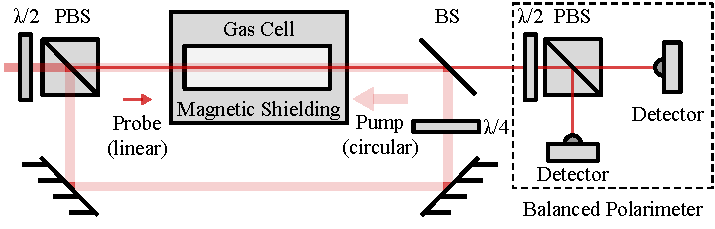
\includegraphics[width=\linewidth]{part1/Figs/PolSpecSchematic.pdf}
\caption{A schematic of \gls{ps} with a balanced polarimeter.
The power balance between the probe and the pump beam is controlled with the left-most $\lambda/2$ phase retarder and \gls{pbs}.
The $\lambda/4$ retarder is adjusted to produce a circularly polarised pump beam.
The non-polarising beamsplitter (BS) is used to counter-propagate the pump beam through the atomic sample without altering the polarisation of the circular pump or linear probe.
The final $\lambda/2$ retarder, \gls{pbs} and the detectors form the balanced polarimeter that monitors the polarisation rotation of the probe.}
\label{figure:pol_spec_schematic}
\end{figure}

The circularly polarised pump beam induces circular birefringence in the atomic sample by partial optical pumping of the sample into one of the extreme hyperfine sublevels, $m_F=\pm F$, where $m_F$ labels the hyperfine sublevel and $F$ is the atomic angular momentum number.
This partial optical pumping, referred to here as the anisotropy of the medium, results in unequal absorption coefficients for each circular polarisation.
The linearly polarised probe beam can be decomposed into two equal and oppositely circularly polarised components which undergo different absorption due to the anisotropy, such that when recombined after passing through the atomic sample the probe beam becomes elliptically polarised with an angle different to that of the original linear polarisation.

Consider the electric field of the probe beam before it enters the atomic sample at an angle $\phi$ to the $x$ axis:
\begin{equation}
\vec{E}=E_0\big(\cos{\phi}\,\hat{x}+\sin{\phi}\,\hat{y}\big)
\end{equation}
which can be expressed in terms of the circularly polarised basis vectors, $(\hat{x}\pm i\hat{y})$,
\begin{equation}
\vec{E} = \frac{E_0}{2}e^{-i\phi}(\hat{x}+i\hat{y}) + \frac{E_0}{2}e^{+i\phi}(\hat{x}-i\hat{y})
\end{equation}

After propagating through an atomic sample of length $L$ with refractive indices for the circular polarisation components of $n_\pm$, and absorption coefficients of $\alpha_\pm$ the electric field becomes
\begin{align}
\vec{E}\  = \ &\frac{E_0}{2}e^{-i\phi}\,\exp\left[\frac{i\omega n_+ L}{c} - \frac{\alpha_+ L}{2}\right](\hat{x}+i\hat{y})\quad +\quad \frac{E_0}{2}e^{+i\phi}\,\exp\left[\frac{i\omega n_- L}{c} - \frac{\alpha_- L}{2}\right](\hat{x}-i\hat{y}) \notag\\ 
\  = \ &\frac{E_0}{2} e^{-i\phi}\,\exp\left[\frac{i\omega L}{2c}(n_+-n_-) + \frac{i\omega L}{2c}(n_+ + n_-) - \frac{L}{4}(\alpha_+ -\alpha_-) - \frac{L}{4}(\alpha_+ + \alpha_-)\right](\hat{x}+i\hat{y})\ +\notag\\
&\frac{E_0}{2} e^{+i\phi}\,\exp\left[-\frac{i\omega L}{2c}(n_+-n_-) + \frac{i\omega L}{2c}(n_-+n_+) + \frac{L}{4}(\alpha_+-\alpha_-) - \frac{L}{4}(\alpha_-+\alpha_+) \right](\hat{x}-i\hat{y}) \notag\\
\  = \ &\frac{E_0}{2} \exp\left[\frac{i\omega L}{2c}(n_+ + n_-) - \frac{L}{4}(\alpha_+ + \alpha_-)\right] \left\{ e^{-i(\phi - \Omega)}\, \, (\hat{x}+i\hat{y})\ + e^{+i(\phi-\Omega)}\,(\hat{x}-i\hat{y})\right\},\label{equation:elliptically_polarised}
\end{align}
where
\begin{equation}
\Omega = \frac{\omega L}{2c}(n_+-n_-) + i\frac{L}{4}(\alpha_+ -\alpha_-).
\end{equation}
Equation \ref{equation:elliptically_polarised} represents elliptically polarised light with the major axis at an angle of $\theta = \phi + \Omega$ to the $x$-axis.

The horizontal and vertical polarisation components of the beam are separated by the \gls{pbs},
\begin{align}
\vec{E} = &\frac{E_0}{2} \exp\left[\frac{i\omega L}{2c}(N_+ + n_-) - \frac{L}{4}(\alpha_++\alpha_-)\right]\ \left[ \hat{x} \left(e^{-i(\phi-\Omega)}+e^{-i(\phi-\Omega)}\right) + i\hat{y} \left(e^{-i(\phi-\Omega)}-e^{-i(\phi-\Omega)}\right)\right]\notag\\
 = & E_0 \exp\left[\frac{i\omega L}{2c}(N_+ + n_-) - \frac{L}{4}(\alpha_++\alpha_-)\right] \bigg[ \hat{x} \cos(\phi-\Omega) + \hat{y} \sin(\phi-\Omega)\bigg],
\end{align}
and the intensity of the beams are then detected by photodetectors,
\begin{align}
I_x &= |E_x|^2 \notag \\
& = \left|E_0 \exp\left[\frac{i\omega L}{2c}(N_+ + n_-) - \frac{L}{4}(\alpha_++\alpha_-)\right] \cos(\phi-\Omega) \right|^2 \notag \\
& = E_0^2\left| \exp\left[\frac{i\omega L}{2c}(N_+ + n_-)\right]\exp\left[-\frac{L}{4}(\alpha_++\alpha_-)\right] \right|^2 \cos\bigg(\phi-\Omega\bigg) \cos\bigg(\overline{\phi-\Omega}\bigg) \notag \\
& = E_0^2 \exp\left[-\frac{L}{2}(\alpha_++\alpha_-)\right] \cos\bigg(\phi-\frac{\omega L}{2c}(n_+-n_-) + i\frac{L}{4}(\alpha_+ -\alpha_-)\bigg) \cos\bigg(\phi-\frac{\omega L}{2c}(n_+-n_-) - i\frac{L}{4}(\alpha_+ -\alpha_-)\bigg) \notag \\
& = \frac{E_0^2}{2} \exp\left[-\frac{L}{2}(\alpha_++\alpha_-)\right] \left[\cos\bigg(2i\frac{L}{4}(\alpha_+ -\alpha_-)\bigg) + \cos\bigg(2\phi-2\frac{\omega L}{2c}(n_+-n_-)\bigg)\right] \\
\notag\\
I_y &= |E_y|^2 \notag \\
& = \left|E_0 \exp\left[\frac{i\omega L}{2c}(N_+ + n_-) - \frac{L}{4}(\alpha_++\alpha_-)\right] \sin(\phi-\Omega) \right|^2 \notag \\
& = \frac{E_0^2}{2} \exp\left[-\frac{L}{2}(\alpha_++\alpha_-)\right] \left[\cos\bigg(2i\frac{L}{4}(\alpha_+ -\alpha_-)\bigg) - \cos\bigg(2\phi-2\frac{\omega L}{2c}(n_+-n_-)\bigg)\right]
\end{align}
and subtracted by electronics to generate the error signal,
\begin{align}
\epsilon =\ &I_y - I_x = E_y^2 - E_x^2 \notag \\
=\ &E_0^2 \exp\left[-\frac{L}{2}(\alpha_++\alpha_-)\right] \cos\bigg(2\phi-2\frac{\omega L}{2c}(n_+-n_-)\bigg).
\end{align}

The spectral profile of $(\alpha_+-\alpha_-)$ is a power-broadened Lorentzian~\cite{pearman_polarization_2002},
\begin{equation}
\alpha_+ - \alpha_- = \frac{\Delta\alpha_0}{1+x^2},
\end{equation}
where $x=\frac{\omega_0-\omega}{\Gamma/2}$ is the detuning scaled by the atomic linewidth $\Gamma$, and $\Delta\alpha_0$ is the maximum difference in absorption coefficients at the atomic resonance.
The absorption cooefficients and refractive indices are related via the Kramers-Kronig dispersion relation~\cite{demtroder_laser_2014},
\begin{equation}
n_+ - n_- = \frac{c}{\omega_0} \Delta\alpha_0 \frac{x}{1+x^2}.
\end{equation}
Typically the polarisation rotation induced by the medium is small and is maximised when $\phi=\frac{\pi}{4}$ giving the approximate error signal,
\begin{equation}
\epsilon \simeq - I_0 e^{-L(\alpha_++\alpha_-)/2}\left( L \Delta\alpha_0 \frac{x}{1+x^2}\right)
\end{equation}

\Gls{ps} produces a dispersion shaped spectrum about the atomic resonance with zero background, as shown in Figure~\ref{figure:polspecspectrum}, and is ideal for laser locking due to the large capture range and steep gradient near the resonance.
Unlike \gls{pdh}, \gls{ps} acts as an absolute reference as it tied to the frequency of the atomic-ensemble reference rather than a cavity.

\begin{figure}
\center
%% Creator: Matplotlib, PGF backend
%%
%% To include the figure in your LaTeX document, write
%%   \input{<filename>.pgf}
%%
%% Make sure the required packages are loaded in your preamble
%%   \usepackage{pgf}
%%
%% Figures using additional raster images can only be included by \input if
%% they are in the same directory as the main LaTeX file. For loading figures
%% from other directories you can use the `import` package
%%   \usepackage{import}
%% and then include the figures with
%%   \import{<path to file>}{<filename>.pgf}
%%
%% Matplotlib used the following preamble
%%
\begingroup%
\makeatletter%
\begin{pgfpicture}%
\pgfpathrectangle{\pgfpointorigin}{\pgfqpoint{5.710000in}{3.524691in}}%
\pgfusepath{use as bounding box, clip}%
\begin{pgfscope}%
\pgfsetbuttcap%
\pgfsetmiterjoin%
\definecolor{currentfill}{rgb}{1.000000,1.000000,1.000000}%
\pgfsetfillcolor{currentfill}%
\pgfsetlinewidth{0.000000pt}%
\definecolor{currentstroke}{rgb}{1.000000,1.000000,1.000000}%
\pgfsetstrokecolor{currentstroke}%
\pgfsetdash{}{0pt}%
\pgfpathmoveto{\pgfqpoint{0.000000in}{0.000000in}}%
\pgfpathlineto{\pgfqpoint{5.710000in}{0.000000in}}%
\pgfpathlineto{\pgfqpoint{5.710000in}{3.524691in}}%
\pgfpathlineto{\pgfqpoint{0.000000in}{3.524691in}}%
\pgfpathclose%
\pgfusepath{fill}%
\end{pgfscope}%
\begin{pgfscope}%
\pgfsetbuttcap%
\pgfsetmiterjoin%
\definecolor{currentfill}{rgb}{1.000000,1.000000,1.000000}%
\pgfsetfillcolor{currentfill}%
\pgfsetlinewidth{0.000000pt}%
\definecolor{currentstroke}{rgb}{0.000000,0.000000,0.000000}%
\pgfsetstrokecolor{currentstroke}%
\pgfsetstrokeopacity{0.000000}%
\pgfsetdash{}{0pt}%
\pgfpathmoveto{\pgfqpoint{0.467749in}{0.521851in}}%
\pgfpathlineto{\pgfqpoint{5.560000in}{0.521851in}}%
\pgfpathlineto{\pgfqpoint{5.560000in}{3.374691in}}%
\pgfpathlineto{\pgfqpoint{0.467749in}{3.374691in}}%
\pgfpathclose%
\pgfusepath{fill}%
\end{pgfscope}%
\begin{pgfscope}%
\pgfpathrectangle{\pgfqpoint{0.467749in}{0.521851in}}{\pgfqpoint{5.092251in}{2.852840in}} %
\pgfusepath{clip}%
\pgfsetrectcap%
\pgfsetroundjoin%
\pgfsetlinewidth{1.003750pt}%
\definecolor{currentstroke}{rgb}{0.309804,0.478431,0.682353}%
\pgfsetstrokecolor{currentstroke}%
\pgfsetdash{}{0pt}%
\pgfpathmoveto{\pgfqpoint{0.467047in}{1.399753in}}%
\pgfpathlineto{\pgfqpoint{0.470095in}{1.400941in}}%
\pgfpathlineto{\pgfqpoint{0.473143in}{1.399372in}}%
\pgfpathlineto{\pgfqpoint{0.474158in}{1.400561in}}%
\pgfpathlineto{\pgfqpoint{0.475174in}{1.399515in}}%
\pgfpathlineto{\pgfqpoint{0.476190in}{1.400941in}}%
\pgfpathlineto{\pgfqpoint{0.477206in}{1.399562in}}%
\pgfpathlineto{\pgfqpoint{0.478222in}{1.401083in}}%
\pgfpathlineto{\pgfqpoint{0.479238in}{1.398327in}}%
\pgfpathlineto{\pgfqpoint{0.481270in}{1.400941in}}%
\pgfpathlineto{\pgfqpoint{0.482286in}{1.399087in}}%
\pgfpathlineto{\pgfqpoint{0.485333in}{1.403032in}}%
\pgfpathlineto{\pgfqpoint{0.487365in}{1.400038in}}%
\pgfpathlineto{\pgfqpoint{0.488381in}{1.401273in}}%
\pgfpathlineto{\pgfqpoint{0.489397in}{1.400465in}}%
\pgfpathlineto{\pgfqpoint{0.490413in}{1.401606in}}%
\pgfpathlineto{\pgfqpoint{0.491429in}{1.399705in}}%
\pgfpathlineto{\pgfqpoint{0.492444in}{1.401939in}}%
\pgfpathlineto{\pgfqpoint{0.494476in}{1.399705in}}%
\pgfpathlineto{\pgfqpoint{0.496508in}{1.400703in}}%
\pgfpathlineto{\pgfqpoint{0.503619in}{1.401273in}}%
\pgfpathlineto{\pgfqpoint{0.504635in}{1.400133in}}%
\pgfpathlineto{\pgfqpoint{0.507683in}{1.401178in}}%
\pgfpathlineto{\pgfqpoint{0.510730in}{1.399467in}}%
\pgfpathlineto{\pgfqpoint{0.512762in}{1.401464in}}%
\pgfpathlineto{\pgfqpoint{0.513778in}{1.400323in}}%
\pgfpathlineto{\pgfqpoint{0.515810in}{1.400941in}}%
\pgfpathlineto{\pgfqpoint{0.516826in}{1.400180in}}%
\pgfpathlineto{\pgfqpoint{0.517842in}{1.402177in}}%
\pgfpathlineto{\pgfqpoint{0.518857in}{1.400323in}}%
\pgfpathlineto{\pgfqpoint{0.521905in}{1.401464in}}%
\pgfpathlineto{\pgfqpoint{0.523937in}{1.400608in}}%
\pgfpathlineto{\pgfqpoint{0.525969in}{1.400608in}}%
\pgfpathlineto{\pgfqpoint{0.528000in}{1.402177in}}%
\pgfpathlineto{\pgfqpoint{0.530032in}{1.401131in}}%
\pgfpathlineto{\pgfqpoint{0.531048in}{1.402414in}}%
\pgfpathlineto{\pgfqpoint{0.532064in}{1.399277in}}%
\pgfpathlineto{\pgfqpoint{0.534096in}{1.401226in}}%
\pgfpathlineto{\pgfqpoint{0.538159in}{1.399230in}}%
\pgfpathlineto{\pgfqpoint{0.541207in}{1.401083in}}%
\pgfpathlineto{\pgfqpoint{0.542223in}{1.403032in}}%
\pgfpathlineto{\pgfqpoint{0.544255in}{1.400085in}}%
\pgfpathlineto{\pgfqpoint{0.547302in}{1.401939in}}%
\pgfpathlineto{\pgfqpoint{0.552382in}{1.400561in}}%
\pgfpathlineto{\pgfqpoint{0.557461in}{1.400656in}}%
\pgfpathlineto{\pgfqpoint{0.558477in}{1.401891in}}%
\pgfpathlineto{\pgfqpoint{0.559493in}{1.400133in}}%
\pgfpathlineto{\pgfqpoint{0.562541in}{1.400608in}}%
\pgfpathlineto{\pgfqpoint{0.563556in}{1.399515in}}%
\pgfpathlineto{\pgfqpoint{0.566604in}{1.401749in}}%
\pgfpathlineto{\pgfqpoint{0.567620in}{1.400418in}}%
\pgfpathlineto{\pgfqpoint{0.568636in}{1.402414in}}%
\pgfpathlineto{\pgfqpoint{0.570668in}{1.401464in}}%
\pgfpathlineto{\pgfqpoint{0.572699in}{1.402462in}}%
\pgfpathlineto{\pgfqpoint{0.573715in}{1.402842in}}%
\pgfpathlineto{\pgfqpoint{0.574731in}{1.399753in}}%
\pgfpathlineto{\pgfqpoint{0.575747in}{1.400893in}}%
\pgfpathlineto{\pgfqpoint{0.576763in}{1.400275in}}%
\pgfpathlineto{\pgfqpoint{0.578795in}{1.402462in}}%
\pgfpathlineto{\pgfqpoint{0.580827in}{1.400275in}}%
\pgfpathlineto{\pgfqpoint{0.582858in}{1.400180in}}%
\pgfpathlineto{\pgfqpoint{0.583874in}{1.402414in}}%
\pgfpathlineto{\pgfqpoint{0.585906in}{1.400133in}}%
\pgfpathlineto{\pgfqpoint{0.588954in}{1.401986in}}%
\pgfpathlineto{\pgfqpoint{0.589970in}{1.399658in}}%
\pgfpathlineto{\pgfqpoint{0.590985in}{1.401654in}}%
\pgfpathlineto{\pgfqpoint{0.593017in}{1.399610in}}%
\pgfpathlineto{\pgfqpoint{0.595049in}{1.401273in}}%
\pgfpathlineto{\pgfqpoint{0.596065in}{1.402129in}}%
\pgfpathlineto{\pgfqpoint{0.597081in}{1.399895in}}%
\pgfpathlineto{\pgfqpoint{0.598097in}{1.400513in}}%
\pgfpathlineto{\pgfqpoint{0.599113in}{1.403127in}}%
\pgfpathlineto{\pgfqpoint{0.600128in}{1.400180in}}%
\pgfpathlineto{\pgfqpoint{0.601144in}{1.401796in}}%
\pgfpathlineto{\pgfqpoint{0.602160in}{1.399895in}}%
\pgfpathlineto{\pgfqpoint{0.605208in}{1.401559in}}%
\pgfpathlineto{\pgfqpoint{0.608255in}{1.400656in}}%
\pgfpathlineto{\pgfqpoint{0.609271in}{1.402794in}}%
\pgfpathlineto{\pgfqpoint{0.610287in}{1.402319in}}%
\pgfpathlineto{\pgfqpoint{0.611303in}{1.400180in}}%
\pgfpathlineto{\pgfqpoint{0.612319in}{1.402319in}}%
\pgfpathlineto{\pgfqpoint{0.616383in}{1.400561in}}%
\pgfpathlineto{\pgfqpoint{0.618414in}{1.400941in}}%
\pgfpathlineto{\pgfqpoint{0.619430in}{1.402462in}}%
\pgfpathlineto{\pgfqpoint{0.620446in}{1.400941in}}%
\pgfpathlineto{\pgfqpoint{0.622478in}{1.401083in}}%
\pgfpathlineto{\pgfqpoint{0.623494in}{1.400846in}}%
\pgfpathlineto{\pgfqpoint{0.624510in}{1.402224in}}%
\pgfpathlineto{\pgfqpoint{0.625526in}{1.400608in}}%
\pgfpathlineto{\pgfqpoint{0.629589in}{1.401796in}}%
\pgfpathlineto{\pgfqpoint{0.633653in}{1.400893in}}%
\pgfpathlineto{\pgfqpoint{0.635684in}{1.402034in}}%
\pgfpathlineto{\pgfqpoint{0.641780in}{1.401511in}}%
\pgfpathlineto{\pgfqpoint{0.644827in}{1.400038in}}%
\pgfpathlineto{\pgfqpoint{0.648891in}{1.402509in}}%
\pgfpathlineto{\pgfqpoint{0.650923in}{1.401891in}}%
\pgfpathlineto{\pgfqpoint{0.651939in}{1.403317in}}%
\pgfpathlineto{\pgfqpoint{0.652954in}{1.401321in}}%
\pgfpathlineto{\pgfqpoint{0.653970in}{1.402129in}}%
\pgfpathlineto{\pgfqpoint{0.654986in}{1.400846in}}%
\pgfpathlineto{\pgfqpoint{0.656002in}{1.403032in}}%
\pgfpathlineto{\pgfqpoint{0.657018in}{1.400941in}}%
\pgfpathlineto{\pgfqpoint{0.658034in}{1.402699in}}%
\pgfpathlineto{\pgfqpoint{0.659050in}{1.400038in}}%
\pgfpathlineto{\pgfqpoint{0.660066in}{1.402509in}}%
\pgfpathlineto{\pgfqpoint{0.663113in}{1.401273in}}%
\pgfpathlineto{\pgfqpoint{0.664129in}{1.402129in}}%
\pgfpathlineto{\pgfqpoint{0.665145in}{1.400656in}}%
\pgfpathlineto{\pgfqpoint{0.668193in}{1.402177in}}%
\pgfpathlineto{\pgfqpoint{0.670225in}{1.402224in}}%
\pgfpathlineto{\pgfqpoint{0.672256in}{1.401891in}}%
\pgfpathlineto{\pgfqpoint{0.673272in}{1.400513in}}%
\pgfpathlineto{\pgfqpoint{0.674288in}{1.402842in}}%
\pgfpathlineto{\pgfqpoint{0.675304in}{1.400465in}}%
\pgfpathlineto{\pgfqpoint{0.677336in}{1.401368in}}%
\pgfpathlineto{\pgfqpoint{0.681399in}{1.402604in}}%
\pgfpathlineto{\pgfqpoint{0.682415in}{1.403270in}}%
\pgfpathlineto{\pgfqpoint{0.684447in}{1.402034in}}%
\pgfpathlineto{\pgfqpoint{0.688511in}{1.401321in}}%
\pgfpathlineto{\pgfqpoint{0.692574in}{1.401986in}}%
\pgfpathlineto{\pgfqpoint{0.694606in}{1.401559in}}%
\pgfpathlineto{\pgfqpoint{0.697653in}{1.403270in}}%
\pgfpathlineto{\pgfqpoint{0.699685in}{1.400418in}}%
\pgfpathlineto{\pgfqpoint{0.702733in}{1.402699in}}%
\pgfpathlineto{\pgfqpoint{0.706796in}{1.400846in}}%
\pgfpathlineto{\pgfqpoint{0.707812in}{1.403317in}}%
\pgfpathlineto{\pgfqpoint{0.710860in}{1.401511in}}%
\pgfpathlineto{\pgfqpoint{0.711876in}{1.403222in}}%
\pgfpathlineto{\pgfqpoint{0.715939in}{1.401178in}}%
\pgfpathlineto{\pgfqpoint{0.717971in}{1.402224in}}%
\pgfpathlineto{\pgfqpoint{0.720003in}{1.402224in}}%
\pgfpathlineto{\pgfqpoint{0.721019in}{1.399800in}}%
\pgfpathlineto{\pgfqpoint{0.723051in}{1.401844in}}%
\pgfpathlineto{\pgfqpoint{0.724067in}{1.400798in}}%
\pgfpathlineto{\pgfqpoint{0.725082in}{1.402842in}}%
\pgfpathlineto{\pgfqpoint{0.727114in}{1.401701in}}%
\pgfpathlineto{\pgfqpoint{0.728130in}{1.403365in}}%
\pgfpathlineto{\pgfqpoint{0.729146in}{1.402034in}}%
\pgfpathlineto{\pgfqpoint{0.730162in}{1.404173in}}%
\pgfpathlineto{\pgfqpoint{0.731178in}{1.400275in}}%
\pgfpathlineto{\pgfqpoint{0.733210in}{1.401559in}}%
\pgfpathlineto{\pgfqpoint{0.737273in}{1.403602in}}%
\pgfpathlineto{\pgfqpoint{0.739305in}{1.401416in}}%
\pgfpathlineto{\pgfqpoint{0.740321in}{1.400941in}}%
\pgfpathlineto{\pgfqpoint{0.742352in}{1.402462in}}%
\pgfpathlineto{\pgfqpoint{0.743368in}{1.401986in}}%
\pgfpathlineto{\pgfqpoint{0.744384in}{1.402937in}}%
\pgfpathlineto{\pgfqpoint{0.746416in}{1.400941in}}%
\pgfpathlineto{\pgfqpoint{0.748448in}{1.402177in}}%
\pgfpathlineto{\pgfqpoint{0.752511in}{1.403792in}}%
\pgfpathlineto{\pgfqpoint{0.753527in}{1.402319in}}%
\pgfpathlineto{\pgfqpoint{0.754543in}{1.403650in}}%
\pgfpathlineto{\pgfqpoint{0.755559in}{1.401416in}}%
\pgfpathlineto{\pgfqpoint{0.756575in}{1.403032in}}%
\pgfpathlineto{\pgfqpoint{0.758607in}{1.400846in}}%
\pgfpathlineto{\pgfqpoint{0.760638in}{1.402794in}}%
\pgfpathlineto{\pgfqpoint{0.762670in}{1.403317in}}%
\pgfpathlineto{\pgfqpoint{0.765718in}{1.400228in}}%
\pgfpathlineto{\pgfqpoint{0.767750in}{1.401796in}}%
\pgfpathlineto{\pgfqpoint{0.769781in}{1.402177in}}%
\pgfpathlineto{\pgfqpoint{0.771813in}{1.403935in}}%
\pgfpathlineto{\pgfqpoint{0.774861in}{1.399990in}}%
\pgfpathlineto{\pgfqpoint{0.775877in}{1.404363in}}%
\pgfpathlineto{\pgfqpoint{0.777909in}{1.401891in}}%
\pgfpathlineto{\pgfqpoint{0.778924in}{1.401321in}}%
\pgfpathlineto{\pgfqpoint{0.779940in}{1.403270in}}%
\pgfpathlineto{\pgfqpoint{0.781972in}{1.401796in}}%
\pgfpathlineto{\pgfqpoint{0.784004in}{1.402224in}}%
\pgfpathlineto{\pgfqpoint{0.789083in}{1.402129in}}%
\pgfpathlineto{\pgfqpoint{0.790099in}{1.403697in}}%
\pgfpathlineto{\pgfqpoint{0.792131in}{1.401559in}}%
\pgfpathlineto{\pgfqpoint{0.793147in}{1.402177in}}%
\pgfpathlineto{\pgfqpoint{0.794163in}{1.404173in}}%
\pgfpathlineto{\pgfqpoint{0.795179in}{1.400703in}}%
\pgfpathlineto{\pgfqpoint{0.797210in}{1.402509in}}%
\pgfpathlineto{\pgfqpoint{0.799242in}{1.401368in}}%
\pgfpathlineto{\pgfqpoint{0.801274in}{1.402984in}}%
\pgfpathlineto{\pgfqpoint{0.802290in}{1.400846in}}%
\pgfpathlineto{\pgfqpoint{0.803306in}{1.404125in}}%
\pgfpathlineto{\pgfqpoint{0.804322in}{1.401416in}}%
\pgfpathlineto{\pgfqpoint{0.807369in}{1.402889in}}%
\pgfpathlineto{\pgfqpoint{0.810417in}{1.402747in}}%
\pgfpathlineto{\pgfqpoint{0.811433in}{1.400703in}}%
\pgfpathlineto{\pgfqpoint{0.812449in}{1.403032in}}%
\pgfpathlineto{\pgfqpoint{0.813465in}{1.401321in}}%
\pgfpathlineto{\pgfqpoint{0.815496in}{1.404553in}}%
\pgfpathlineto{\pgfqpoint{0.817528in}{1.402034in}}%
\pgfpathlineto{\pgfqpoint{0.818544in}{1.402937in}}%
\pgfpathlineto{\pgfqpoint{0.819560in}{1.400941in}}%
\pgfpathlineto{\pgfqpoint{0.821592in}{1.403080in}}%
\pgfpathlineto{\pgfqpoint{0.824639in}{1.402177in}}%
\pgfpathlineto{\pgfqpoint{0.827687in}{1.401321in}}%
\pgfpathlineto{\pgfqpoint{0.829719in}{1.402842in}}%
\pgfpathlineto{\pgfqpoint{0.830735in}{1.403032in}}%
\pgfpathlineto{\pgfqpoint{0.832766in}{1.401273in}}%
\pgfpathlineto{\pgfqpoint{0.833782in}{1.402984in}}%
\pgfpathlineto{\pgfqpoint{0.834798in}{1.400751in}}%
\pgfpathlineto{\pgfqpoint{0.835814in}{1.404553in}}%
\pgfpathlineto{\pgfqpoint{0.836830in}{1.402842in}}%
\pgfpathlineto{\pgfqpoint{0.837846in}{1.404220in}}%
\pgfpathlineto{\pgfqpoint{0.838862in}{1.401368in}}%
\pgfpathlineto{\pgfqpoint{0.840893in}{1.403127in}}%
\pgfpathlineto{\pgfqpoint{0.841909in}{1.402081in}}%
\pgfpathlineto{\pgfqpoint{0.842925in}{1.403792in}}%
\pgfpathlineto{\pgfqpoint{0.844957in}{1.402794in}}%
\pgfpathlineto{\pgfqpoint{0.850036in}{1.402984in}}%
\pgfpathlineto{\pgfqpoint{0.851052in}{1.403460in}}%
\pgfpathlineto{\pgfqpoint{0.854100in}{1.401178in}}%
\pgfpathlineto{\pgfqpoint{0.855116in}{1.402462in}}%
\pgfpathlineto{\pgfqpoint{0.856132in}{1.401891in}}%
\pgfpathlineto{\pgfqpoint{0.857148in}{1.403175in}}%
\pgfpathlineto{\pgfqpoint{0.858164in}{1.402319in}}%
\pgfpathlineto{\pgfqpoint{0.859179in}{1.403602in}}%
\pgfpathlineto{\pgfqpoint{0.860195in}{1.401511in}}%
\pgfpathlineto{\pgfqpoint{0.862227in}{1.402794in}}%
\pgfpathlineto{\pgfqpoint{0.864259in}{1.401226in}}%
\pgfpathlineto{\pgfqpoint{0.866291in}{1.403792in}}%
\pgfpathlineto{\pgfqpoint{0.868322in}{1.402367in}}%
\pgfpathlineto{\pgfqpoint{0.870354in}{1.404363in}}%
\pgfpathlineto{\pgfqpoint{0.873402in}{1.401083in}}%
\pgfpathlineto{\pgfqpoint{0.875434in}{1.403127in}}%
\pgfpathlineto{\pgfqpoint{0.877465in}{1.401606in}}%
\pgfpathlineto{\pgfqpoint{0.878481in}{1.401701in}}%
\pgfpathlineto{\pgfqpoint{0.879497in}{1.403840in}}%
\pgfpathlineto{\pgfqpoint{0.880513in}{1.402129in}}%
\pgfpathlineto{\pgfqpoint{0.882545in}{1.402937in}}%
\pgfpathlineto{\pgfqpoint{0.891688in}{1.401749in}}%
\pgfpathlineto{\pgfqpoint{0.892704in}{1.403175in}}%
\pgfpathlineto{\pgfqpoint{0.894735in}{1.400561in}}%
\pgfpathlineto{\pgfqpoint{0.896767in}{1.403888in}}%
\pgfpathlineto{\pgfqpoint{0.898799in}{1.403365in}}%
\pgfpathlineto{\pgfqpoint{0.899815in}{1.404268in}}%
\pgfpathlineto{\pgfqpoint{0.902863in}{1.401606in}}%
\pgfpathlineto{\pgfqpoint{0.903878in}{1.404220in}}%
\pgfpathlineto{\pgfqpoint{0.905910in}{1.403460in}}%
\pgfpathlineto{\pgfqpoint{0.906926in}{1.404410in}}%
\pgfpathlineto{\pgfqpoint{0.909974in}{1.402129in}}%
\pgfpathlineto{\pgfqpoint{0.910990in}{1.402984in}}%
\pgfpathlineto{\pgfqpoint{0.912006in}{1.402177in}}%
\pgfpathlineto{\pgfqpoint{0.916069in}{1.405171in}}%
\pgfpathlineto{\pgfqpoint{0.923180in}{1.402509in}}%
\pgfpathlineto{\pgfqpoint{0.925212in}{1.404696in}}%
\pgfpathlineto{\pgfqpoint{0.926228in}{1.402557in}}%
\pgfpathlineto{\pgfqpoint{0.927244in}{1.403365in}}%
\pgfpathlineto{\pgfqpoint{0.928260in}{1.402034in}}%
\pgfpathlineto{\pgfqpoint{0.930291in}{1.404363in}}%
\pgfpathlineto{\pgfqpoint{0.933339in}{1.403555in}}%
\pgfpathlineto{\pgfqpoint{0.936387in}{1.404078in}}%
\pgfpathlineto{\pgfqpoint{0.938419in}{1.402794in}}%
\pgfpathlineto{\pgfqpoint{0.939434in}{1.403270in}}%
\pgfpathlineto{\pgfqpoint{0.940450in}{1.402462in}}%
\pgfpathlineto{\pgfqpoint{0.941466in}{1.404553in}}%
\pgfpathlineto{\pgfqpoint{0.943498in}{1.402509in}}%
\pgfpathlineto{\pgfqpoint{0.944514in}{1.402177in}}%
\pgfpathlineto{\pgfqpoint{0.946546in}{1.404030in}}%
\pgfpathlineto{\pgfqpoint{0.948577in}{1.404173in}}%
\pgfpathlineto{\pgfqpoint{0.949593in}{1.402509in}}%
\pgfpathlineto{\pgfqpoint{0.950609in}{1.404315in}}%
\pgfpathlineto{\pgfqpoint{0.952641in}{1.402604in}}%
\pgfpathlineto{\pgfqpoint{0.953657in}{1.403270in}}%
\pgfpathlineto{\pgfqpoint{0.954673in}{1.402367in}}%
\pgfpathlineto{\pgfqpoint{0.956705in}{1.404458in}}%
\pgfpathlineto{\pgfqpoint{0.957720in}{1.402319in}}%
\pgfpathlineto{\pgfqpoint{0.959752in}{1.404410in}}%
\pgfpathlineto{\pgfqpoint{0.962800in}{1.401939in}}%
\pgfpathlineto{\pgfqpoint{0.964832in}{1.405503in}}%
\pgfpathlineto{\pgfqpoint{0.967879in}{1.403412in}}%
\pgfpathlineto{\pgfqpoint{0.970927in}{1.404315in}}%
\pgfpathlineto{\pgfqpoint{0.971943in}{1.403460in}}%
\pgfpathlineto{\pgfqpoint{0.972959in}{1.404410in}}%
\pgfpathlineto{\pgfqpoint{0.974990in}{1.401606in}}%
\pgfpathlineto{\pgfqpoint{0.976006in}{1.403745in}}%
\pgfpathlineto{\pgfqpoint{0.978038in}{1.402937in}}%
\pgfpathlineto{\pgfqpoint{0.980070in}{1.404505in}}%
\pgfpathlineto{\pgfqpoint{0.983118in}{1.403602in}}%
\pgfpathlineto{\pgfqpoint{0.984133in}{1.404030in}}%
\pgfpathlineto{\pgfqpoint{0.986165in}{1.403650in}}%
\pgfpathlineto{\pgfqpoint{0.987181in}{1.404886in}}%
\pgfpathlineto{\pgfqpoint{0.988197in}{1.402794in}}%
\pgfpathlineto{\pgfqpoint{0.989213in}{1.403983in}}%
\pgfpathlineto{\pgfqpoint{0.991245in}{1.402747in}}%
\pgfpathlineto{\pgfqpoint{0.994292in}{1.404173in}}%
\pgfpathlineto{\pgfqpoint{1.000388in}{1.403080in}}%
\pgfpathlineto{\pgfqpoint{1.001404in}{1.405266in}}%
\pgfpathlineto{\pgfqpoint{1.002419in}{1.404553in}}%
\pgfpathlineto{\pgfqpoint{1.003435in}{1.405361in}}%
\pgfpathlineto{\pgfqpoint{1.004451in}{1.402034in}}%
\pgfpathlineto{\pgfqpoint{1.007499in}{1.402937in}}%
\pgfpathlineto{\pgfqpoint{1.008515in}{1.402889in}}%
\pgfpathlineto{\pgfqpoint{1.010547in}{1.401606in}}%
\pgfpathlineto{\pgfqpoint{1.012578in}{1.404268in}}%
\pgfpathlineto{\pgfqpoint{1.013594in}{1.402937in}}%
\pgfpathlineto{\pgfqpoint{1.014610in}{1.403935in}}%
\pgfpathlineto{\pgfqpoint{1.015626in}{1.402557in}}%
\pgfpathlineto{\pgfqpoint{1.018674in}{1.403935in}}%
\pgfpathlineto{\pgfqpoint{1.021721in}{1.402937in}}%
\pgfpathlineto{\pgfqpoint{1.023753in}{1.403317in}}%
\pgfpathlineto{\pgfqpoint{1.024769in}{1.402177in}}%
\pgfpathlineto{\pgfqpoint{1.025785in}{1.403507in}}%
\pgfpathlineto{\pgfqpoint{1.026801in}{1.402604in}}%
\pgfpathlineto{\pgfqpoint{1.028832in}{1.403460in}}%
\pgfpathlineto{\pgfqpoint{1.029848in}{1.403460in}}%
\pgfpathlineto{\pgfqpoint{1.031880in}{1.405076in}}%
\pgfpathlineto{\pgfqpoint{1.033912in}{1.403460in}}%
\pgfpathlineto{\pgfqpoint{1.035944in}{1.404505in}}%
\pgfpathlineto{\pgfqpoint{1.036960in}{1.403317in}}%
\pgfpathlineto{\pgfqpoint{1.037975in}{1.404173in}}%
\pgfpathlineto{\pgfqpoint{1.040007in}{1.402889in}}%
\pgfpathlineto{\pgfqpoint{1.043055in}{1.402557in}}%
\pgfpathlineto{\pgfqpoint{1.045087in}{1.403650in}}%
\pgfpathlineto{\pgfqpoint{1.046103in}{1.403412in}}%
\pgfpathlineto{\pgfqpoint{1.048134in}{1.404505in}}%
\pgfpathlineto{\pgfqpoint{1.049150in}{1.402699in}}%
\pgfpathlineto{\pgfqpoint{1.052198in}{1.404315in}}%
\pgfpathlineto{\pgfqpoint{1.054230in}{1.402747in}}%
\pgfpathlineto{\pgfqpoint{1.056261in}{1.404363in}}%
\pgfpathlineto{\pgfqpoint{1.059309in}{1.402889in}}%
\pgfpathlineto{\pgfqpoint{1.062357in}{1.404696in}}%
\pgfpathlineto{\pgfqpoint{1.064388in}{1.403697in}}%
\pgfpathlineto{\pgfqpoint{1.065404in}{1.405313in}}%
\pgfpathlineto{\pgfqpoint{1.066420in}{1.402984in}}%
\pgfpathlineto{\pgfqpoint{1.068452in}{1.404078in}}%
\pgfpathlineto{\pgfqpoint{1.070484in}{1.402604in}}%
\pgfpathlineto{\pgfqpoint{1.071500in}{1.404743in}}%
\pgfpathlineto{\pgfqpoint{1.073531in}{1.402319in}}%
\pgfpathlineto{\pgfqpoint{1.074547in}{1.404981in}}%
\pgfpathlineto{\pgfqpoint{1.076579in}{1.403317in}}%
\pgfpathlineto{\pgfqpoint{1.077595in}{1.404791in}}%
\pgfpathlineto{\pgfqpoint{1.078611in}{1.403270in}}%
\pgfpathlineto{\pgfqpoint{1.081659in}{1.405218in}}%
\pgfpathlineto{\pgfqpoint{1.083690in}{1.402604in}}%
\pgfpathlineto{\pgfqpoint{1.084706in}{1.404220in}}%
\pgfpathlineto{\pgfqpoint{1.085722in}{1.402699in}}%
\pgfpathlineto{\pgfqpoint{1.088770in}{1.403888in}}%
\pgfpathlineto{\pgfqpoint{1.089786in}{1.402177in}}%
\pgfpathlineto{\pgfqpoint{1.092833in}{1.405218in}}%
\pgfpathlineto{\pgfqpoint{1.094865in}{1.403888in}}%
\pgfpathlineto{\pgfqpoint{1.095881in}{1.404220in}}%
\pgfpathlineto{\pgfqpoint{1.097913in}{1.403270in}}%
\pgfpathlineto{\pgfqpoint{1.098929in}{1.402842in}}%
\pgfpathlineto{\pgfqpoint{1.101976in}{1.405313in}}%
\pgfpathlineto{\pgfqpoint{1.104008in}{1.403270in}}%
\pgfpathlineto{\pgfqpoint{1.106040in}{1.404268in}}%
\pgfpathlineto{\pgfqpoint{1.109087in}{1.403080in}}%
\pgfpathlineto{\pgfqpoint{1.110103in}{1.402272in}}%
\pgfpathlineto{\pgfqpoint{1.112135in}{1.403935in}}%
\pgfpathlineto{\pgfqpoint{1.114167in}{1.403650in}}%
\pgfpathlineto{\pgfqpoint{1.115183in}{1.405361in}}%
\pgfpathlineto{\pgfqpoint{1.117215in}{1.403460in}}%
\pgfpathlineto{\pgfqpoint{1.119246in}{1.404981in}}%
\pgfpathlineto{\pgfqpoint{1.121278in}{1.403127in}}%
\pgfpathlineto{\pgfqpoint{1.123310in}{1.404981in}}%
\pgfpathlineto{\pgfqpoint{1.126358in}{1.403365in}}%
\pgfpathlineto{\pgfqpoint{1.128389in}{1.404363in}}%
\pgfpathlineto{\pgfqpoint{1.129405in}{1.403175in}}%
\pgfpathlineto{\pgfqpoint{1.130421in}{1.404505in}}%
\pgfpathlineto{\pgfqpoint{1.131437in}{1.403412in}}%
\pgfpathlineto{\pgfqpoint{1.133469in}{1.404791in}}%
\pgfpathlineto{\pgfqpoint{1.134485in}{1.405313in}}%
\pgfpathlineto{\pgfqpoint{1.137532in}{1.403222in}}%
\pgfpathlineto{\pgfqpoint{1.138548in}{1.405123in}}%
\pgfpathlineto{\pgfqpoint{1.139564in}{1.403365in}}%
\pgfpathlineto{\pgfqpoint{1.140580in}{1.405313in}}%
\pgfpathlineto{\pgfqpoint{1.144644in}{1.403127in}}%
\pgfpathlineto{\pgfqpoint{1.145659in}{1.403983in}}%
\pgfpathlineto{\pgfqpoint{1.147691in}{1.402272in}}%
\pgfpathlineto{\pgfqpoint{1.149723in}{1.405313in}}%
\pgfpathlineto{\pgfqpoint{1.150739in}{1.403840in}}%
\pgfpathlineto{\pgfqpoint{1.156834in}{1.403792in}}%
\pgfpathlineto{\pgfqpoint{1.158866in}{1.404838in}}%
\pgfpathlineto{\pgfqpoint{1.159882in}{1.401891in}}%
\pgfpathlineto{\pgfqpoint{1.160898in}{1.404458in}}%
\pgfpathlineto{\pgfqpoint{1.161914in}{1.403555in}}%
\pgfpathlineto{\pgfqpoint{1.162929in}{1.404268in}}%
\pgfpathlineto{\pgfqpoint{1.163945in}{1.402937in}}%
\pgfpathlineto{\pgfqpoint{1.166993in}{1.404363in}}%
\pgfpathlineto{\pgfqpoint{1.169025in}{1.402414in}}%
\pgfpathlineto{\pgfqpoint{1.171057in}{1.403840in}}%
\pgfpathlineto{\pgfqpoint{1.173088in}{1.403745in}}%
\pgfpathlineto{\pgfqpoint{1.174104in}{1.404743in}}%
\pgfpathlineto{\pgfqpoint{1.175120in}{1.403270in}}%
\pgfpathlineto{\pgfqpoint{1.176136in}{1.404600in}}%
\pgfpathlineto{\pgfqpoint{1.178168in}{1.401939in}}%
\pgfpathlineto{\pgfqpoint{1.179184in}{1.403460in}}%
\pgfpathlineto{\pgfqpoint{1.181215in}{1.405741in}}%
\pgfpathlineto{\pgfqpoint{1.182231in}{1.402794in}}%
\pgfpathlineto{\pgfqpoint{1.185279in}{1.405361in}}%
\pgfpathlineto{\pgfqpoint{1.187311in}{1.404315in}}%
\pgfpathlineto{\pgfqpoint{1.188327in}{1.404696in}}%
\pgfpathlineto{\pgfqpoint{1.189343in}{1.403080in}}%
\pgfpathlineto{\pgfqpoint{1.190358in}{1.404743in}}%
\pgfpathlineto{\pgfqpoint{1.191374in}{1.401606in}}%
\pgfpathlineto{\pgfqpoint{1.194422in}{1.406169in}}%
\pgfpathlineto{\pgfqpoint{1.195438in}{1.402177in}}%
\pgfpathlineto{\pgfqpoint{1.196454in}{1.404078in}}%
\pgfpathlineto{\pgfqpoint{1.198486in}{1.403650in}}%
\pgfpathlineto{\pgfqpoint{1.202549in}{1.404078in}}%
\pgfpathlineto{\pgfqpoint{1.203565in}{1.402557in}}%
\pgfpathlineto{\pgfqpoint{1.207628in}{1.404600in}}%
\pgfpathlineto{\pgfqpoint{1.210676in}{1.403127in}}%
\pgfpathlineto{\pgfqpoint{1.211692in}{1.404791in}}%
\pgfpathlineto{\pgfqpoint{1.212708in}{1.402034in}}%
\pgfpathlineto{\pgfqpoint{1.213724in}{1.404458in}}%
\pgfpathlineto{\pgfqpoint{1.214740in}{1.401796in}}%
\pgfpathlineto{\pgfqpoint{1.217787in}{1.404600in}}%
\pgfpathlineto{\pgfqpoint{1.218803in}{1.403888in}}%
\pgfpathlineto{\pgfqpoint{1.219819in}{1.405171in}}%
\pgfpathlineto{\pgfqpoint{1.222867in}{1.402557in}}%
\pgfpathlineto{\pgfqpoint{1.224899in}{1.404553in}}%
\pgfpathlineto{\pgfqpoint{1.226930in}{1.402177in}}%
\pgfpathlineto{\pgfqpoint{1.228962in}{1.403888in}}%
\pgfpathlineto{\pgfqpoint{1.237089in}{1.404173in}}%
\pgfpathlineto{\pgfqpoint{1.239121in}{1.403222in}}%
\pgfpathlineto{\pgfqpoint{1.240137in}{1.402794in}}%
\pgfpathlineto{\pgfqpoint{1.242169in}{1.404648in}}%
\pgfpathlineto{\pgfqpoint{1.244200in}{1.403270in}}%
\pgfpathlineto{\pgfqpoint{1.245216in}{1.403935in}}%
\pgfpathlineto{\pgfqpoint{1.246232in}{1.402984in}}%
\pgfpathlineto{\pgfqpoint{1.247248in}{1.404933in}}%
\pgfpathlineto{\pgfqpoint{1.250296in}{1.403792in}}%
\pgfpathlineto{\pgfqpoint{1.251312in}{1.403365in}}%
\pgfpathlineto{\pgfqpoint{1.252327in}{1.404268in}}%
\pgfpathlineto{\pgfqpoint{1.254359in}{1.403270in}}%
\pgfpathlineto{\pgfqpoint{1.256391in}{1.404363in}}%
\pgfpathlineto{\pgfqpoint{1.258423in}{1.403317in}}%
\pgfpathlineto{\pgfqpoint{1.259439in}{1.404648in}}%
\pgfpathlineto{\pgfqpoint{1.261470in}{1.403032in}}%
\pgfpathlineto{\pgfqpoint{1.267566in}{1.402604in}}%
\pgfpathlineto{\pgfqpoint{1.268582in}{1.403697in}}%
\pgfpathlineto{\pgfqpoint{1.269598in}{1.401178in}}%
\pgfpathlineto{\pgfqpoint{1.270613in}{1.401606in}}%
\pgfpathlineto{\pgfqpoint{1.272645in}{1.403507in}}%
\pgfpathlineto{\pgfqpoint{1.273661in}{1.402937in}}%
\pgfpathlineto{\pgfqpoint{1.275693in}{1.403983in}}%
\pgfpathlineto{\pgfqpoint{1.276709in}{1.404838in}}%
\pgfpathlineto{\pgfqpoint{1.279756in}{1.401844in}}%
\pgfpathlineto{\pgfqpoint{1.280772in}{1.403507in}}%
\pgfpathlineto{\pgfqpoint{1.281788in}{1.402272in}}%
\pgfpathlineto{\pgfqpoint{1.284836in}{1.404791in}}%
\pgfpathlineto{\pgfqpoint{1.286868in}{1.403175in}}%
\pgfpathlineto{\pgfqpoint{1.287884in}{1.402414in}}%
\pgfpathlineto{\pgfqpoint{1.289915in}{1.405456in}}%
\pgfpathlineto{\pgfqpoint{1.290931in}{1.402842in}}%
\pgfpathlineto{\pgfqpoint{1.291947in}{1.404315in}}%
\pgfpathlineto{\pgfqpoint{1.293979in}{1.402604in}}%
\pgfpathlineto{\pgfqpoint{1.294995in}{1.405551in}}%
\pgfpathlineto{\pgfqpoint{1.297026in}{1.401701in}}%
\pgfpathlineto{\pgfqpoint{1.298042in}{1.404458in}}%
\pgfpathlineto{\pgfqpoint{1.300074in}{1.403032in}}%
\pgfpathlineto{\pgfqpoint{1.302106in}{1.401654in}}%
\pgfpathlineto{\pgfqpoint{1.304138in}{1.404981in}}%
\pgfpathlineto{\pgfqpoint{1.306169in}{1.402224in}}%
\pgfpathlineto{\pgfqpoint{1.307185in}{1.401796in}}%
\pgfpathlineto{\pgfqpoint{1.308201in}{1.404220in}}%
\pgfpathlineto{\pgfqpoint{1.310233in}{1.402081in}}%
\pgfpathlineto{\pgfqpoint{1.311249in}{1.403080in}}%
\pgfpathlineto{\pgfqpoint{1.313281in}{1.399753in}}%
\pgfpathlineto{\pgfqpoint{1.314297in}{1.403840in}}%
\pgfpathlineto{\pgfqpoint{1.317344in}{1.402842in}}%
\pgfpathlineto{\pgfqpoint{1.318360in}{1.403792in}}%
\pgfpathlineto{\pgfqpoint{1.319376in}{1.402652in}}%
\pgfpathlineto{\pgfqpoint{1.320392in}{1.405361in}}%
\pgfpathlineto{\pgfqpoint{1.322424in}{1.404173in}}%
\pgfpathlineto{\pgfqpoint{1.324455in}{1.402889in}}%
\pgfpathlineto{\pgfqpoint{1.325471in}{1.401606in}}%
\pgfpathlineto{\pgfqpoint{1.326487in}{1.403080in}}%
\pgfpathlineto{\pgfqpoint{1.327503in}{1.402177in}}%
\pgfpathlineto{\pgfqpoint{1.329535in}{1.404838in}}%
\pgfpathlineto{\pgfqpoint{1.331567in}{1.401654in}}%
\pgfpathlineto{\pgfqpoint{1.332583in}{1.402557in}}%
\pgfpathlineto{\pgfqpoint{1.334614in}{1.403935in}}%
\pgfpathlineto{\pgfqpoint{1.335630in}{1.401844in}}%
\pgfpathlineto{\pgfqpoint{1.340710in}{1.404268in}}%
\pgfpathlineto{\pgfqpoint{1.341725in}{1.402557in}}%
\pgfpathlineto{\pgfqpoint{1.343757in}{1.403365in}}%
\pgfpathlineto{\pgfqpoint{1.344773in}{1.402034in}}%
\pgfpathlineto{\pgfqpoint{1.345789in}{1.402747in}}%
\pgfpathlineto{\pgfqpoint{1.347821in}{1.401749in}}%
\pgfpathlineto{\pgfqpoint{1.350868in}{1.401796in}}%
\pgfpathlineto{\pgfqpoint{1.351884in}{1.401083in}}%
\pgfpathlineto{\pgfqpoint{1.353916in}{1.403127in}}%
\pgfpathlineto{\pgfqpoint{1.354932in}{1.401464in}}%
\pgfpathlineto{\pgfqpoint{1.356964in}{1.402937in}}%
\pgfpathlineto{\pgfqpoint{1.358996in}{1.402034in}}%
\pgfpathlineto{\pgfqpoint{1.360011in}{1.402034in}}%
\pgfpathlineto{\pgfqpoint{1.361027in}{1.403697in}}%
\pgfpathlineto{\pgfqpoint{1.362043in}{1.401416in}}%
\pgfpathlineto{\pgfqpoint{1.363059in}{1.402462in}}%
\pgfpathlineto{\pgfqpoint{1.364075in}{1.401749in}}%
\pgfpathlineto{\pgfqpoint{1.366107in}{1.402509in}}%
\pgfpathlineto{\pgfqpoint{1.368139in}{1.401131in}}%
\pgfpathlineto{\pgfqpoint{1.369154in}{1.401131in}}%
\pgfpathlineto{\pgfqpoint{1.372202in}{1.403888in}}%
\pgfpathlineto{\pgfqpoint{1.375250in}{1.400465in}}%
\pgfpathlineto{\pgfqpoint{1.376266in}{1.402034in}}%
\pgfpathlineto{\pgfqpoint{1.379313in}{1.402272in}}%
\pgfpathlineto{\pgfqpoint{1.380329in}{1.401368in}}%
\pgfpathlineto{\pgfqpoint{1.383377in}{1.402557in}}%
\pgfpathlineto{\pgfqpoint{1.384393in}{1.402604in}}%
\pgfpathlineto{\pgfqpoint{1.385409in}{1.400656in}}%
\pgfpathlineto{\pgfqpoint{1.386424in}{1.401321in}}%
\pgfpathlineto{\pgfqpoint{1.387440in}{1.400180in}}%
\pgfpathlineto{\pgfqpoint{1.389472in}{1.401891in}}%
\pgfpathlineto{\pgfqpoint{1.391504in}{1.403317in}}%
\pgfpathlineto{\pgfqpoint{1.393536in}{1.400893in}}%
\pgfpathlineto{\pgfqpoint{1.394552in}{1.402272in}}%
\pgfpathlineto{\pgfqpoint{1.396583in}{1.402081in}}%
\pgfpathlineto{\pgfqpoint{1.401663in}{1.402414in}}%
\pgfpathlineto{\pgfqpoint{1.404710in}{1.401368in}}%
\pgfpathlineto{\pgfqpoint{1.408774in}{1.400656in}}%
\pgfpathlineto{\pgfqpoint{1.409790in}{1.402509in}}%
\pgfpathlineto{\pgfqpoint{1.410806in}{1.401083in}}%
\pgfpathlineto{\pgfqpoint{1.411822in}{1.401891in}}%
\pgfpathlineto{\pgfqpoint{1.413853in}{1.400085in}}%
\pgfpathlineto{\pgfqpoint{1.415885in}{1.401701in}}%
\pgfpathlineto{\pgfqpoint{1.416901in}{1.399895in}}%
\pgfpathlineto{\pgfqpoint{1.418933in}{1.401986in}}%
\pgfpathlineto{\pgfqpoint{1.419949in}{1.399943in}}%
\pgfpathlineto{\pgfqpoint{1.420965in}{1.401606in}}%
\pgfpathlineto{\pgfqpoint{1.426044in}{1.399230in}}%
\pgfpathlineto{\pgfqpoint{1.429092in}{1.403175in}}%
\pgfpathlineto{\pgfqpoint{1.431123in}{1.400513in}}%
\pgfpathlineto{\pgfqpoint{1.438235in}{1.399562in}}%
\pgfpathlineto{\pgfqpoint{1.441282in}{1.401654in}}%
\pgfpathlineto{\pgfqpoint{1.444330in}{1.399848in}}%
\pgfpathlineto{\pgfqpoint{1.446362in}{1.401083in}}%
\pgfpathlineto{\pgfqpoint{1.449409in}{1.400988in}}%
\pgfpathlineto{\pgfqpoint{1.451441in}{1.399040in}}%
\pgfpathlineto{\pgfqpoint{1.452457in}{1.399800in}}%
\pgfpathlineto{\pgfqpoint{1.453473in}{1.398707in}}%
\pgfpathlineto{\pgfqpoint{1.455505in}{1.399943in}}%
\pgfpathlineto{\pgfqpoint{1.456521in}{1.400608in}}%
\pgfpathlineto{\pgfqpoint{1.458552in}{1.398279in}}%
\pgfpathlineto{\pgfqpoint{1.460584in}{1.400228in}}%
\pgfpathlineto{\pgfqpoint{1.461600in}{1.398992in}}%
\pgfpathlineto{\pgfqpoint{1.462616in}{1.400656in}}%
\pgfpathlineto{\pgfqpoint{1.464648in}{1.398659in}}%
\pgfpathlineto{\pgfqpoint{1.465664in}{1.400085in}}%
\pgfpathlineto{\pgfqpoint{1.466680in}{1.399277in}}%
\pgfpathlineto{\pgfqpoint{1.467695in}{1.401036in}}%
\pgfpathlineto{\pgfqpoint{1.469727in}{1.398802in}}%
\pgfpathlineto{\pgfqpoint{1.470743in}{1.400893in}}%
\pgfpathlineto{\pgfqpoint{1.472775in}{1.399182in}}%
\pgfpathlineto{\pgfqpoint{1.473791in}{1.397614in}}%
\pgfpathlineto{\pgfqpoint{1.474807in}{1.400608in}}%
\pgfpathlineto{\pgfqpoint{1.475822in}{1.397756in}}%
\pgfpathlineto{\pgfqpoint{1.477854in}{1.400038in}}%
\pgfpathlineto{\pgfqpoint{1.480902in}{1.399087in}}%
\pgfpathlineto{\pgfqpoint{1.481918in}{1.400846in}}%
\pgfpathlineto{\pgfqpoint{1.483950in}{1.399753in}}%
\pgfpathlineto{\pgfqpoint{1.484965in}{1.396901in}}%
\pgfpathlineto{\pgfqpoint{1.491061in}{1.398802in}}%
\pgfpathlineto{\pgfqpoint{1.495124in}{1.398279in}}%
\pgfpathlineto{\pgfqpoint{1.498172in}{1.398564in}}%
\pgfpathlineto{\pgfqpoint{1.500204in}{1.397281in}}%
\pgfpathlineto{\pgfqpoint{1.508331in}{1.398754in}}%
\pgfpathlineto{\pgfqpoint{1.514426in}{1.397329in}}%
\pgfpathlineto{\pgfqpoint{1.515442in}{1.398945in}}%
\pgfpathlineto{\pgfqpoint{1.517474in}{1.396188in}}%
\pgfpathlineto{\pgfqpoint{1.518490in}{1.398042in}}%
\pgfpathlineto{\pgfqpoint{1.520521in}{1.396473in}}%
\pgfpathlineto{\pgfqpoint{1.521537in}{1.395903in}}%
\pgfpathlineto{\pgfqpoint{1.522553in}{1.396948in}}%
\pgfpathlineto{\pgfqpoint{1.524585in}{1.396235in}}%
\pgfpathlineto{\pgfqpoint{1.526617in}{1.396806in}}%
\pgfpathlineto{\pgfqpoint{1.527633in}{1.395475in}}%
\pgfpathlineto{\pgfqpoint{1.528649in}{1.396758in}}%
\pgfpathlineto{\pgfqpoint{1.529664in}{1.395713in}}%
\pgfpathlineto{\pgfqpoint{1.530680in}{1.396616in}}%
\pgfpathlineto{\pgfqpoint{1.531696in}{1.395142in}}%
\pgfpathlineto{\pgfqpoint{1.533728in}{1.397234in}}%
\pgfpathlineto{\pgfqpoint{1.535760in}{1.395475in}}%
\pgfpathlineto{\pgfqpoint{1.537792in}{1.396853in}}%
\pgfpathlineto{\pgfqpoint{1.541855in}{1.395475in}}%
\pgfpathlineto{\pgfqpoint{1.542871in}{1.395998in}}%
\pgfpathlineto{\pgfqpoint{1.543887in}{1.393621in}}%
\pgfpathlineto{\pgfqpoint{1.544903in}{1.396853in}}%
\pgfpathlineto{\pgfqpoint{1.546935in}{1.395047in}}%
\pgfpathlineto{\pgfqpoint{1.552014in}{1.396188in}}%
\pgfpathlineto{\pgfqpoint{1.555062in}{1.393954in}}%
\pgfpathlineto{\pgfqpoint{1.556078in}{1.395618in}}%
\pgfpathlineto{\pgfqpoint{1.557093in}{1.393621in}}%
\pgfpathlineto{\pgfqpoint{1.559125in}{1.396521in}}%
\pgfpathlineto{\pgfqpoint{1.560141in}{1.395475in}}%
\pgfpathlineto{\pgfqpoint{1.561157in}{1.392481in}}%
\pgfpathlineto{\pgfqpoint{1.562173in}{1.393621in}}%
\pgfpathlineto{\pgfqpoint{1.563189in}{1.392861in}}%
\pgfpathlineto{\pgfqpoint{1.565221in}{1.394144in}}%
\pgfpathlineto{\pgfqpoint{1.567252in}{1.392196in}}%
\pgfpathlineto{\pgfqpoint{1.569284in}{1.395000in}}%
\pgfpathlineto{\pgfqpoint{1.570300in}{1.392386in}}%
\pgfpathlineto{\pgfqpoint{1.571316in}{1.393811in}}%
\pgfpathlineto{\pgfqpoint{1.572332in}{1.392291in}}%
\pgfpathlineto{\pgfqpoint{1.575379in}{1.394857in}}%
\pgfpathlineto{\pgfqpoint{1.577411in}{1.393241in}}%
\pgfpathlineto{\pgfqpoint{1.578427in}{1.394049in}}%
\pgfpathlineto{\pgfqpoint{1.579443in}{1.391910in}}%
\pgfpathlineto{\pgfqpoint{1.580459in}{1.392481in}}%
\pgfpathlineto{\pgfqpoint{1.581475in}{1.391483in}}%
\pgfpathlineto{\pgfqpoint{1.582491in}{1.393859in}}%
\pgfpathlineto{\pgfqpoint{1.584522in}{1.392433in}}%
\pgfpathlineto{\pgfqpoint{1.586554in}{1.393336in}}%
\pgfpathlineto{\pgfqpoint{1.588586in}{1.392005in}}%
\pgfpathlineto{\pgfqpoint{1.597729in}{1.392053in}}%
\pgfpathlineto{\pgfqpoint{1.598745in}{1.390437in}}%
\pgfpathlineto{\pgfqpoint{1.600777in}{1.391863in}}%
\pgfpathlineto{\pgfqpoint{1.602808in}{1.389962in}}%
\pgfpathlineto{\pgfqpoint{1.603824in}{1.391150in}}%
\pgfpathlineto{\pgfqpoint{1.604840in}{1.389581in}}%
\pgfpathlineto{\pgfqpoint{1.605856in}{1.392291in}}%
\pgfpathlineto{\pgfqpoint{1.606872in}{1.390342in}}%
\pgfpathlineto{\pgfqpoint{1.607888in}{1.390912in}}%
\pgfpathlineto{\pgfqpoint{1.609920in}{1.389391in}}%
\pgfpathlineto{\pgfqpoint{1.611951in}{1.390912in}}%
\pgfpathlineto{\pgfqpoint{1.613983in}{1.389867in}}%
\pgfpathlineto{\pgfqpoint{1.617031in}{1.390104in}}%
\pgfpathlineto{\pgfqpoint{1.619062in}{1.389059in}}%
\pgfpathlineto{\pgfqpoint{1.623126in}{1.389391in}}%
\pgfpathlineto{\pgfqpoint{1.624142in}{1.387823in}}%
\pgfpathlineto{\pgfqpoint{1.625158in}{1.389296in}}%
\pgfpathlineto{\pgfqpoint{1.626174in}{1.388108in}}%
\pgfpathlineto{\pgfqpoint{1.628205in}{1.389296in}}%
\pgfpathlineto{\pgfqpoint{1.630237in}{1.388869in}}%
\pgfpathlineto{\pgfqpoint{1.631253in}{1.389344in}}%
\pgfpathlineto{\pgfqpoint{1.632269in}{1.387490in}}%
\pgfpathlineto{\pgfqpoint{1.633285in}{1.390199in}}%
\pgfpathlineto{\pgfqpoint{1.634301in}{1.387015in}}%
\pgfpathlineto{\pgfqpoint{1.636333in}{1.388203in}}%
\pgfpathlineto{\pgfqpoint{1.639380in}{1.388346in}}%
\pgfpathlineto{\pgfqpoint{1.641412in}{1.386825in}}%
\pgfpathlineto{\pgfqpoint{1.643444in}{1.388251in}}%
\pgfpathlineto{\pgfqpoint{1.644460in}{1.385922in}}%
\pgfpathlineto{\pgfqpoint{1.646491in}{1.386920in}}%
\pgfpathlineto{\pgfqpoint{1.653603in}{1.385969in}}%
\pgfpathlineto{\pgfqpoint{1.659698in}{1.387443in}}%
\pgfpathlineto{\pgfqpoint{1.661730in}{1.386017in}}%
\pgfpathlineto{\pgfqpoint{1.662746in}{1.385827in}}%
\pgfpathlineto{\pgfqpoint{1.663761in}{1.384448in}}%
\pgfpathlineto{\pgfqpoint{1.664777in}{1.385684in}}%
\pgfpathlineto{\pgfqpoint{1.665793in}{1.384781in}}%
\pgfpathlineto{\pgfqpoint{1.666809in}{1.387395in}}%
\pgfpathlineto{\pgfqpoint{1.669857in}{1.384686in}}%
\pgfpathlineto{\pgfqpoint{1.671889in}{1.385637in}}%
\pgfpathlineto{\pgfqpoint{1.673920in}{1.385542in}}%
\pgfpathlineto{\pgfqpoint{1.675952in}{1.385304in}}%
\pgfpathlineto{\pgfqpoint{1.677984in}{1.384543in}}%
\pgfpathlineto{\pgfqpoint{1.679000in}{1.385732in}}%
\pgfpathlineto{\pgfqpoint{1.681032in}{1.384876in}}%
\pgfpathlineto{\pgfqpoint{1.684079in}{1.385351in}}%
\pgfpathlineto{\pgfqpoint{1.685095in}{1.384496in}}%
\pgfpathlineto{\pgfqpoint{1.687127in}{1.386730in}}%
\pgfpathlineto{\pgfqpoint{1.689159in}{1.384876in}}%
\pgfpathlineto{\pgfqpoint{1.690175in}{1.384306in}}%
\pgfpathlineto{\pgfqpoint{1.692206in}{1.386777in}}%
\pgfpathlineto{\pgfqpoint{1.694238in}{1.385161in}}%
\pgfpathlineto{\pgfqpoint{1.697286in}{1.386207in}}%
\pgfpathlineto{\pgfqpoint{1.700333in}{1.386397in}}%
\pgfpathlineto{\pgfqpoint{1.701349in}{1.388108in}}%
\pgfpathlineto{\pgfqpoint{1.702365in}{1.386825in}}%
\pgfpathlineto{\pgfqpoint{1.704397in}{1.388964in}}%
\pgfpathlineto{\pgfqpoint{1.707445in}{1.387205in}}%
\pgfpathlineto{\pgfqpoint{1.709476in}{1.389154in}}%
\pgfpathlineto{\pgfqpoint{1.710492in}{1.388251in}}%
\pgfpathlineto{\pgfqpoint{1.712524in}{1.390199in}}%
\pgfpathlineto{\pgfqpoint{1.713540in}{1.390675in}}%
\pgfpathlineto{\pgfqpoint{1.714556in}{1.392813in}}%
\pgfpathlineto{\pgfqpoint{1.717603in}{1.389391in}}%
\pgfpathlineto{\pgfqpoint{1.719635in}{1.393384in}}%
\pgfpathlineto{\pgfqpoint{1.720651in}{1.393811in}}%
\pgfpathlineto{\pgfqpoint{1.722683in}{1.392813in}}%
\pgfpathlineto{\pgfqpoint{1.724715in}{1.394049in}}%
\pgfpathlineto{\pgfqpoint{1.732842in}{1.396093in}}%
\pgfpathlineto{\pgfqpoint{1.733858in}{1.397994in}}%
\pgfpathlineto{\pgfqpoint{1.735889in}{1.397138in}}%
\pgfpathlineto{\pgfqpoint{1.737921in}{1.397471in}}%
\pgfpathlineto{\pgfqpoint{1.738937in}{1.397138in}}%
\pgfpathlineto{\pgfqpoint{1.740969in}{1.398469in}}%
\pgfpathlineto{\pgfqpoint{1.741985in}{1.398089in}}%
\pgfpathlineto{\pgfqpoint{1.743001in}{1.399753in}}%
\pgfpathlineto{\pgfqpoint{1.745032in}{1.398422in}}%
\pgfpathlineto{\pgfqpoint{1.757223in}{1.400798in}}%
\pgfpathlineto{\pgfqpoint{1.758239in}{1.399705in}}%
\pgfpathlineto{\pgfqpoint{1.759255in}{1.402224in}}%
\pgfpathlineto{\pgfqpoint{1.761287in}{1.400846in}}%
\pgfpathlineto{\pgfqpoint{1.763318in}{1.401891in}}%
\pgfpathlineto{\pgfqpoint{1.767382in}{1.399990in}}%
\pgfpathlineto{\pgfqpoint{1.768398in}{1.400988in}}%
\pgfpathlineto{\pgfqpoint{1.769414in}{1.400275in}}%
\pgfpathlineto{\pgfqpoint{1.770430in}{1.401511in}}%
\pgfpathlineto{\pgfqpoint{1.772461in}{1.400751in}}%
\pgfpathlineto{\pgfqpoint{1.775509in}{1.400228in}}%
\pgfpathlineto{\pgfqpoint{1.776525in}{1.402414in}}%
\pgfpathlineto{\pgfqpoint{1.778557in}{1.400798in}}%
\pgfpathlineto{\pgfqpoint{1.779573in}{1.402081in}}%
\pgfpathlineto{\pgfqpoint{1.780588in}{1.399848in}}%
\pgfpathlineto{\pgfqpoint{1.781604in}{1.401464in}}%
\pgfpathlineto{\pgfqpoint{1.782620in}{1.400085in}}%
\pgfpathlineto{\pgfqpoint{1.784652in}{1.400703in}}%
\pgfpathlineto{\pgfqpoint{1.786684in}{1.398754in}}%
\pgfpathlineto{\pgfqpoint{1.788716in}{1.401036in}}%
\pgfpathlineto{\pgfqpoint{1.790747in}{1.398945in}}%
\pgfpathlineto{\pgfqpoint{1.792779in}{1.400751in}}%
\pgfpathlineto{\pgfqpoint{1.793795in}{1.398897in}}%
\pgfpathlineto{\pgfqpoint{1.794811in}{1.400656in}}%
\pgfpathlineto{\pgfqpoint{1.795827in}{1.398517in}}%
\pgfpathlineto{\pgfqpoint{1.796843in}{1.400133in}}%
\pgfpathlineto{\pgfqpoint{1.798874in}{1.398612in}}%
\pgfpathlineto{\pgfqpoint{1.800906in}{1.399562in}}%
\pgfpathlineto{\pgfqpoint{1.803954in}{1.397471in}}%
\pgfpathlineto{\pgfqpoint{1.805986in}{1.399420in}}%
\pgfpathlineto{\pgfqpoint{1.808017in}{1.397994in}}%
\pgfpathlineto{\pgfqpoint{1.809033in}{1.399182in}}%
\pgfpathlineto{\pgfqpoint{1.813097in}{1.396378in}}%
\pgfpathlineto{\pgfqpoint{1.814113in}{1.397329in}}%
\pgfpathlineto{\pgfqpoint{1.817160in}{1.396283in}}%
\pgfpathlineto{\pgfqpoint{1.822240in}{1.395427in}}%
\pgfpathlineto{\pgfqpoint{1.823256in}{1.394810in}}%
\pgfpathlineto{\pgfqpoint{1.824272in}{1.396093in}}%
\pgfpathlineto{\pgfqpoint{1.825287in}{1.393099in}}%
\pgfpathlineto{\pgfqpoint{1.826303in}{1.395237in}}%
\pgfpathlineto{\pgfqpoint{1.830367in}{1.393194in}}%
\pgfpathlineto{\pgfqpoint{1.833415in}{1.394762in}}%
\pgfpathlineto{\pgfqpoint{1.836462in}{1.391673in}}%
\pgfpathlineto{\pgfqpoint{1.838494in}{1.392956in}}%
\pgfpathlineto{\pgfqpoint{1.839510in}{1.391578in}}%
\pgfpathlineto{\pgfqpoint{1.840526in}{1.392908in}}%
\pgfpathlineto{\pgfqpoint{1.842557in}{1.391150in}}%
\pgfpathlineto{\pgfqpoint{1.845605in}{1.392005in}}%
\pgfpathlineto{\pgfqpoint{1.847637in}{1.389724in}}%
\pgfpathlineto{\pgfqpoint{1.848653in}{1.391197in}}%
\pgfpathlineto{\pgfqpoint{1.849669in}{1.389819in}}%
\pgfpathlineto{\pgfqpoint{1.851700in}{1.390294in}}%
\pgfpathlineto{\pgfqpoint{1.857796in}{1.387443in}}%
\pgfpathlineto{\pgfqpoint{1.859828in}{1.388726in}}%
\pgfpathlineto{\pgfqpoint{1.860843in}{1.387538in}}%
\pgfpathlineto{\pgfqpoint{1.861859in}{1.389867in}}%
\pgfpathlineto{\pgfqpoint{1.863891in}{1.386254in}}%
\pgfpathlineto{\pgfqpoint{1.864907in}{1.388488in}}%
\pgfpathlineto{\pgfqpoint{1.868971in}{1.385542in}}%
\pgfpathlineto{\pgfqpoint{1.869986in}{1.385874in}}%
\pgfpathlineto{\pgfqpoint{1.871002in}{1.384781in}}%
\pgfpathlineto{\pgfqpoint{1.872018in}{1.387062in}}%
\pgfpathlineto{\pgfqpoint{1.873034in}{1.384734in}}%
\pgfpathlineto{\pgfqpoint{1.874050in}{1.386540in}}%
\pgfpathlineto{\pgfqpoint{1.876082in}{1.385161in}}%
\pgfpathlineto{\pgfqpoint{1.877098in}{1.384543in}}%
\pgfpathlineto{\pgfqpoint{1.878114in}{1.385732in}}%
\pgfpathlineto{\pgfqpoint{1.879129in}{1.384401in}}%
\pgfpathlineto{\pgfqpoint{1.880145in}{1.386302in}}%
\pgfpathlineto{\pgfqpoint{1.883193in}{1.383308in}}%
\pgfpathlineto{\pgfqpoint{1.885225in}{1.383450in}}%
\pgfpathlineto{\pgfqpoint{1.887257in}{1.383403in}}%
\pgfpathlineto{\pgfqpoint{1.888272in}{1.383450in}}%
\pgfpathlineto{\pgfqpoint{1.889288in}{1.381977in}}%
\pgfpathlineto{\pgfqpoint{1.890304in}{1.383640in}}%
\pgfpathlineto{\pgfqpoint{1.893352in}{1.382785in}}%
\pgfpathlineto{\pgfqpoint{1.896399in}{1.382500in}}%
\pgfpathlineto{\pgfqpoint{1.898431in}{1.383498in}}%
\pgfpathlineto{\pgfqpoint{1.902495in}{1.380884in}}%
\pgfpathlineto{\pgfqpoint{1.904527in}{1.383498in}}%
\pgfpathlineto{\pgfqpoint{1.905542in}{1.382119in}}%
\pgfpathlineto{\pgfqpoint{1.906558in}{1.383498in}}%
\pgfpathlineto{\pgfqpoint{1.908590in}{1.381834in}}%
\pgfpathlineto{\pgfqpoint{1.912654in}{1.382975in}}%
\pgfpathlineto{\pgfqpoint{1.913670in}{1.381407in}}%
\pgfpathlineto{\pgfqpoint{1.915701in}{1.383165in}}%
\pgfpathlineto{\pgfqpoint{1.916717in}{1.384781in}}%
\pgfpathlineto{\pgfqpoint{1.917733in}{1.382595in}}%
\pgfpathlineto{\pgfqpoint{1.919765in}{1.383498in}}%
\pgfpathlineto{\pgfqpoint{1.920781in}{1.384116in}}%
\pgfpathlineto{\pgfqpoint{1.921797in}{1.383260in}}%
\pgfpathlineto{\pgfqpoint{1.923828in}{1.387490in}}%
\pgfpathlineto{\pgfqpoint{1.924844in}{1.385446in}}%
\pgfpathlineto{\pgfqpoint{1.926876in}{1.385589in}}%
\pgfpathlineto{\pgfqpoint{1.927892in}{1.385637in}}%
\pgfpathlineto{\pgfqpoint{1.929924in}{1.387395in}}%
\pgfpathlineto{\pgfqpoint{1.932971in}{1.388869in}}%
\pgfpathlineto{\pgfqpoint{1.933987in}{1.388726in}}%
\pgfpathlineto{\pgfqpoint{1.938051in}{1.392481in}}%
\pgfpathlineto{\pgfqpoint{1.939067in}{1.393384in}}%
\pgfpathlineto{\pgfqpoint{1.940083in}{1.391578in}}%
\pgfpathlineto{\pgfqpoint{1.943130in}{1.396996in}}%
\pgfpathlineto{\pgfqpoint{1.944146in}{1.395998in}}%
\pgfpathlineto{\pgfqpoint{1.948210in}{1.399848in}}%
\pgfpathlineto{\pgfqpoint{1.951257in}{1.403555in}}%
\pgfpathlineto{\pgfqpoint{1.952273in}{1.404600in}}%
\pgfpathlineto{\pgfqpoint{1.954305in}{1.403317in}}%
\pgfpathlineto{\pgfqpoint{1.956337in}{1.406169in}}%
\pgfpathlineto{\pgfqpoint{1.957353in}{1.406644in}}%
\pgfpathlineto{\pgfqpoint{1.959384in}{1.408926in}}%
\pgfpathlineto{\pgfqpoint{1.960400in}{1.409258in}}%
\pgfpathlineto{\pgfqpoint{1.962432in}{1.411777in}}%
\pgfpathlineto{\pgfqpoint{1.963448in}{1.410304in}}%
\pgfpathlineto{\pgfqpoint{1.966496in}{1.416292in}}%
\pgfpathlineto{\pgfqpoint{1.967512in}{1.412728in}}%
\pgfpathlineto{\pgfqpoint{1.971575in}{1.418954in}}%
\pgfpathlineto{\pgfqpoint{1.972591in}{1.418336in}}%
\pgfpathlineto{\pgfqpoint{1.973607in}{1.420618in}}%
\pgfpathlineto{\pgfqpoint{1.975639in}{1.419382in}}%
\pgfpathlineto{\pgfqpoint{1.977670in}{1.423279in}}%
\pgfpathlineto{\pgfqpoint{1.979702in}{1.422614in}}%
\pgfpathlineto{\pgfqpoint{1.981734in}{1.425703in}}%
\pgfpathlineto{\pgfqpoint{1.982750in}{1.424705in}}%
\pgfpathlineto{\pgfqpoint{1.983766in}{1.424562in}}%
\pgfpathlineto{\pgfqpoint{1.985797in}{1.427129in}}%
\pgfpathlineto{\pgfqpoint{1.988845in}{1.428460in}}%
\pgfpathlineto{\pgfqpoint{1.989861in}{1.430979in}}%
\pgfpathlineto{\pgfqpoint{1.992909in}{1.430741in}}%
\pgfpathlineto{\pgfqpoint{1.993925in}{1.433593in}}%
\pgfpathlineto{\pgfqpoint{1.994940in}{1.431311in}}%
\pgfpathlineto{\pgfqpoint{1.995956in}{1.433640in}}%
\pgfpathlineto{\pgfqpoint{1.997988in}{1.430503in}}%
\pgfpathlineto{\pgfqpoint{2.000020in}{1.435684in}}%
\pgfpathlineto{\pgfqpoint{2.002052in}{1.434543in}}%
\pgfpathlineto{\pgfqpoint{2.004083in}{1.437490in}}%
\pgfpathlineto{\pgfqpoint{2.005099in}{1.435304in}}%
\pgfpathlineto{\pgfqpoint{2.006115in}{1.437680in}}%
\pgfpathlineto{\pgfqpoint{2.007131in}{1.436445in}}%
\pgfpathlineto{\pgfqpoint{2.008147in}{1.438108in}}%
\pgfpathlineto{\pgfqpoint{2.009163in}{1.437538in}}%
\pgfpathlineto{\pgfqpoint{2.011195in}{1.439629in}}%
\pgfpathlineto{\pgfqpoint{2.012211in}{1.438773in}}%
\pgfpathlineto{\pgfqpoint{2.014242in}{1.440770in}}%
\pgfpathlineto{\pgfqpoint{2.015258in}{1.439201in}}%
\pgfpathlineto{\pgfqpoint{2.017290in}{1.441055in}}%
\pgfpathlineto{\pgfqpoint{2.018306in}{1.440627in}}%
\pgfpathlineto{\pgfqpoint{2.020338in}{1.442861in}}%
\pgfpathlineto{\pgfqpoint{2.021354in}{1.441197in}}%
\pgfpathlineto{\pgfqpoint{2.023385in}{1.444667in}}%
\pgfpathlineto{\pgfqpoint{2.025417in}{1.442813in}}%
\pgfpathlineto{\pgfqpoint{2.026433in}{1.445475in}}%
\pgfpathlineto{\pgfqpoint{2.028465in}{1.443669in}}%
\pgfpathlineto{\pgfqpoint{2.029481in}{1.445570in}}%
\pgfpathlineto{\pgfqpoint{2.031512in}{1.444905in}}%
\pgfpathlineto{\pgfqpoint{2.035576in}{1.445998in}}%
\pgfpathlineto{\pgfqpoint{2.037608in}{1.448232in}}%
\pgfpathlineto{\pgfqpoint{2.038624in}{1.445095in}}%
\pgfpathlineto{\pgfqpoint{2.039639in}{1.448564in}}%
\pgfpathlineto{\pgfqpoint{2.040655in}{1.447281in}}%
\pgfpathlineto{\pgfqpoint{2.041671in}{1.448659in}}%
\pgfpathlineto{\pgfqpoint{2.043703in}{1.447519in}}%
\pgfpathlineto{\pgfqpoint{2.046751in}{1.448232in}}%
\pgfpathlineto{\pgfqpoint{2.047767in}{1.450180in}}%
\pgfpathlineto{\pgfqpoint{2.048782in}{1.447471in}}%
\pgfpathlineto{\pgfqpoint{2.051830in}{1.449182in}}%
\pgfpathlineto{\pgfqpoint{2.053862in}{1.446283in}}%
\pgfpathlineto{\pgfqpoint{2.056910in}{1.450180in}}%
\pgfpathlineto{\pgfqpoint{2.058941in}{1.448184in}}%
\pgfpathlineto{\pgfqpoint{2.064021in}{1.450180in}}%
\pgfpathlineto{\pgfqpoint{2.066053in}{1.447709in}}%
\pgfpathlineto{\pgfqpoint{2.069100in}{1.451036in}}%
\pgfpathlineto{\pgfqpoint{2.070116in}{1.448945in}}%
\pgfpathlineto{\pgfqpoint{2.071132in}{1.449610in}}%
\pgfpathlineto{\pgfqpoint{2.072148in}{1.447994in}}%
\pgfpathlineto{\pgfqpoint{2.073164in}{1.452224in}}%
\pgfpathlineto{\pgfqpoint{2.074180in}{1.448659in}}%
\pgfpathlineto{\pgfqpoint{2.075195in}{1.450798in}}%
\pgfpathlineto{\pgfqpoint{2.076211in}{1.448041in}}%
\pgfpathlineto{\pgfqpoint{2.078243in}{1.449990in}}%
\pgfpathlineto{\pgfqpoint{2.079259in}{1.447329in}}%
\pgfpathlineto{\pgfqpoint{2.080275in}{1.450085in}}%
\pgfpathlineto{\pgfqpoint{2.081291in}{1.448564in}}%
\pgfpathlineto{\pgfqpoint{2.083323in}{1.450988in}}%
\pgfpathlineto{\pgfqpoint{2.084338in}{1.447329in}}%
\pgfpathlineto{\pgfqpoint{2.086370in}{1.449467in}}%
\pgfpathlineto{\pgfqpoint{2.087386in}{1.445095in}}%
\pgfpathlineto{\pgfqpoint{2.088402in}{1.450085in}}%
\pgfpathlineto{\pgfqpoint{2.091450in}{1.447329in}}%
\pgfpathlineto{\pgfqpoint{2.093481in}{1.448945in}}%
\pgfpathlineto{\pgfqpoint{2.094497in}{1.447376in}}%
\pgfpathlineto{\pgfqpoint{2.095513in}{1.448659in}}%
\pgfpathlineto{\pgfqpoint{2.096529in}{1.448041in}}%
\pgfpathlineto{\pgfqpoint{2.097545in}{1.445760in}}%
\pgfpathlineto{\pgfqpoint{2.099577in}{1.447756in}}%
\pgfpathlineto{\pgfqpoint{2.102624in}{1.446521in}}%
\pgfpathlineto{\pgfqpoint{2.104656in}{1.444905in}}%
\pgfpathlineto{\pgfqpoint{2.105672in}{1.446378in}}%
\pgfpathlineto{\pgfqpoint{2.106688in}{1.445427in}}%
\pgfpathlineto{\pgfqpoint{2.108720in}{1.446140in}}%
\pgfpathlineto{\pgfqpoint{2.111767in}{1.444334in}}%
\pgfpathlineto{\pgfqpoint{2.112783in}{1.445380in}}%
\pgfpathlineto{\pgfqpoint{2.114815in}{1.444762in}}%
\pgfpathlineto{\pgfqpoint{2.115831in}{1.445285in}}%
\pgfpathlineto{\pgfqpoint{2.117863in}{1.443194in}}%
\pgfpathlineto{\pgfqpoint{2.118879in}{1.443336in}}%
\pgfpathlineto{\pgfqpoint{2.119894in}{1.445142in}}%
\pgfpathlineto{\pgfqpoint{2.120910in}{1.441815in}}%
\pgfpathlineto{\pgfqpoint{2.122942in}{1.444619in}}%
\pgfpathlineto{\pgfqpoint{2.124974in}{1.442338in}}%
\pgfpathlineto{\pgfqpoint{2.130053in}{1.443716in}}%
\pgfpathlineto{\pgfqpoint{2.131069in}{1.442148in}}%
\pgfpathlineto{\pgfqpoint{2.133101in}{1.443146in}}%
\pgfpathlineto{\pgfqpoint{2.136149in}{1.442766in}}%
\pgfpathlineto{\pgfqpoint{2.137165in}{1.442053in}}%
\pgfpathlineto{\pgfqpoint{2.139196in}{1.443621in}}%
\pgfpathlineto{\pgfqpoint{2.140212in}{1.442481in}}%
\pgfpathlineto{\pgfqpoint{2.141228in}{1.443051in}}%
\pgfpathlineto{\pgfqpoint{2.142244in}{1.444952in}}%
\pgfpathlineto{\pgfqpoint{2.143260in}{1.442671in}}%
\pgfpathlineto{\pgfqpoint{2.145292in}{1.444477in}}%
\pgfpathlineto{\pgfqpoint{2.146308in}{1.443384in}}%
\pgfpathlineto{\pgfqpoint{2.148339in}{1.444714in}}%
\pgfpathlineto{\pgfqpoint{2.150371in}{1.444762in}}%
\pgfpathlineto{\pgfqpoint{2.151387in}{1.445855in}}%
\pgfpathlineto{\pgfqpoint{2.152403in}{1.444714in}}%
\pgfpathlineto{\pgfqpoint{2.153419in}{1.448041in}}%
\pgfpathlineto{\pgfqpoint{2.155451in}{1.445903in}}%
\pgfpathlineto{\pgfqpoint{2.158498in}{1.449467in}}%
\pgfpathlineto{\pgfqpoint{2.160530in}{1.449182in}}%
\pgfpathlineto{\pgfqpoint{2.162562in}{1.453412in}}%
\pgfpathlineto{\pgfqpoint{2.163578in}{1.450370in}}%
\pgfpathlineto{\pgfqpoint{2.165609in}{1.453697in}}%
\pgfpathlineto{\pgfqpoint{2.169673in}{1.457262in}}%
\pgfpathlineto{\pgfqpoint{2.170689in}{1.456216in}}%
\pgfpathlineto{\pgfqpoint{2.172721in}{1.459211in}}%
\pgfpathlineto{\pgfqpoint{2.174752in}{1.457975in}}%
\pgfpathlineto{\pgfqpoint{2.177800in}{1.464059in}}%
\pgfpathlineto{\pgfqpoint{2.178816in}{1.463536in}}%
\pgfpathlineto{\pgfqpoint{2.180848in}{1.466102in}}%
\pgfpathlineto{\pgfqpoint{2.188975in}{1.472471in}}%
\pgfpathlineto{\pgfqpoint{2.189991in}{1.476368in}}%
\pgfpathlineto{\pgfqpoint{2.191007in}{1.474087in}}%
\pgfpathlineto{\pgfqpoint{2.193038in}{1.476274in}}%
\pgfpathlineto{\pgfqpoint{2.194054in}{1.476939in}}%
\pgfpathlineto{\pgfqpoint{2.195070in}{1.480456in}}%
\pgfpathlineto{\pgfqpoint{2.197102in}{1.479553in}}%
\pgfpathlineto{\pgfqpoint{2.198118in}{1.480028in}}%
\pgfpathlineto{\pgfqpoint{2.199134in}{1.482167in}}%
\pgfpathlineto{\pgfqpoint{2.200150in}{1.480598in}}%
\pgfpathlineto{\pgfqpoint{2.201165in}{1.484971in}}%
\pgfpathlineto{\pgfqpoint{2.202181in}{1.483450in}}%
\pgfpathlineto{\pgfqpoint{2.203197in}{1.486064in}}%
\pgfpathlineto{\pgfqpoint{2.205229in}{1.485874in}}%
\pgfpathlineto{\pgfqpoint{2.206245in}{1.486967in}}%
\pgfpathlineto{\pgfqpoint{2.207261in}{1.490342in}}%
\pgfpathlineto{\pgfqpoint{2.208277in}{1.489201in}}%
\pgfpathlineto{\pgfqpoint{2.211324in}{1.494382in}}%
\pgfpathlineto{\pgfqpoint{2.212340in}{1.493384in}}%
\pgfpathlineto{\pgfqpoint{2.213356in}{1.494667in}}%
\pgfpathlineto{\pgfqpoint{2.214372in}{1.493859in}}%
\pgfpathlineto{\pgfqpoint{2.215388in}{1.496806in}}%
\pgfpathlineto{\pgfqpoint{2.216404in}{1.495760in}}%
\pgfpathlineto{\pgfqpoint{2.220467in}{1.502271in}}%
\pgfpathlineto{\pgfqpoint{2.221483in}{1.500941in}}%
\pgfpathlineto{\pgfqpoint{2.223515in}{1.504791in}}%
\pgfpathlineto{\pgfqpoint{2.224531in}{1.503935in}}%
\pgfpathlineto{\pgfqpoint{2.225547in}{1.506264in}}%
\pgfpathlineto{\pgfqpoint{2.226563in}{1.504505in}}%
\pgfpathlineto{\pgfqpoint{2.229610in}{1.509781in}}%
\pgfpathlineto{\pgfqpoint{2.231642in}{1.512348in}}%
\pgfpathlineto{\pgfqpoint{2.232658in}{1.511017in}}%
\pgfpathlineto{\pgfqpoint{2.233674in}{1.514486in}}%
\pgfpathlineto{\pgfqpoint{2.234690in}{1.513773in}}%
\pgfpathlineto{\pgfqpoint{2.238753in}{1.518004in}}%
\pgfpathlineto{\pgfqpoint{2.239769in}{1.516768in}}%
\pgfpathlineto{\pgfqpoint{2.244849in}{1.519952in}}%
\pgfpathlineto{\pgfqpoint{2.246880in}{1.523374in}}%
\pgfpathlineto{\pgfqpoint{2.247896in}{1.522281in}}%
\pgfpathlineto{\pgfqpoint{2.249928in}{1.527604in}}%
\pgfpathlineto{\pgfqpoint{2.250944in}{1.526273in}}%
\pgfpathlineto{\pgfqpoint{2.258055in}{1.534353in}}%
\pgfpathlineto{\pgfqpoint{2.259071in}{1.534021in}}%
\pgfpathlineto{\pgfqpoint{2.266182in}{1.543907in}}%
\pgfpathlineto{\pgfqpoint{2.267198in}{1.542766in}}%
\pgfpathlineto{\pgfqpoint{2.269230in}{1.547471in}}%
\pgfpathlineto{\pgfqpoint{2.270246in}{1.546900in}}%
\pgfpathlineto{\pgfqpoint{2.272277in}{1.551416in}}%
\pgfpathlineto{\pgfqpoint{2.273293in}{1.550418in}}%
\pgfpathlineto{\pgfqpoint{2.275325in}{1.554933in}}%
\pgfpathlineto{\pgfqpoint{2.276341in}{1.555456in}}%
\pgfpathlineto{\pgfqpoint{2.279389in}{1.560732in}}%
\pgfpathlineto{\pgfqpoint{2.291579in}{1.581026in}}%
\pgfpathlineto{\pgfqpoint{2.292595in}{1.583973in}}%
\pgfpathlineto{\pgfqpoint{2.293611in}{1.583498in}}%
\pgfpathlineto{\pgfqpoint{2.303770in}{1.603079in}}%
\pgfpathlineto{\pgfqpoint{2.304786in}{1.602224in}}%
\pgfpathlineto{\pgfqpoint{2.306818in}{1.610494in}}%
\pgfpathlineto{\pgfqpoint{2.309865in}{1.618146in}}%
\pgfpathlineto{\pgfqpoint{2.312913in}{1.625988in}}%
\pgfpathlineto{\pgfqpoint{2.314945in}{1.629505in}}%
\pgfpathlineto{\pgfqpoint{2.315961in}{1.630313in}}%
\pgfpathlineto{\pgfqpoint{2.329167in}{1.661350in}}%
\pgfpathlineto{\pgfqpoint{2.330183in}{1.661350in}}%
\pgfpathlineto{\pgfqpoint{2.331199in}{1.662728in}}%
\pgfpathlineto{\pgfqpoint{2.333231in}{1.666197in}}%
\pgfpathlineto{\pgfqpoint{2.334247in}{1.665675in}}%
\pgfpathlineto{\pgfqpoint{2.335262in}{1.666958in}}%
\pgfpathlineto{\pgfqpoint{2.336278in}{1.665960in}}%
\pgfpathlineto{\pgfqpoint{2.337294in}{1.667956in}}%
\pgfpathlineto{\pgfqpoint{2.338310in}{1.666625in}}%
\pgfpathlineto{\pgfqpoint{2.339326in}{1.668574in}}%
\pgfpathlineto{\pgfqpoint{2.340342in}{1.667481in}}%
\pgfpathlineto{\pgfqpoint{2.341358in}{1.664629in}}%
\pgfpathlineto{\pgfqpoint{2.342374in}{1.666055in}}%
\pgfpathlineto{\pgfqpoint{2.344405in}{1.662395in}}%
\pgfpathlineto{\pgfqpoint{2.347453in}{1.655218in}}%
\pgfpathlineto{\pgfqpoint{2.348469in}{1.653982in}}%
\pgfpathlineto{\pgfqpoint{2.377930in}{1.546520in}}%
\pgfpathlineto{\pgfqpoint{2.380977in}{1.541387in}}%
\pgfpathlineto{\pgfqpoint{2.386057in}{1.532120in}}%
\pgfpathlineto{\pgfqpoint{2.387073in}{1.532595in}}%
\pgfpathlineto{\pgfqpoint{2.390120in}{1.528840in}}%
\pgfpathlineto{\pgfqpoint{2.393168in}{1.524563in}}%
\pgfpathlineto{\pgfqpoint{2.394184in}{1.527557in}}%
\pgfpathlineto{\pgfqpoint{2.397231in}{1.525418in}}%
\pgfpathlineto{\pgfqpoint{2.401295in}{1.525798in}}%
\pgfpathlineto{\pgfqpoint{2.402311in}{1.524657in}}%
\pgfpathlineto{\pgfqpoint{2.404343in}{1.527319in}}%
\pgfpathlineto{\pgfqpoint{2.405359in}{1.524800in}}%
\pgfpathlineto{\pgfqpoint{2.407390in}{1.526273in}}%
\pgfpathlineto{\pgfqpoint{2.408406in}{1.526891in}}%
\pgfpathlineto{\pgfqpoint{2.409422in}{1.525988in}}%
\pgfpathlineto{\pgfqpoint{2.411454in}{1.529125in}}%
\pgfpathlineto{\pgfqpoint{2.412470in}{1.528222in}}%
\pgfpathlineto{\pgfqpoint{2.414502in}{1.532500in}}%
\pgfpathlineto{\pgfqpoint{2.415517in}{1.530170in}}%
\pgfpathlineto{\pgfqpoint{2.416533in}{1.532167in}}%
\pgfpathlineto{\pgfqpoint{2.418565in}{1.531407in}}%
\pgfpathlineto{\pgfqpoint{2.421613in}{1.535256in}}%
\pgfpathlineto{\pgfqpoint{2.423645in}{1.538251in}}%
\pgfpathlineto{\pgfqpoint{2.425676in}{1.536492in}}%
\pgfpathlineto{\pgfqpoint{2.427708in}{1.537585in}}%
\pgfpathlineto{\pgfqpoint{2.429740in}{1.541768in}}%
\pgfpathlineto{\pgfqpoint{2.431772in}{1.542338in}}%
\pgfpathlineto{\pgfqpoint{2.434819in}{1.546140in}}%
\pgfpathlineto{\pgfqpoint{2.435835in}{1.545332in}}%
\pgfpathlineto{\pgfqpoint{2.436851in}{1.547899in}}%
\pgfpathlineto{\pgfqpoint{2.437867in}{1.545332in}}%
\pgfpathlineto{\pgfqpoint{2.438883in}{1.549230in}}%
\pgfpathlineto{\pgfqpoint{2.439899in}{1.546473in}}%
\pgfpathlineto{\pgfqpoint{2.440915in}{1.550038in}}%
\pgfpathlineto{\pgfqpoint{2.441930in}{1.549610in}}%
\pgfpathlineto{\pgfqpoint{2.443962in}{1.551891in}}%
\pgfpathlineto{\pgfqpoint{2.444978in}{1.552176in}}%
\pgfpathlineto{\pgfqpoint{2.445994in}{1.554695in}}%
\pgfpathlineto{\pgfqpoint{2.447010in}{1.553364in}}%
\pgfpathlineto{\pgfqpoint{2.451073in}{1.557499in}}%
\pgfpathlineto{\pgfqpoint{2.452089in}{1.556597in}}%
\pgfpathlineto{\pgfqpoint{2.455137in}{1.561540in}}%
\pgfpathlineto{\pgfqpoint{2.458185in}{1.563108in}}%
\pgfpathlineto{\pgfqpoint{2.459201in}{1.562205in}}%
\pgfpathlineto{\pgfqpoint{2.461232in}{1.566577in}}%
\pgfpathlineto{\pgfqpoint{2.463264in}{1.566958in}}%
\pgfpathlineto{\pgfqpoint{2.467328in}{1.570807in}}%
\pgfpathlineto{\pgfqpoint{2.469359in}{1.574182in}}%
\pgfpathlineto{\pgfqpoint{2.470375in}{1.572471in}}%
\pgfpathlineto{\pgfqpoint{2.472407in}{1.577984in}}%
\pgfpathlineto{\pgfqpoint{2.474439in}{1.577794in}}%
\pgfpathlineto{\pgfqpoint{2.479518in}{1.583640in}}%
\pgfpathlineto{\pgfqpoint{2.480534in}{1.583688in}}%
\pgfpathlineto{\pgfqpoint{2.481550in}{1.586302in}}%
\pgfpathlineto{\pgfqpoint{2.482566in}{1.585066in}}%
\pgfpathlineto{\pgfqpoint{2.483582in}{1.587348in}}%
\pgfpathlineto{\pgfqpoint{2.484598in}{1.586872in}}%
\pgfpathlineto{\pgfqpoint{2.489677in}{1.595855in}}%
\pgfpathlineto{\pgfqpoint{2.491709in}{1.596901in}}%
\pgfpathlineto{\pgfqpoint{2.494757in}{1.601701in}}%
\pgfpathlineto{\pgfqpoint{2.495772in}{1.600988in}}%
\pgfpathlineto{\pgfqpoint{2.497804in}{1.604410in}}%
\pgfpathlineto{\pgfqpoint{2.500852in}{1.610541in}}%
\pgfpathlineto{\pgfqpoint{2.502884in}{1.611920in}}%
\pgfpathlineto{\pgfqpoint{2.505931in}{1.617956in}}%
\pgfpathlineto{\pgfqpoint{2.507963in}{1.618954in}}%
\pgfpathlineto{\pgfqpoint{2.512027in}{1.629600in}}%
\pgfpathlineto{\pgfqpoint{2.514058in}{1.628792in}}%
\pgfpathlineto{\pgfqpoint{2.517106in}{1.638583in}}%
\pgfpathlineto{\pgfqpoint{2.518122in}{1.638440in}}%
\pgfpathlineto{\pgfqpoint{2.521170in}{1.646140in}}%
\pgfpathlineto{\pgfqpoint{2.522186in}{1.646045in}}%
\pgfpathlineto{\pgfqpoint{2.525233in}{1.654077in}}%
\pgfpathlineto{\pgfqpoint{2.528281in}{1.658593in}}%
\pgfpathlineto{\pgfqpoint{2.529297in}{1.666102in}}%
\pgfpathlineto{\pgfqpoint{2.530313in}{1.665722in}}%
\pgfpathlineto{\pgfqpoint{2.532344in}{1.669334in}}%
\pgfpathlineto{\pgfqpoint{2.534376in}{1.674705in}}%
\pgfpathlineto{\pgfqpoint{2.536408in}{1.679363in}}%
\pgfpathlineto{\pgfqpoint{2.537424in}{1.679315in}}%
\pgfpathlineto{\pgfqpoint{2.540471in}{1.689534in}}%
\pgfpathlineto{\pgfqpoint{2.542503in}{1.691055in}}%
\pgfpathlineto{\pgfqpoint{2.545551in}{1.698659in}}%
\pgfpathlineto{\pgfqpoint{2.550630in}{1.702652in}}%
\pgfpathlineto{\pgfqpoint{2.551646in}{1.706168in}}%
\pgfpathlineto{\pgfqpoint{2.553678in}{1.704648in}}%
\pgfpathlineto{\pgfqpoint{2.554694in}{1.706692in}}%
\pgfpathlineto{\pgfqpoint{2.555710in}{1.705171in}}%
\pgfpathlineto{\pgfqpoint{2.556726in}{1.706311in}}%
\pgfpathlineto{\pgfqpoint{2.557742in}{1.705456in}}%
\pgfpathlineto{\pgfqpoint{2.558757in}{1.702652in}}%
\pgfpathlineto{\pgfqpoint{2.559773in}{1.703270in}}%
\pgfpathlineto{\pgfqpoint{2.561805in}{1.700323in}}%
\pgfpathlineto{\pgfqpoint{2.563837in}{1.694239in}}%
\pgfpathlineto{\pgfqpoint{2.570948in}{1.664486in}}%
\pgfpathlineto{\pgfqpoint{2.588218in}{1.538821in}}%
\pgfpathlineto{\pgfqpoint{2.593298in}{1.501749in}}%
\pgfpathlineto{\pgfqpoint{2.605488in}{1.433830in}}%
\pgfpathlineto{\pgfqpoint{2.606504in}{1.431787in}}%
\pgfpathlineto{\pgfqpoint{2.609552in}{1.419905in}}%
\pgfpathlineto{\pgfqpoint{2.610568in}{1.419287in}}%
\pgfpathlineto{\pgfqpoint{2.613615in}{1.408973in}}%
\pgfpathlineto{\pgfqpoint{2.614631in}{1.408213in}}%
\pgfpathlineto{\pgfqpoint{2.616663in}{1.405028in}}%
\pgfpathlineto{\pgfqpoint{2.619711in}{1.400703in}}%
\pgfpathlineto{\pgfqpoint{2.622758in}{1.398564in}}%
\pgfpathlineto{\pgfqpoint{2.623774in}{1.398659in}}%
\pgfpathlineto{\pgfqpoint{2.626822in}{1.396473in}}%
\pgfpathlineto{\pgfqpoint{2.637997in}{1.396948in}}%
\pgfpathlineto{\pgfqpoint{2.639012in}{1.398992in}}%
\pgfpathlineto{\pgfqpoint{2.640028in}{1.397519in}}%
\pgfpathlineto{\pgfqpoint{2.644092in}{1.401749in}}%
\pgfpathlineto{\pgfqpoint{2.645108in}{1.403650in}}%
\pgfpathlineto{\pgfqpoint{2.647140in}{1.402081in}}%
\pgfpathlineto{\pgfqpoint{2.651203in}{1.406407in}}%
\pgfpathlineto{\pgfqpoint{2.655267in}{1.409829in}}%
\pgfpathlineto{\pgfqpoint{2.657298in}{1.412965in}}%
\pgfpathlineto{\pgfqpoint{2.658314in}{1.412395in}}%
\pgfpathlineto{\pgfqpoint{2.659330in}{1.415009in}}%
\pgfpathlineto{\pgfqpoint{2.660346in}{1.413488in}}%
\pgfpathlineto{\pgfqpoint{2.662378in}{1.416102in}}%
\pgfpathlineto{\pgfqpoint{2.664410in}{1.419572in}}%
\pgfpathlineto{\pgfqpoint{2.665426in}{1.418574in}}%
\pgfpathlineto{\pgfqpoint{2.666441in}{1.420998in}}%
\pgfpathlineto{\pgfqpoint{2.667457in}{1.420475in}}%
\pgfpathlineto{\pgfqpoint{2.670505in}{1.425133in}}%
\pgfpathlineto{\pgfqpoint{2.671521in}{1.425418in}}%
\pgfpathlineto{\pgfqpoint{2.673553in}{1.430741in}}%
\pgfpathlineto{\pgfqpoint{2.674568in}{1.429933in}}%
\pgfpathlineto{\pgfqpoint{2.676600in}{1.431169in}}%
\pgfpathlineto{\pgfqpoint{2.678632in}{1.433735in}}%
\pgfpathlineto{\pgfqpoint{2.679648in}{1.434021in}}%
\pgfpathlineto{\pgfqpoint{2.681680in}{1.437205in}}%
\pgfpathlineto{\pgfqpoint{2.682696in}{1.437870in}}%
\pgfpathlineto{\pgfqpoint{2.684727in}{1.440389in}}%
\pgfpathlineto{\pgfqpoint{2.686759in}{1.441197in}}%
\pgfpathlineto{\pgfqpoint{2.688791in}{1.445142in}}%
\pgfpathlineto{\pgfqpoint{2.689807in}{1.445142in}}%
\pgfpathlineto{\pgfqpoint{2.691839in}{1.448897in}}%
\pgfpathlineto{\pgfqpoint{2.692854in}{1.449182in}}%
\pgfpathlineto{\pgfqpoint{2.693870in}{1.447994in}}%
\pgfpathlineto{\pgfqpoint{2.695902in}{1.453602in}}%
\pgfpathlineto{\pgfqpoint{2.697934in}{1.456169in}}%
\pgfpathlineto{\pgfqpoint{2.699966in}{1.457737in}}%
\pgfpathlineto{\pgfqpoint{2.706061in}{1.465009in}}%
\pgfpathlineto{\pgfqpoint{2.707077in}{1.464724in}}%
\pgfpathlineto{\pgfqpoint{2.708093in}{1.467196in}}%
\pgfpathlineto{\pgfqpoint{2.710125in}{1.467290in}}%
\pgfpathlineto{\pgfqpoint{2.714188in}{1.473517in}}%
\pgfpathlineto{\pgfqpoint{2.715204in}{1.472661in}}%
\pgfpathlineto{\pgfqpoint{2.717236in}{1.474895in}}%
\pgfpathlineto{\pgfqpoint{2.718252in}{1.475988in}}%
\pgfpathlineto{\pgfqpoint{2.719267in}{1.479980in}}%
\pgfpathlineto{\pgfqpoint{2.721299in}{1.478507in}}%
\pgfpathlineto{\pgfqpoint{2.722315in}{1.481739in}}%
\pgfpathlineto{\pgfqpoint{2.723331in}{1.480598in}}%
\pgfpathlineto{\pgfqpoint{2.725363in}{1.484211in}}%
\pgfpathlineto{\pgfqpoint{2.726379in}{1.485066in}}%
\pgfpathlineto{\pgfqpoint{2.727395in}{1.483926in}}%
\pgfpathlineto{\pgfqpoint{2.732474in}{1.491863in}}%
\pgfpathlineto{\pgfqpoint{2.733490in}{1.490009in}}%
\pgfpathlineto{\pgfqpoint{2.736538in}{1.495238in}}%
\pgfpathlineto{\pgfqpoint{2.738569in}{1.496521in}}%
\pgfpathlineto{\pgfqpoint{2.739585in}{1.495475in}}%
\pgfpathlineto{\pgfqpoint{2.742633in}{1.501558in}}%
\pgfpathlineto{\pgfqpoint{2.744665in}{1.502747in}}%
\pgfpathlineto{\pgfqpoint{2.745681in}{1.505693in}}%
\pgfpathlineto{\pgfqpoint{2.746696in}{1.505313in}}%
\pgfpathlineto{\pgfqpoint{2.750760in}{1.507785in}}%
\pgfpathlineto{\pgfqpoint{2.751776in}{1.511112in}}%
\pgfpathlineto{\pgfqpoint{2.752792in}{1.509591in}}%
\pgfpathlineto{\pgfqpoint{2.754824in}{1.514582in}}%
\pgfpathlineto{\pgfqpoint{2.755839in}{1.513108in}}%
\pgfpathlineto{\pgfqpoint{2.762951in}{1.522376in}}%
\pgfpathlineto{\pgfqpoint{2.763966in}{1.521093in}}%
\pgfpathlineto{\pgfqpoint{2.765998in}{1.523897in}}%
\pgfpathlineto{\pgfqpoint{2.767014in}{1.523707in}}%
\pgfpathlineto{\pgfqpoint{2.769046in}{1.529125in}}%
\pgfpathlineto{\pgfqpoint{2.770062in}{1.528982in}}%
\pgfpathlineto{\pgfqpoint{2.771078in}{1.531454in}}%
\pgfpathlineto{\pgfqpoint{2.772094in}{1.529268in}}%
\pgfpathlineto{\pgfqpoint{2.774125in}{1.533308in}}%
\pgfpathlineto{\pgfqpoint{2.775141in}{1.534068in}}%
\pgfpathlineto{\pgfqpoint{2.777173in}{1.537870in}}%
\pgfpathlineto{\pgfqpoint{2.778189in}{1.537918in}}%
\pgfpathlineto{\pgfqpoint{2.780221in}{1.541150in}}%
\pgfpathlineto{\pgfqpoint{2.781237in}{1.540674in}}%
\pgfpathlineto{\pgfqpoint{2.785300in}{1.545903in}}%
\pgfpathlineto{\pgfqpoint{2.786316in}{1.546045in}}%
\pgfpathlineto{\pgfqpoint{2.792411in}{1.553412in}}%
\pgfpathlineto{\pgfqpoint{2.793427in}{1.553555in}}%
\pgfpathlineto{\pgfqpoint{2.796475in}{1.559543in}}%
\pgfpathlineto{\pgfqpoint{2.797491in}{1.555978in}}%
\pgfpathlineto{\pgfqpoint{2.801554in}{1.562490in}}%
\pgfpathlineto{\pgfqpoint{2.809681in}{1.572756in}}%
\pgfpathlineto{\pgfqpoint{2.810697in}{1.570332in}}%
\pgfpathlineto{\pgfqpoint{2.812729in}{1.573564in}}%
\pgfpathlineto{\pgfqpoint{2.813745in}{1.574515in}}%
\pgfpathlineto{\pgfqpoint{2.815777in}{1.578270in}}%
\pgfpathlineto{\pgfqpoint{2.816793in}{1.577414in}}%
\pgfpathlineto{\pgfqpoint{2.819840in}{1.582119in}}%
\pgfpathlineto{\pgfqpoint{2.835079in}{1.598611in}}%
\pgfpathlineto{\pgfqpoint{2.839142in}{1.602557in}}%
\pgfpathlineto{\pgfqpoint{2.840158in}{1.603174in}}%
\pgfpathlineto{\pgfqpoint{2.843206in}{1.608022in}}%
\pgfpathlineto{\pgfqpoint{2.844222in}{1.606549in}}%
\pgfpathlineto{\pgfqpoint{2.847269in}{1.613251in}}%
\pgfpathlineto{\pgfqpoint{2.848285in}{1.613964in}}%
\pgfpathlineto{\pgfqpoint{2.850317in}{1.618574in}}%
\pgfpathlineto{\pgfqpoint{2.851333in}{1.617053in}}%
\pgfpathlineto{\pgfqpoint{2.855396in}{1.623469in}}%
\pgfpathlineto{\pgfqpoint{2.856412in}{1.622281in}}%
\pgfpathlineto{\pgfqpoint{2.860476in}{1.630456in}}%
\pgfpathlineto{\pgfqpoint{2.869619in}{1.640674in}}%
\pgfpathlineto{\pgfqpoint{2.870635in}{1.643336in}}%
\pgfpathlineto{\pgfqpoint{2.871650in}{1.642861in}}%
\pgfpathlineto{\pgfqpoint{2.872666in}{1.644619in}}%
\pgfpathlineto{\pgfqpoint{2.873682in}{1.649277in}}%
\pgfpathlineto{\pgfqpoint{2.874698in}{1.648802in}}%
\pgfpathlineto{\pgfqpoint{2.875714in}{1.649372in}}%
\pgfpathlineto{\pgfqpoint{2.878762in}{1.654125in}}%
\pgfpathlineto{\pgfqpoint{2.879778in}{1.653793in}}%
\pgfpathlineto{\pgfqpoint{2.881809in}{1.656977in}}%
\pgfpathlineto{\pgfqpoint{2.898063in}{1.678507in}}%
\pgfpathlineto{\pgfqpoint{2.899079in}{1.681692in}}%
\pgfpathlineto{\pgfqpoint{2.900095in}{1.679933in}}%
\pgfpathlineto{\pgfqpoint{2.901111in}{1.681311in}}%
\pgfpathlineto{\pgfqpoint{2.902127in}{1.685399in}}%
\pgfpathlineto{\pgfqpoint{2.903143in}{1.684495in}}%
\pgfpathlineto{\pgfqpoint{2.910254in}{1.694287in}}%
\pgfpathlineto{\pgfqpoint{2.911270in}{1.699610in}}%
\pgfpathlineto{\pgfqpoint{2.912286in}{1.697233in}}%
\pgfpathlineto{\pgfqpoint{2.916349in}{1.702746in}}%
\pgfpathlineto{\pgfqpoint{2.917365in}{1.703650in}}%
\pgfpathlineto{\pgfqpoint{2.919397in}{1.706834in}}%
\pgfpathlineto{\pgfqpoint{2.923461in}{1.712918in}}%
\pgfpathlineto{\pgfqpoint{2.926508in}{1.718764in}}%
\pgfpathlineto{\pgfqpoint{2.928540in}{1.717766in}}%
\pgfpathlineto{\pgfqpoint{2.930572in}{1.722566in}}%
\pgfpathlineto{\pgfqpoint{2.934635in}{1.727034in}}%
\pgfpathlineto{\pgfqpoint{2.935651in}{1.725513in}}%
\pgfpathlineto{\pgfqpoint{2.936667in}{1.730313in}}%
\pgfpathlineto{\pgfqpoint{2.937683in}{1.727414in}}%
\pgfpathlineto{\pgfqpoint{2.944794in}{1.737632in}}%
\pgfpathlineto{\pgfqpoint{2.945810in}{1.738726in}}%
\pgfpathlineto{\pgfqpoint{2.946826in}{1.737300in}}%
\pgfpathlineto{\pgfqpoint{2.950890in}{1.741673in}}%
\pgfpathlineto{\pgfqpoint{2.952921in}{1.740389in}}%
\pgfpathlineto{\pgfqpoint{2.954953in}{1.743669in}}%
\pgfpathlineto{\pgfqpoint{2.956985in}{1.740769in}}%
\pgfpathlineto{\pgfqpoint{2.958001in}{1.742386in}}%
\pgfpathlineto{\pgfqpoint{2.959017in}{1.743811in}}%
\pgfpathlineto{\pgfqpoint{2.961048in}{1.741387in}}%
\pgfpathlineto{\pgfqpoint{2.962064in}{1.743098in}}%
\pgfpathlineto{\pgfqpoint{2.964096in}{1.743241in}}%
\pgfpathlineto{\pgfqpoint{2.965112in}{1.740912in}}%
\pgfpathlineto{\pgfqpoint{2.966128in}{1.742243in}}%
\pgfpathlineto{\pgfqpoint{2.967144in}{1.739201in}}%
\pgfpathlineto{\pgfqpoint{2.968160in}{1.741768in}}%
\pgfpathlineto{\pgfqpoint{2.969176in}{1.737395in}}%
\pgfpathlineto{\pgfqpoint{2.970191in}{1.739724in}}%
\pgfpathlineto{\pgfqpoint{2.971207in}{1.738488in}}%
\pgfpathlineto{\pgfqpoint{2.974255in}{1.730551in}}%
\pgfpathlineto{\pgfqpoint{2.975271in}{1.732071in}}%
\pgfpathlineto{\pgfqpoint{2.982382in}{1.712632in}}%
\pgfpathlineto{\pgfqpoint{2.985430in}{1.698469in}}%
\pgfpathlineto{\pgfqpoint{2.986446in}{1.695950in}}%
\pgfpathlineto{\pgfqpoint{2.994573in}{1.643621in}}%
\pgfpathlineto{\pgfqpoint{3.009811in}{1.455123in}}%
\pgfpathlineto{\pgfqpoint{3.017938in}{1.310779in}}%
\pgfpathlineto{\pgfqpoint{3.033176in}{1.011968in}}%
\pgfpathlineto{\pgfqpoint{3.042319in}{0.877842in}}%
\pgfpathlineto{\pgfqpoint{3.050446in}{0.805361in}}%
\pgfpathlineto{\pgfqpoint{3.054510in}{0.783733in}}%
\pgfpathlineto{\pgfqpoint{3.057558in}{0.769570in}}%
\pgfpathlineto{\pgfqpoint{3.065685in}{0.747140in}}%
\pgfpathlineto{\pgfqpoint{3.066701in}{0.747803in}}%
\pgfpathlineto{\pgfqpoint{3.069748in}{0.744427in}}%
\pgfpathlineto{\pgfqpoint{3.074828in}{0.742815in}}%
\pgfpathlineto{\pgfqpoint{3.075844in}{0.744907in}}%
\pgfpathlineto{\pgfqpoint{3.077875in}{0.743526in}}%
\pgfpathlineto{\pgfqpoint{3.079907in}{0.744859in}}%
\pgfpathlineto{\pgfqpoint{3.082955in}{0.747712in}}%
\pgfpathlineto{\pgfqpoint{3.084987in}{0.751843in}}%
\pgfpathlineto{\pgfqpoint{3.086002in}{0.751034in}}%
\pgfpathlineto{\pgfqpoint{3.087018in}{0.749324in}}%
\pgfpathlineto{\pgfqpoint{3.093114in}{0.761066in}}%
\pgfpathlineto{\pgfqpoint{3.094130in}{0.757738in}}%
\pgfpathlineto{\pgfqpoint{3.102257in}{0.774279in}}%
\pgfpathlineto{\pgfqpoint{3.103273in}{0.774851in}}%
\pgfpathlineto{\pgfqpoint{3.114447in}{0.795855in}}%
\pgfpathlineto{\pgfqpoint{3.118511in}{0.802082in}}%
\pgfpathlineto{\pgfqpoint{3.119527in}{0.805457in}}%
\pgfpathlineto{\pgfqpoint{3.120543in}{0.804648in}}%
\pgfpathlineto{\pgfqpoint{3.122574in}{0.810209in}}%
\pgfpathlineto{\pgfqpoint{3.130701in}{0.824087in}}%
\pgfpathlineto{\pgfqpoint{3.131717in}{0.828270in}}%
\pgfpathlineto{\pgfqpoint{3.132733in}{0.827462in}}%
\pgfpathlineto{\pgfqpoint{3.133749in}{0.832928in}}%
\pgfpathlineto{\pgfqpoint{3.134765in}{0.832595in}}%
\pgfpathlineto{\pgfqpoint{3.141876in}{0.845713in}}%
\pgfpathlineto{\pgfqpoint{3.143908in}{0.851512in}}%
\pgfpathlineto{\pgfqpoint{3.144924in}{0.852082in}}%
\pgfpathlineto{\pgfqpoint{3.151019in}{0.863821in}}%
\pgfpathlineto{\pgfqpoint{3.152035in}{0.863916in}}%
\pgfpathlineto{\pgfqpoint{3.154067in}{0.869334in}}%
\pgfpathlineto{\pgfqpoint{3.155083in}{0.868526in}}%
\pgfpathlineto{\pgfqpoint{3.157115in}{0.875086in}}%
\pgfpathlineto{\pgfqpoint{3.158130in}{0.876274in}}%
\pgfpathlineto{\pgfqpoint{3.159146in}{0.875703in}}%
\pgfpathlineto{\pgfqpoint{3.161178in}{0.881454in}}%
\pgfpathlineto{\pgfqpoint{3.165242in}{0.887063in}}%
\pgfpathlineto{\pgfqpoint{3.168289in}{0.893621in}}%
\pgfpathlineto{\pgfqpoint{3.169305in}{0.893004in}}%
\pgfpathlineto{\pgfqpoint{3.173369in}{0.902177in}}%
\pgfpathlineto{\pgfqpoint{3.174385in}{0.902795in}}%
\pgfpathlineto{\pgfqpoint{3.175400in}{0.901226in}}%
\pgfpathlineto{\pgfqpoint{3.177432in}{0.906929in}}%
\pgfpathlineto{\pgfqpoint{3.180480in}{0.911255in}}%
\pgfpathlineto{\pgfqpoint{3.191655in}{0.930219in}}%
\pgfpathlineto{\pgfqpoint{3.192671in}{0.930028in}}%
\pgfpathlineto{\pgfqpoint{3.194702in}{0.932452in}}%
\pgfpathlineto{\pgfqpoint{3.197750in}{0.938726in}}%
\pgfpathlineto{\pgfqpoint{3.198766in}{0.939487in}}%
\pgfpathlineto{\pgfqpoint{3.200798in}{0.945380in}}%
\pgfpathlineto{\pgfqpoint{3.201814in}{0.944335in}}%
\pgfpathlineto{\pgfqpoint{3.203845in}{0.945761in}}%
\pgfpathlineto{\pgfqpoint{3.204861in}{0.946283in}}%
\pgfpathlineto{\pgfqpoint{3.207909in}{0.953127in}}%
\pgfpathlineto{\pgfqpoint{3.209941in}{0.955123in}}%
\pgfpathlineto{\pgfqpoint{3.210957in}{0.958165in}}%
\pgfpathlineto{\pgfqpoint{3.211972in}{0.957310in}}%
\pgfpathlineto{\pgfqpoint{3.212988in}{0.958783in}}%
\pgfpathlineto{\pgfqpoint{3.214004in}{0.963203in}}%
\pgfpathlineto{\pgfqpoint{3.215020in}{0.961445in}}%
\pgfpathlineto{\pgfqpoint{3.220099in}{0.969002in}}%
\pgfpathlineto{\pgfqpoint{3.221115in}{0.968954in}}%
\pgfpathlineto{\pgfqpoint{3.223147in}{0.972186in}}%
\pgfpathlineto{\pgfqpoint{3.224163in}{0.974135in}}%
\pgfpathlineto{\pgfqpoint{3.225179in}{0.972186in}}%
\pgfpathlineto{\pgfqpoint{3.226195in}{0.977652in}}%
\pgfpathlineto{\pgfqpoint{3.227211in}{0.976559in}}%
\pgfpathlineto{\pgfqpoint{3.229242in}{0.977795in}}%
\pgfpathlineto{\pgfqpoint{3.230258in}{0.978935in}}%
\pgfpathlineto{\pgfqpoint{3.231274in}{0.982072in}}%
\pgfpathlineto{\pgfqpoint{3.232290in}{0.981264in}}%
\pgfpathlineto{\pgfqpoint{3.236354in}{0.987490in}}%
\pgfpathlineto{\pgfqpoint{3.237370in}{0.986112in}}%
\pgfpathlineto{\pgfqpoint{3.239401in}{0.989915in}}%
\pgfpathlineto{\pgfqpoint{3.240417in}{0.992433in}}%
\pgfpathlineto{\pgfqpoint{3.242449in}{0.991530in}}%
\pgfpathlineto{\pgfqpoint{3.245497in}{0.996806in}}%
\pgfpathlineto{\pgfqpoint{3.247528in}{0.997804in}}%
\pgfpathlineto{\pgfqpoint{3.249560in}{1.001131in}}%
\pgfpathlineto{\pgfqpoint{3.250576in}{1.001273in}}%
\pgfpathlineto{\pgfqpoint{3.251592in}{1.003460in}}%
\pgfpathlineto{\pgfqpoint{3.252608in}{1.002367in}}%
\pgfpathlineto{\pgfqpoint{3.253624in}{1.003127in}}%
\pgfpathlineto{\pgfqpoint{3.254640in}{1.006217in}}%
\pgfpathlineto{\pgfqpoint{3.255656in}{1.005457in}}%
\pgfpathlineto{\pgfqpoint{3.258703in}{1.009638in}}%
\pgfpathlineto{\pgfqpoint{3.261751in}{1.011397in}}%
\pgfpathlineto{\pgfqpoint{3.263783in}{1.015152in}}%
\pgfpathlineto{\pgfqpoint{3.265814in}{1.016625in}}%
\pgfpathlineto{\pgfqpoint{3.266830in}{1.018859in}}%
\pgfpathlineto{\pgfqpoint{3.268862in}{1.018432in}}%
\pgfpathlineto{\pgfqpoint{3.270894in}{1.020475in}}%
\pgfpathlineto{\pgfqpoint{3.275973in}{1.026321in}}%
\pgfpathlineto{\pgfqpoint{3.276989in}{1.027700in}}%
\pgfpathlineto{\pgfqpoint{3.278005in}{1.025941in}}%
\pgfpathlineto{\pgfqpoint{3.280037in}{1.028745in}}%
\pgfpathlineto{\pgfqpoint{3.281053in}{1.028413in}}%
\pgfpathlineto{\pgfqpoint{3.282069in}{1.032452in}}%
\pgfpathlineto{\pgfqpoint{3.283084in}{1.030836in}}%
\pgfpathlineto{\pgfqpoint{3.285116in}{1.033261in}}%
\pgfpathlineto{\pgfqpoint{3.286132in}{1.034353in}}%
\pgfpathlineto{\pgfqpoint{3.287148in}{1.033593in}}%
\pgfpathlineto{\pgfqpoint{3.290196in}{1.039914in}}%
\pgfpathlineto{\pgfqpoint{3.292227in}{1.038441in}}%
\pgfpathlineto{\pgfqpoint{3.293243in}{1.040770in}}%
\pgfpathlineto{\pgfqpoint{3.294259in}{1.040295in}}%
\pgfpathlineto{\pgfqpoint{3.300355in}{1.045570in}}%
\pgfpathlineto{\pgfqpoint{3.301370in}{1.046331in}}%
\pgfpathlineto{\pgfqpoint{3.302386in}{1.050086in}}%
\pgfpathlineto{\pgfqpoint{3.303402in}{1.049800in}}%
\pgfpathlineto{\pgfqpoint{3.305434in}{1.049373in}}%
\pgfpathlineto{\pgfqpoint{3.312545in}{1.058308in}}%
\pgfpathlineto{\pgfqpoint{3.314577in}{1.056835in}}%
\pgfpathlineto{\pgfqpoint{3.316609in}{1.060161in}}%
\pgfpathlineto{\pgfqpoint{3.317625in}{1.059448in}}%
\pgfpathlineto{\pgfqpoint{3.324736in}{1.066055in}}%
\pgfpathlineto{\pgfqpoint{3.325752in}{1.067529in}}%
\pgfpathlineto{\pgfqpoint{3.326768in}{1.066863in}}%
\pgfpathlineto{\pgfqpoint{3.327783in}{1.067813in}}%
\pgfpathlineto{\pgfqpoint{3.329815in}{1.070047in}}%
\pgfpathlineto{\pgfqpoint{3.330831in}{1.068954in}}%
\pgfpathlineto{\pgfqpoint{3.331847in}{1.070855in}}%
\pgfpathlineto{\pgfqpoint{3.333879in}{1.070855in}}%
\pgfpathlineto{\pgfqpoint{3.336926in}{1.074135in}}%
\pgfpathlineto{\pgfqpoint{3.337942in}{1.073185in}}%
\pgfpathlineto{\pgfqpoint{3.339974in}{1.077890in}}%
\pgfpathlineto{\pgfqpoint{3.340990in}{1.076178in}}%
\pgfpathlineto{\pgfqpoint{3.343022in}{1.080884in}}%
\pgfpathlineto{\pgfqpoint{3.345054in}{1.079696in}}%
\pgfpathlineto{\pgfqpoint{3.348101in}{1.082452in}}%
\pgfpathlineto{\pgfqpoint{3.350133in}{1.081739in}}%
\pgfpathlineto{\pgfqpoint{3.351149in}{1.082310in}}%
\pgfpathlineto{\pgfqpoint{3.353181in}{1.084924in}}%
\pgfpathlineto{\pgfqpoint{3.355212in}{1.085922in}}%
\pgfpathlineto{\pgfqpoint{3.356228in}{1.085256in}}%
\pgfpathlineto{\pgfqpoint{3.358260in}{1.087681in}}%
\pgfpathlineto{\pgfqpoint{3.359276in}{1.087966in}}%
\pgfpathlineto{\pgfqpoint{3.360292in}{1.090009in}}%
\pgfpathlineto{\pgfqpoint{3.361308in}{1.089202in}}%
\pgfpathlineto{\pgfqpoint{3.363339in}{1.092719in}}%
\pgfpathlineto{\pgfqpoint{3.364355in}{1.090532in}}%
\pgfpathlineto{\pgfqpoint{3.368419in}{1.095380in}}%
\pgfpathlineto{\pgfqpoint{3.369435in}{1.095047in}}%
\pgfpathlineto{\pgfqpoint{3.372482in}{1.100418in}}%
\pgfpathlineto{\pgfqpoint{3.373498in}{1.095618in}}%
\pgfpathlineto{\pgfqpoint{3.375530in}{1.099087in}}%
\pgfpathlineto{\pgfqpoint{3.376546in}{1.098517in}}%
\pgfpathlineto{\pgfqpoint{3.378578in}{1.101844in}}%
\pgfpathlineto{\pgfqpoint{3.379594in}{1.100181in}}%
\pgfpathlineto{\pgfqpoint{3.386705in}{1.105266in}}%
\pgfpathlineto{\pgfqpoint{3.388737in}{1.106026in}}%
\pgfpathlineto{\pgfqpoint{3.389753in}{1.108260in}}%
\pgfpathlineto{\pgfqpoint{3.390768in}{1.106597in}}%
\pgfpathlineto{\pgfqpoint{3.391784in}{1.110589in}}%
\pgfpathlineto{\pgfqpoint{3.392800in}{1.107167in}}%
\pgfpathlineto{\pgfqpoint{3.395848in}{1.111397in}}%
\pgfpathlineto{\pgfqpoint{3.396864in}{1.110827in}}%
\pgfpathlineto{\pgfqpoint{3.397880in}{1.112300in}}%
\pgfpathlineto{\pgfqpoint{3.398896in}{1.111730in}}%
\pgfpathlineto{\pgfqpoint{3.399911in}{1.114059in}}%
\pgfpathlineto{\pgfqpoint{3.400927in}{1.113108in}}%
\pgfpathlineto{\pgfqpoint{3.401943in}{1.115342in}}%
\pgfpathlineto{\pgfqpoint{3.402959in}{1.112966in}}%
\pgfpathlineto{\pgfqpoint{3.403975in}{1.113679in}}%
\pgfpathlineto{\pgfqpoint{3.404991in}{1.116815in}}%
\pgfpathlineto{\pgfqpoint{3.407023in}{1.116055in}}%
\pgfpathlineto{\pgfqpoint{3.410070in}{1.119382in}}%
\pgfpathlineto{\pgfqpoint{3.411086in}{1.117956in}}%
\pgfpathlineto{\pgfqpoint{3.413118in}{1.121188in}}%
\pgfpathlineto{\pgfqpoint{3.414134in}{1.119857in}}%
\pgfpathlineto{\pgfqpoint{3.416166in}{1.121236in}}%
\pgfpathlineto{\pgfqpoint{3.417181in}{1.120618in}}%
\pgfpathlineto{\pgfqpoint{3.420229in}{1.124135in}}%
\pgfpathlineto{\pgfqpoint{3.422261in}{1.124230in}}%
\pgfpathlineto{\pgfqpoint{3.423277in}{1.125941in}}%
\pgfpathlineto{\pgfqpoint{3.424293in}{1.124896in}}%
\pgfpathlineto{\pgfqpoint{3.427340in}{1.127367in}}%
\pgfpathlineto{\pgfqpoint{3.429372in}{1.126701in}}%
\pgfpathlineto{\pgfqpoint{3.430388in}{1.129886in}}%
\pgfpathlineto{\pgfqpoint{3.432420in}{1.127462in}}%
\pgfpathlineto{\pgfqpoint{3.433436in}{1.130314in}}%
\pgfpathlineto{\pgfqpoint{3.434452in}{1.128983in}}%
\pgfpathlineto{\pgfqpoint{3.435467in}{1.129696in}}%
\pgfpathlineto{\pgfqpoint{3.436483in}{1.132167in}}%
\pgfpathlineto{\pgfqpoint{3.437499in}{1.130266in}}%
\pgfpathlineto{\pgfqpoint{3.438515in}{1.132405in}}%
\pgfpathlineto{\pgfqpoint{3.439531in}{1.130361in}}%
\pgfpathlineto{\pgfqpoint{3.441563in}{1.133450in}}%
\pgfpathlineto{\pgfqpoint{3.443595in}{1.132928in}}%
\pgfpathlineto{\pgfqpoint{3.446642in}{1.136587in}}%
\pgfpathlineto{\pgfqpoint{3.449690in}{1.139392in}}%
\pgfpathlineto{\pgfqpoint{3.450706in}{1.136825in}}%
\pgfpathlineto{\pgfqpoint{3.452737in}{1.139962in}}%
\pgfpathlineto{\pgfqpoint{3.454769in}{1.138679in}}%
\pgfpathlineto{\pgfqpoint{3.457817in}{1.140247in}}%
\pgfpathlineto{\pgfqpoint{3.458833in}{1.140960in}}%
\pgfpathlineto{\pgfqpoint{3.459849in}{1.139629in}}%
\pgfpathlineto{\pgfqpoint{3.461880in}{1.143907in}}%
\pgfpathlineto{\pgfqpoint{3.464928in}{1.142861in}}%
\pgfpathlineto{\pgfqpoint{3.466960in}{1.145570in}}%
\pgfpathlineto{\pgfqpoint{3.470008in}{1.144619in}}%
\pgfpathlineto{\pgfqpoint{3.475087in}{1.151416in}}%
\pgfpathlineto{\pgfqpoint{3.476103in}{1.147566in}}%
\pgfpathlineto{\pgfqpoint{3.480166in}{1.151131in}}%
\pgfpathlineto{\pgfqpoint{3.481182in}{1.149467in}}%
\pgfpathlineto{\pgfqpoint{3.482198in}{1.150323in}}%
\pgfpathlineto{\pgfqpoint{3.483214in}{1.153460in}}%
\pgfpathlineto{\pgfqpoint{3.484230in}{1.152557in}}%
\pgfpathlineto{\pgfqpoint{3.486262in}{1.154885in}}%
\pgfpathlineto{\pgfqpoint{3.491341in}{1.153555in}}%
\pgfpathlineto{\pgfqpoint{3.492357in}{1.156549in}}%
\pgfpathlineto{\pgfqpoint{3.493373in}{1.154838in}}%
\pgfpathlineto{\pgfqpoint{3.496421in}{1.157405in}}%
\pgfpathlineto{\pgfqpoint{3.497436in}{1.159021in}}%
\pgfpathlineto{\pgfqpoint{3.498452in}{1.155931in}}%
\pgfpathlineto{\pgfqpoint{3.499468in}{1.158783in}}%
\pgfpathlineto{\pgfqpoint{3.501500in}{1.157785in}}%
\pgfpathlineto{\pgfqpoint{3.502516in}{1.160447in}}%
\pgfpathlineto{\pgfqpoint{3.503532in}{1.158688in}}%
\pgfpathlineto{\pgfqpoint{3.508611in}{1.162158in}}%
\pgfpathlineto{\pgfqpoint{3.509627in}{1.160874in}}%
\pgfpathlineto{\pgfqpoint{3.511659in}{1.163250in}}%
\pgfpathlineto{\pgfqpoint{3.513691in}{1.162870in}}%
\pgfpathlineto{\pgfqpoint{3.514707in}{1.164439in}}%
\pgfpathlineto{\pgfqpoint{3.515722in}{1.163108in}}%
\pgfpathlineto{\pgfqpoint{3.518770in}{1.166008in}}%
\pgfpathlineto{\pgfqpoint{3.520802in}{1.166816in}}%
\pgfpathlineto{\pgfqpoint{3.521818in}{1.165057in}}%
\pgfpathlineto{\pgfqpoint{3.523850in}{1.167101in}}%
\pgfpathlineto{\pgfqpoint{3.524865in}{1.166530in}}%
\pgfpathlineto{\pgfqpoint{3.527913in}{1.168906in}}%
\pgfpathlineto{\pgfqpoint{3.528929in}{1.167433in}}%
\pgfpathlineto{\pgfqpoint{3.530961in}{1.169334in}}%
\pgfpathlineto{\pgfqpoint{3.531977in}{1.170427in}}%
\pgfpathlineto{\pgfqpoint{3.532993in}{1.169287in}}%
\pgfpathlineto{\pgfqpoint{3.535024in}{1.172899in}}%
\pgfpathlineto{\pgfqpoint{3.536040in}{1.171568in}}%
\pgfpathlineto{\pgfqpoint{3.537056in}{1.170190in}}%
\pgfpathlineto{\pgfqpoint{3.539088in}{1.173184in}}%
\pgfpathlineto{\pgfqpoint{3.544167in}{1.174325in}}%
\pgfpathlineto{\pgfqpoint{3.545183in}{1.173327in}}%
\pgfpathlineto{\pgfqpoint{3.546199in}{1.175703in}}%
\pgfpathlineto{\pgfqpoint{3.547215in}{1.174657in}}%
\pgfpathlineto{\pgfqpoint{3.549247in}{1.175751in}}%
\pgfpathlineto{\pgfqpoint{3.550263in}{1.174990in}}%
\pgfpathlineto{\pgfqpoint{3.551278in}{1.177177in}}%
\pgfpathlineto{\pgfqpoint{3.553310in}{1.176321in}}%
\pgfpathlineto{\pgfqpoint{3.554326in}{1.179030in}}%
\pgfpathlineto{\pgfqpoint{3.555342in}{1.176796in}}%
\pgfpathlineto{\pgfqpoint{3.557374in}{1.179268in}}%
\pgfpathlineto{\pgfqpoint{3.558390in}{1.177747in}}%
\pgfpathlineto{\pgfqpoint{3.560421in}{1.179886in}}%
\pgfpathlineto{\pgfqpoint{3.561437in}{1.179316in}}%
\pgfpathlineto{\pgfqpoint{3.563469in}{1.182025in}}%
\pgfpathlineto{\pgfqpoint{3.564485in}{1.180646in}}%
\pgfpathlineto{\pgfqpoint{3.565501in}{1.181930in}}%
\pgfpathlineto{\pgfqpoint{3.566517in}{1.180979in}}%
\pgfpathlineto{\pgfqpoint{3.567533in}{1.182975in}}%
\pgfpathlineto{\pgfqpoint{3.569564in}{1.181359in}}%
\pgfpathlineto{\pgfqpoint{3.571596in}{1.183165in}}%
\pgfpathlineto{\pgfqpoint{3.572612in}{1.182214in}}%
\pgfpathlineto{\pgfqpoint{3.574644in}{1.185447in}}%
\pgfpathlineto{\pgfqpoint{3.576676in}{1.182880in}}%
\pgfpathlineto{\pgfqpoint{3.577692in}{1.184544in}}%
\pgfpathlineto{\pgfqpoint{3.578707in}{1.184734in}}%
\pgfpathlineto{\pgfqpoint{3.580739in}{1.185779in}}%
\pgfpathlineto{\pgfqpoint{3.581755in}{1.185304in}}%
\pgfpathlineto{\pgfqpoint{3.582771in}{1.187253in}}%
\pgfpathlineto{\pgfqpoint{3.584803in}{1.184068in}}%
\pgfpathlineto{\pgfqpoint{3.586834in}{1.186730in}}%
\pgfpathlineto{\pgfqpoint{3.589882in}{1.188203in}}%
\pgfpathlineto{\pgfqpoint{3.595977in}{1.189487in}}%
\pgfpathlineto{\pgfqpoint{3.596993in}{1.188774in}}%
\pgfpathlineto{\pgfqpoint{3.599025in}{1.191388in}}%
\pgfpathlineto{\pgfqpoint{3.604105in}{1.191388in}}%
\pgfpathlineto{\pgfqpoint{3.605120in}{1.193764in}}%
\pgfpathlineto{\pgfqpoint{3.606136in}{1.191388in}}%
\pgfpathlineto{\pgfqpoint{3.609184in}{1.194857in}}%
\pgfpathlineto{\pgfqpoint{3.611216in}{1.193859in}}%
\pgfpathlineto{\pgfqpoint{3.612232in}{1.195047in}}%
\pgfpathlineto{\pgfqpoint{3.614263in}{1.194715in}}%
\pgfpathlineto{\pgfqpoint{3.616295in}{1.196521in}}%
\pgfpathlineto{\pgfqpoint{3.617311in}{1.193717in}}%
\pgfpathlineto{\pgfqpoint{3.620359in}{1.197899in}}%
\pgfpathlineto{\pgfqpoint{3.621375in}{1.195808in}}%
\pgfpathlineto{\pgfqpoint{3.622391in}{1.197899in}}%
\pgfpathlineto{\pgfqpoint{3.623406in}{1.196806in}}%
\pgfpathlineto{\pgfqpoint{3.624422in}{1.198232in}}%
\pgfpathlineto{\pgfqpoint{3.627470in}{1.197376in}}%
\pgfpathlineto{\pgfqpoint{3.629502in}{1.199135in}}%
\pgfpathlineto{\pgfqpoint{3.631533in}{1.199182in}}%
\pgfpathlineto{\pgfqpoint{3.633565in}{1.200751in}}%
\pgfpathlineto{\pgfqpoint{3.641692in}{1.201083in}}%
\pgfpathlineto{\pgfqpoint{3.643724in}{1.202082in}}%
\pgfpathlineto{\pgfqpoint{3.645756in}{1.200894in}}%
\pgfpathlineto{\pgfqpoint{3.646772in}{1.202034in}}%
\pgfpathlineto{\pgfqpoint{3.647788in}{1.201226in}}%
\pgfpathlineto{\pgfqpoint{3.649819in}{1.202557in}}%
\pgfpathlineto{\pgfqpoint{3.652867in}{1.203935in}}%
\pgfpathlineto{\pgfqpoint{3.653883in}{1.201654in}}%
\pgfpathlineto{\pgfqpoint{3.654899in}{1.205504in}}%
\pgfpathlineto{\pgfqpoint{3.655915in}{1.202082in}}%
\pgfpathlineto{\pgfqpoint{3.656931in}{1.205979in}}%
\pgfpathlineto{\pgfqpoint{3.657947in}{1.205646in}}%
\pgfpathlineto{\pgfqpoint{3.659978in}{1.204506in}}%
\pgfpathlineto{\pgfqpoint{3.660994in}{1.206549in}}%
\pgfpathlineto{\pgfqpoint{3.662010in}{1.206026in}}%
\pgfpathlineto{\pgfqpoint{3.663026in}{1.207785in}}%
\pgfpathlineto{\pgfqpoint{3.664042in}{1.206454in}}%
\pgfpathlineto{\pgfqpoint{3.665058in}{1.208213in}}%
\pgfpathlineto{\pgfqpoint{3.666074in}{1.206929in}}%
\pgfpathlineto{\pgfqpoint{3.668105in}{1.208308in}}%
\pgfpathlineto{\pgfqpoint{3.669121in}{1.207785in}}%
\pgfpathlineto{\pgfqpoint{3.671153in}{1.208878in}}%
\pgfpathlineto{\pgfqpoint{3.672169in}{1.206645in}}%
\pgfpathlineto{\pgfqpoint{3.673185in}{1.209971in}}%
\pgfpathlineto{\pgfqpoint{3.674201in}{1.209306in}}%
\pgfpathlineto{\pgfqpoint{3.678264in}{1.212110in}}%
\pgfpathlineto{\pgfqpoint{3.680296in}{1.209448in}}%
\pgfpathlineto{\pgfqpoint{3.683344in}{1.211825in}}%
\pgfpathlineto{\pgfqpoint{3.684360in}{1.211968in}}%
\pgfpathlineto{\pgfqpoint{3.685375in}{1.210922in}}%
\pgfpathlineto{\pgfqpoint{3.687407in}{1.213298in}}%
\pgfpathlineto{\pgfqpoint{3.688423in}{1.211112in}}%
\pgfpathlineto{\pgfqpoint{3.690455in}{1.212823in}}%
\pgfpathlineto{\pgfqpoint{3.692487in}{1.214154in}}%
\pgfpathlineto{\pgfqpoint{3.695534in}{1.213441in}}%
\pgfpathlineto{\pgfqpoint{3.699598in}{1.214724in}}%
\pgfpathlineto{\pgfqpoint{3.700614in}{1.212490in}}%
\pgfpathlineto{\pgfqpoint{3.701630in}{1.215247in}}%
\pgfpathlineto{\pgfqpoint{3.702646in}{1.214867in}}%
\pgfpathlineto{\pgfqpoint{3.703661in}{1.214249in}}%
\pgfpathlineto{\pgfqpoint{3.704677in}{1.216150in}}%
\pgfpathlineto{\pgfqpoint{3.706709in}{1.215580in}}%
\pgfpathlineto{\pgfqpoint{3.707725in}{1.215104in}}%
\pgfpathlineto{\pgfqpoint{3.710773in}{1.219049in}}%
\pgfpathlineto{\pgfqpoint{3.711789in}{1.215960in}}%
\pgfpathlineto{\pgfqpoint{3.713820in}{1.218051in}}%
\pgfpathlineto{\pgfqpoint{3.716868in}{1.218764in}}%
\pgfpathlineto{\pgfqpoint{3.718900in}{1.217861in}}%
\pgfpathlineto{\pgfqpoint{3.719916in}{1.219002in}}%
\pgfpathlineto{\pgfqpoint{3.720932in}{1.217481in}}%
\pgfpathlineto{\pgfqpoint{3.722963in}{1.220000in}}%
\pgfpathlineto{\pgfqpoint{3.723979in}{1.217576in}}%
\pgfpathlineto{\pgfqpoint{3.726011in}{1.219857in}}%
\pgfpathlineto{\pgfqpoint{3.727027in}{1.221045in}}%
\pgfpathlineto{\pgfqpoint{3.729059in}{1.219572in}}%
\pgfpathlineto{\pgfqpoint{3.731090in}{1.220998in}}%
\pgfpathlineto{\pgfqpoint{3.734138in}{1.220617in}}%
\pgfpathlineto{\pgfqpoint{3.736170in}{1.223755in}}%
\pgfpathlineto{\pgfqpoint{3.738202in}{1.221806in}}%
\pgfpathlineto{\pgfqpoint{3.741249in}{1.224658in}}%
\pgfpathlineto{\pgfqpoint{3.742265in}{1.222851in}}%
\pgfpathlineto{\pgfqpoint{3.744297in}{1.223850in}}%
\pgfpathlineto{\pgfqpoint{3.745313in}{1.223755in}}%
\pgfpathlineto{\pgfqpoint{3.746329in}{1.225560in}}%
\pgfpathlineto{\pgfqpoint{3.748360in}{1.223850in}}%
\pgfpathlineto{\pgfqpoint{3.751408in}{1.226844in}}%
\pgfpathlineto{\pgfqpoint{3.752424in}{1.224372in}}%
\pgfpathlineto{\pgfqpoint{3.755472in}{1.225513in}}%
\pgfpathlineto{\pgfqpoint{3.758519in}{1.225798in}}%
\pgfpathlineto{\pgfqpoint{3.759535in}{1.227034in}}%
\pgfpathlineto{\pgfqpoint{3.760551in}{1.225228in}}%
\pgfpathlineto{\pgfqpoint{3.762583in}{1.228507in}}%
\pgfpathlineto{\pgfqpoint{3.764615in}{1.227414in}}%
\pgfpathlineto{\pgfqpoint{3.767662in}{1.226321in}}%
\pgfpathlineto{\pgfqpoint{3.768678in}{1.226084in}}%
\pgfpathlineto{\pgfqpoint{3.770710in}{1.229220in}}%
\pgfpathlineto{\pgfqpoint{3.773758in}{1.227937in}}%
\pgfpathlineto{\pgfqpoint{3.774773in}{1.230456in}}%
\pgfpathlineto{\pgfqpoint{3.775789in}{1.229886in}}%
\pgfpathlineto{\pgfqpoint{3.776805in}{1.230836in}}%
\pgfpathlineto{\pgfqpoint{3.777821in}{1.229078in}}%
\pgfpathlineto{\pgfqpoint{3.778837in}{1.230979in}}%
\pgfpathlineto{\pgfqpoint{3.779853in}{1.229268in}}%
\pgfpathlineto{\pgfqpoint{3.780869in}{1.230789in}}%
\pgfpathlineto{\pgfqpoint{3.781885in}{1.229933in}}%
\pgfpathlineto{\pgfqpoint{3.782901in}{1.231740in}}%
\pgfpathlineto{\pgfqpoint{3.783916in}{1.230408in}}%
\pgfpathlineto{\pgfqpoint{3.787980in}{1.232880in}}%
\pgfpathlineto{\pgfqpoint{3.788996in}{1.230123in}}%
\pgfpathlineto{\pgfqpoint{3.792044in}{1.233450in}}%
\pgfpathlineto{\pgfqpoint{3.794075in}{1.232880in}}%
\pgfpathlineto{\pgfqpoint{3.795091in}{1.234258in}}%
\pgfpathlineto{\pgfqpoint{3.796107in}{1.231692in}}%
\pgfpathlineto{\pgfqpoint{3.799155in}{1.234021in}}%
\pgfpathlineto{\pgfqpoint{3.800171in}{1.233023in}}%
\pgfpathlineto{\pgfqpoint{3.801187in}{1.234924in}}%
\pgfpathlineto{\pgfqpoint{3.803218in}{1.233355in}}%
\pgfpathlineto{\pgfqpoint{3.805250in}{1.233973in}}%
\pgfpathlineto{\pgfqpoint{3.806266in}{1.235257in}}%
\pgfpathlineto{\pgfqpoint{3.807282in}{1.233641in}}%
\pgfpathlineto{\pgfqpoint{3.808298in}{1.235684in}}%
\pgfpathlineto{\pgfqpoint{3.809314in}{1.234876in}}%
\pgfpathlineto{\pgfqpoint{3.810330in}{1.236492in}}%
\pgfpathlineto{\pgfqpoint{3.812361in}{1.235494in}}%
\pgfpathlineto{\pgfqpoint{3.813377in}{1.235827in}}%
\pgfpathlineto{\pgfqpoint{3.814393in}{1.233878in}}%
\pgfpathlineto{\pgfqpoint{3.815409in}{1.236492in}}%
\pgfpathlineto{\pgfqpoint{3.816425in}{1.235922in}}%
\pgfpathlineto{\pgfqpoint{3.818457in}{1.237680in}}%
\pgfpathlineto{\pgfqpoint{3.819472in}{1.236683in}}%
\pgfpathlineto{\pgfqpoint{3.823536in}{1.239486in}}%
\pgfpathlineto{\pgfqpoint{3.825568in}{1.238916in}}%
\pgfpathlineto{\pgfqpoint{3.837758in}{1.239629in}}%
\pgfpathlineto{\pgfqpoint{3.839790in}{1.240437in}}%
\pgfpathlineto{\pgfqpoint{3.841822in}{1.239772in}}%
\pgfpathlineto{\pgfqpoint{3.842838in}{1.241102in}}%
\pgfpathlineto{\pgfqpoint{3.844870in}{1.240105in}}%
\pgfpathlineto{\pgfqpoint{3.855029in}{1.244097in}}%
\pgfpathlineto{\pgfqpoint{3.857060in}{1.241815in}}%
\pgfpathlineto{\pgfqpoint{3.858076in}{1.242433in}}%
\pgfpathlineto{\pgfqpoint{3.859092in}{1.244524in}}%
\pgfpathlineto{\pgfqpoint{3.860108in}{1.243003in}}%
\pgfpathlineto{\pgfqpoint{3.862140in}{1.244999in}}%
\pgfpathlineto{\pgfqpoint{3.865187in}{1.243954in}}%
\pgfpathlineto{\pgfqpoint{3.866203in}{1.246045in}}%
\pgfpathlineto{\pgfqpoint{3.867219in}{1.243811in}}%
\pgfpathlineto{\pgfqpoint{3.868235in}{1.245665in}}%
\pgfpathlineto{\pgfqpoint{3.869251in}{1.244429in}}%
\pgfpathlineto{\pgfqpoint{3.872299in}{1.246853in}}%
\pgfpathlineto{\pgfqpoint{3.874330in}{1.246093in}}%
\pgfpathlineto{\pgfqpoint{3.875346in}{1.248565in}}%
\pgfpathlineto{\pgfqpoint{3.876362in}{1.244049in}}%
\pgfpathlineto{\pgfqpoint{3.880426in}{1.248327in}}%
\pgfpathlineto{\pgfqpoint{3.881442in}{1.248184in}}%
\pgfpathlineto{\pgfqpoint{3.882457in}{1.245570in}}%
\pgfpathlineto{\pgfqpoint{3.883473in}{1.249705in}}%
\pgfpathlineto{\pgfqpoint{3.885505in}{1.247519in}}%
\pgfpathlineto{\pgfqpoint{3.886521in}{1.249562in}}%
\pgfpathlineto{\pgfqpoint{3.887537in}{1.248279in}}%
\pgfpathlineto{\pgfqpoint{3.888553in}{1.249230in}}%
\pgfpathlineto{\pgfqpoint{3.890585in}{1.246520in}}%
\pgfpathlineto{\pgfqpoint{3.892616in}{1.248659in}}%
\pgfpathlineto{\pgfqpoint{3.893632in}{1.247186in}}%
\pgfpathlineto{\pgfqpoint{3.894648in}{1.250561in}}%
\pgfpathlineto{\pgfqpoint{3.895664in}{1.248517in}}%
\pgfpathlineto{\pgfqpoint{3.898712in}{1.251179in}}%
\pgfpathlineto{\pgfqpoint{3.901759in}{1.249991in}}%
\pgfpathlineto{\pgfqpoint{3.903791in}{1.251892in}}%
\pgfpathlineto{\pgfqpoint{3.905823in}{1.249515in}}%
\pgfpathlineto{\pgfqpoint{3.907855in}{1.251226in}}%
\pgfpathlineto{\pgfqpoint{3.908870in}{1.250228in}}%
\pgfpathlineto{\pgfqpoint{3.912934in}{1.253460in}}%
\pgfpathlineto{\pgfqpoint{3.913950in}{1.249991in}}%
\pgfpathlineto{\pgfqpoint{3.915982in}{1.254220in}}%
\pgfpathlineto{\pgfqpoint{3.916998in}{1.252367in}}%
\pgfpathlineto{\pgfqpoint{3.918013in}{1.250798in}}%
\pgfpathlineto{\pgfqpoint{3.920045in}{1.255266in}}%
\pgfpathlineto{\pgfqpoint{3.921061in}{1.252984in}}%
\pgfpathlineto{\pgfqpoint{3.922077in}{1.254601in}}%
\pgfpathlineto{\pgfqpoint{3.923093in}{1.252794in}}%
\pgfpathlineto{\pgfqpoint{3.924109in}{1.255076in}}%
\pgfpathlineto{\pgfqpoint{3.925125in}{1.252889in}}%
\pgfpathlineto{\pgfqpoint{3.926141in}{1.254601in}}%
\pgfpathlineto{\pgfqpoint{3.927156in}{1.253602in}}%
\pgfpathlineto{\pgfqpoint{3.928172in}{1.255218in}}%
\pgfpathlineto{\pgfqpoint{3.929188in}{1.253983in}}%
\pgfpathlineto{\pgfqpoint{3.930204in}{1.255361in}}%
\pgfpathlineto{\pgfqpoint{3.931220in}{1.252462in}}%
\pgfpathlineto{\pgfqpoint{3.933252in}{1.256026in}}%
\pgfpathlineto{\pgfqpoint{3.935284in}{1.256692in}}%
\pgfpathlineto{\pgfqpoint{3.937315in}{1.256074in}}%
\pgfpathlineto{\pgfqpoint{3.939347in}{1.255409in}}%
\pgfpathlineto{\pgfqpoint{3.945442in}{1.258356in}}%
\pgfpathlineto{\pgfqpoint{3.947474in}{1.257024in}}%
\pgfpathlineto{\pgfqpoint{3.948490in}{1.256882in}}%
\pgfpathlineto{\pgfqpoint{3.951538in}{1.258831in}}%
\pgfpathlineto{\pgfqpoint{3.953569in}{1.257072in}}%
\pgfpathlineto{\pgfqpoint{3.954585in}{1.259258in}}%
\pgfpathlineto{\pgfqpoint{3.955601in}{1.257595in}}%
\pgfpathlineto{\pgfqpoint{3.956617in}{1.259353in}}%
\pgfpathlineto{\pgfqpoint{3.957633in}{1.258545in}}%
\pgfpathlineto{\pgfqpoint{3.958649in}{1.260257in}}%
\pgfpathlineto{\pgfqpoint{3.959665in}{1.257785in}}%
\pgfpathlineto{\pgfqpoint{3.961697in}{1.260874in}}%
\pgfpathlineto{\pgfqpoint{3.962712in}{1.258023in}}%
\pgfpathlineto{\pgfqpoint{3.963728in}{1.261445in}}%
\pgfpathlineto{\pgfqpoint{3.964744in}{1.259971in}}%
\pgfpathlineto{\pgfqpoint{3.965760in}{1.262158in}}%
\pgfpathlineto{\pgfqpoint{3.968808in}{1.259733in}}%
\pgfpathlineto{\pgfqpoint{3.969824in}{1.261730in}}%
\pgfpathlineto{\pgfqpoint{3.971855in}{1.259306in}}%
\pgfpathlineto{\pgfqpoint{3.973887in}{1.260541in}}%
\pgfpathlineto{\pgfqpoint{3.975919in}{1.260019in}}%
\pgfpathlineto{\pgfqpoint{3.977951in}{1.260732in}}%
\pgfpathlineto{\pgfqpoint{3.979983in}{1.261635in}}%
\pgfpathlineto{\pgfqpoint{3.980998in}{1.261159in}}%
\pgfpathlineto{\pgfqpoint{3.982014in}{1.262633in}}%
\pgfpathlineto{\pgfqpoint{3.983030in}{1.260541in}}%
\pgfpathlineto{\pgfqpoint{3.984046in}{1.261967in}}%
\pgfpathlineto{\pgfqpoint{3.985062in}{1.261112in}}%
\pgfpathlineto{\pgfqpoint{3.989126in}{1.263203in}}%
\pgfpathlineto{\pgfqpoint{3.991157in}{1.261540in}}%
\pgfpathlineto{\pgfqpoint{3.992173in}{1.260874in}}%
\pgfpathlineto{\pgfqpoint{3.994205in}{1.265057in}}%
\pgfpathlineto{\pgfqpoint{3.996237in}{1.263916in}}%
\pgfpathlineto{\pgfqpoint{3.997253in}{1.263441in}}%
\pgfpathlineto{\pgfqpoint{3.999284in}{1.264154in}}%
\pgfpathlineto{\pgfqpoint{4.001316in}{1.263203in}}%
\pgfpathlineto{\pgfqpoint{4.002332in}{1.263583in}}%
\pgfpathlineto{\pgfqpoint{4.003348in}{1.266435in}}%
\pgfpathlineto{\pgfqpoint{4.005380in}{1.262205in}}%
\pgfpathlineto{\pgfqpoint{4.007411in}{1.268526in}}%
\pgfpathlineto{\pgfqpoint{4.008427in}{1.263963in}}%
\pgfpathlineto{\pgfqpoint{4.010459in}{1.265437in}}%
\pgfpathlineto{\pgfqpoint{4.012491in}{1.267196in}}%
\pgfpathlineto{\pgfqpoint{4.014523in}{1.265770in}}%
\pgfpathlineto{\pgfqpoint{4.016554in}{1.266910in}}%
\pgfpathlineto{\pgfqpoint{4.020618in}{1.266815in}}%
\pgfpathlineto{\pgfqpoint{4.021634in}{1.269477in}}%
\pgfpathlineto{\pgfqpoint{4.023666in}{1.266102in}}%
\pgfpathlineto{\pgfqpoint{4.025697in}{1.267861in}}%
\pgfpathlineto{\pgfqpoint{4.026713in}{1.265627in}}%
\pgfpathlineto{\pgfqpoint{4.027729in}{1.267385in}}%
\pgfpathlineto{\pgfqpoint{4.029761in}{1.266768in}}%
\pgfpathlineto{\pgfqpoint{4.030777in}{1.268906in}}%
\pgfpathlineto{\pgfqpoint{4.032809in}{1.267196in}}%
\pgfpathlineto{\pgfqpoint{4.033825in}{1.268811in}}%
\pgfpathlineto{\pgfqpoint{4.034840in}{1.267956in}}%
\pgfpathlineto{\pgfqpoint{4.035856in}{1.269382in}}%
\pgfpathlineto{\pgfqpoint{4.036872in}{1.267196in}}%
\pgfpathlineto{\pgfqpoint{4.037888in}{1.268431in}}%
\pgfpathlineto{\pgfqpoint{4.038904in}{1.267101in}}%
\pgfpathlineto{\pgfqpoint{4.040936in}{1.270047in}}%
\pgfpathlineto{\pgfqpoint{4.041952in}{1.270380in}}%
\pgfpathlineto{\pgfqpoint{4.043983in}{1.269477in}}%
\pgfpathlineto{\pgfqpoint{4.044999in}{1.269430in}}%
\pgfpathlineto{\pgfqpoint{4.046015in}{1.272281in}}%
\pgfpathlineto{\pgfqpoint{4.047031in}{1.268859in}}%
\pgfpathlineto{\pgfqpoint{4.048047in}{1.270332in}}%
\pgfpathlineto{\pgfqpoint{4.049063in}{1.269334in}}%
\pgfpathlineto{\pgfqpoint{4.051095in}{1.272376in}}%
\pgfpathlineto{\pgfqpoint{4.052110in}{1.270951in}}%
\pgfpathlineto{\pgfqpoint{4.053126in}{1.272044in}}%
\pgfpathlineto{\pgfqpoint{4.054142in}{1.271093in}}%
\pgfpathlineto{\pgfqpoint{4.055158in}{1.271948in}}%
\pgfpathlineto{\pgfqpoint{4.057190in}{1.270951in}}%
\pgfpathlineto{\pgfqpoint{4.058206in}{1.272471in}}%
\pgfpathlineto{\pgfqpoint{4.059222in}{1.271140in}}%
\pgfpathlineto{\pgfqpoint{4.061253in}{1.271806in}}%
\pgfpathlineto{\pgfqpoint{4.062269in}{1.270998in}}%
\pgfpathlineto{\pgfqpoint{4.063285in}{1.271711in}}%
\pgfpathlineto{\pgfqpoint{4.064301in}{1.270047in}}%
\pgfpathlineto{\pgfqpoint{4.066333in}{1.272519in}}%
\pgfpathlineto{\pgfqpoint{4.069381in}{1.273041in}}%
\pgfpathlineto{\pgfqpoint{4.070396in}{1.271283in}}%
\pgfpathlineto{\pgfqpoint{4.071412in}{1.273279in}}%
\pgfpathlineto{\pgfqpoint{4.073444in}{1.272281in}}%
\pgfpathlineto{\pgfqpoint{4.074460in}{1.275133in}}%
\pgfpathlineto{\pgfqpoint{4.076492in}{1.272139in}}%
\pgfpathlineto{\pgfqpoint{4.077508in}{1.273184in}}%
\pgfpathlineto{\pgfqpoint{4.078524in}{1.271948in}}%
\pgfpathlineto{\pgfqpoint{4.079539in}{1.275608in}}%
\pgfpathlineto{\pgfqpoint{4.081571in}{1.274278in}}%
\pgfpathlineto{\pgfqpoint{4.082587in}{1.275180in}}%
\pgfpathlineto{\pgfqpoint{4.083603in}{1.274467in}}%
\pgfpathlineto{\pgfqpoint{4.084619in}{1.275323in}}%
\pgfpathlineto{\pgfqpoint{4.086651in}{1.274848in}}%
\pgfpathlineto{\pgfqpoint{4.087667in}{1.275418in}}%
\pgfpathlineto{\pgfqpoint{4.089698in}{1.273992in}}%
\pgfpathlineto{\pgfqpoint{4.092746in}{1.276131in}}%
\pgfpathlineto{\pgfqpoint{4.093762in}{1.275086in}}%
\pgfpathlineto{\pgfqpoint{4.094778in}{1.276083in}}%
\pgfpathlineto{\pgfqpoint{4.096809in}{1.275750in}}%
\pgfpathlineto{\pgfqpoint{4.097825in}{1.277462in}}%
\pgfpathlineto{\pgfqpoint{4.098841in}{1.273469in}}%
\pgfpathlineto{\pgfqpoint{4.100873in}{1.276036in}}%
\pgfpathlineto{\pgfqpoint{4.106968in}{1.276179in}}%
\pgfpathlineto{\pgfqpoint{4.109000in}{1.277699in}}%
\pgfpathlineto{\pgfqpoint{4.110016in}{1.278412in}}%
\pgfpathlineto{\pgfqpoint{4.111032in}{1.274658in}}%
\pgfpathlineto{\pgfqpoint{4.113064in}{1.278317in}}%
\pgfpathlineto{\pgfqpoint{4.114080in}{1.276131in}}%
\pgfpathlineto{\pgfqpoint{4.116111in}{1.278175in}}%
\pgfpathlineto{\pgfqpoint{4.117127in}{1.276654in}}%
\pgfpathlineto{\pgfqpoint{4.118143in}{1.277937in}}%
\pgfpathlineto{\pgfqpoint{4.120175in}{1.277414in}}%
\pgfpathlineto{\pgfqpoint{4.122207in}{1.278840in}}%
\pgfpathlineto{\pgfqpoint{4.123223in}{1.281501in}}%
\pgfpathlineto{\pgfqpoint{4.125254in}{1.278983in}}%
\pgfpathlineto{\pgfqpoint{4.126270in}{1.278460in}}%
\pgfpathlineto{\pgfqpoint{4.127286in}{1.280456in}}%
\pgfpathlineto{\pgfqpoint{4.128302in}{1.276987in}}%
\pgfpathlineto{\pgfqpoint{4.130334in}{1.280171in}}%
\pgfpathlineto{\pgfqpoint{4.132366in}{1.280361in}}%
\pgfpathlineto{\pgfqpoint{4.133381in}{1.277795in}}%
\pgfpathlineto{\pgfqpoint{4.136429in}{1.282214in}}%
\pgfpathlineto{\pgfqpoint{4.137445in}{1.279030in}}%
\pgfpathlineto{\pgfqpoint{4.139477in}{1.280361in}}%
\pgfpathlineto{\pgfqpoint{4.141508in}{1.277937in}}%
\pgfpathlineto{\pgfqpoint{4.142524in}{1.280313in}}%
\pgfpathlineto{\pgfqpoint{4.143540in}{1.279648in}}%
\pgfpathlineto{\pgfqpoint{4.146588in}{1.281549in}}%
\pgfpathlineto{\pgfqpoint{4.147604in}{1.280266in}}%
\pgfpathlineto{\pgfqpoint{4.148620in}{1.282119in}}%
\pgfpathlineto{\pgfqpoint{4.151667in}{1.280456in}}%
\pgfpathlineto{\pgfqpoint{4.153699in}{1.281501in}}%
\pgfpathlineto{\pgfqpoint{4.154715in}{1.280361in}}%
\pgfpathlineto{\pgfqpoint{4.156747in}{1.282832in}}%
\pgfpathlineto{\pgfqpoint{4.158779in}{1.280931in}}%
\pgfpathlineto{\pgfqpoint{4.161826in}{1.283831in}}%
\pgfpathlineto{\pgfqpoint{4.164874in}{1.280599in}}%
\pgfpathlineto{\pgfqpoint{4.167922in}{1.284306in}}%
\pgfpathlineto{\pgfqpoint{4.169953in}{1.281977in}}%
\pgfpathlineto{\pgfqpoint{4.171985in}{1.283926in}}%
\pgfpathlineto{\pgfqpoint{4.174017in}{1.283118in}}%
\pgfpathlineto{\pgfqpoint{4.177065in}{1.284543in}}%
\pgfpathlineto{\pgfqpoint{4.179096in}{1.285114in}}%
\pgfpathlineto{\pgfqpoint{4.180112in}{1.283783in}}%
\pgfpathlineto{\pgfqpoint{4.181128in}{1.285922in}}%
\pgfpathlineto{\pgfqpoint{4.184176in}{1.283451in}}%
\pgfpathlineto{\pgfqpoint{4.187223in}{1.287062in}}%
\pgfpathlineto{\pgfqpoint{4.189255in}{1.285352in}}%
\pgfpathlineto{\pgfqpoint{4.190271in}{1.285256in}}%
\pgfpathlineto{\pgfqpoint{4.191287in}{1.283545in}}%
\pgfpathlineto{\pgfqpoint{4.193319in}{1.285636in}}%
\pgfpathlineto{\pgfqpoint{4.202462in}{1.284258in}}%
\pgfpathlineto{\pgfqpoint{4.204493in}{1.286540in}}%
\pgfpathlineto{\pgfqpoint{4.206525in}{1.286635in}}%
\pgfpathlineto{\pgfqpoint{4.207541in}{1.285352in}}%
\pgfpathlineto{\pgfqpoint{4.208557in}{1.287585in}}%
\pgfpathlineto{\pgfqpoint{4.209573in}{1.284876in}}%
\pgfpathlineto{\pgfqpoint{4.210589in}{1.287918in}}%
\pgfpathlineto{\pgfqpoint{4.211605in}{1.285779in}}%
\pgfpathlineto{\pgfqpoint{4.212621in}{1.287775in}}%
\pgfpathlineto{\pgfqpoint{4.217700in}{1.285922in}}%
\pgfpathlineto{\pgfqpoint{4.219732in}{1.287110in}}%
\pgfpathlineto{\pgfqpoint{4.220748in}{1.286777in}}%
\pgfpathlineto{\pgfqpoint{4.222779in}{1.289249in}}%
\pgfpathlineto{\pgfqpoint{4.223795in}{1.286825in}}%
\pgfpathlineto{\pgfqpoint{4.224811in}{1.289058in}}%
\pgfpathlineto{\pgfqpoint{4.226843in}{1.286635in}}%
\pgfpathlineto{\pgfqpoint{4.228875in}{1.290579in}}%
\pgfpathlineto{\pgfqpoint{4.230906in}{1.289201in}}%
\pgfpathlineto{\pgfqpoint{4.238018in}{1.289724in}}%
\pgfpathlineto{\pgfqpoint{4.239034in}{1.287443in}}%
\pgfpathlineto{\pgfqpoint{4.240049in}{1.290817in}}%
\pgfpathlineto{\pgfqpoint{4.242081in}{1.290295in}}%
\pgfpathlineto{\pgfqpoint{4.247161in}{1.291245in}}%
\pgfpathlineto{\pgfqpoint{4.248177in}{1.288441in}}%
\pgfpathlineto{\pgfqpoint{4.249192in}{1.293051in}}%
\pgfpathlineto{\pgfqpoint{4.251224in}{1.290057in}}%
\pgfpathlineto{\pgfqpoint{4.252240in}{1.290770in}}%
\pgfpathlineto{\pgfqpoint{4.254272in}{1.290009in}}%
\pgfpathlineto{\pgfqpoint{4.255288in}{1.292243in}}%
\pgfpathlineto{\pgfqpoint{4.256304in}{1.290390in}}%
\pgfpathlineto{\pgfqpoint{4.257320in}{1.293669in}}%
\pgfpathlineto{\pgfqpoint{4.258335in}{1.290532in}}%
\pgfpathlineto{\pgfqpoint{4.263415in}{1.295285in}}%
\pgfpathlineto{\pgfqpoint{4.264431in}{1.290247in}}%
\pgfpathlineto{\pgfqpoint{4.266463in}{1.293479in}}%
\pgfpathlineto{\pgfqpoint{4.267478in}{1.293431in}}%
\pgfpathlineto{\pgfqpoint{4.268494in}{1.292196in}}%
\pgfpathlineto{\pgfqpoint{4.269510in}{1.293669in}}%
\pgfpathlineto{\pgfqpoint{4.270526in}{1.291720in}}%
\pgfpathlineto{\pgfqpoint{4.273574in}{1.293146in}}%
\pgfpathlineto{\pgfqpoint{4.275605in}{1.292481in}}%
\pgfpathlineto{\pgfqpoint{4.276621in}{1.295190in}}%
\pgfpathlineto{\pgfqpoint{4.277637in}{1.293051in}}%
\pgfpathlineto{\pgfqpoint{4.278653in}{1.293812in}}%
\pgfpathlineto{\pgfqpoint{4.279669in}{1.291720in}}%
\pgfpathlineto{\pgfqpoint{4.280685in}{1.293004in}}%
\pgfpathlineto{\pgfqpoint{4.282717in}{1.292100in}}%
\pgfpathlineto{\pgfqpoint{4.285764in}{1.295522in}}%
\pgfpathlineto{\pgfqpoint{4.286780in}{1.292908in}}%
\pgfpathlineto{\pgfqpoint{4.288812in}{1.295095in}}%
\pgfpathlineto{\pgfqpoint{4.290844in}{1.293431in}}%
\pgfpathlineto{\pgfqpoint{4.292876in}{1.295047in}}%
\pgfpathlineto{\pgfqpoint{4.293891in}{1.295190in}}%
\pgfpathlineto{\pgfqpoint{4.294907in}{1.292766in}}%
\pgfpathlineto{\pgfqpoint{4.295923in}{1.294952in}}%
\pgfpathlineto{\pgfqpoint{4.297955in}{1.294287in}}%
\pgfpathlineto{\pgfqpoint{4.301003in}{1.295570in}}%
\pgfpathlineto{\pgfqpoint{4.303034in}{1.295475in}}%
\pgfpathlineto{\pgfqpoint{4.304050in}{1.294429in}}%
\pgfpathlineto{\pgfqpoint{4.307098in}{1.298136in}}%
\pgfpathlineto{\pgfqpoint{4.308114in}{1.296046in}}%
\pgfpathlineto{\pgfqpoint{4.309130in}{1.297139in}}%
\pgfpathlineto{\pgfqpoint{4.310146in}{1.295618in}}%
\pgfpathlineto{\pgfqpoint{4.311162in}{1.297899in}}%
\pgfpathlineto{\pgfqpoint{4.313193in}{1.295950in}}%
\pgfpathlineto{\pgfqpoint{4.315225in}{1.296996in}}%
\pgfpathlineto{\pgfqpoint{4.317257in}{1.296948in}}%
\pgfpathlineto{\pgfqpoint{4.318273in}{1.298564in}}%
\pgfpathlineto{\pgfqpoint{4.319289in}{1.295950in}}%
\pgfpathlineto{\pgfqpoint{4.325384in}{1.299040in}}%
\pgfpathlineto{\pgfqpoint{4.326400in}{1.297423in}}%
\pgfpathlineto{\pgfqpoint{4.328432in}{1.298374in}}%
\pgfpathlineto{\pgfqpoint{4.330463in}{1.296378in}}%
\pgfpathlineto{\pgfqpoint{4.332495in}{1.299753in}}%
\pgfpathlineto{\pgfqpoint{4.334527in}{1.296948in}}%
\pgfpathlineto{\pgfqpoint{4.335543in}{1.298992in}}%
\pgfpathlineto{\pgfqpoint{4.336559in}{1.297709in}}%
\pgfpathlineto{\pgfqpoint{4.338590in}{1.298992in}}%
\pgfpathlineto{\pgfqpoint{4.341638in}{1.297329in}}%
\pgfpathlineto{\pgfqpoint{4.344686in}{1.300228in}}%
\pgfpathlineto{\pgfqpoint{4.345702in}{1.298327in}}%
\pgfpathlineto{\pgfqpoint{4.348749in}{1.300846in}}%
\pgfpathlineto{\pgfqpoint{4.349765in}{1.299230in}}%
\pgfpathlineto{\pgfqpoint{4.353829in}{1.301844in}}%
\pgfpathlineto{\pgfqpoint{4.355861in}{1.299610in}}%
\pgfpathlineto{\pgfqpoint{4.357892in}{1.301749in}}%
\pgfpathlineto{\pgfqpoint{4.358908in}{1.300323in}}%
\pgfpathlineto{\pgfqpoint{4.359924in}{1.301749in}}%
\pgfpathlineto{\pgfqpoint{4.360940in}{1.299848in}}%
\pgfpathlineto{\pgfqpoint{4.362972in}{1.300608in}}%
\pgfpathlineto{\pgfqpoint{4.363988in}{1.299800in}}%
\pgfpathlineto{\pgfqpoint{4.365004in}{1.302082in}}%
\pgfpathlineto{\pgfqpoint{4.366019in}{1.299705in}}%
\pgfpathlineto{\pgfqpoint{4.367035in}{1.301511in}}%
\pgfpathlineto{\pgfqpoint{4.368051in}{1.299848in}}%
\pgfpathlineto{\pgfqpoint{4.370083in}{1.302509in}}%
\pgfpathlineto{\pgfqpoint{4.373131in}{1.301796in}}%
\pgfpathlineto{\pgfqpoint{4.380242in}{1.302082in}}%
\pgfpathlineto{\pgfqpoint{4.381258in}{1.300513in}}%
\pgfpathlineto{\pgfqpoint{4.383289in}{1.302177in}}%
\pgfpathlineto{\pgfqpoint{4.385321in}{1.302652in}}%
\pgfpathlineto{\pgfqpoint{4.387353in}{1.302082in}}%
\pgfpathlineto{\pgfqpoint{4.388369in}{1.303887in}}%
\pgfpathlineto{\pgfqpoint{4.389385in}{1.302082in}}%
\pgfpathlineto{\pgfqpoint{4.391417in}{1.303175in}}%
\pgfpathlineto{\pgfqpoint{4.393448in}{1.301796in}}%
\pgfpathlineto{\pgfqpoint{4.394464in}{1.304316in}}%
\pgfpathlineto{\pgfqpoint{4.396496in}{1.300989in}}%
\pgfpathlineto{\pgfqpoint{4.397512in}{1.303745in}}%
\pgfpathlineto{\pgfqpoint{4.398528in}{1.302272in}}%
\pgfpathlineto{\pgfqpoint{4.399544in}{1.305408in}}%
\pgfpathlineto{\pgfqpoint{4.400560in}{1.302462in}}%
\pgfpathlineto{\pgfqpoint{4.402591in}{1.304886in}}%
\pgfpathlineto{\pgfqpoint{4.403607in}{1.304078in}}%
\pgfpathlineto{\pgfqpoint{4.404623in}{1.305124in}}%
\pgfpathlineto{\pgfqpoint{4.405639in}{1.303983in}}%
\pgfpathlineto{\pgfqpoint{4.407671in}{1.305884in}}%
\pgfpathlineto{\pgfqpoint{4.408687in}{1.304078in}}%
\pgfpathlineto{\pgfqpoint{4.409703in}{1.304981in}}%
\pgfpathlineto{\pgfqpoint{4.410718in}{1.303507in}}%
\pgfpathlineto{\pgfqpoint{4.412750in}{1.306929in}}%
\pgfpathlineto{\pgfqpoint{4.413766in}{1.303222in}}%
\pgfpathlineto{\pgfqpoint{4.414782in}{1.305313in}}%
\pgfpathlineto{\pgfqpoint{4.416814in}{1.303460in}}%
\pgfpathlineto{\pgfqpoint{4.419861in}{1.306407in}}%
\pgfpathlineto{\pgfqpoint{4.421893in}{1.304886in}}%
\pgfpathlineto{\pgfqpoint{4.423925in}{1.305884in}}%
\pgfpathlineto{\pgfqpoint{4.425957in}{1.304791in}}%
\pgfpathlineto{\pgfqpoint{4.427988in}{1.306217in}}%
\pgfpathlineto{\pgfqpoint{4.430020in}{1.306787in}}%
\pgfpathlineto{\pgfqpoint{4.431036in}{1.308308in}}%
\pgfpathlineto{\pgfqpoint{4.434084in}{1.305789in}}%
\pgfpathlineto{\pgfqpoint{4.436116in}{1.304030in}}%
\pgfpathlineto{\pgfqpoint{4.437131in}{1.308070in}}%
\pgfpathlineto{\pgfqpoint{4.438147in}{1.306692in}}%
\pgfpathlineto{\pgfqpoint{4.439163in}{1.307452in}}%
\pgfpathlineto{\pgfqpoint{4.440179in}{1.310114in}}%
\pgfpathlineto{\pgfqpoint{4.441195in}{1.309401in}}%
\pgfpathlineto{\pgfqpoint{4.442211in}{1.306692in}}%
\pgfpathlineto{\pgfqpoint{4.444243in}{1.307215in}}%
\pgfpathlineto{\pgfqpoint{4.446274in}{1.307642in}}%
\pgfpathlineto{\pgfqpoint{4.447290in}{1.306074in}}%
\pgfpathlineto{\pgfqpoint{4.449322in}{1.307309in}}%
\pgfpathlineto{\pgfqpoint{4.450338in}{1.307690in}}%
\pgfpathlineto{\pgfqpoint{4.451354in}{1.306644in}}%
\pgfpathlineto{\pgfqpoint{4.453386in}{1.308830in}}%
\pgfpathlineto{\pgfqpoint{4.454402in}{1.307309in}}%
\pgfpathlineto{\pgfqpoint{4.455417in}{1.308641in}}%
\pgfpathlineto{\pgfqpoint{4.458465in}{1.307357in}}%
\pgfpathlineto{\pgfqpoint{4.459481in}{1.307405in}}%
\pgfpathlineto{\pgfqpoint{4.460497in}{1.308735in}}%
\pgfpathlineto{\pgfqpoint{4.461513in}{1.306644in}}%
\pgfpathlineto{\pgfqpoint{4.463544in}{1.309924in}}%
\pgfpathlineto{\pgfqpoint{4.465576in}{1.308546in}}%
\pgfpathlineto{\pgfqpoint{4.467608in}{1.309543in}}%
\pgfpathlineto{\pgfqpoint{4.469640in}{1.309021in}}%
\pgfpathlineto{\pgfqpoint{4.471672in}{1.310684in}}%
\pgfpathlineto{\pgfqpoint{4.474719in}{1.308450in}}%
\pgfpathlineto{\pgfqpoint{4.475735in}{1.311255in}}%
\pgfpathlineto{\pgfqpoint{4.476751in}{1.309496in}}%
\pgfpathlineto{\pgfqpoint{4.477767in}{1.311064in}}%
\pgfpathlineto{\pgfqpoint{4.479799in}{1.308783in}}%
\pgfpathlineto{\pgfqpoint{4.483862in}{1.310684in}}%
\pgfpathlineto{\pgfqpoint{4.486910in}{1.309924in}}%
\pgfpathlineto{\pgfqpoint{4.495037in}{1.311444in}}%
\pgfpathlineto{\pgfqpoint{4.497069in}{1.309829in}}%
\pgfpathlineto{\pgfqpoint{4.498085in}{1.312300in}}%
\pgfpathlineto{\pgfqpoint{4.499101in}{1.310399in}}%
\pgfpathlineto{\pgfqpoint{4.502148in}{1.311920in}}%
\pgfpathlineto{\pgfqpoint{4.504180in}{1.311064in}}%
\pgfpathlineto{\pgfqpoint{4.505196in}{1.312776in}}%
\pgfpathlineto{\pgfqpoint{4.507228in}{1.311682in}}%
\pgfpathlineto{\pgfqpoint{4.508243in}{1.311207in}}%
\pgfpathlineto{\pgfqpoint{4.509259in}{1.312680in}}%
\pgfpathlineto{\pgfqpoint{4.510275in}{1.311207in}}%
\pgfpathlineto{\pgfqpoint{4.511291in}{1.313631in}}%
\pgfpathlineto{\pgfqpoint{4.512307in}{1.310256in}}%
\pgfpathlineto{\pgfqpoint{4.514339in}{1.312728in}}%
\pgfpathlineto{\pgfqpoint{4.517386in}{1.311635in}}%
\pgfpathlineto{\pgfqpoint{4.523482in}{1.312633in}}%
\pgfpathlineto{\pgfqpoint{4.524498in}{1.311587in}}%
\pgfpathlineto{\pgfqpoint{4.527545in}{1.313060in}}%
\pgfpathlineto{\pgfqpoint{4.528561in}{1.312063in}}%
\pgfpathlineto{\pgfqpoint{4.531609in}{1.313964in}}%
\pgfpathlineto{\pgfqpoint{4.532625in}{1.312443in}}%
\pgfpathlineto{\pgfqpoint{4.533641in}{1.314724in}}%
\pgfpathlineto{\pgfqpoint{4.534657in}{1.312776in}}%
\pgfpathlineto{\pgfqpoint{4.535672in}{1.314914in}}%
\pgfpathlineto{\pgfqpoint{4.536688in}{1.314201in}}%
\pgfpathlineto{\pgfqpoint{4.537704in}{1.315152in}}%
\pgfpathlineto{\pgfqpoint{4.538720in}{1.314534in}}%
\pgfpathlineto{\pgfqpoint{4.539736in}{1.311255in}}%
\pgfpathlineto{\pgfqpoint{4.540752in}{1.314961in}}%
\pgfpathlineto{\pgfqpoint{4.541768in}{1.313346in}}%
\pgfpathlineto{\pgfqpoint{4.542784in}{1.315009in}}%
\pgfpathlineto{\pgfqpoint{4.544815in}{1.312633in}}%
\pgfpathlineto{\pgfqpoint{4.546847in}{1.315865in}}%
\pgfpathlineto{\pgfqpoint{4.547863in}{1.314819in}}%
\pgfpathlineto{\pgfqpoint{4.549895in}{1.316578in}}%
\pgfpathlineto{\pgfqpoint{4.552942in}{1.314106in}}%
\pgfpathlineto{\pgfqpoint{4.554974in}{1.315199in}}%
\pgfpathlineto{\pgfqpoint{4.555990in}{1.316198in}}%
\pgfpathlineto{\pgfqpoint{4.557006in}{1.314772in}}%
\pgfpathlineto{\pgfqpoint{4.558022in}{1.317053in}}%
\pgfpathlineto{\pgfqpoint{4.560054in}{1.315152in}}%
\pgfpathlineto{\pgfqpoint{4.562085in}{1.314629in}}%
\pgfpathlineto{\pgfqpoint{4.563101in}{1.316958in}}%
\pgfpathlineto{\pgfqpoint{4.565133in}{1.314581in}}%
\pgfpathlineto{\pgfqpoint{4.566149in}{1.316911in}}%
\pgfpathlineto{\pgfqpoint{4.567165in}{1.315580in}}%
\pgfpathlineto{\pgfqpoint{4.568181in}{1.317766in}}%
\pgfpathlineto{\pgfqpoint{4.570213in}{1.315199in}}%
\pgfpathlineto{\pgfqpoint{4.573260in}{1.319762in}}%
\pgfpathlineto{\pgfqpoint{4.575292in}{1.316198in}}%
\pgfpathlineto{\pgfqpoint{4.576308in}{1.317006in}}%
\pgfpathlineto{\pgfqpoint{4.577324in}{1.316293in}}%
\pgfpathlineto{\pgfqpoint{4.578340in}{1.317053in}}%
\pgfpathlineto{\pgfqpoint{4.579356in}{1.315294in}}%
\pgfpathlineto{\pgfqpoint{4.581387in}{1.317386in}}%
\pgfpathlineto{\pgfqpoint{4.582403in}{1.318051in}}%
\pgfpathlineto{\pgfqpoint{4.584435in}{1.316578in}}%
\pgfpathlineto{\pgfqpoint{4.586467in}{1.319002in}}%
\pgfpathlineto{\pgfqpoint{4.587483in}{1.317908in}}%
\pgfpathlineto{\pgfqpoint{4.588499in}{1.319002in}}%
\pgfpathlineto{\pgfqpoint{4.591546in}{1.316387in}}%
\pgfpathlineto{\pgfqpoint{4.594594in}{1.319192in}}%
\pgfpathlineto{\pgfqpoint{4.596626in}{1.318716in}}%
\pgfpathlineto{\pgfqpoint{4.599673in}{1.318764in}}%
\pgfpathlineto{\pgfqpoint{4.600689in}{1.318621in}}%
\pgfpathlineto{\pgfqpoint{4.601705in}{1.316530in}}%
\pgfpathlineto{\pgfqpoint{4.604753in}{1.320665in}}%
\pgfpathlineto{\pgfqpoint{4.606784in}{1.318574in}}%
\pgfpathlineto{\pgfqpoint{4.609832in}{1.319144in}}%
\pgfpathlineto{\pgfqpoint{4.610848in}{1.316578in}}%
\pgfpathlineto{\pgfqpoint{4.613896in}{1.320570in}}%
\pgfpathlineto{\pgfqpoint{4.615927in}{1.319049in}}%
\pgfpathlineto{\pgfqpoint{4.616943in}{1.317719in}}%
\pgfpathlineto{\pgfqpoint{4.618975in}{1.320333in}}%
\pgfpathlineto{\pgfqpoint{4.623039in}{1.319192in}}%
\pgfpathlineto{\pgfqpoint{4.624055in}{1.317243in}}%
\pgfpathlineto{\pgfqpoint{4.626086in}{1.321093in}}%
\pgfpathlineto{\pgfqpoint{4.627102in}{1.320237in}}%
\pgfpathlineto{\pgfqpoint{4.628118in}{1.321378in}}%
\pgfpathlineto{\pgfqpoint{4.629134in}{1.319192in}}%
\pgfpathlineto{\pgfqpoint{4.630150in}{1.320713in}}%
\pgfpathlineto{\pgfqpoint{4.631166in}{1.320000in}}%
\pgfpathlineto{\pgfqpoint{4.632182in}{1.320713in}}%
\pgfpathlineto{\pgfqpoint{4.633198in}{1.319667in}}%
\pgfpathlineto{\pgfqpoint{4.634213in}{1.321188in}}%
\pgfpathlineto{\pgfqpoint{4.635229in}{1.319762in}}%
\pgfpathlineto{\pgfqpoint{4.636245in}{1.322756in}}%
\pgfpathlineto{\pgfqpoint{4.637261in}{1.319429in}}%
\pgfpathlineto{\pgfqpoint{4.639293in}{1.323042in}}%
\pgfpathlineto{\pgfqpoint{4.641325in}{1.320333in}}%
\pgfpathlineto{\pgfqpoint{4.642340in}{1.320047in}}%
\pgfpathlineto{\pgfqpoint{4.643356in}{1.322567in}}%
\pgfpathlineto{\pgfqpoint{4.645388in}{1.320760in}}%
\pgfpathlineto{\pgfqpoint{4.647420in}{1.322947in}}%
\pgfpathlineto{\pgfqpoint{4.651483in}{1.322661in}}%
\pgfpathlineto{\pgfqpoint{4.653515in}{1.322329in}}%
\pgfpathlineto{\pgfqpoint{4.655547in}{1.322376in}}%
\pgfpathlineto{\pgfqpoint{4.656563in}{1.320665in}}%
\pgfpathlineto{\pgfqpoint{4.660626in}{1.323279in}}%
\pgfpathlineto{\pgfqpoint{4.661642in}{1.323612in}}%
\pgfpathlineto{\pgfqpoint{4.663674in}{1.321521in}}%
\pgfpathlineto{\pgfqpoint{4.667738in}{1.323755in}}%
\pgfpathlineto{\pgfqpoint{4.669769in}{1.323089in}}%
\pgfpathlineto{\pgfqpoint{4.670785in}{1.325893in}}%
\pgfpathlineto{\pgfqpoint{4.671801in}{1.321758in}}%
\pgfpathlineto{\pgfqpoint{4.673833in}{1.324039in}}%
\pgfpathlineto{\pgfqpoint{4.675865in}{1.324135in}}%
\pgfpathlineto{\pgfqpoint{4.677897in}{1.322994in}}%
\pgfpathlineto{\pgfqpoint{4.678912in}{1.322281in}}%
\pgfpathlineto{\pgfqpoint{4.679928in}{1.324277in}}%
\pgfpathlineto{\pgfqpoint{4.680944in}{1.323755in}}%
\pgfpathlineto{\pgfqpoint{4.682976in}{1.324943in}}%
\pgfpathlineto{\pgfqpoint{4.686024in}{1.326036in}}%
\pgfpathlineto{\pgfqpoint{4.687039in}{1.324230in}}%
\pgfpathlineto{\pgfqpoint{4.689071in}{1.326369in}}%
\pgfpathlineto{\pgfqpoint{4.691103in}{1.323469in}}%
\pgfpathlineto{\pgfqpoint{4.693135in}{1.325513in}}%
\pgfpathlineto{\pgfqpoint{4.695167in}{1.324468in}}%
\pgfpathlineto{\pgfqpoint{4.696182in}{1.327224in}}%
\pgfpathlineto{\pgfqpoint{4.697198in}{1.325608in}}%
\pgfpathlineto{\pgfqpoint{4.699230in}{1.326464in}}%
\pgfpathlineto{\pgfqpoint{4.702278in}{1.325228in}}%
\pgfpathlineto{\pgfqpoint{4.704310in}{1.326749in}}%
\pgfpathlineto{\pgfqpoint{4.705325in}{1.326321in}}%
\pgfpathlineto{\pgfqpoint{4.706341in}{1.328032in}}%
\pgfpathlineto{\pgfqpoint{4.708373in}{1.325228in}}%
\pgfpathlineto{\pgfqpoint{4.709389in}{1.326226in}}%
\pgfpathlineto{\pgfqpoint{4.712437in}{1.325276in}}%
\pgfpathlineto{\pgfqpoint{4.715484in}{1.326464in}}%
\pgfpathlineto{\pgfqpoint{4.716500in}{1.325560in}}%
\pgfpathlineto{\pgfqpoint{4.720564in}{1.327367in}}%
\pgfpathlineto{\pgfqpoint{4.721580in}{1.327461in}}%
\pgfpathlineto{\pgfqpoint{4.724627in}{1.324990in}}%
\pgfpathlineto{\pgfqpoint{4.725643in}{1.327272in}}%
\pgfpathlineto{\pgfqpoint{4.726659in}{1.325798in}}%
\pgfpathlineto{\pgfqpoint{4.727675in}{1.328840in}}%
\pgfpathlineto{\pgfqpoint{4.728691in}{1.326273in}}%
\pgfpathlineto{\pgfqpoint{4.730723in}{1.327034in}}%
\pgfpathlineto{\pgfqpoint{4.732754in}{1.326511in}}%
\pgfpathlineto{\pgfqpoint{4.736818in}{1.328650in}}%
\pgfpathlineto{\pgfqpoint{4.737834in}{1.327842in}}%
\pgfpathlineto{\pgfqpoint{4.738850in}{1.328745in}}%
\pgfpathlineto{\pgfqpoint{4.740881in}{1.327747in}}%
\pgfpathlineto{\pgfqpoint{4.744945in}{1.327652in}}%
\pgfpathlineto{\pgfqpoint{4.746977in}{1.329363in}}%
\pgfpathlineto{\pgfqpoint{4.752056in}{1.328887in}}%
\pgfpathlineto{\pgfqpoint{4.753072in}{1.330076in}}%
\pgfpathlineto{\pgfqpoint{4.754088in}{1.328698in}}%
\pgfpathlineto{\pgfqpoint{4.756120in}{1.330123in}}%
\pgfpathlineto{\pgfqpoint{4.757136in}{1.328982in}}%
\pgfpathlineto{\pgfqpoint{4.758152in}{1.329601in}}%
\pgfpathlineto{\pgfqpoint{4.759167in}{1.328793in}}%
\pgfpathlineto{\pgfqpoint{4.760183in}{1.330503in}}%
\pgfpathlineto{\pgfqpoint{4.762215in}{1.327367in}}%
\pgfpathlineto{\pgfqpoint{4.764247in}{1.331027in}}%
\pgfpathlineto{\pgfqpoint{4.766279in}{1.327652in}}%
\pgfpathlineto{\pgfqpoint{4.767295in}{1.330123in}}%
\pgfpathlineto{\pgfqpoint{4.769326in}{1.328270in}}%
\pgfpathlineto{\pgfqpoint{4.773390in}{1.331454in}}%
\pgfpathlineto{\pgfqpoint{4.775422in}{1.329268in}}%
\pgfpathlineto{\pgfqpoint{4.780501in}{1.331502in}}%
\pgfpathlineto{\pgfqpoint{4.781517in}{1.330361in}}%
\pgfpathlineto{\pgfqpoint{4.782533in}{1.331834in}}%
\pgfpathlineto{\pgfqpoint{4.783549in}{1.330884in}}%
\pgfpathlineto{\pgfqpoint{4.784565in}{1.332167in}}%
\pgfpathlineto{\pgfqpoint{4.785580in}{1.330979in}}%
\pgfpathlineto{\pgfqpoint{4.788628in}{1.333260in}}%
\pgfpathlineto{\pgfqpoint{4.789644in}{1.329743in}}%
\pgfpathlineto{\pgfqpoint{4.790660in}{1.331882in}}%
\pgfpathlineto{\pgfqpoint{4.791676in}{1.330266in}}%
\pgfpathlineto{\pgfqpoint{4.792692in}{1.333308in}}%
\pgfpathlineto{\pgfqpoint{4.793708in}{1.330884in}}%
\pgfpathlineto{\pgfqpoint{4.794723in}{1.331740in}}%
\pgfpathlineto{\pgfqpoint{4.795739in}{1.330408in}}%
\pgfpathlineto{\pgfqpoint{4.798787in}{1.333355in}}%
\pgfpathlineto{\pgfqpoint{4.799803in}{1.330836in}}%
\pgfpathlineto{\pgfqpoint{4.800819in}{1.333118in}}%
\pgfpathlineto{\pgfqpoint{4.801835in}{1.332024in}}%
\pgfpathlineto{\pgfqpoint{4.802851in}{1.334306in}}%
\pgfpathlineto{\pgfqpoint{4.804882in}{1.331882in}}%
\pgfpathlineto{\pgfqpoint{4.805898in}{1.333735in}}%
\pgfpathlineto{\pgfqpoint{4.808946in}{1.331359in}}%
\pgfpathlineto{\pgfqpoint{4.809962in}{1.334734in}}%
\pgfpathlineto{\pgfqpoint{4.811994in}{1.331644in}}%
\pgfpathlineto{\pgfqpoint{4.814025in}{1.334163in}}%
\pgfpathlineto{\pgfqpoint{4.815041in}{1.332357in}}%
\pgfpathlineto{\pgfqpoint{4.816057in}{1.333926in}}%
\pgfpathlineto{\pgfqpoint{4.817073in}{1.332119in}}%
\pgfpathlineto{\pgfqpoint{4.820121in}{1.333878in}}%
\pgfpathlineto{\pgfqpoint{4.824184in}{1.333831in}}%
\pgfpathlineto{\pgfqpoint{4.825200in}{1.331834in}}%
\pgfpathlineto{\pgfqpoint{4.827232in}{1.334543in}}%
\pgfpathlineto{\pgfqpoint{4.829264in}{1.333260in}}%
\pgfpathlineto{\pgfqpoint{4.830279in}{1.335874in}}%
\pgfpathlineto{\pgfqpoint{4.832311in}{1.334686in}}%
\pgfpathlineto{\pgfqpoint{4.835359in}{1.335304in}}%
\pgfpathlineto{\pgfqpoint{4.838407in}{1.333783in}}%
\pgfpathlineto{\pgfqpoint{4.840438in}{1.335161in}}%
\pgfpathlineto{\pgfqpoint{4.842470in}{1.335494in}}%
\pgfpathlineto{\pgfqpoint{4.843486in}{1.332927in}}%
\pgfpathlineto{\pgfqpoint{4.845518in}{1.334258in}}%
\pgfpathlineto{\pgfqpoint{4.847550in}{1.336920in}}%
\pgfpathlineto{\pgfqpoint{4.848565in}{1.334876in}}%
\pgfpathlineto{\pgfqpoint{4.852629in}{1.336492in}}%
\pgfpathlineto{\pgfqpoint{4.853645in}{1.336445in}}%
\pgfpathlineto{\pgfqpoint{4.854661in}{1.335114in}}%
\pgfpathlineto{\pgfqpoint{4.855677in}{1.337062in}}%
\pgfpathlineto{\pgfqpoint{4.856693in}{1.335732in}}%
\pgfpathlineto{\pgfqpoint{4.857708in}{1.336254in}}%
\pgfpathlineto{\pgfqpoint{4.859740in}{1.335351in}}%
\pgfpathlineto{\pgfqpoint{4.861772in}{1.336587in}}%
\pgfpathlineto{\pgfqpoint{4.863804in}{1.334353in}}%
\pgfpathlineto{\pgfqpoint{4.866851in}{1.338583in}}%
\pgfpathlineto{\pgfqpoint{4.867867in}{1.335066in}}%
\pgfpathlineto{\pgfqpoint{4.869899in}{1.335779in}}%
\pgfpathlineto{\pgfqpoint{4.871931in}{1.337633in}}%
\pgfpathlineto{\pgfqpoint{4.872947in}{1.335969in}}%
\pgfpathlineto{\pgfqpoint{4.875994in}{1.337918in}}%
\pgfpathlineto{\pgfqpoint{4.877010in}{1.333498in}}%
\pgfpathlineto{\pgfqpoint{4.879042in}{1.336397in}}%
\pgfpathlineto{\pgfqpoint{4.880058in}{1.336730in}}%
\pgfpathlineto{\pgfqpoint{4.881074in}{1.335589in}}%
\pgfpathlineto{\pgfqpoint{4.887169in}{1.339059in}}%
\pgfpathlineto{\pgfqpoint{4.888185in}{1.335732in}}%
\pgfpathlineto{\pgfqpoint{4.891233in}{1.339629in}}%
\pgfpathlineto{\pgfqpoint{4.892249in}{1.337110in}}%
\pgfpathlineto{\pgfqpoint{4.897328in}{1.338678in}}%
\pgfpathlineto{\pgfqpoint{4.898344in}{1.337300in}}%
\pgfpathlineto{\pgfqpoint{4.900376in}{1.340294in}}%
\pgfpathlineto{\pgfqpoint{4.901392in}{1.339296in}}%
\pgfpathlineto{\pgfqpoint{4.903423in}{1.340009in}}%
\pgfpathlineto{\pgfqpoint{4.904439in}{1.339819in}}%
\pgfpathlineto{\pgfqpoint{4.905455in}{1.338203in}}%
\pgfpathlineto{\pgfqpoint{4.907487in}{1.340199in}}%
\pgfpathlineto{\pgfqpoint{4.908503in}{1.339344in}}%
\pgfpathlineto{\pgfqpoint{4.911550in}{1.341388in}}%
\pgfpathlineto{\pgfqpoint{4.913582in}{1.338536in}}%
\pgfpathlineto{\pgfqpoint{4.914598in}{1.340009in}}%
\pgfpathlineto{\pgfqpoint{4.916630in}{1.336967in}}%
\pgfpathlineto{\pgfqpoint{4.921709in}{1.342671in}}%
\pgfpathlineto{\pgfqpoint{4.922725in}{1.340817in}}%
\pgfpathlineto{\pgfqpoint{4.924757in}{1.341007in}}%
\pgfpathlineto{\pgfqpoint{4.926789in}{1.340532in}}%
\pgfpathlineto{\pgfqpoint{4.932884in}{1.340342in}}%
\pgfpathlineto{\pgfqpoint{4.933900in}{1.342528in}}%
\pgfpathlineto{\pgfqpoint{4.934916in}{1.339677in}}%
\pgfpathlineto{\pgfqpoint{4.936948in}{1.342005in}}%
\pgfpathlineto{\pgfqpoint{4.938979in}{1.339724in}}%
\pgfpathlineto{\pgfqpoint{4.939995in}{1.341815in}}%
\pgfpathlineto{\pgfqpoint{4.941011in}{1.340770in}}%
\pgfpathlineto{\pgfqpoint{4.942027in}{1.342576in}}%
\pgfpathlineto{\pgfqpoint{4.944059in}{1.340580in}}%
\pgfpathlineto{\pgfqpoint{4.947106in}{1.344144in}}%
\pgfpathlineto{\pgfqpoint{4.948122in}{1.340485in}}%
\pgfpathlineto{\pgfqpoint{4.951170in}{1.342386in}}%
\pgfpathlineto{\pgfqpoint{4.952186in}{1.339962in}}%
\pgfpathlineto{\pgfqpoint{4.954218in}{1.341910in}}%
\pgfpathlineto{\pgfqpoint{4.957265in}{1.343146in}}%
\pgfpathlineto{\pgfqpoint{4.958281in}{1.345665in}}%
\pgfpathlineto{\pgfqpoint{4.959297in}{1.341055in}}%
\pgfpathlineto{\pgfqpoint{4.962345in}{1.342813in}}%
\pgfpathlineto{\pgfqpoint{4.964376in}{1.341292in}}%
\pgfpathlineto{\pgfqpoint{4.966408in}{1.344524in}}%
\pgfpathlineto{\pgfqpoint{4.968440in}{1.343004in}}%
\pgfpathlineto{\pgfqpoint{4.970472in}{1.341435in}}%
\pgfpathlineto{\pgfqpoint{4.973519in}{1.343812in}}%
\pgfpathlineto{\pgfqpoint{4.975551in}{1.343194in}}%
\pgfpathlineto{\pgfqpoint{4.976567in}{1.343954in}}%
\pgfpathlineto{\pgfqpoint{4.977583in}{1.343051in}}%
\pgfpathlineto{\pgfqpoint{4.978599in}{1.344620in}}%
\pgfpathlineto{\pgfqpoint{4.979615in}{1.343051in}}%
\pgfpathlineto{\pgfqpoint{4.981647in}{1.344620in}}%
\pgfpathlineto{\pgfqpoint{4.982662in}{1.343907in}}%
\pgfpathlineto{\pgfqpoint{4.983678in}{1.345950in}}%
\pgfpathlineto{\pgfqpoint{4.986726in}{1.343051in}}%
\pgfpathlineto{\pgfqpoint{4.989774in}{1.345237in}}%
\pgfpathlineto{\pgfqpoint{4.990790in}{1.342528in}}%
\pgfpathlineto{\pgfqpoint{4.992821in}{1.345142in}}%
\pgfpathlineto{\pgfqpoint{4.993837in}{1.344382in}}%
\pgfpathlineto{\pgfqpoint{4.994853in}{1.345475in}}%
\pgfpathlineto{\pgfqpoint{4.995869in}{1.344334in}}%
\pgfpathlineto{\pgfqpoint{4.998917in}{1.345760in}}%
\pgfpathlineto{\pgfqpoint{4.999933in}{1.345285in}}%
\pgfpathlineto{\pgfqpoint{5.000948in}{1.347091in}}%
\pgfpathlineto{\pgfqpoint{5.001964in}{1.344524in}}%
\pgfpathlineto{\pgfqpoint{5.005012in}{1.347566in}}%
\pgfpathlineto{\pgfqpoint{5.006028in}{1.345475in}}%
\pgfpathlineto{\pgfqpoint{5.007044in}{1.346521in}}%
\pgfpathlineto{\pgfqpoint{5.009075in}{1.345047in}}%
\pgfpathlineto{\pgfqpoint{5.010091in}{1.346378in}}%
\pgfpathlineto{\pgfqpoint{5.011107in}{1.344382in}}%
\pgfpathlineto{\pgfqpoint{5.013139in}{1.347471in}}%
\pgfpathlineto{\pgfqpoint{5.014155in}{1.344524in}}%
\pgfpathlineto{\pgfqpoint{5.015171in}{1.346568in}}%
\pgfpathlineto{\pgfqpoint{5.018218in}{1.344572in}}%
\pgfpathlineto{\pgfqpoint{5.019234in}{1.347566in}}%
\pgfpathlineto{\pgfqpoint{5.021266in}{1.344762in}}%
\pgfpathlineto{\pgfqpoint{5.023298in}{1.347566in}}%
\pgfpathlineto{\pgfqpoint{5.027361in}{1.345142in}}%
\pgfpathlineto{\pgfqpoint{5.029393in}{1.347091in}}%
\pgfpathlineto{\pgfqpoint{5.030409in}{1.345380in}}%
\pgfpathlineto{\pgfqpoint{5.035489in}{1.349087in}}%
\pgfpathlineto{\pgfqpoint{5.037520in}{1.347519in}}%
\pgfpathlineto{\pgfqpoint{5.039552in}{1.349230in}}%
\pgfpathlineto{\pgfqpoint{5.040568in}{1.347091in}}%
\pgfpathlineto{\pgfqpoint{5.041584in}{1.347756in}}%
\pgfpathlineto{\pgfqpoint{5.042600in}{1.345950in}}%
\pgfpathlineto{\pgfqpoint{5.044632in}{1.347234in}}%
\pgfpathlineto{\pgfqpoint{5.045647in}{1.346521in}}%
\pgfpathlineto{\pgfqpoint{5.048695in}{1.348327in}}%
\pgfpathlineto{\pgfqpoint{5.049711in}{1.347091in}}%
\pgfpathlineto{\pgfqpoint{5.050727in}{1.350133in}}%
\pgfpathlineto{\pgfqpoint{5.052759in}{1.347234in}}%
\pgfpathlineto{\pgfqpoint{5.054790in}{1.347994in}}%
\pgfpathlineto{\pgfqpoint{5.055806in}{1.347804in}}%
\pgfpathlineto{\pgfqpoint{5.056822in}{1.350038in}}%
\pgfpathlineto{\pgfqpoint{5.058854in}{1.346853in}}%
\pgfpathlineto{\pgfqpoint{5.060886in}{1.349277in}}%
\pgfpathlineto{\pgfqpoint{5.062917in}{1.347234in}}%
\pgfpathlineto{\pgfqpoint{5.063933in}{1.348850in}}%
\pgfpathlineto{\pgfqpoint{5.065965in}{1.346758in}}%
\pgfpathlineto{\pgfqpoint{5.066981in}{1.349848in}}%
\pgfpathlineto{\pgfqpoint{5.067997in}{1.348422in}}%
\pgfpathlineto{\pgfqpoint{5.069013in}{1.349990in}}%
\pgfpathlineto{\pgfqpoint{5.071045in}{1.347994in}}%
\pgfpathlineto{\pgfqpoint{5.072060in}{1.348184in}}%
\pgfpathlineto{\pgfqpoint{5.075108in}{1.350846in}}%
\pgfpathlineto{\pgfqpoint{5.077140in}{1.349753in}}%
\pgfpathlineto{\pgfqpoint{5.078156in}{1.350228in}}%
\pgfpathlineto{\pgfqpoint{5.080188in}{1.349087in}}%
\pgfpathlineto{\pgfqpoint{5.081203in}{1.350846in}}%
\pgfpathlineto{\pgfqpoint{5.083235in}{1.348469in}}%
\pgfpathlineto{\pgfqpoint{5.085267in}{1.350988in}}%
\pgfpathlineto{\pgfqpoint{5.086283in}{1.351511in}}%
\pgfpathlineto{\pgfqpoint{5.088315in}{1.349040in}}%
\pgfpathlineto{\pgfqpoint{5.090346in}{1.351273in}}%
\pgfpathlineto{\pgfqpoint{5.092378in}{1.349943in}}%
\pgfpathlineto{\pgfqpoint{5.093394in}{1.351654in}}%
\pgfpathlineto{\pgfqpoint{5.094410in}{1.348850in}}%
\pgfpathlineto{\pgfqpoint{5.095426in}{1.352699in}}%
\pgfpathlineto{\pgfqpoint{5.096442in}{1.349753in}}%
\pgfpathlineto{\pgfqpoint{5.097458in}{1.351226in}}%
\pgfpathlineto{\pgfqpoint{5.098474in}{1.348754in}}%
\pgfpathlineto{\pgfqpoint{5.099489in}{1.352794in}}%
\pgfpathlineto{\pgfqpoint{5.101521in}{1.349182in}}%
\pgfpathlineto{\pgfqpoint{5.102537in}{1.349895in}}%
\pgfpathlineto{\pgfqpoint{5.103553in}{1.350561in}}%
\pgfpathlineto{\pgfqpoint{5.104569in}{1.348850in}}%
\pgfpathlineto{\pgfqpoint{5.106601in}{1.352842in}}%
\pgfpathlineto{\pgfqpoint{5.107616in}{1.350133in}}%
\pgfpathlineto{\pgfqpoint{5.113712in}{1.352509in}}%
\pgfpathlineto{\pgfqpoint{5.115744in}{1.352224in}}%
\pgfpathlineto{\pgfqpoint{5.116759in}{1.353983in}}%
\pgfpathlineto{\pgfqpoint{5.118791in}{1.350846in}}%
\pgfpathlineto{\pgfqpoint{5.120823in}{1.352462in}}%
\pgfpathlineto{\pgfqpoint{5.121839in}{1.352937in}}%
\pgfpathlineto{\pgfqpoint{5.122855in}{1.351273in}}%
\pgfpathlineto{\pgfqpoint{5.123871in}{1.352699in}}%
\pgfpathlineto{\pgfqpoint{5.125902in}{1.351939in}}%
\pgfpathlineto{\pgfqpoint{5.127934in}{1.351416in}}%
\pgfpathlineto{\pgfqpoint{5.128950in}{1.353650in}}%
\pgfpathlineto{\pgfqpoint{5.129966in}{1.352794in}}%
\pgfpathlineto{\pgfqpoint{5.130982in}{1.353888in}}%
\pgfpathlineto{\pgfqpoint{5.131998in}{1.351749in}}%
\pgfpathlineto{\pgfqpoint{5.133014in}{1.353935in}}%
\pgfpathlineto{\pgfqpoint{5.135045in}{1.351939in}}%
\pgfpathlineto{\pgfqpoint{5.136061in}{1.352509in}}%
\pgfpathlineto{\pgfqpoint{5.137077in}{1.354363in}}%
\pgfpathlineto{\pgfqpoint{5.141141in}{1.350323in}}%
\pgfpathlineto{\pgfqpoint{5.143173in}{1.352937in}}%
\pgfpathlineto{\pgfqpoint{5.144188in}{1.350656in}}%
\pgfpathlineto{\pgfqpoint{5.145204in}{1.354078in}}%
\pgfpathlineto{\pgfqpoint{5.148252in}{1.352509in}}%
\pgfpathlineto{\pgfqpoint{5.149268in}{1.355218in}}%
\pgfpathlineto{\pgfqpoint{5.152315in}{1.352081in}}%
\pgfpathlineto{\pgfqpoint{5.153331in}{1.353935in}}%
\pgfpathlineto{\pgfqpoint{5.154347in}{1.352557in}}%
\pgfpathlineto{\pgfqpoint{5.155363in}{1.355076in}}%
\pgfpathlineto{\pgfqpoint{5.158411in}{1.351749in}}%
\pgfpathlineto{\pgfqpoint{5.159427in}{1.353222in}}%
\pgfpathlineto{\pgfqpoint{5.162474in}{1.354363in}}%
\pgfpathlineto{\pgfqpoint{5.163490in}{1.353365in}}%
\pgfpathlineto{\pgfqpoint{5.164506in}{1.355884in}}%
\pgfpathlineto{\pgfqpoint{5.165522in}{1.353032in}}%
\pgfpathlineto{\pgfqpoint{5.167554in}{1.354600in}}%
\pgfpathlineto{\pgfqpoint{5.168570in}{1.353460in}}%
\pgfpathlineto{\pgfqpoint{5.171617in}{1.356216in}}%
\pgfpathlineto{\pgfqpoint{5.172633in}{1.355076in}}%
\pgfpathlineto{\pgfqpoint{5.173649in}{1.355789in}}%
\pgfpathlineto{\pgfqpoint{5.174665in}{1.354600in}}%
\pgfpathlineto{\pgfqpoint{5.176697in}{1.355123in}}%
\pgfpathlineto{\pgfqpoint{5.177713in}{1.354030in}}%
\pgfpathlineto{\pgfqpoint{5.178729in}{1.357167in}}%
\pgfpathlineto{\pgfqpoint{5.179744in}{1.354648in}}%
\pgfpathlineto{\pgfqpoint{5.180760in}{1.355266in}}%
\pgfpathlineto{\pgfqpoint{5.181776in}{1.354173in}}%
\pgfpathlineto{\pgfqpoint{5.183808in}{1.355789in}}%
\pgfpathlineto{\pgfqpoint{5.185840in}{1.355313in}}%
\pgfpathlineto{\pgfqpoint{5.186856in}{1.352604in}}%
\pgfpathlineto{\pgfqpoint{5.187872in}{1.356216in}}%
\pgfpathlineto{\pgfqpoint{5.190919in}{1.354838in}}%
\pgfpathlineto{\pgfqpoint{5.191935in}{1.356169in}}%
\pgfpathlineto{\pgfqpoint{5.193967in}{1.355361in}}%
\pgfpathlineto{\pgfqpoint{5.197014in}{1.357357in}}%
\pgfpathlineto{\pgfqpoint{5.198030in}{1.355123in}}%
\pgfpathlineto{\pgfqpoint{5.199046in}{1.357642in}}%
\pgfpathlineto{\pgfqpoint{5.201078in}{1.354981in}}%
\pgfpathlineto{\pgfqpoint{5.203110in}{1.358545in}}%
\pgfpathlineto{\pgfqpoint{5.204126in}{1.354743in}}%
\pgfpathlineto{\pgfqpoint{5.206157in}{1.357167in}}%
\pgfpathlineto{\pgfqpoint{5.208189in}{1.354268in}}%
\pgfpathlineto{\pgfqpoint{5.211237in}{1.357785in}}%
\pgfpathlineto{\pgfqpoint{5.213269in}{1.356644in}}%
\pgfpathlineto{\pgfqpoint{5.215300in}{1.357785in}}%
\pgfpathlineto{\pgfqpoint{5.217332in}{1.355456in}}%
\pgfpathlineto{\pgfqpoint{5.219364in}{1.357547in}}%
\pgfpathlineto{\pgfqpoint{5.221396in}{1.356644in}}%
\pgfpathlineto{\pgfqpoint{5.222412in}{1.358783in}}%
\pgfpathlineto{\pgfqpoint{5.223428in}{1.357072in}}%
\pgfpathlineto{\pgfqpoint{5.224443in}{1.357880in}}%
\pgfpathlineto{\pgfqpoint{5.227491in}{1.356074in}}%
\pgfpathlineto{\pgfqpoint{5.232571in}{1.358308in}}%
\pgfpathlineto{\pgfqpoint{5.233586in}{1.357024in}}%
\pgfpathlineto{\pgfqpoint{5.235618in}{1.358688in}}%
\pgfpathlineto{\pgfqpoint{5.236634in}{1.357024in}}%
\pgfpathlineto{\pgfqpoint{5.237650in}{1.359021in}}%
\pgfpathlineto{\pgfqpoint{5.239682in}{1.358213in}}%
\pgfpathlineto{\pgfqpoint{5.240698in}{1.360494in}}%
\pgfpathlineto{\pgfqpoint{5.241713in}{1.358260in}}%
\pgfpathlineto{\pgfqpoint{5.242729in}{1.360256in}}%
\pgfpathlineto{\pgfqpoint{5.243745in}{1.357310in}}%
\pgfpathlineto{\pgfqpoint{5.245777in}{1.359353in}}%
\pgfpathlineto{\pgfqpoint{5.246793in}{1.359543in}}%
\pgfpathlineto{\pgfqpoint{5.247809in}{1.356454in}}%
\pgfpathlineto{\pgfqpoint{5.249841in}{1.358213in}}%
\pgfpathlineto{\pgfqpoint{5.250856in}{1.357500in}}%
\pgfpathlineto{\pgfqpoint{5.251872in}{1.360256in}}%
\pgfpathlineto{\pgfqpoint{5.252888in}{1.357690in}}%
\pgfpathlineto{\pgfqpoint{5.254920in}{1.359211in}}%
\pgfpathlineto{\pgfqpoint{5.255936in}{1.358355in}}%
\pgfpathlineto{\pgfqpoint{5.256952in}{1.360637in}}%
\pgfpathlineto{\pgfqpoint{5.259999in}{1.358403in}}%
\pgfpathlineto{\pgfqpoint{5.261015in}{1.360161in}}%
\pgfpathlineto{\pgfqpoint{5.263047in}{1.357167in}}%
\pgfpathlineto{\pgfqpoint{5.265079in}{1.359543in}}%
\pgfpathlineto{\pgfqpoint{5.266095in}{1.360446in}}%
\pgfpathlineto{\pgfqpoint{5.268127in}{1.358545in}}%
\pgfpathlineto{\pgfqpoint{5.269142in}{1.359971in}}%
\pgfpathlineto{\pgfqpoint{5.270158in}{1.357927in}}%
\pgfpathlineto{\pgfqpoint{5.271174in}{1.360066in}}%
\pgfpathlineto{\pgfqpoint{5.273206in}{1.358023in}}%
\pgfpathlineto{\pgfqpoint{5.276254in}{1.359306in}}%
\pgfpathlineto{\pgfqpoint{5.278285in}{1.360019in}}%
\pgfpathlineto{\pgfqpoint{5.279301in}{1.361777in}}%
\pgfpathlineto{\pgfqpoint{5.282349in}{1.360969in}}%
\pgfpathlineto{\pgfqpoint{5.283365in}{1.360779in}}%
\pgfpathlineto{\pgfqpoint{5.284381in}{1.358260in}}%
\pgfpathlineto{\pgfqpoint{5.286412in}{1.360589in}}%
\pgfpathlineto{\pgfqpoint{5.287428in}{1.361017in}}%
\pgfpathlineto{\pgfqpoint{5.288444in}{1.359116in}}%
\pgfpathlineto{\pgfqpoint{5.290476in}{1.360494in}}%
\pgfpathlineto{\pgfqpoint{5.293524in}{1.361207in}}%
\pgfpathlineto{\pgfqpoint{5.294540in}{1.360542in}}%
\pgfpathlineto{\pgfqpoint{5.295555in}{1.363013in}}%
\pgfpathlineto{\pgfqpoint{5.296571in}{1.359781in}}%
\pgfpathlineto{\pgfqpoint{5.297587in}{1.362158in}}%
\pgfpathlineto{\pgfqpoint{5.299619in}{1.359876in}}%
\pgfpathlineto{\pgfqpoint{5.302667in}{1.361254in}}%
\pgfpathlineto{\pgfqpoint{5.303683in}{1.360637in}}%
\pgfpathlineto{\pgfqpoint{5.305714in}{1.363393in}}%
\pgfpathlineto{\pgfqpoint{5.307746in}{1.360399in}}%
\pgfpathlineto{\pgfqpoint{5.308762in}{1.359829in}}%
\pgfpathlineto{\pgfqpoint{5.310794in}{1.361492in}}%
\pgfpathlineto{\pgfqpoint{5.311810in}{1.362633in}}%
\pgfpathlineto{\pgfqpoint{5.313841in}{1.359971in}}%
\pgfpathlineto{\pgfqpoint{5.314857in}{1.361350in}}%
\pgfpathlineto{\pgfqpoint{5.315873in}{1.362015in}}%
\pgfpathlineto{\pgfqpoint{5.320953in}{1.359068in}}%
\pgfpathlineto{\pgfqpoint{5.321969in}{1.363013in}}%
\pgfpathlineto{\pgfqpoint{5.322984in}{1.360827in}}%
\pgfpathlineto{\pgfqpoint{5.324000in}{1.362775in}}%
\pgfpathlineto{\pgfqpoint{5.327048in}{1.360684in}}%
\pgfpathlineto{\pgfqpoint{5.328064in}{1.362490in}}%
\pgfpathlineto{\pgfqpoint{5.329080in}{1.360922in}}%
\pgfpathlineto{\pgfqpoint{5.334159in}{1.363156in}}%
\pgfpathlineto{\pgfqpoint{5.338223in}{1.362538in}}%
\pgfpathlineto{\pgfqpoint{5.339239in}{1.364391in}}%
\pgfpathlineto{\pgfqpoint{5.340254in}{1.361112in}}%
\pgfpathlineto{\pgfqpoint{5.341270in}{1.362443in}}%
\pgfpathlineto{\pgfqpoint{5.342286in}{1.361302in}}%
\pgfpathlineto{\pgfqpoint{5.343302in}{1.363774in}}%
\pgfpathlineto{\pgfqpoint{5.344318in}{1.362300in}}%
\pgfpathlineto{\pgfqpoint{5.345334in}{1.363298in}}%
\pgfpathlineto{\pgfqpoint{5.347366in}{1.362300in}}%
\pgfpathlineto{\pgfqpoint{5.348382in}{1.361635in}}%
\pgfpathlineto{\pgfqpoint{5.351429in}{1.364391in}}%
\pgfpathlineto{\pgfqpoint{5.353461in}{1.363298in}}%
\pgfpathlineto{\pgfqpoint{5.355493in}{1.364201in}}%
\pgfpathlineto{\pgfqpoint{5.356509in}{1.364296in}}%
\pgfpathlineto{\pgfqpoint{5.357525in}{1.362062in}}%
\pgfpathlineto{\pgfqpoint{5.358540in}{1.362680in}}%
\pgfpathlineto{\pgfqpoint{5.359556in}{1.365437in}}%
\pgfpathlineto{\pgfqpoint{5.361588in}{1.363869in}}%
\pgfpathlineto{\pgfqpoint{5.364636in}{1.365057in}}%
\pgfpathlineto{\pgfqpoint{5.365652in}{1.364344in}}%
\pgfpathlineto{\pgfqpoint{5.366668in}{1.365009in}}%
\pgfpathlineto{\pgfqpoint{5.368699in}{1.362538in}}%
\pgfpathlineto{\pgfqpoint{5.369715in}{1.362062in}}%
\pgfpathlineto{\pgfqpoint{5.371747in}{1.365057in}}%
\pgfpathlineto{\pgfqpoint{5.372763in}{1.363013in}}%
\pgfpathlineto{\pgfqpoint{5.373779in}{1.365342in}}%
\pgfpathlineto{\pgfqpoint{5.374795in}{1.363774in}}%
\pgfpathlineto{\pgfqpoint{5.375810in}{1.365580in}}%
\pgfpathlineto{\pgfqpoint{5.377842in}{1.364914in}}%
\pgfpathlineto{\pgfqpoint{5.378858in}{1.364962in}}%
\pgfpathlineto{\pgfqpoint{5.379874in}{1.366673in}}%
\pgfpathlineto{\pgfqpoint{5.380890in}{1.363964in}}%
\pgfpathlineto{\pgfqpoint{5.381906in}{1.364867in}}%
\pgfpathlineto{\pgfqpoint{5.382922in}{1.363441in}}%
\pgfpathlineto{\pgfqpoint{5.383938in}{1.365389in}}%
\pgfpathlineto{\pgfqpoint{5.384953in}{1.363393in}}%
\pgfpathlineto{\pgfqpoint{5.386985in}{1.364676in}}%
\pgfpathlineto{\pgfqpoint{5.388001in}{1.367243in}}%
\pgfpathlineto{\pgfqpoint{5.389017in}{1.363441in}}%
\pgfpathlineto{\pgfqpoint{5.390033in}{1.365912in}}%
\pgfpathlineto{\pgfqpoint{5.392065in}{1.364581in}}%
\pgfpathlineto{\pgfqpoint{5.393081in}{1.366245in}}%
\pgfpathlineto{\pgfqpoint{5.394096in}{1.365770in}}%
\pgfpathlineto{\pgfqpoint{5.395112in}{1.362918in}}%
\pgfpathlineto{\pgfqpoint{5.397144in}{1.365722in}}%
\pgfpathlineto{\pgfqpoint{5.398160in}{1.365580in}}%
\pgfpathlineto{\pgfqpoint{5.399176in}{1.364106in}}%
\pgfpathlineto{\pgfqpoint{5.401208in}{1.365675in}}%
\pgfpathlineto{\pgfqpoint{5.402224in}{1.364772in}}%
\pgfpathlineto{\pgfqpoint{5.403239in}{1.366102in}}%
\pgfpathlineto{\pgfqpoint{5.404255in}{1.363346in}}%
\pgfpathlineto{\pgfqpoint{5.408319in}{1.367576in}}%
\pgfpathlineto{\pgfqpoint{5.409335in}{1.365389in}}%
\pgfpathlineto{\pgfqpoint{5.411367in}{1.366435in}}%
\pgfpathlineto{\pgfqpoint{5.414414in}{1.364581in}}%
\pgfpathlineto{\pgfqpoint{5.415430in}{1.367005in}}%
\pgfpathlineto{\pgfqpoint{5.419494in}{1.364772in}}%
\pgfpathlineto{\pgfqpoint{5.423557in}{1.367196in}}%
\pgfpathlineto{\pgfqpoint{5.425589in}{1.366388in}}%
\pgfpathlineto{\pgfqpoint{5.428637in}{1.365675in}}%
\pgfpathlineto{\pgfqpoint{5.429652in}{1.368051in}}%
\pgfpathlineto{\pgfqpoint{5.430668in}{1.364629in}}%
\pgfpathlineto{\pgfqpoint{5.432700in}{1.365722in}}%
\pgfpathlineto{\pgfqpoint{5.434732in}{1.365722in}}%
\pgfpathlineto{\pgfqpoint{5.435748in}{1.366815in}}%
\pgfpathlineto{\pgfqpoint{5.437780in}{1.366578in}}%
\pgfpathlineto{\pgfqpoint{5.439811in}{1.367766in}}%
\pgfpathlineto{\pgfqpoint{5.440827in}{1.368051in}}%
\pgfpathlineto{\pgfqpoint{5.442859in}{1.366625in}}%
\pgfpathlineto{\pgfqpoint{5.443875in}{1.366388in}}%
\pgfpathlineto{\pgfqpoint{5.445907in}{1.368289in}}%
\pgfpathlineto{\pgfqpoint{5.446923in}{1.366958in}}%
\pgfpathlineto{\pgfqpoint{5.449970in}{1.368146in}}%
\pgfpathlineto{\pgfqpoint{5.450986in}{1.366768in}}%
\pgfpathlineto{\pgfqpoint{5.452002in}{1.368716in}}%
\pgfpathlineto{\pgfqpoint{5.454034in}{1.367291in}}%
\pgfpathlineto{\pgfqpoint{5.455050in}{1.369192in}}%
\pgfpathlineto{\pgfqpoint{5.456066in}{1.366150in}}%
\pgfpathlineto{\pgfqpoint{5.458097in}{1.368479in}}%
\pgfpathlineto{\pgfqpoint{5.459113in}{1.366815in}}%
\pgfpathlineto{\pgfqpoint{5.460129in}{1.368336in}}%
\pgfpathlineto{\pgfqpoint{5.461145in}{1.367005in}}%
\pgfpathlineto{\pgfqpoint{5.462161in}{1.367766in}}%
\pgfpathlineto{\pgfqpoint{5.463177in}{1.365865in}}%
\pgfpathlineto{\pgfqpoint{5.466224in}{1.370142in}}%
\pgfpathlineto{\pgfqpoint{5.467240in}{1.366292in}}%
\pgfpathlineto{\pgfqpoint{5.468256in}{1.368811in}}%
\pgfpathlineto{\pgfqpoint{5.469272in}{1.368004in}}%
\pgfpathlineto{\pgfqpoint{5.470288in}{1.369857in}}%
\pgfpathlineto{\pgfqpoint{5.471304in}{1.366530in}}%
\pgfpathlineto{\pgfqpoint{5.474351in}{1.368764in}}%
\pgfpathlineto{\pgfqpoint{5.476383in}{1.368146in}}%
\pgfpathlineto{\pgfqpoint{5.477399in}{1.370570in}}%
\pgfpathlineto{\pgfqpoint{5.479431in}{1.367243in}}%
\pgfpathlineto{\pgfqpoint{5.482479in}{1.368716in}}%
\pgfpathlineto{\pgfqpoint{5.483494in}{1.367908in}}%
\pgfpathlineto{\pgfqpoint{5.484510in}{1.370475in}}%
\pgfpathlineto{\pgfqpoint{5.486542in}{1.369382in}}%
\pgfpathlineto{\pgfqpoint{5.487558in}{1.370380in}}%
\pgfpathlineto{\pgfqpoint{5.490606in}{1.366768in}}%
\pgfpathlineto{\pgfqpoint{5.491622in}{1.369144in}}%
\pgfpathlineto{\pgfqpoint{5.493653in}{1.368764in}}%
\pgfpathlineto{\pgfqpoint{5.495685in}{1.369334in}}%
\pgfpathlineto{\pgfqpoint{5.496701in}{1.370570in}}%
\pgfpathlineto{\pgfqpoint{5.498733in}{1.369429in}}%
\pgfpathlineto{\pgfqpoint{5.500765in}{1.369810in}}%
\pgfpathlineto{\pgfqpoint{5.501780in}{1.369620in}}%
\pgfpathlineto{\pgfqpoint{5.502796in}{1.367623in}}%
\pgfpathlineto{\pgfqpoint{5.503812in}{1.370998in}}%
\pgfpathlineto{\pgfqpoint{5.504828in}{1.369287in}}%
\pgfpathlineto{\pgfqpoint{5.505844in}{1.370095in}}%
\pgfpathlineto{\pgfqpoint{5.506860in}{1.369477in}}%
\pgfpathlineto{\pgfqpoint{5.509908in}{1.371711in}}%
\pgfpathlineto{\pgfqpoint{5.511939in}{1.368004in}}%
\pgfpathlineto{\pgfqpoint{5.512955in}{1.368859in}}%
\pgfpathlineto{\pgfqpoint{5.513971in}{1.371426in}}%
\pgfpathlineto{\pgfqpoint{5.514987in}{1.370190in}}%
\pgfpathlineto{\pgfqpoint{5.516003in}{1.371806in}}%
\pgfpathlineto{\pgfqpoint{5.517019in}{1.369002in}}%
\pgfpathlineto{\pgfqpoint{5.518035in}{1.371663in}}%
\pgfpathlineto{\pgfqpoint{5.519050in}{1.369952in}}%
\pgfpathlineto{\pgfqpoint{5.520066in}{1.371188in}}%
\pgfpathlineto{\pgfqpoint{5.522098in}{1.368811in}}%
\pgfpathlineto{\pgfqpoint{5.526162in}{1.370903in}}%
\pgfpathlineto{\pgfqpoint{5.527178in}{1.369097in}}%
\pgfpathlineto{\pgfqpoint{5.528193in}{1.371616in}}%
\pgfpathlineto{\pgfqpoint{5.529209in}{1.369524in}}%
\pgfpathlineto{\pgfqpoint{5.531241in}{1.370570in}}%
\pgfpathlineto{\pgfqpoint{5.532257in}{1.372519in}}%
\pgfpathlineto{\pgfqpoint{5.534289in}{1.369810in}}%
\pgfpathlineto{\pgfqpoint{5.535305in}{1.372091in}}%
\pgfpathlineto{\pgfqpoint{5.536321in}{1.369667in}}%
\pgfpathlineto{\pgfqpoint{5.538352in}{1.371948in}}%
\pgfpathlineto{\pgfqpoint{5.539368in}{1.370237in}}%
\pgfpathlineto{\pgfqpoint{5.540384in}{1.372139in}}%
\pgfpathlineto{\pgfqpoint{5.544448in}{1.370095in}}%
\pgfpathlineto{\pgfqpoint{5.546479in}{1.371996in}}%
\pgfpathlineto{\pgfqpoint{5.547495in}{1.370332in}}%
\pgfpathlineto{\pgfqpoint{5.549527in}{1.371378in}}%
\pgfpathlineto{\pgfqpoint{5.551559in}{1.370475in}}%
\pgfpathlineto{\pgfqpoint{5.555622in}{1.372661in}}%
\pgfpathlineto{\pgfqpoint{5.556638in}{1.373374in}}%
\pgfpathlineto{\pgfqpoint{5.559686in}{1.369905in}}%
\pgfpathlineto{\pgfqpoint{5.560702in}{1.371378in}}%
\pgfpathlineto{\pgfqpoint{5.560702in}{1.371378in}}%
\pgfusepath{stroke}%
\end{pgfscope}%
\begin{pgfscope}%
\pgfpathrectangle{\pgfqpoint{0.467749in}{0.521851in}}{\pgfqpoint{5.092251in}{2.852840in}} %
\pgfusepath{clip}%
\pgfsetbuttcap%
\pgfsetroundjoin%
\pgfsetlinewidth{1.003750pt}%
\definecolor{currentstroke}{rgb}{0.000000,0.000000,0.000000}%
\pgfsetstrokecolor{currentstroke}%
\pgfsetdash{{1.000000pt}{3.000000pt}}{0.000000pt}%
\pgfpathmoveto{\pgfqpoint{0.467047in}{1.372698in}}%
\pgfpathlineto{\pgfqpoint{5.560702in}{1.372698in}}%
\pgfpathlineto{\pgfqpoint{5.560702in}{1.372698in}}%
\pgfusepath{stroke}%
\end{pgfscope}%
\begin{pgfscope}%
\pgfpathrectangle{\pgfqpoint{0.467749in}{0.521851in}}{\pgfqpoint{5.092251in}{2.852840in}} %
\pgfusepath{clip}%
\pgfsetrectcap%
\pgfsetroundjoin%
\pgfsetlinewidth{1.003750pt}%
\definecolor{currentstroke}{rgb}{1.000000,0.400000,0.200000}%
\pgfsetstrokecolor{currentstroke}%
\pgfsetdash{}{0pt}%
\pgfpathmoveto{\pgfqpoint{0.467047in}{3.315419in}}%
\pgfpathlineto{\pgfqpoint{0.470095in}{3.314121in}}%
\pgfpathlineto{\pgfqpoint{0.471111in}{3.314332in}}%
\pgfpathlineto{\pgfqpoint{0.473143in}{3.312087in}}%
\pgfpathlineto{\pgfqpoint{0.476190in}{3.313841in}}%
\pgfpathlineto{\pgfqpoint{0.479238in}{3.308719in}}%
\pgfpathlineto{\pgfqpoint{0.480254in}{3.309245in}}%
\pgfpathlineto{\pgfqpoint{0.481270in}{3.311525in}}%
\pgfpathlineto{\pgfqpoint{0.484317in}{3.310052in}}%
\pgfpathlineto{\pgfqpoint{0.485333in}{3.309490in}}%
\pgfpathlineto{\pgfqpoint{0.486349in}{3.310262in}}%
\pgfpathlineto{\pgfqpoint{0.488381in}{3.308333in}}%
\pgfpathlineto{\pgfqpoint{0.489397in}{3.309947in}}%
\pgfpathlineto{\pgfqpoint{0.491429in}{3.307912in}}%
\pgfpathlineto{\pgfqpoint{0.492444in}{3.306894in}}%
\pgfpathlineto{\pgfqpoint{0.493460in}{3.307561in}}%
\pgfpathlineto{\pgfqpoint{0.497524in}{3.305702in}}%
\pgfpathlineto{\pgfqpoint{0.498540in}{3.307175in}}%
\pgfpathlineto{\pgfqpoint{0.500572in}{3.304018in}}%
\pgfpathlineto{\pgfqpoint{0.501587in}{3.303632in}}%
\pgfpathlineto{\pgfqpoint{0.502603in}{3.304719in}}%
\pgfpathlineto{\pgfqpoint{0.505651in}{3.302685in}}%
\pgfpathlineto{\pgfqpoint{0.507683in}{3.303176in}}%
\pgfpathlineto{\pgfqpoint{0.508699in}{3.301597in}}%
\pgfpathlineto{\pgfqpoint{0.509715in}{3.302439in}}%
\pgfpathlineto{\pgfqpoint{0.510730in}{3.301562in}}%
\pgfpathlineto{\pgfqpoint{0.511746in}{3.302194in}}%
\pgfpathlineto{\pgfqpoint{0.514794in}{3.299493in}}%
\pgfpathlineto{\pgfqpoint{0.516826in}{3.299317in}}%
\pgfpathlineto{\pgfqpoint{0.518857in}{3.297668in}}%
\pgfpathlineto{\pgfqpoint{0.521905in}{3.298616in}}%
\pgfpathlineto{\pgfqpoint{0.524953in}{3.296581in}}%
\pgfpathlineto{\pgfqpoint{0.526985in}{3.297774in}}%
\pgfpathlineto{\pgfqpoint{0.528000in}{3.296230in}}%
\pgfpathlineto{\pgfqpoint{0.530032in}{3.297037in}}%
\pgfpathlineto{\pgfqpoint{0.532064in}{3.294862in}}%
\pgfpathlineto{\pgfqpoint{0.533080in}{3.293529in}}%
\pgfpathlineto{\pgfqpoint{0.534096in}{3.294616in}}%
\pgfpathlineto{\pgfqpoint{0.537143in}{3.292932in}}%
\pgfpathlineto{\pgfqpoint{0.538159in}{3.294020in}}%
\pgfpathlineto{\pgfqpoint{0.541207in}{3.291213in}}%
\pgfpathlineto{\pgfqpoint{0.542223in}{3.292055in}}%
\pgfpathlineto{\pgfqpoint{0.543239in}{3.290196in}}%
\pgfpathlineto{\pgfqpoint{0.545271in}{3.291003in}}%
\pgfpathlineto{\pgfqpoint{0.547302in}{3.289529in}}%
\pgfpathlineto{\pgfqpoint{0.549334in}{3.287740in}}%
\pgfpathlineto{\pgfqpoint{0.550350in}{3.290056in}}%
\pgfpathlineto{\pgfqpoint{0.552382in}{3.286793in}}%
\pgfpathlineto{\pgfqpoint{0.554414in}{3.288197in}}%
\pgfpathlineto{\pgfqpoint{0.556445in}{3.286828in}}%
\pgfpathlineto{\pgfqpoint{0.562541in}{3.285741in}}%
\pgfpathlineto{\pgfqpoint{0.564572in}{3.283881in}}%
\pgfpathlineto{\pgfqpoint{0.565588in}{3.285635in}}%
\pgfpathlineto{\pgfqpoint{0.567620in}{3.284478in}}%
\pgfpathlineto{\pgfqpoint{0.569652in}{3.283846in}}%
\pgfpathlineto{\pgfqpoint{0.571684in}{3.282268in}}%
\pgfpathlineto{\pgfqpoint{0.572699in}{3.283531in}}%
\pgfpathlineto{\pgfqpoint{0.575747in}{3.280970in}}%
\pgfpathlineto{\pgfqpoint{0.577779in}{3.280794in}}%
\pgfpathlineto{\pgfqpoint{0.581842in}{3.279847in}}%
\pgfpathlineto{\pgfqpoint{0.582858in}{3.280794in}}%
\pgfpathlineto{\pgfqpoint{0.584890in}{3.278128in}}%
\pgfpathlineto{\pgfqpoint{0.585906in}{3.278655in}}%
\pgfpathlineto{\pgfqpoint{0.586922in}{3.277497in}}%
\pgfpathlineto{\pgfqpoint{0.587938in}{3.279005in}}%
\pgfpathlineto{\pgfqpoint{0.593017in}{3.276480in}}%
\pgfpathlineto{\pgfqpoint{0.594033in}{3.276269in}}%
\pgfpathlineto{\pgfqpoint{0.595049in}{3.277427in}}%
\pgfpathlineto{\pgfqpoint{0.597081in}{3.274690in}}%
\pgfpathlineto{\pgfqpoint{0.598097in}{3.275462in}}%
\pgfpathlineto{\pgfqpoint{0.600128in}{3.273954in}}%
\pgfpathlineto{\pgfqpoint{0.602160in}{3.272831in}}%
\pgfpathlineto{\pgfqpoint{0.603176in}{3.274304in}}%
\pgfpathlineto{\pgfqpoint{0.605208in}{3.271674in}}%
\pgfpathlineto{\pgfqpoint{0.607240in}{3.271989in}}%
\pgfpathlineto{\pgfqpoint{0.608255in}{3.272200in}}%
\pgfpathlineto{\pgfqpoint{0.609271in}{3.271007in}}%
\pgfpathlineto{\pgfqpoint{0.610287in}{3.272235in}}%
\pgfpathlineto{\pgfqpoint{0.611303in}{3.270972in}}%
\pgfpathlineto{\pgfqpoint{0.612319in}{3.271533in}}%
\pgfpathlineto{\pgfqpoint{0.615367in}{3.269358in}}%
\pgfpathlineto{\pgfqpoint{0.618414in}{3.268972in}}%
\pgfpathlineto{\pgfqpoint{0.621462in}{3.267288in}}%
\pgfpathlineto{\pgfqpoint{0.622478in}{3.268271in}}%
\pgfpathlineto{\pgfqpoint{0.624510in}{3.266481in}}%
\pgfpathlineto{\pgfqpoint{0.625526in}{3.267428in}}%
\pgfpathlineto{\pgfqpoint{0.628573in}{3.265183in}}%
\pgfpathlineto{\pgfqpoint{0.629589in}{3.266657in}}%
\pgfpathlineto{\pgfqpoint{0.633653in}{3.262868in}}%
\pgfpathlineto{\pgfqpoint{0.634669in}{3.264306in}}%
\pgfpathlineto{\pgfqpoint{0.636700in}{3.262202in}}%
\pgfpathlineto{\pgfqpoint{0.639748in}{3.262377in}}%
\pgfpathlineto{\pgfqpoint{0.641780in}{3.261430in}}%
\pgfpathlineto{\pgfqpoint{0.642796in}{3.261956in}}%
\pgfpathlineto{\pgfqpoint{0.643812in}{3.260833in}}%
\pgfpathlineto{\pgfqpoint{0.645843in}{3.261780in}}%
\pgfpathlineto{\pgfqpoint{0.647875in}{3.259886in}}%
\pgfpathlineto{\pgfqpoint{0.650923in}{3.257746in}}%
\pgfpathlineto{\pgfqpoint{0.651939in}{3.259044in}}%
\pgfpathlineto{\pgfqpoint{0.653970in}{3.257922in}}%
\pgfpathlineto{\pgfqpoint{0.658034in}{3.256974in}}%
\pgfpathlineto{\pgfqpoint{0.660066in}{3.256554in}}%
\pgfpathlineto{\pgfqpoint{0.666161in}{3.253887in}}%
\pgfpathlineto{\pgfqpoint{0.668193in}{3.254764in}}%
\pgfpathlineto{\pgfqpoint{0.670225in}{3.253010in}}%
\pgfpathlineto{\pgfqpoint{0.672256in}{3.252695in}}%
\pgfpathlineto{\pgfqpoint{0.675304in}{3.251151in}}%
\pgfpathlineto{\pgfqpoint{0.678352in}{3.250835in}}%
\pgfpathlineto{\pgfqpoint{0.679368in}{3.249397in}}%
\pgfpathlineto{\pgfqpoint{0.680383in}{3.250800in}}%
\pgfpathlineto{\pgfqpoint{0.686479in}{3.247783in}}%
\pgfpathlineto{\pgfqpoint{0.687495in}{3.248766in}}%
\pgfpathlineto{\pgfqpoint{0.691558in}{3.245012in}}%
\pgfpathlineto{\pgfqpoint{0.692574in}{3.247222in}}%
\pgfpathlineto{\pgfqpoint{0.693590in}{3.245187in}}%
\pgfpathlineto{\pgfqpoint{0.694606in}{3.246661in}}%
\pgfpathlineto{\pgfqpoint{0.696638in}{3.245889in}}%
\pgfpathlineto{\pgfqpoint{0.700701in}{3.243784in}}%
\pgfpathlineto{\pgfqpoint{0.701717in}{3.244556in}}%
\pgfpathlineto{\pgfqpoint{0.702733in}{3.242311in}}%
\pgfpathlineto{\pgfqpoint{0.703749in}{3.243784in}}%
\pgfpathlineto{\pgfqpoint{0.705781in}{3.241714in}}%
\pgfpathlineto{\pgfqpoint{0.707812in}{3.241784in}}%
\pgfpathlineto{\pgfqpoint{0.709844in}{3.240732in}}%
\pgfpathlineto{\pgfqpoint{0.710860in}{3.241364in}}%
\pgfpathlineto{\pgfqpoint{0.711876in}{3.239539in}}%
\pgfpathlineto{\pgfqpoint{0.713908in}{3.240311in}}%
\pgfpathlineto{\pgfqpoint{0.715939in}{3.238066in}}%
\pgfpathlineto{\pgfqpoint{0.716955in}{3.239294in}}%
\pgfpathlineto{\pgfqpoint{0.723051in}{3.237189in}}%
\pgfpathlineto{\pgfqpoint{0.725082in}{3.236593in}}%
\pgfpathlineto{\pgfqpoint{0.728130in}{3.235224in}}%
\pgfpathlineto{\pgfqpoint{0.731178in}{3.234418in}}%
\pgfpathlineto{\pgfqpoint{0.735241in}{3.232102in}}%
\pgfpathlineto{\pgfqpoint{0.736257in}{3.234172in}}%
\pgfpathlineto{\pgfqpoint{0.738289in}{3.231892in}}%
\pgfpathlineto{\pgfqpoint{0.739305in}{3.231400in}}%
\pgfpathlineto{\pgfqpoint{0.740321in}{3.232699in}}%
\pgfpathlineto{\pgfqpoint{0.742352in}{3.231190in}}%
\pgfpathlineto{\pgfqpoint{0.750480in}{3.229541in}}%
\pgfpathlineto{\pgfqpoint{0.751495in}{3.227331in}}%
\pgfpathlineto{\pgfqpoint{0.752511in}{3.228735in}}%
\pgfpathlineto{\pgfqpoint{0.755559in}{3.225261in}}%
\pgfpathlineto{\pgfqpoint{0.756575in}{3.227331in}}%
\pgfpathlineto{\pgfqpoint{0.758607in}{3.226524in}}%
\pgfpathlineto{\pgfqpoint{0.759623in}{3.224560in}}%
\pgfpathlineto{\pgfqpoint{0.761654in}{3.226629in}}%
\pgfpathlineto{\pgfqpoint{0.763686in}{3.224279in}}%
\pgfpathlineto{\pgfqpoint{0.769781in}{3.223402in}}%
\pgfpathlineto{\pgfqpoint{0.770797in}{3.220455in}}%
\pgfpathlineto{\pgfqpoint{0.772829in}{3.223051in}}%
\pgfpathlineto{\pgfqpoint{0.773845in}{3.221087in}}%
\pgfpathlineto{\pgfqpoint{0.775877in}{3.220841in}}%
\pgfpathlineto{\pgfqpoint{0.784004in}{3.217509in}}%
\pgfpathlineto{\pgfqpoint{0.786036in}{3.217999in}}%
\pgfpathlineto{\pgfqpoint{0.789083in}{3.216210in}}%
\pgfpathlineto{\pgfqpoint{0.802290in}{3.212703in}}%
\pgfpathlineto{\pgfqpoint{0.803306in}{3.210563in}}%
\pgfpathlineto{\pgfqpoint{0.804322in}{3.211966in}}%
\pgfpathlineto{\pgfqpoint{0.807369in}{3.210212in}}%
\pgfpathlineto{\pgfqpoint{0.808385in}{3.211334in}}%
\pgfpathlineto{\pgfqpoint{0.810417in}{3.209299in}}%
\pgfpathlineto{\pgfqpoint{0.812449in}{3.209686in}}%
\pgfpathlineto{\pgfqpoint{0.814480in}{3.207370in}}%
\pgfpathlineto{\pgfqpoint{0.815496in}{3.208317in}}%
\pgfpathlineto{\pgfqpoint{0.817528in}{3.207721in}}%
\pgfpathlineto{\pgfqpoint{0.818544in}{3.207616in}}%
\pgfpathlineto{\pgfqpoint{0.819560in}{3.206142in}}%
\pgfpathlineto{\pgfqpoint{0.820576in}{3.207791in}}%
\pgfpathlineto{\pgfqpoint{0.821592in}{3.205511in}}%
\pgfpathlineto{\pgfqpoint{0.823623in}{3.205546in}}%
\pgfpathlineto{\pgfqpoint{0.825655in}{3.205195in}}%
\pgfpathlineto{\pgfqpoint{0.826671in}{3.203651in}}%
\pgfpathlineto{\pgfqpoint{0.828703in}{3.205125in}}%
\pgfpathlineto{\pgfqpoint{0.829719in}{3.202529in}}%
\pgfpathlineto{\pgfqpoint{0.830735in}{3.203932in}}%
\pgfpathlineto{\pgfqpoint{0.831751in}{3.202494in}}%
\pgfpathlineto{\pgfqpoint{0.833782in}{3.203196in}}%
\pgfpathlineto{\pgfqpoint{0.836830in}{3.200740in}}%
\pgfpathlineto{\pgfqpoint{0.837846in}{3.201722in}}%
\pgfpathlineto{\pgfqpoint{0.839878in}{3.200599in}}%
\pgfpathlineto{\pgfqpoint{0.840893in}{3.201792in}}%
\pgfpathlineto{\pgfqpoint{0.841909in}{3.198986in}}%
\pgfpathlineto{\pgfqpoint{0.842925in}{3.200459in}}%
\pgfpathlineto{\pgfqpoint{0.846989in}{3.198179in}}%
\pgfpathlineto{\pgfqpoint{0.848005in}{3.199407in}}%
\pgfpathlineto{\pgfqpoint{0.849021in}{3.197723in}}%
\pgfpathlineto{\pgfqpoint{0.850036in}{3.198389in}}%
\pgfpathlineto{\pgfqpoint{0.851052in}{3.195723in}}%
\pgfpathlineto{\pgfqpoint{0.853084in}{3.196320in}}%
\pgfpathlineto{\pgfqpoint{0.854100in}{3.195513in}}%
\pgfpathlineto{\pgfqpoint{0.855116in}{3.196250in}}%
\pgfpathlineto{\pgfqpoint{0.857148in}{3.194671in}}%
\pgfpathlineto{\pgfqpoint{0.859179in}{3.194916in}}%
\pgfpathlineto{\pgfqpoint{0.861211in}{3.193408in}}%
\pgfpathlineto{\pgfqpoint{0.862227in}{3.193934in}}%
\pgfpathlineto{\pgfqpoint{0.863243in}{3.192320in}}%
\pgfpathlineto{\pgfqpoint{0.865275in}{3.193654in}}%
\pgfpathlineto{\pgfqpoint{0.869338in}{3.190882in}}%
\pgfpathlineto{\pgfqpoint{0.870354in}{3.191724in}}%
\pgfpathlineto{\pgfqpoint{0.871370in}{3.189338in}}%
\pgfpathlineto{\pgfqpoint{0.872386in}{3.190602in}}%
\pgfpathlineto{\pgfqpoint{0.874418in}{3.189023in}}%
\pgfpathlineto{\pgfqpoint{0.877465in}{3.189444in}}%
\pgfpathlineto{\pgfqpoint{0.878481in}{3.186813in}}%
\pgfpathlineto{\pgfqpoint{0.879497in}{3.189444in}}%
\pgfpathlineto{\pgfqpoint{0.880513in}{3.186216in}}%
\pgfpathlineto{\pgfqpoint{0.881529in}{3.187830in}}%
\pgfpathlineto{\pgfqpoint{0.885592in}{3.186146in}}%
\pgfpathlineto{\pgfqpoint{0.890672in}{3.185304in}}%
\pgfpathlineto{\pgfqpoint{0.891688in}{3.183585in}}%
\pgfpathlineto{\pgfqpoint{0.892704in}{3.184427in}}%
\pgfpathlineto{\pgfqpoint{0.897783in}{3.179867in}}%
\pgfpathlineto{\pgfqpoint{0.898799in}{3.182042in}}%
\pgfpathlineto{\pgfqpoint{0.900831in}{3.180042in}}%
\pgfpathlineto{\pgfqpoint{0.902863in}{3.181235in}}%
\pgfpathlineto{\pgfqpoint{0.906926in}{3.178674in}}%
\pgfpathlineto{\pgfqpoint{0.907942in}{3.179376in}}%
\pgfpathlineto{\pgfqpoint{0.912006in}{3.177060in}}%
\pgfpathlineto{\pgfqpoint{0.913021in}{3.177902in}}%
\pgfpathlineto{\pgfqpoint{0.917085in}{3.174148in}}%
\pgfpathlineto{\pgfqpoint{0.918101in}{3.175938in}}%
\pgfpathlineto{\pgfqpoint{0.920133in}{3.174464in}}%
\pgfpathlineto{\pgfqpoint{0.922164in}{3.175657in}}%
\pgfpathlineto{\pgfqpoint{0.924196in}{3.173096in}}%
\pgfpathlineto{\pgfqpoint{0.933339in}{3.171483in}}%
\pgfpathlineto{\pgfqpoint{0.934355in}{3.168395in}}%
\pgfpathlineto{\pgfqpoint{0.936387in}{3.169764in}}%
\pgfpathlineto{\pgfqpoint{0.940450in}{3.168325in}}%
\pgfpathlineto{\pgfqpoint{0.941466in}{3.168606in}}%
\pgfpathlineto{\pgfqpoint{0.943498in}{3.166922in}}%
\pgfpathlineto{\pgfqpoint{0.944514in}{3.167413in}}%
\pgfpathlineto{\pgfqpoint{0.946546in}{3.166115in}}%
\pgfpathlineto{\pgfqpoint{0.947562in}{3.167202in}}%
\pgfpathlineto{\pgfqpoint{0.949593in}{3.165834in}}%
\pgfpathlineto{\pgfqpoint{0.952641in}{3.165378in}}%
\pgfpathlineto{\pgfqpoint{0.953657in}{3.162747in}}%
\pgfpathlineto{\pgfqpoint{0.954673in}{3.163940in}}%
\pgfpathlineto{\pgfqpoint{0.955689in}{3.161941in}}%
\pgfpathlineto{\pgfqpoint{0.956705in}{3.163344in}}%
\pgfpathlineto{\pgfqpoint{0.957720in}{3.160958in}}%
\pgfpathlineto{\pgfqpoint{0.958736in}{3.163098in}}%
\pgfpathlineto{\pgfqpoint{0.967879in}{3.159695in}}%
\pgfpathlineto{\pgfqpoint{0.969911in}{3.158467in}}%
\pgfpathlineto{\pgfqpoint{0.970927in}{3.157696in}}%
\pgfpathlineto{\pgfqpoint{0.971943in}{3.158853in}}%
\pgfpathlineto{\pgfqpoint{0.973975in}{3.156924in}}%
\pgfpathlineto{\pgfqpoint{0.976006in}{3.158222in}}%
\pgfpathlineto{\pgfqpoint{0.977022in}{3.158292in}}%
\pgfpathlineto{\pgfqpoint{0.979054in}{3.154363in}}%
\pgfpathlineto{\pgfqpoint{0.981086in}{3.156117in}}%
\pgfpathlineto{\pgfqpoint{0.983118in}{3.154749in}}%
\pgfpathlineto{\pgfqpoint{0.985149in}{3.153837in}}%
\pgfpathlineto{\pgfqpoint{0.986165in}{3.153205in}}%
\pgfpathlineto{\pgfqpoint{0.987181in}{3.154187in}}%
\pgfpathlineto{\pgfqpoint{0.989213in}{3.153030in}}%
\pgfpathlineto{\pgfqpoint{0.990229in}{3.151627in}}%
\pgfpathlineto{\pgfqpoint{0.991245in}{3.152434in}}%
\pgfpathlineto{\pgfqpoint{0.993276in}{3.150609in}}%
\pgfpathlineto{\pgfqpoint{0.995308in}{3.151697in}}%
\pgfpathlineto{\pgfqpoint{0.997340in}{3.149873in}}%
\pgfpathlineto{\pgfqpoint{0.998356in}{3.150188in}}%
\pgfpathlineto{\pgfqpoint{1.001404in}{3.148505in}}%
\pgfpathlineto{\pgfqpoint{1.007499in}{3.147663in}}%
\pgfpathlineto{\pgfqpoint{1.010547in}{3.144610in}}%
\pgfpathlineto{\pgfqpoint{1.011562in}{3.146505in}}%
\pgfpathlineto{\pgfqpoint{1.019689in}{3.143628in}}%
\pgfpathlineto{\pgfqpoint{1.023753in}{3.141980in}}%
\pgfpathlineto{\pgfqpoint{1.025785in}{3.140015in}}%
\pgfpathlineto{\pgfqpoint{1.028832in}{3.141313in}}%
\pgfpathlineto{\pgfqpoint{1.032896in}{3.138366in}}%
\pgfpathlineto{\pgfqpoint{1.035944in}{3.137103in}}%
\pgfpathlineto{\pgfqpoint{1.037975in}{3.137770in}}%
\pgfpathlineto{\pgfqpoint{1.040007in}{3.136647in}}%
\pgfpathlineto{\pgfqpoint{1.042039in}{3.137489in}}%
\pgfpathlineto{\pgfqpoint{1.050166in}{3.133665in}}%
\pgfpathlineto{\pgfqpoint{1.052198in}{3.132648in}}%
\pgfpathlineto{\pgfqpoint{1.065404in}{3.130578in}}%
\pgfpathlineto{\pgfqpoint{1.067436in}{3.127947in}}%
\pgfpathlineto{\pgfqpoint{1.071500in}{3.127035in}}%
\pgfpathlineto{\pgfqpoint{1.072516in}{3.128298in}}%
\pgfpathlineto{\pgfqpoint{1.073531in}{3.126123in}}%
\pgfpathlineto{\pgfqpoint{1.075563in}{3.127385in}}%
\pgfpathlineto{\pgfqpoint{1.076579in}{3.125491in}}%
\pgfpathlineto{\pgfqpoint{1.077595in}{3.127035in}}%
\pgfpathlineto{\pgfqpoint{1.078611in}{3.124228in}}%
\pgfpathlineto{\pgfqpoint{1.079627in}{3.126438in}}%
\pgfpathlineto{\pgfqpoint{1.080643in}{3.122790in}}%
\pgfpathlineto{\pgfqpoint{1.081659in}{3.124825in}}%
\pgfpathlineto{\pgfqpoint{1.084706in}{3.122194in}}%
\pgfpathlineto{\pgfqpoint{1.085722in}{3.123351in}}%
\pgfpathlineto{\pgfqpoint{1.086738in}{3.120580in}}%
\pgfpathlineto{\pgfqpoint{1.088770in}{3.122474in}}%
\pgfpathlineto{\pgfqpoint{1.090802in}{3.120580in}}%
\pgfpathlineto{\pgfqpoint{1.106040in}{3.116300in}}%
\pgfpathlineto{\pgfqpoint{1.107056in}{3.114792in}}%
\pgfpathlineto{\pgfqpoint{1.108072in}{3.116896in}}%
\pgfpathlineto{\pgfqpoint{1.109087in}{3.116230in}}%
\pgfpathlineto{\pgfqpoint{1.110103in}{3.114195in}}%
\pgfpathlineto{\pgfqpoint{1.112135in}{3.114441in}}%
\pgfpathlineto{\pgfqpoint{1.114167in}{3.113704in}}%
\pgfpathlineto{\pgfqpoint{1.115183in}{3.114055in}}%
\pgfpathlineto{\pgfqpoint{1.118230in}{3.111599in}}%
\pgfpathlineto{\pgfqpoint{1.120262in}{3.111775in}}%
\pgfpathlineto{\pgfqpoint{1.122294in}{3.111564in}}%
\pgfpathlineto{\pgfqpoint{1.124326in}{3.109565in}}%
\pgfpathlineto{\pgfqpoint{1.125342in}{3.111354in}}%
\pgfpathlineto{\pgfqpoint{1.127373in}{3.110091in}}%
\pgfpathlineto{\pgfqpoint{1.130421in}{3.109144in}}%
\pgfpathlineto{\pgfqpoint{1.132453in}{3.108758in}}%
\pgfpathlineto{\pgfqpoint{1.134485in}{3.107425in}}%
\pgfpathlineto{\pgfqpoint{1.135501in}{3.108653in}}%
\pgfpathlineto{\pgfqpoint{1.137532in}{3.106337in}}%
\pgfpathlineto{\pgfqpoint{1.139564in}{3.106793in}}%
\pgfpathlineto{\pgfqpoint{1.141596in}{3.105179in}}%
\pgfpathlineto{\pgfqpoint{1.144644in}{3.103917in}}%
\pgfpathlineto{\pgfqpoint{1.145659in}{3.104724in}}%
\pgfpathlineto{\pgfqpoint{1.148707in}{3.102724in}}%
\pgfpathlineto{\pgfqpoint{1.149723in}{3.104267in}}%
\pgfpathlineto{\pgfqpoint{1.150739in}{3.100759in}}%
\pgfpathlineto{\pgfqpoint{1.152771in}{3.102092in}}%
\pgfpathlineto{\pgfqpoint{1.154802in}{3.101952in}}%
\pgfpathlineto{\pgfqpoint{1.155818in}{3.101426in}}%
\pgfpathlineto{\pgfqpoint{1.156834in}{3.102303in}}%
\pgfpathlineto{\pgfqpoint{1.161914in}{3.098795in}}%
\pgfpathlineto{\pgfqpoint{1.164961in}{3.099496in}}%
\pgfpathlineto{\pgfqpoint{1.166993in}{3.097216in}}%
\pgfpathlineto{\pgfqpoint{1.168009in}{3.099461in}}%
\pgfpathlineto{\pgfqpoint{1.170041in}{3.097392in}}%
\pgfpathlineto{\pgfqpoint{1.172072in}{3.095918in}}%
\pgfpathlineto{\pgfqpoint{1.173088in}{3.097392in}}%
\pgfpathlineto{\pgfqpoint{1.175120in}{3.095392in}}%
\pgfpathlineto{\pgfqpoint{1.177152in}{3.094410in}}%
\pgfpathlineto{\pgfqpoint{1.178168in}{3.097041in}}%
\pgfpathlineto{\pgfqpoint{1.179184in}{3.093392in}}%
\pgfpathlineto{\pgfqpoint{1.180200in}{3.093708in}}%
\pgfpathlineto{\pgfqpoint{1.182231in}{3.094585in}}%
\pgfpathlineto{\pgfqpoint{1.184263in}{3.091463in}}%
\pgfpathlineto{\pgfqpoint{1.185279in}{3.092656in}}%
\pgfpathlineto{\pgfqpoint{1.186295in}{3.093568in}}%
\pgfpathlineto{\pgfqpoint{1.187311in}{3.090831in}}%
\pgfpathlineto{\pgfqpoint{1.189343in}{3.091673in}}%
\pgfpathlineto{\pgfqpoint{1.194422in}{3.088270in}}%
\pgfpathlineto{\pgfqpoint{1.196454in}{3.090095in}}%
\pgfpathlineto{\pgfqpoint{1.197470in}{3.088200in}}%
\pgfpathlineto{\pgfqpoint{1.198486in}{3.088762in}}%
\pgfpathlineto{\pgfqpoint{1.199501in}{3.087534in}}%
\pgfpathlineto{\pgfqpoint{1.200517in}{3.089042in}}%
\pgfpathlineto{\pgfqpoint{1.201533in}{3.088481in}}%
\pgfpathlineto{\pgfqpoint{1.203565in}{3.086025in}}%
\pgfpathlineto{\pgfqpoint{1.204581in}{3.086762in}}%
\pgfpathlineto{\pgfqpoint{1.206613in}{3.085113in}}%
\pgfpathlineto{\pgfqpoint{1.208644in}{3.085640in}}%
\pgfpathlineto{\pgfqpoint{1.211692in}{3.083429in}}%
\pgfpathlineto{\pgfqpoint{1.219819in}{3.081219in}}%
\pgfpathlineto{\pgfqpoint{1.220835in}{3.082447in}}%
\pgfpathlineto{\pgfqpoint{1.222867in}{3.080834in}}%
\pgfpathlineto{\pgfqpoint{1.225914in}{3.079605in}}%
\pgfpathlineto{\pgfqpoint{1.230994in}{3.078308in}}%
\pgfpathlineto{\pgfqpoint{1.232010in}{3.077501in}}%
\pgfpathlineto{\pgfqpoint{1.233026in}{3.078518in}}%
\pgfpathlineto{\pgfqpoint{1.234042in}{3.075326in}}%
\pgfpathlineto{\pgfqpoint{1.235057in}{3.077711in}}%
\pgfpathlineto{\pgfqpoint{1.241153in}{3.073957in}}%
\pgfpathlineto{\pgfqpoint{1.243185in}{3.075115in}}%
\pgfpathlineto{\pgfqpoint{1.244200in}{3.073256in}}%
\pgfpathlineto{\pgfqpoint{1.245216in}{3.074484in}}%
\pgfpathlineto{\pgfqpoint{1.246232in}{3.071853in}}%
\pgfpathlineto{\pgfqpoint{1.247248in}{3.073151in}}%
\pgfpathlineto{\pgfqpoint{1.251312in}{3.070169in}}%
\pgfpathlineto{\pgfqpoint{1.253343in}{3.070976in}}%
\pgfpathlineto{\pgfqpoint{1.255375in}{3.070730in}}%
\pgfpathlineto{\pgfqpoint{1.256391in}{3.070415in}}%
\pgfpathlineto{\pgfqpoint{1.257407in}{3.066696in}}%
\pgfpathlineto{\pgfqpoint{1.258423in}{3.070695in}}%
\pgfpathlineto{\pgfqpoint{1.260455in}{3.068064in}}%
\pgfpathlineto{\pgfqpoint{1.262486in}{3.069748in}}%
\pgfpathlineto{\pgfqpoint{1.265534in}{3.066766in}}%
\pgfpathlineto{\pgfqpoint{1.267566in}{3.066906in}}%
\pgfpathlineto{\pgfqpoint{1.269598in}{3.064942in}}%
\pgfpathlineto{\pgfqpoint{1.270613in}{3.065327in}}%
\pgfpathlineto{\pgfqpoint{1.273661in}{3.063468in}}%
\pgfpathlineto{\pgfqpoint{1.276709in}{3.064521in}}%
\pgfpathlineto{\pgfqpoint{1.277725in}{3.061013in}}%
\pgfpathlineto{\pgfqpoint{1.278741in}{3.064135in}}%
\pgfpathlineto{\pgfqpoint{1.280772in}{3.061609in}}%
\pgfpathlineto{\pgfqpoint{1.288899in}{3.061328in}}%
\pgfpathlineto{\pgfqpoint{1.290931in}{3.058206in}}%
\pgfpathlineto{\pgfqpoint{1.292963in}{3.057750in}}%
\pgfpathlineto{\pgfqpoint{1.294995in}{3.059259in}}%
\pgfpathlineto{\pgfqpoint{1.297026in}{3.057084in}}%
\pgfpathlineto{\pgfqpoint{1.300074in}{3.055400in}}%
\pgfpathlineto{\pgfqpoint{1.301090in}{3.057469in}}%
\pgfpathlineto{\pgfqpoint{1.302106in}{3.055330in}}%
\pgfpathlineto{\pgfqpoint{1.303122in}{3.056277in}}%
\pgfpathlineto{\pgfqpoint{1.306169in}{3.054277in}}%
\pgfpathlineto{\pgfqpoint{1.308201in}{3.055154in}}%
\pgfpathlineto{\pgfqpoint{1.310233in}{3.053681in}}%
\pgfpathlineto{\pgfqpoint{1.318360in}{3.051190in}}%
\pgfpathlineto{\pgfqpoint{1.322424in}{3.049506in}}%
\pgfpathlineto{\pgfqpoint{1.323440in}{3.047542in}}%
\pgfpathlineto{\pgfqpoint{1.324455in}{3.049401in}}%
\pgfpathlineto{\pgfqpoint{1.327503in}{3.046875in}}%
\pgfpathlineto{\pgfqpoint{1.328519in}{3.046665in}}%
\pgfpathlineto{\pgfqpoint{1.330551in}{3.047822in}}%
\pgfpathlineto{\pgfqpoint{1.331567in}{3.046349in}}%
\pgfpathlineto{\pgfqpoint{1.332583in}{3.047366in}}%
\pgfpathlineto{\pgfqpoint{1.333598in}{3.045647in}}%
\pgfpathlineto{\pgfqpoint{1.334614in}{3.047191in}}%
\pgfpathlineto{\pgfqpoint{1.335630in}{3.044384in}}%
\pgfpathlineto{\pgfqpoint{1.337662in}{3.045367in}}%
\pgfpathlineto{\pgfqpoint{1.340710in}{3.043543in}}%
\pgfpathlineto{\pgfqpoint{1.344773in}{3.043718in}}%
\pgfpathlineto{\pgfqpoint{1.345789in}{3.041648in}}%
\pgfpathlineto{\pgfqpoint{1.346805in}{3.042701in}}%
\pgfpathlineto{\pgfqpoint{1.348837in}{3.040596in}}%
\pgfpathlineto{\pgfqpoint{1.349853in}{3.041613in}}%
\pgfpathlineto{\pgfqpoint{1.352900in}{3.038420in}}%
\pgfpathlineto{\pgfqpoint{1.353916in}{3.040666in}}%
\pgfpathlineto{\pgfqpoint{1.354932in}{3.038596in}}%
\pgfpathlineto{\pgfqpoint{1.355948in}{3.039894in}}%
\pgfpathlineto{\pgfqpoint{1.360011in}{3.037578in}}%
\pgfpathlineto{\pgfqpoint{1.362043in}{3.037614in}}%
\pgfpathlineto{\pgfqpoint{1.365091in}{3.035263in}}%
\pgfpathlineto{\pgfqpoint{1.367123in}{3.035930in}}%
\pgfpathlineto{\pgfqpoint{1.368139in}{3.034281in}}%
\pgfpathlineto{\pgfqpoint{1.371186in}{3.035404in}}%
\pgfpathlineto{\pgfqpoint{1.376266in}{3.032772in}}%
\pgfpathlineto{\pgfqpoint{1.377282in}{3.034141in}}%
\pgfpathlineto{\pgfqpoint{1.388456in}{3.028563in}}%
\pgfpathlineto{\pgfqpoint{1.390488in}{3.029826in}}%
\pgfpathlineto{\pgfqpoint{1.392520in}{3.029124in}}%
\pgfpathlineto{\pgfqpoint{1.398615in}{3.026598in}}%
\pgfpathlineto{\pgfqpoint{1.400647in}{3.027546in}}%
\pgfpathlineto{\pgfqpoint{1.402679in}{3.025476in}}%
\pgfpathlineto{\pgfqpoint{1.406742in}{3.024388in}}%
\pgfpathlineto{\pgfqpoint{1.408774in}{3.022775in}}%
\pgfpathlineto{\pgfqpoint{1.409790in}{3.024599in}}%
\pgfpathlineto{\pgfqpoint{1.411822in}{3.022318in}}%
\pgfpathlineto{\pgfqpoint{1.417917in}{3.020880in}}%
\pgfpathlineto{\pgfqpoint{1.419949in}{3.019898in}}%
\pgfpathlineto{\pgfqpoint{1.421981in}{3.019442in}}%
\pgfpathlineto{\pgfqpoint{1.425028in}{3.020354in}}%
\pgfpathlineto{\pgfqpoint{1.427060in}{3.019372in}}%
\pgfpathlineto{\pgfqpoint{1.431123in}{3.016916in}}%
\pgfpathlineto{\pgfqpoint{1.433155in}{3.017968in}}%
\pgfpathlineto{\pgfqpoint{1.443314in}{3.014285in}}%
\pgfpathlineto{\pgfqpoint{1.444330in}{3.014881in}}%
\pgfpathlineto{\pgfqpoint{1.446362in}{3.012356in}}%
\pgfpathlineto{\pgfqpoint{1.447378in}{3.012566in}}%
\pgfpathlineto{\pgfqpoint{1.449409in}{3.010707in}}%
\pgfpathlineto{\pgfqpoint{1.450425in}{3.012250in}}%
\pgfpathlineto{\pgfqpoint{1.451441in}{3.011233in}}%
\pgfpathlineto{\pgfqpoint{1.452457in}{3.012356in}}%
\pgfpathlineto{\pgfqpoint{1.454489in}{3.009654in}}%
\pgfpathlineto{\pgfqpoint{1.456521in}{3.009268in}}%
\pgfpathlineto{\pgfqpoint{1.457537in}{3.011233in}}%
\pgfpathlineto{\pgfqpoint{1.459568in}{3.008216in}}%
\pgfpathlineto{\pgfqpoint{1.461600in}{3.010040in}}%
\pgfpathlineto{\pgfqpoint{1.462616in}{3.008251in}}%
\pgfpathlineto{\pgfqpoint{1.463632in}{3.009830in}}%
\pgfpathlineto{\pgfqpoint{1.466680in}{3.006672in}}%
\pgfpathlineto{\pgfqpoint{1.468711in}{3.007690in}}%
\pgfpathlineto{\pgfqpoint{1.472775in}{3.004778in}}%
\pgfpathlineto{\pgfqpoint{1.473791in}{3.005971in}}%
\pgfpathlineto{\pgfqpoint{1.475822in}{3.004638in}}%
\pgfpathlineto{\pgfqpoint{1.477854in}{3.004989in}}%
\pgfpathlineto{\pgfqpoint{1.479886in}{3.002989in}}%
\pgfpathlineto{\pgfqpoint{1.481918in}{3.004006in}}%
\pgfpathlineto{\pgfqpoint{1.484965in}{3.002919in}}%
\pgfpathlineto{\pgfqpoint{1.486997in}{3.000954in}}%
\pgfpathlineto{\pgfqpoint{1.488013in}{3.002147in}}%
\pgfpathlineto{\pgfqpoint{1.491061in}{3.001095in}}%
\pgfpathlineto{\pgfqpoint{1.492077in}{3.001480in}}%
\pgfpathlineto{\pgfqpoint{1.493093in}{2.998674in}}%
\pgfpathlineto{\pgfqpoint{1.495124in}{3.000218in}}%
\pgfpathlineto{\pgfqpoint{1.497156in}{2.998463in}}%
\pgfpathlineto{\pgfqpoint{1.499188in}{2.997937in}}%
\pgfpathlineto{\pgfqpoint{1.500204in}{2.997622in}}%
\pgfpathlineto{\pgfqpoint{1.501220in}{2.998709in}}%
\pgfpathlineto{\pgfqpoint{1.503251in}{2.996955in}}%
\pgfpathlineto{\pgfqpoint{1.505283in}{2.996674in}}%
\pgfpathlineto{\pgfqpoint{1.507315in}{2.995552in}}%
\pgfpathlineto{\pgfqpoint{1.509347in}{2.994499in}}%
\pgfpathlineto{\pgfqpoint{1.510363in}{2.995797in}}%
\pgfpathlineto{\pgfqpoint{1.512394in}{2.994499in}}%
\pgfpathlineto{\pgfqpoint{1.513410in}{2.995341in}}%
\pgfpathlineto{\pgfqpoint{1.515442in}{2.993342in}}%
\pgfpathlineto{\pgfqpoint{1.516458in}{2.994780in}}%
\pgfpathlineto{\pgfqpoint{1.519506in}{2.992745in}}%
\pgfpathlineto{\pgfqpoint{1.521537in}{2.994008in}}%
\pgfpathlineto{\pgfqpoint{1.523569in}{2.992430in}}%
\pgfpathlineto{\pgfqpoint{1.525601in}{2.992149in}}%
\pgfpathlineto{\pgfqpoint{1.528649in}{2.989869in}}%
\pgfpathlineto{\pgfqpoint{1.529664in}{2.991097in}}%
\pgfpathlineto{\pgfqpoint{1.531696in}{2.990255in}}%
\pgfpathlineto{\pgfqpoint{1.532712in}{2.991447in}}%
\pgfpathlineto{\pgfqpoint{1.534744in}{2.989342in}}%
\pgfpathlineto{\pgfqpoint{1.536776in}{2.989167in}}%
\pgfpathlineto{\pgfqpoint{1.540839in}{2.988115in}}%
\pgfpathlineto{\pgfqpoint{1.541855in}{2.988992in}}%
\pgfpathlineto{\pgfqpoint{1.542871in}{2.987483in}}%
\pgfpathlineto{\pgfqpoint{1.545919in}{2.988571in}}%
\pgfpathlineto{\pgfqpoint{1.547950in}{2.985484in}}%
\pgfpathlineto{\pgfqpoint{1.548966in}{2.986501in}}%
\pgfpathlineto{\pgfqpoint{1.549982in}{2.985027in}}%
\pgfpathlineto{\pgfqpoint{1.552014in}{2.985799in}}%
\pgfpathlineto{\pgfqpoint{1.554046in}{2.984501in}}%
\pgfpathlineto{\pgfqpoint{1.555062in}{2.986115in}}%
\pgfpathlineto{\pgfqpoint{1.557093in}{2.984186in}}%
\pgfpathlineto{\pgfqpoint{1.562173in}{2.983835in}}%
\pgfpathlineto{\pgfqpoint{1.563189in}{2.983800in}}%
\pgfpathlineto{\pgfqpoint{1.564205in}{2.981870in}}%
\pgfpathlineto{\pgfqpoint{1.566236in}{2.983449in}}%
\pgfpathlineto{\pgfqpoint{1.571316in}{2.981870in}}%
\pgfpathlineto{\pgfqpoint{1.572332in}{2.981800in}}%
\pgfpathlineto{\pgfqpoint{1.573348in}{2.980116in}}%
\pgfpathlineto{\pgfqpoint{1.575379in}{2.981098in}}%
\pgfpathlineto{\pgfqpoint{1.576395in}{2.981519in}}%
\pgfpathlineto{\pgfqpoint{1.578427in}{2.979520in}}%
\pgfpathlineto{\pgfqpoint{1.579443in}{2.981098in}}%
\pgfpathlineto{\pgfqpoint{1.581475in}{2.979590in}}%
\pgfpathlineto{\pgfqpoint{1.584522in}{2.978959in}}%
\pgfpathlineto{\pgfqpoint{1.585538in}{2.979520in}}%
\pgfpathlineto{\pgfqpoint{1.587570in}{2.978432in}}%
\pgfpathlineto{\pgfqpoint{1.589602in}{2.977766in}}%
\pgfpathlineto{\pgfqpoint{1.590618in}{2.978959in}}%
\pgfpathlineto{\pgfqpoint{1.592649in}{2.977099in}}%
\pgfpathlineto{\pgfqpoint{1.596713in}{2.977450in}}%
\pgfpathlineto{\pgfqpoint{1.598745in}{2.975871in}}%
\pgfpathlineto{\pgfqpoint{1.602808in}{2.976117in}}%
\pgfpathlineto{\pgfqpoint{1.603824in}{2.974152in}}%
\pgfpathlineto{\pgfqpoint{1.605856in}{2.975380in}}%
\pgfpathlineto{\pgfqpoint{1.606872in}{2.973275in}}%
\pgfpathlineto{\pgfqpoint{1.608904in}{2.975486in}}%
\pgfpathlineto{\pgfqpoint{1.610935in}{2.973486in}}%
\pgfpathlineto{\pgfqpoint{1.611951in}{2.974223in}}%
\pgfpathlineto{\pgfqpoint{1.614999in}{2.973205in}}%
\pgfpathlineto{\pgfqpoint{1.624142in}{2.972644in}}%
\pgfpathlineto{\pgfqpoint{1.626174in}{2.969908in}}%
\pgfpathlineto{\pgfqpoint{1.628205in}{2.971697in}}%
\pgfpathlineto{\pgfqpoint{1.630237in}{2.970083in}}%
\pgfpathlineto{\pgfqpoint{1.643444in}{2.967943in}}%
\pgfpathlineto{\pgfqpoint{1.645476in}{2.966785in}}%
\pgfpathlineto{\pgfqpoint{1.647507in}{2.967312in}}%
\pgfpathlineto{\pgfqpoint{1.651571in}{2.965944in}}%
\pgfpathlineto{\pgfqpoint{1.652587in}{2.966154in}}%
\pgfpathlineto{\pgfqpoint{1.653603in}{2.964786in}}%
\pgfpathlineto{\pgfqpoint{1.654619in}{2.966049in}}%
\pgfpathlineto{\pgfqpoint{1.655634in}{2.964505in}}%
\pgfpathlineto{\pgfqpoint{1.657666in}{2.965172in}}%
\pgfpathlineto{\pgfqpoint{1.661730in}{2.963558in}}%
\pgfpathlineto{\pgfqpoint{1.663761in}{2.964154in}}%
\pgfpathlineto{\pgfqpoint{1.664777in}{2.963067in}}%
\pgfpathlineto{\pgfqpoint{1.665793in}{2.964505in}}%
\pgfpathlineto{\pgfqpoint{1.666809in}{2.962400in}}%
\pgfpathlineto{\pgfqpoint{1.667825in}{2.963733in}}%
\pgfpathlineto{\pgfqpoint{1.669857in}{2.962365in}}%
\pgfpathlineto{\pgfqpoint{1.670873in}{2.962190in}}%
\pgfpathlineto{\pgfqpoint{1.672904in}{2.960716in}}%
\pgfpathlineto{\pgfqpoint{1.673920in}{2.960331in}}%
\pgfpathlineto{\pgfqpoint{1.674936in}{2.961734in}}%
\pgfpathlineto{\pgfqpoint{1.676968in}{2.960190in}}%
\pgfpathlineto{\pgfqpoint{1.679000in}{2.959734in}}%
\pgfpathlineto{\pgfqpoint{1.681032in}{2.959594in}}%
\pgfpathlineto{\pgfqpoint{1.682047in}{2.956823in}}%
\pgfpathlineto{\pgfqpoint{1.683063in}{2.959068in}}%
\pgfpathlineto{\pgfqpoint{1.688143in}{2.956296in}}%
\pgfpathlineto{\pgfqpoint{1.689159in}{2.956401in}}%
\pgfpathlineto{\pgfqpoint{1.690175in}{2.955279in}}%
\pgfpathlineto{\pgfqpoint{1.692206in}{2.955560in}}%
\pgfpathlineto{\pgfqpoint{1.701349in}{2.950227in}}%
\pgfpathlineto{\pgfqpoint{1.702365in}{2.952192in}}%
\pgfpathlineto{\pgfqpoint{1.703381in}{2.950613in}}%
\pgfpathlineto{\pgfqpoint{1.704397in}{2.951385in}}%
\pgfpathlineto{\pgfqpoint{1.710492in}{2.947947in}}%
\pgfpathlineto{\pgfqpoint{1.715572in}{2.947070in}}%
\pgfpathlineto{\pgfqpoint{1.718619in}{2.943527in}}%
\pgfpathlineto{\pgfqpoint{1.722683in}{2.944614in}}%
\pgfpathlineto{\pgfqpoint{1.724715in}{2.942159in}}%
\pgfpathlineto{\pgfqpoint{1.726746in}{2.941878in}}%
\pgfpathlineto{\pgfqpoint{1.727762in}{2.940580in}}%
\pgfpathlineto{\pgfqpoint{1.729794in}{2.941176in}}%
\pgfpathlineto{\pgfqpoint{1.731826in}{2.940475in}}%
\pgfpathlineto{\pgfqpoint{1.734874in}{2.939563in}}%
\pgfpathlineto{\pgfqpoint{1.736905in}{2.939001in}}%
\pgfpathlineto{\pgfqpoint{1.737921in}{2.937668in}}%
\pgfpathlineto{\pgfqpoint{1.738937in}{2.938651in}}%
\pgfpathlineto{\pgfqpoint{1.740969in}{2.936897in}}%
\pgfpathlineto{\pgfqpoint{1.744017in}{2.936791in}}%
\pgfpathlineto{\pgfqpoint{1.747064in}{2.935984in}}%
\pgfpathlineto{\pgfqpoint{1.748080in}{2.936721in}}%
\pgfpathlineto{\pgfqpoint{1.750112in}{2.934967in}}%
\pgfpathlineto{\pgfqpoint{1.751128in}{2.934897in}}%
\pgfpathlineto{\pgfqpoint{1.753159in}{2.933634in}}%
\pgfpathlineto{\pgfqpoint{1.754175in}{2.933950in}}%
\pgfpathlineto{\pgfqpoint{1.755191in}{2.932897in}}%
\pgfpathlineto{\pgfqpoint{1.757223in}{2.934055in}}%
\pgfpathlineto{\pgfqpoint{1.758239in}{2.932968in}}%
\pgfpathlineto{\pgfqpoint{1.759255in}{2.933669in}}%
\pgfpathlineto{\pgfqpoint{1.761287in}{2.931038in}}%
\pgfpathlineto{\pgfqpoint{1.762302in}{2.931775in}}%
\pgfpathlineto{\pgfqpoint{1.763318in}{2.930442in}}%
\pgfpathlineto{\pgfqpoint{1.766366in}{2.932301in}}%
\pgfpathlineto{\pgfqpoint{1.767382in}{2.929705in}}%
\pgfpathlineto{\pgfqpoint{1.768398in}{2.930512in}}%
\pgfpathlineto{\pgfqpoint{1.770430in}{2.930336in}}%
\pgfpathlineto{\pgfqpoint{1.773477in}{2.930372in}}%
\pgfpathlineto{\pgfqpoint{1.774493in}{2.928302in}}%
\pgfpathlineto{\pgfqpoint{1.776525in}{2.929389in}}%
\pgfpathlineto{\pgfqpoint{1.781604in}{2.928582in}}%
\pgfpathlineto{\pgfqpoint{1.782620in}{2.926968in}}%
\pgfpathlineto{\pgfqpoint{1.783636in}{2.928021in}}%
\pgfpathlineto{\pgfqpoint{1.786684in}{2.926021in}}%
\pgfpathlineto{\pgfqpoint{1.789731in}{2.927109in}}%
\pgfpathlineto{\pgfqpoint{1.790747in}{2.924478in}}%
\pgfpathlineto{\pgfqpoint{1.793795in}{2.925741in}}%
\pgfpathlineto{\pgfqpoint{1.794811in}{2.925109in}}%
\pgfpathlineto{\pgfqpoint{1.796843in}{2.926863in}}%
\pgfpathlineto{\pgfqpoint{1.798874in}{2.923601in}}%
\pgfpathlineto{\pgfqpoint{1.800906in}{2.924794in}}%
\pgfpathlineto{\pgfqpoint{1.802938in}{2.923846in}}%
\pgfpathlineto{\pgfqpoint{1.803954in}{2.923039in}}%
\pgfpathlineto{\pgfqpoint{1.804970in}{2.924198in}}%
\pgfpathlineto{\pgfqpoint{1.805986in}{2.922127in}}%
\pgfpathlineto{\pgfqpoint{1.807001in}{2.924268in}}%
\pgfpathlineto{\pgfqpoint{1.814113in}{2.921461in}}%
\pgfpathlineto{\pgfqpoint{1.815129in}{2.923075in}}%
\pgfpathlineto{\pgfqpoint{1.816144in}{2.921531in}}%
\pgfpathlineto{\pgfqpoint{1.817160in}{2.923987in}}%
\pgfpathlineto{\pgfqpoint{1.819192in}{2.920654in}}%
\pgfpathlineto{\pgfqpoint{1.820208in}{2.922934in}}%
\pgfpathlineto{\pgfqpoint{1.821224in}{2.920549in}}%
\pgfpathlineto{\pgfqpoint{1.822240in}{2.922408in}}%
\pgfpathlineto{\pgfqpoint{1.825287in}{2.919812in}}%
\pgfpathlineto{\pgfqpoint{1.827319in}{2.921391in}}%
\pgfpathlineto{\pgfqpoint{1.829351in}{2.921180in}}%
\pgfpathlineto{\pgfqpoint{1.831383in}{2.919216in}}%
\pgfpathlineto{\pgfqpoint{1.833415in}{2.920128in}}%
\pgfpathlineto{\pgfqpoint{1.834430in}{2.919145in}}%
\pgfpathlineto{\pgfqpoint{1.837478in}{2.920444in}}%
\pgfpathlineto{\pgfqpoint{1.843573in}{2.919216in}}%
\pgfpathlineto{\pgfqpoint{1.844589in}{2.919847in}}%
\pgfpathlineto{\pgfqpoint{1.847637in}{2.917567in}}%
\pgfpathlineto{\pgfqpoint{1.848653in}{2.916795in}}%
\pgfpathlineto{\pgfqpoint{1.850685in}{2.918935in}}%
\pgfpathlineto{\pgfqpoint{1.853732in}{2.916199in}}%
\pgfpathlineto{\pgfqpoint{1.854748in}{2.917391in}}%
\pgfpathlineto{\pgfqpoint{1.856780in}{2.915918in}}%
\pgfpathlineto{\pgfqpoint{1.859828in}{2.916830in}}%
\pgfpathlineto{\pgfqpoint{1.864907in}{2.915497in}}%
\pgfpathlineto{\pgfqpoint{1.865923in}{2.914585in}}%
\pgfpathlineto{\pgfqpoint{1.866939in}{2.915181in}}%
\pgfpathlineto{\pgfqpoint{1.867955in}{2.913252in}}%
\pgfpathlineto{\pgfqpoint{1.869986in}{2.915322in}}%
\pgfpathlineto{\pgfqpoint{1.872018in}{2.914550in}}%
\pgfpathlineto{\pgfqpoint{1.876082in}{2.913568in}}%
\pgfpathlineto{\pgfqpoint{1.878114in}{2.915006in}}%
\pgfpathlineto{\pgfqpoint{1.881161in}{2.913497in}}%
\pgfpathlineto{\pgfqpoint{1.882177in}{2.913322in}}%
\pgfpathlineto{\pgfqpoint{1.884209in}{2.911252in}}%
\pgfpathlineto{\pgfqpoint{1.886241in}{2.912726in}}%
\pgfpathlineto{\pgfqpoint{1.888272in}{2.912655in}}%
\pgfpathlineto{\pgfqpoint{1.890304in}{2.909885in}}%
\pgfpathlineto{\pgfqpoint{1.891320in}{2.911217in}}%
\pgfpathlineto{\pgfqpoint{1.892336in}{2.909674in}}%
\pgfpathlineto{\pgfqpoint{1.893352in}{2.911112in}}%
\pgfpathlineto{\pgfqpoint{1.895384in}{2.909849in}}%
\pgfpathlineto{\pgfqpoint{1.896399in}{2.910025in}}%
\pgfpathlineto{\pgfqpoint{1.898431in}{2.907920in}}%
\pgfpathlineto{\pgfqpoint{1.901479in}{2.907639in}}%
\pgfpathlineto{\pgfqpoint{1.905542in}{2.905429in}}%
\pgfpathlineto{\pgfqpoint{1.906558in}{2.907008in}}%
\pgfpathlineto{\pgfqpoint{1.908590in}{2.904622in}}%
\pgfpathlineto{\pgfqpoint{1.910622in}{2.904061in}}%
\pgfpathlineto{\pgfqpoint{1.913670in}{2.902587in}}%
\pgfpathlineto{\pgfqpoint{1.914685in}{2.900132in}}%
\pgfpathlineto{\pgfqpoint{1.915701in}{2.902482in}}%
\pgfpathlineto{\pgfqpoint{1.917733in}{2.899430in}}%
\pgfpathlineto{\pgfqpoint{1.918749in}{2.900061in}}%
\pgfpathlineto{\pgfqpoint{1.922813in}{2.898097in}}%
\pgfpathlineto{\pgfqpoint{1.923828in}{2.897957in}}%
\pgfpathlineto{\pgfqpoint{1.925860in}{2.895817in}}%
\pgfpathlineto{\pgfqpoint{1.927892in}{2.896273in}}%
\pgfpathlineto{\pgfqpoint{1.930940in}{2.892660in}}%
\pgfpathlineto{\pgfqpoint{1.931956in}{2.894063in}}%
\pgfpathlineto{\pgfqpoint{1.933987in}{2.892835in}}%
\pgfpathlineto{\pgfqpoint{1.935003in}{2.893116in}}%
\pgfpathlineto{\pgfqpoint{1.936019in}{2.890449in}}%
\pgfpathlineto{\pgfqpoint{1.937035in}{2.891081in}}%
\pgfpathlineto{\pgfqpoint{1.940083in}{2.887783in}}%
\pgfpathlineto{\pgfqpoint{1.942114in}{2.887853in}}%
\pgfpathlineto{\pgfqpoint{1.952273in}{2.882907in}}%
\pgfpathlineto{\pgfqpoint{1.953289in}{2.881644in}}%
\pgfpathlineto{\pgfqpoint{1.954305in}{2.882837in}}%
\pgfpathlineto{\pgfqpoint{1.956337in}{2.881364in}}%
\pgfpathlineto{\pgfqpoint{1.957353in}{2.881925in}}%
\pgfpathlineto{\pgfqpoint{1.960400in}{2.878978in}}%
\pgfpathlineto{\pgfqpoint{1.964464in}{2.878031in}}%
\pgfpathlineto{\pgfqpoint{1.966496in}{2.877645in}}%
\pgfpathlineto{\pgfqpoint{1.968527in}{2.877013in}}%
\pgfpathlineto{\pgfqpoint{1.970559in}{2.877364in}}%
\pgfpathlineto{\pgfqpoint{1.972591in}{2.874102in}}%
\pgfpathlineto{\pgfqpoint{1.974623in}{2.872944in}}%
\pgfpathlineto{\pgfqpoint{1.975639in}{2.874733in}}%
\pgfpathlineto{\pgfqpoint{1.976655in}{2.872874in}}%
\pgfpathlineto{\pgfqpoint{1.977670in}{2.874207in}}%
\pgfpathlineto{\pgfqpoint{1.978686in}{2.873260in}}%
\pgfpathlineto{\pgfqpoint{1.979702in}{2.874242in}}%
\pgfpathlineto{\pgfqpoint{1.981734in}{2.872699in}}%
\pgfpathlineto{\pgfqpoint{1.982750in}{2.873716in}}%
\pgfpathlineto{\pgfqpoint{1.987829in}{2.870208in}}%
\pgfpathlineto{\pgfqpoint{1.990877in}{2.870875in}}%
\pgfpathlineto{\pgfqpoint{1.992909in}{2.868313in}}%
\pgfpathlineto{\pgfqpoint{1.993925in}{2.868699in}}%
\pgfpathlineto{\pgfqpoint{1.994940in}{2.867086in}}%
\pgfpathlineto{\pgfqpoint{1.996972in}{2.868208in}}%
\pgfpathlineto{\pgfqpoint{1.997988in}{2.867858in}}%
\pgfpathlineto{\pgfqpoint{2.000020in}{2.865717in}}%
\pgfpathlineto{\pgfqpoint{2.001036in}{2.865612in}}%
\pgfpathlineto{\pgfqpoint{2.002052in}{2.867401in}}%
\pgfpathlineto{\pgfqpoint{2.004083in}{2.865822in}}%
\pgfpathlineto{\pgfqpoint{2.005099in}{2.866875in}}%
\pgfpathlineto{\pgfqpoint{2.007131in}{2.863542in}}%
\pgfpathlineto{\pgfqpoint{2.008147in}{2.865472in}}%
\pgfpathlineto{\pgfqpoint{2.009163in}{2.863507in}}%
\pgfpathlineto{\pgfqpoint{2.010179in}{2.865963in}}%
\pgfpathlineto{\pgfqpoint{2.012211in}{2.864419in}}%
\pgfpathlineto{\pgfqpoint{2.013226in}{2.864946in}}%
\pgfpathlineto{\pgfqpoint{2.017290in}{2.862490in}}%
\pgfpathlineto{\pgfqpoint{2.021354in}{2.861788in}}%
\pgfpathlineto{\pgfqpoint{2.022369in}{2.860701in}}%
\pgfpathlineto{\pgfqpoint{2.024401in}{2.862315in}}%
\pgfpathlineto{\pgfqpoint{2.025417in}{2.861227in}}%
\pgfpathlineto{\pgfqpoint{2.026433in}{2.862104in}}%
\pgfpathlineto{\pgfqpoint{2.028465in}{2.859754in}}%
\pgfpathlineto{\pgfqpoint{2.030496in}{2.861052in}}%
\pgfpathlineto{\pgfqpoint{2.031512in}{2.859263in}}%
\pgfpathlineto{\pgfqpoint{2.032528in}{2.861403in}}%
\pgfpathlineto{\pgfqpoint{2.034560in}{2.858526in}}%
\pgfpathlineto{\pgfqpoint{2.036592in}{2.860104in}}%
\pgfpathlineto{\pgfqpoint{2.041671in}{2.857789in}}%
\pgfpathlineto{\pgfqpoint{2.042687in}{2.859894in}}%
\pgfpathlineto{\pgfqpoint{2.044719in}{2.858105in}}%
\pgfpathlineto{\pgfqpoint{2.046751in}{2.859157in}}%
\pgfpathlineto{\pgfqpoint{2.048782in}{2.857684in}}%
\pgfpathlineto{\pgfqpoint{2.051830in}{2.857087in}}%
\pgfpathlineto{\pgfqpoint{2.052846in}{2.857824in}}%
\pgfpathlineto{\pgfqpoint{2.054878in}{2.856982in}}%
\pgfpathlineto{\pgfqpoint{2.055894in}{2.858000in}}%
\pgfpathlineto{\pgfqpoint{2.058941in}{2.856070in}}%
\pgfpathlineto{\pgfqpoint{2.059957in}{2.857684in}}%
\pgfpathlineto{\pgfqpoint{2.061989in}{2.856702in}}%
\pgfpathlineto{\pgfqpoint{2.063005in}{2.856175in}}%
\pgfpathlineto{\pgfqpoint{2.064021in}{2.857439in}}%
\pgfpathlineto{\pgfqpoint{2.065037in}{2.855895in}}%
\pgfpathlineto{\pgfqpoint{2.066053in}{2.856982in}}%
\pgfpathlineto{\pgfqpoint{2.067068in}{2.855123in}}%
\pgfpathlineto{\pgfqpoint{2.071132in}{2.856070in}}%
\pgfpathlineto{\pgfqpoint{2.073164in}{2.854702in}}%
\pgfpathlineto{\pgfqpoint{2.074180in}{2.854632in}}%
\pgfpathlineto{\pgfqpoint{2.075195in}{2.852633in}}%
\pgfpathlineto{\pgfqpoint{2.077227in}{2.856105in}}%
\pgfpathlineto{\pgfqpoint{2.079259in}{2.854632in}}%
\pgfpathlineto{\pgfqpoint{2.081291in}{2.856245in}}%
\pgfpathlineto{\pgfqpoint{2.083323in}{2.855158in}}%
\pgfpathlineto{\pgfqpoint{2.085354in}{2.855228in}}%
\pgfpathlineto{\pgfqpoint{2.087386in}{2.855649in}}%
\pgfpathlineto{\pgfqpoint{2.088402in}{2.853545in}}%
\pgfpathlineto{\pgfqpoint{2.090434in}{2.854211in}}%
\pgfpathlineto{\pgfqpoint{2.112783in}{2.853615in}}%
\pgfpathlineto{\pgfqpoint{2.113799in}{2.852422in}}%
\pgfpathlineto{\pgfqpoint{2.114815in}{2.854842in}}%
\pgfpathlineto{\pgfqpoint{2.116847in}{2.853615in}}%
\pgfpathlineto{\pgfqpoint{2.117863in}{2.854702in}}%
\pgfpathlineto{\pgfqpoint{2.120910in}{2.851159in}}%
\pgfpathlineto{\pgfqpoint{2.122942in}{2.852001in}}%
\pgfpathlineto{\pgfqpoint{2.125990in}{2.852281in}}%
\pgfpathlineto{\pgfqpoint{2.127006in}{2.851054in}}%
\pgfpathlineto{\pgfqpoint{2.130053in}{2.852352in}}%
\pgfpathlineto{\pgfqpoint{2.132085in}{2.850001in}}%
\pgfpathlineto{\pgfqpoint{2.134117in}{2.851124in}}%
\pgfpathlineto{\pgfqpoint{2.150371in}{2.848914in}}%
\pgfpathlineto{\pgfqpoint{2.151387in}{2.846177in}}%
\pgfpathlineto{\pgfqpoint{2.153419in}{2.846668in}}%
\pgfpathlineto{\pgfqpoint{2.162562in}{2.846353in}}%
\pgfpathlineto{\pgfqpoint{2.164593in}{2.843827in}}%
\pgfpathlineto{\pgfqpoint{2.166625in}{2.845160in}}%
\pgfpathlineto{\pgfqpoint{2.167641in}{2.843266in}}%
\pgfpathlineto{\pgfqpoint{2.168657in}{2.843967in}}%
\pgfpathlineto{\pgfqpoint{2.172721in}{2.842073in}}%
\pgfpathlineto{\pgfqpoint{2.177800in}{2.841757in}}%
\pgfpathlineto{\pgfqpoint{2.179832in}{2.840249in}}%
\pgfpathlineto{\pgfqpoint{2.180848in}{2.841897in}}%
\pgfpathlineto{\pgfqpoint{2.181864in}{2.840459in}}%
\pgfpathlineto{\pgfqpoint{2.182879in}{2.840985in}}%
\pgfpathlineto{\pgfqpoint{2.185927in}{2.839723in}}%
\pgfpathlineto{\pgfqpoint{2.187959in}{2.839337in}}%
\pgfpathlineto{\pgfqpoint{2.189991in}{2.840143in}}%
\pgfpathlineto{\pgfqpoint{2.192022in}{2.838810in}}%
\pgfpathlineto{\pgfqpoint{2.193038in}{2.839477in}}%
\pgfpathlineto{\pgfqpoint{2.195070in}{2.839232in}}%
\pgfpathlineto{\pgfqpoint{2.196086in}{2.839442in}}%
\pgfpathlineto{\pgfqpoint{2.198118in}{2.837793in}}%
\pgfpathlineto{\pgfqpoint{2.201165in}{2.838074in}}%
\pgfpathlineto{\pgfqpoint{2.204213in}{2.836495in}}%
\pgfpathlineto{\pgfqpoint{2.207261in}{2.838319in}}%
\pgfpathlineto{\pgfqpoint{2.208277in}{2.837583in}}%
\pgfpathlineto{\pgfqpoint{2.209292in}{2.838425in}}%
\pgfpathlineto{\pgfqpoint{2.210308in}{2.836004in}}%
\pgfpathlineto{\pgfqpoint{2.211324in}{2.837723in}}%
\pgfpathlineto{\pgfqpoint{2.212340in}{2.836811in}}%
\pgfpathlineto{\pgfqpoint{2.215388in}{2.837442in}}%
\pgfpathlineto{\pgfqpoint{2.216404in}{2.836776in}}%
\pgfpathlineto{\pgfqpoint{2.218435in}{2.837758in}}%
\pgfpathlineto{\pgfqpoint{2.220467in}{2.837548in}}%
\pgfpathlineto{\pgfqpoint{2.222499in}{2.836916in}}%
\pgfpathlineto{\pgfqpoint{2.223515in}{2.836846in}}%
\pgfpathlineto{\pgfqpoint{2.224531in}{2.838284in}}%
\pgfpathlineto{\pgfqpoint{2.225547in}{2.836811in}}%
\pgfpathlineto{\pgfqpoint{2.226563in}{2.837933in}}%
\pgfpathlineto{\pgfqpoint{2.227578in}{2.837056in}}%
\pgfpathlineto{\pgfqpoint{2.229610in}{2.838460in}}%
\pgfpathlineto{\pgfqpoint{2.230626in}{2.837372in}}%
\pgfpathlineto{\pgfqpoint{2.231642in}{2.839582in}}%
\pgfpathlineto{\pgfqpoint{2.234690in}{2.836776in}}%
\pgfpathlineto{\pgfqpoint{2.236721in}{2.838951in}}%
\pgfpathlineto{\pgfqpoint{2.237737in}{2.838249in}}%
\pgfpathlineto{\pgfqpoint{2.239769in}{2.840038in}}%
\pgfpathlineto{\pgfqpoint{2.245864in}{2.841055in}}%
\pgfpathlineto{\pgfqpoint{2.246880in}{2.841968in}}%
\pgfpathlineto{\pgfqpoint{2.247896in}{2.839828in}}%
\pgfpathlineto{\pgfqpoint{2.250944in}{2.843301in}}%
\pgfpathlineto{\pgfqpoint{2.251960in}{2.842354in}}%
\pgfpathlineto{\pgfqpoint{2.259071in}{2.845371in}}%
\pgfpathlineto{\pgfqpoint{2.260087in}{2.844599in}}%
\pgfpathlineto{\pgfqpoint{2.263134in}{2.847651in}}%
\pgfpathlineto{\pgfqpoint{2.264150in}{2.846283in}}%
\pgfpathlineto{\pgfqpoint{2.267198in}{2.850843in}}%
\pgfpathlineto{\pgfqpoint{2.269230in}{2.851159in}}%
\pgfpathlineto{\pgfqpoint{2.270246in}{2.853088in}}%
\pgfpathlineto{\pgfqpoint{2.271262in}{2.852211in}}%
\pgfpathlineto{\pgfqpoint{2.273293in}{2.854036in}}%
\pgfpathlineto{\pgfqpoint{2.278373in}{2.857298in}}%
\pgfpathlineto{\pgfqpoint{2.284468in}{2.864419in}}%
\pgfpathlineto{\pgfqpoint{2.286500in}{2.867261in}}%
\pgfpathlineto{\pgfqpoint{2.288532in}{2.869085in}}%
\pgfpathlineto{\pgfqpoint{2.290563in}{2.873786in}}%
\pgfpathlineto{\pgfqpoint{2.291579in}{2.873400in}}%
\pgfpathlineto{\pgfqpoint{2.294627in}{2.878627in}}%
\pgfpathlineto{\pgfqpoint{2.300722in}{2.888660in}}%
\pgfpathlineto{\pgfqpoint{2.303770in}{2.895572in}}%
\pgfpathlineto{\pgfqpoint{2.306818in}{2.901465in}}%
\pgfpathlineto{\pgfqpoint{2.317992in}{2.928582in}}%
\pgfpathlineto{\pgfqpoint{2.348469in}{3.017267in}}%
\pgfpathlineto{\pgfqpoint{2.353548in}{3.027511in}}%
\pgfpathlineto{\pgfqpoint{2.354564in}{3.027511in}}%
\pgfpathlineto{\pgfqpoint{2.357612in}{3.031018in}}%
\pgfpathlineto{\pgfqpoint{2.360660in}{3.029756in}}%
\pgfpathlineto{\pgfqpoint{2.361675in}{3.030422in}}%
\pgfpathlineto{\pgfqpoint{2.364723in}{3.026528in}}%
\pgfpathlineto{\pgfqpoint{2.366755in}{3.025476in}}%
\pgfpathlineto{\pgfqpoint{2.379961in}{2.992780in}}%
\pgfpathlineto{\pgfqpoint{2.384025in}{2.980748in}}%
\pgfpathlineto{\pgfqpoint{2.403327in}{2.925565in}}%
\pgfpathlineto{\pgfqpoint{2.404343in}{2.924513in}}%
\pgfpathlineto{\pgfqpoint{2.408406in}{2.913497in}}%
\pgfpathlineto{\pgfqpoint{2.415517in}{2.894870in}}%
\pgfpathlineto{\pgfqpoint{2.416533in}{2.894273in}}%
\pgfpathlineto{\pgfqpoint{2.419581in}{2.886520in}}%
\pgfpathlineto{\pgfqpoint{2.420597in}{2.887012in}}%
\pgfpathlineto{\pgfqpoint{2.423645in}{2.879048in}}%
\pgfpathlineto{\pgfqpoint{2.424660in}{2.878978in}}%
\pgfpathlineto{\pgfqpoint{2.428724in}{2.870313in}}%
\pgfpathlineto{\pgfqpoint{2.430756in}{2.868454in}}%
\pgfpathlineto{\pgfqpoint{2.437867in}{2.857929in}}%
\pgfpathlineto{\pgfqpoint{2.440915in}{2.854456in}}%
\pgfpathlineto{\pgfqpoint{2.442946in}{2.852211in}}%
\pgfpathlineto{\pgfqpoint{2.448026in}{2.848598in}}%
\pgfpathlineto{\pgfqpoint{2.449042in}{2.844599in}}%
\pgfpathlineto{\pgfqpoint{2.450058in}{2.845686in}}%
\pgfpathlineto{\pgfqpoint{2.452089in}{2.844178in}}%
\pgfpathlineto{\pgfqpoint{2.453105in}{2.843792in}}%
\pgfpathlineto{\pgfqpoint{2.456153in}{2.840214in}}%
\pgfpathlineto{\pgfqpoint{2.458185in}{2.839126in}}%
\pgfpathlineto{\pgfqpoint{2.463264in}{2.836109in}}%
\pgfpathlineto{\pgfqpoint{2.464280in}{2.836460in}}%
\pgfpathlineto{\pgfqpoint{2.466312in}{2.835092in}}%
\pgfpathlineto{\pgfqpoint{2.467328in}{2.833408in}}%
\pgfpathlineto{\pgfqpoint{2.469359in}{2.834566in}}%
\pgfpathlineto{\pgfqpoint{2.471391in}{2.832461in}}%
\pgfpathlineto{\pgfqpoint{2.474439in}{2.831794in}}%
\pgfpathlineto{\pgfqpoint{2.477487in}{2.830391in}}%
\pgfpathlineto{\pgfqpoint{2.479518in}{2.830812in}}%
\pgfpathlineto{\pgfqpoint{2.481550in}{2.830952in}}%
\pgfpathlineto{\pgfqpoint{2.482566in}{2.828286in}}%
\pgfpathlineto{\pgfqpoint{2.483582in}{2.829935in}}%
\pgfpathlineto{\pgfqpoint{2.485614in}{2.828006in}}%
\pgfpathlineto{\pgfqpoint{2.486629in}{2.828918in}}%
\pgfpathlineto{\pgfqpoint{2.487645in}{2.827830in}}%
\pgfpathlineto{\pgfqpoint{2.488661in}{2.828778in}}%
\pgfpathlineto{\pgfqpoint{2.489677in}{2.826462in}}%
\pgfpathlineto{\pgfqpoint{2.491709in}{2.828321in}}%
\pgfpathlineto{\pgfqpoint{2.492725in}{2.828707in}}%
\pgfpathlineto{\pgfqpoint{2.493741in}{2.827479in}}%
\pgfpathlineto{\pgfqpoint{2.494757in}{2.828602in}}%
\pgfpathlineto{\pgfqpoint{2.496788in}{2.827584in}}%
\pgfpathlineto{\pgfqpoint{2.498820in}{2.829198in}}%
\pgfpathlineto{\pgfqpoint{2.500852in}{2.828532in}}%
\pgfpathlineto{\pgfqpoint{2.502884in}{2.829549in}}%
\pgfpathlineto{\pgfqpoint{2.504915in}{2.829409in}}%
\pgfpathlineto{\pgfqpoint{2.509995in}{2.831198in}}%
\pgfpathlineto{\pgfqpoint{2.513043in}{2.832531in}}%
\pgfpathlineto{\pgfqpoint{2.514058in}{2.832285in}}%
\pgfpathlineto{\pgfqpoint{2.516090in}{2.832987in}}%
\pgfpathlineto{\pgfqpoint{2.519138in}{2.834952in}}%
\pgfpathlineto{\pgfqpoint{2.521170in}{2.836074in}}%
\pgfpathlineto{\pgfqpoint{2.522186in}{2.836109in}}%
\pgfpathlineto{\pgfqpoint{2.524217in}{2.839723in}}%
\pgfpathlineto{\pgfqpoint{2.525233in}{2.838810in}}%
\pgfpathlineto{\pgfqpoint{2.531328in}{2.846388in}}%
\pgfpathlineto{\pgfqpoint{2.532344in}{2.846528in}}%
\pgfpathlineto{\pgfqpoint{2.534376in}{2.850317in}}%
\pgfpathlineto{\pgfqpoint{2.535392in}{2.850317in}}%
\pgfpathlineto{\pgfqpoint{2.546567in}{2.871190in}}%
\pgfpathlineto{\pgfqpoint{2.551646in}{2.883293in}}%
\pgfpathlineto{\pgfqpoint{2.557742in}{2.902447in}}%
\pgfpathlineto{\pgfqpoint{2.558757in}{2.903219in}}%
\pgfpathlineto{\pgfqpoint{2.560789in}{2.911217in}}%
\pgfpathlineto{\pgfqpoint{2.564853in}{2.925881in}}%
\pgfpathlineto{\pgfqpoint{2.587202in}{3.008918in}}%
\pgfpathlineto{\pgfqpoint{2.595329in}{3.024248in}}%
\pgfpathlineto{\pgfqpoint{2.598377in}{3.025195in}}%
\pgfpathlineto{\pgfqpoint{2.606504in}{3.017618in}}%
\pgfpathlineto{\pgfqpoint{2.608536in}{3.011899in}}%
\pgfpathlineto{\pgfqpoint{2.613615in}{3.001445in}}%
\pgfpathlineto{\pgfqpoint{2.617679in}{2.990149in}}%
\pgfpathlineto{\pgfqpoint{2.627838in}{2.963839in}}%
\pgfpathlineto{\pgfqpoint{2.642060in}{2.920619in}}%
\pgfpathlineto{\pgfqpoint{2.644092in}{2.918163in}}%
\pgfpathlineto{\pgfqpoint{2.647140in}{2.907885in}}%
\pgfpathlineto{\pgfqpoint{2.657298in}{2.884977in}}%
\pgfpathlineto{\pgfqpoint{2.658314in}{2.884486in}}%
\pgfpathlineto{\pgfqpoint{2.661362in}{2.877435in}}%
\pgfpathlineto{\pgfqpoint{2.665426in}{2.868805in}}%
\pgfpathlineto{\pgfqpoint{2.667457in}{2.866103in}}%
\pgfpathlineto{\pgfqpoint{2.673553in}{2.854316in}}%
\pgfpathlineto{\pgfqpoint{2.683711in}{2.841336in}}%
\pgfpathlineto{\pgfqpoint{2.685743in}{2.838038in}}%
\pgfpathlineto{\pgfqpoint{2.686759in}{2.837407in}}%
\pgfpathlineto{\pgfqpoint{2.687775in}{2.834180in}}%
\pgfpathlineto{\pgfqpoint{2.688791in}{2.834531in}}%
\pgfpathlineto{\pgfqpoint{2.691839in}{2.828778in}}%
\pgfpathlineto{\pgfqpoint{2.692854in}{2.827795in}}%
\pgfpathlineto{\pgfqpoint{2.693870in}{2.828988in}}%
\pgfpathlineto{\pgfqpoint{2.695902in}{2.824077in}}%
\pgfpathlineto{\pgfqpoint{2.696918in}{2.823936in}}%
\pgfpathlineto{\pgfqpoint{2.700982in}{2.817902in}}%
\pgfpathlineto{\pgfqpoint{2.707077in}{2.813868in}}%
\pgfpathlineto{\pgfqpoint{2.711140in}{2.807378in}}%
\pgfpathlineto{\pgfqpoint{2.713172in}{2.806466in}}%
\pgfpathlineto{\pgfqpoint{2.721299in}{2.798993in}}%
\pgfpathlineto{\pgfqpoint{2.722315in}{2.799099in}}%
\pgfpathlineto{\pgfqpoint{2.730442in}{2.789978in}}%
\pgfpathlineto{\pgfqpoint{2.731458in}{2.789803in}}%
\pgfpathlineto{\pgfqpoint{2.732474in}{2.788399in}}%
\pgfpathlineto{\pgfqpoint{2.733490in}{2.789803in}}%
\pgfpathlineto{\pgfqpoint{2.736538in}{2.784084in}}%
\pgfpathlineto{\pgfqpoint{2.737553in}{2.784365in}}%
\pgfpathlineto{\pgfqpoint{2.739585in}{2.782927in}}%
\pgfpathlineto{\pgfqpoint{2.740601in}{2.783032in}}%
\pgfpathlineto{\pgfqpoint{2.743649in}{2.778962in}}%
\pgfpathlineto{\pgfqpoint{2.744665in}{2.779629in}}%
\pgfpathlineto{\pgfqpoint{2.754824in}{2.770754in}}%
\pgfpathlineto{\pgfqpoint{2.755839in}{2.771139in}}%
\pgfpathlineto{\pgfqpoint{2.757871in}{2.768333in}}%
\pgfpathlineto{\pgfqpoint{2.759903in}{2.768017in}}%
\pgfpathlineto{\pgfqpoint{2.760919in}{2.767982in}}%
\pgfpathlineto{\pgfqpoint{2.762951in}{2.764264in}}%
\pgfpathlineto{\pgfqpoint{2.763966in}{2.764790in}}%
\pgfpathlineto{\pgfqpoint{2.765998in}{2.763036in}}%
\pgfpathlineto{\pgfqpoint{2.767014in}{2.763211in}}%
\pgfpathlineto{\pgfqpoint{2.769046in}{2.761142in}}%
\pgfpathlineto{\pgfqpoint{2.771078in}{2.760615in}}%
\pgfpathlineto{\pgfqpoint{2.773109in}{2.757493in}}%
\pgfpathlineto{\pgfqpoint{2.775141in}{2.757668in}}%
\pgfpathlineto{\pgfqpoint{2.779205in}{2.754511in}}%
\pgfpathlineto{\pgfqpoint{2.780221in}{2.754757in}}%
\pgfpathlineto{\pgfqpoint{2.782252in}{2.752020in}}%
\pgfpathlineto{\pgfqpoint{2.783268in}{2.750056in}}%
\pgfpathlineto{\pgfqpoint{2.784284in}{2.752055in}}%
\pgfpathlineto{\pgfqpoint{2.786316in}{2.748933in}}%
\pgfpathlineto{\pgfqpoint{2.787332in}{2.749880in}}%
\pgfpathlineto{\pgfqpoint{2.789364in}{2.748021in}}%
\pgfpathlineto{\pgfqpoint{2.795459in}{2.744443in}}%
\pgfpathlineto{\pgfqpoint{2.796475in}{2.745460in}}%
\pgfpathlineto{\pgfqpoint{2.800538in}{2.741075in}}%
\pgfpathlineto{\pgfqpoint{2.801554in}{2.741531in}}%
\pgfpathlineto{\pgfqpoint{2.803586in}{2.739391in}}%
\pgfpathlineto{\pgfqpoint{2.805618in}{2.738935in}}%
\pgfpathlineto{\pgfqpoint{2.807650in}{2.737146in}}%
\pgfpathlineto{\pgfqpoint{2.816793in}{2.731393in}}%
\pgfpathlineto{\pgfqpoint{2.817808in}{2.731463in}}%
\pgfpathlineto{\pgfqpoint{2.821872in}{2.727955in}}%
\pgfpathlineto{\pgfqpoint{2.823904in}{2.727604in}}%
\pgfpathlineto{\pgfqpoint{2.826951in}{2.724798in}}%
\pgfpathlineto{\pgfqpoint{2.828983in}{2.725604in}}%
\pgfpathlineto{\pgfqpoint{2.829999in}{2.722622in}}%
\pgfpathlineto{\pgfqpoint{2.831015in}{2.723289in}}%
\pgfpathlineto{\pgfqpoint{2.832031in}{2.721114in}}%
\pgfpathlineto{\pgfqpoint{2.833047in}{2.722096in}}%
\pgfpathlineto{\pgfqpoint{2.834063in}{2.721184in}}%
\pgfpathlineto{\pgfqpoint{2.835079in}{2.722412in}}%
\pgfpathlineto{\pgfqpoint{2.837110in}{2.719500in}}%
\pgfpathlineto{\pgfqpoint{2.841174in}{2.715817in}}%
\pgfpathlineto{\pgfqpoint{2.843206in}{2.716554in}}%
\pgfpathlineto{\pgfqpoint{2.844222in}{2.713747in}}%
\pgfpathlineto{\pgfqpoint{2.845237in}{2.714168in}}%
\pgfpathlineto{\pgfqpoint{2.850317in}{2.711362in}}%
\pgfpathlineto{\pgfqpoint{2.851333in}{2.708590in}}%
\pgfpathlineto{\pgfqpoint{2.853364in}{2.710976in}}%
\pgfpathlineto{\pgfqpoint{2.855396in}{2.709221in}}%
\pgfpathlineto{\pgfqpoint{2.857428in}{2.707573in}}%
\pgfpathlineto{\pgfqpoint{2.859460in}{2.707327in}}%
\pgfpathlineto{\pgfqpoint{2.861492in}{2.704977in}}%
\pgfpathlineto{\pgfqpoint{2.864539in}{2.704450in}}%
\pgfpathlineto{\pgfqpoint{2.865555in}{2.702381in}}%
\pgfpathlineto{\pgfqpoint{2.867587in}{2.702907in}}%
\pgfpathlineto{\pgfqpoint{2.868603in}{2.702346in}}%
\pgfpathlineto{\pgfqpoint{2.869619in}{2.699679in}}%
\pgfpathlineto{\pgfqpoint{2.870635in}{2.700101in}}%
\pgfpathlineto{\pgfqpoint{2.873682in}{2.699189in}}%
\pgfpathlineto{\pgfqpoint{2.876730in}{2.695891in}}%
\pgfpathlineto{\pgfqpoint{2.882825in}{2.694031in}}%
\pgfpathlineto{\pgfqpoint{2.883841in}{2.692137in}}%
\pgfpathlineto{\pgfqpoint{2.885873in}{2.692453in}}%
\pgfpathlineto{\pgfqpoint{2.887905in}{2.690383in}}%
\pgfpathlineto{\pgfqpoint{2.889936in}{2.691050in}}%
\pgfpathlineto{\pgfqpoint{2.891968in}{2.689647in}}%
\pgfpathlineto{\pgfqpoint{2.896032in}{2.686279in}}%
\pgfpathlineto{\pgfqpoint{2.902127in}{2.682806in}}%
\pgfpathlineto{\pgfqpoint{2.903143in}{2.680982in}}%
\pgfpathlineto{\pgfqpoint{2.904159in}{2.682841in}}%
\pgfpathlineto{\pgfqpoint{2.905175in}{2.680560in}}%
\pgfpathlineto{\pgfqpoint{2.906191in}{2.681859in}}%
\pgfpathlineto{\pgfqpoint{2.910254in}{2.679754in}}%
\pgfpathlineto{\pgfqpoint{2.912286in}{2.677473in}}%
\pgfpathlineto{\pgfqpoint{2.913302in}{2.676246in}}%
\pgfpathlineto{\pgfqpoint{2.915334in}{2.677263in}}%
\pgfpathlineto{\pgfqpoint{2.918381in}{2.673860in}}%
\pgfpathlineto{\pgfqpoint{2.919397in}{2.675579in}}%
\pgfpathlineto{\pgfqpoint{2.921429in}{2.672176in}}%
\pgfpathlineto{\pgfqpoint{2.922445in}{2.673229in}}%
\pgfpathlineto{\pgfqpoint{2.923461in}{2.670633in}}%
\pgfpathlineto{\pgfqpoint{2.925492in}{2.671860in}}%
\pgfpathlineto{\pgfqpoint{2.927524in}{2.670457in}}%
\pgfpathlineto{\pgfqpoint{2.929556in}{2.670843in}}%
\pgfpathlineto{\pgfqpoint{2.931588in}{2.667089in}}%
\pgfpathlineto{\pgfqpoint{2.932604in}{2.668388in}}%
\pgfpathlineto{\pgfqpoint{2.935651in}{2.665686in}}%
\pgfpathlineto{\pgfqpoint{2.937683in}{2.665757in}}%
\pgfpathlineto{\pgfqpoint{2.940731in}{2.664038in}}%
\pgfpathlineto{\pgfqpoint{2.942762in}{2.664599in}}%
\pgfpathlineto{\pgfqpoint{2.946826in}{2.660880in}}%
\pgfpathlineto{\pgfqpoint{2.948858in}{2.662354in}}%
\pgfpathlineto{\pgfqpoint{2.949874in}{2.660179in}}%
\pgfpathlineto{\pgfqpoint{2.951905in}{2.661968in}}%
\pgfpathlineto{\pgfqpoint{2.953937in}{2.660880in}}%
\pgfpathlineto{\pgfqpoint{2.955969in}{2.662073in}}%
\pgfpathlineto{\pgfqpoint{2.956985in}{2.659407in}}%
\pgfpathlineto{\pgfqpoint{2.958001in}{2.660810in}}%
\pgfpathlineto{\pgfqpoint{2.959017in}{2.659337in}}%
\pgfpathlineto{\pgfqpoint{2.960033in}{2.661968in}}%
\pgfpathlineto{\pgfqpoint{2.962064in}{2.660775in}}%
\pgfpathlineto{\pgfqpoint{2.963080in}{2.662003in}}%
\pgfpathlineto{\pgfqpoint{2.964096in}{2.660845in}}%
\pgfpathlineto{\pgfqpoint{2.965112in}{2.662740in}}%
\pgfpathlineto{\pgfqpoint{2.967144in}{2.662073in}}%
\pgfpathlineto{\pgfqpoint{2.968160in}{2.662950in}}%
\pgfpathlineto{\pgfqpoint{2.969176in}{2.662213in}}%
\pgfpathlineto{\pgfqpoint{2.972223in}{2.665511in}}%
\pgfpathlineto{\pgfqpoint{2.973239in}{2.665020in}}%
\pgfpathlineto{\pgfqpoint{2.982382in}{2.674947in}}%
\pgfpathlineto{\pgfqpoint{2.992541in}{2.697575in}}%
\pgfpathlineto{\pgfqpoint{2.998636in}{2.722377in}}%
\pgfpathlineto{\pgfqpoint{3.006763in}{2.769070in}}%
\pgfpathlineto{\pgfqpoint{3.011843in}{2.804010in}}%
\pgfpathlineto{\pgfqpoint{3.027081in}{2.924899in}}%
\pgfpathlineto{\pgfqpoint{3.034192in}{2.964681in}}%
\pgfpathlineto{\pgfqpoint{3.042319in}{2.992254in}}%
\pgfpathlineto{\pgfqpoint{3.044351in}{2.993622in}}%
\pgfpathlineto{\pgfqpoint{3.047399in}{2.999586in}}%
\pgfpathlineto{\pgfqpoint{3.049431in}{3.002147in}}%
\pgfpathlineto{\pgfqpoint{3.051462in}{3.004462in}}%
\pgfpathlineto{\pgfqpoint{3.052478in}{3.003936in}}%
\pgfpathlineto{\pgfqpoint{3.054510in}{3.007865in}}%
\pgfpathlineto{\pgfqpoint{3.055526in}{3.006392in}}%
\pgfpathlineto{\pgfqpoint{3.057558in}{3.009374in}}%
\pgfpathlineto{\pgfqpoint{3.059589in}{3.008216in}}%
\pgfpathlineto{\pgfqpoint{3.061621in}{3.008041in}}%
\pgfpathlineto{\pgfqpoint{3.062637in}{3.009619in}}%
\pgfpathlineto{\pgfqpoint{3.063653in}{3.009093in}}%
\pgfpathlineto{\pgfqpoint{3.064669in}{3.007304in}}%
\pgfpathlineto{\pgfqpoint{3.066701in}{3.007164in}}%
\pgfpathlineto{\pgfqpoint{3.067717in}{3.006672in}}%
\pgfpathlineto{\pgfqpoint{3.068732in}{3.007830in}}%
\pgfpathlineto{\pgfqpoint{3.069748in}{3.005480in}}%
\pgfpathlineto{\pgfqpoint{3.070764in}{3.006427in}}%
\pgfpathlineto{\pgfqpoint{3.072796in}{3.003866in}}%
\pgfpathlineto{\pgfqpoint{3.073812in}{3.005304in}}%
\pgfpathlineto{\pgfqpoint{3.075844in}{3.002287in}}%
\pgfpathlineto{\pgfqpoint{3.077875in}{3.002568in}}%
\pgfpathlineto{\pgfqpoint{3.079907in}{2.999270in}}%
\pgfpathlineto{\pgfqpoint{3.083971in}{2.997201in}}%
\pgfpathlineto{\pgfqpoint{3.087018in}{2.995482in}}%
\pgfpathlineto{\pgfqpoint{3.088034in}{2.994008in}}%
\pgfpathlineto{\pgfqpoint{3.089050in}{2.994640in}}%
\pgfpathlineto{\pgfqpoint{3.091082in}{2.992675in}}%
\pgfpathlineto{\pgfqpoint{3.094130in}{2.989623in}}%
\pgfpathlineto{\pgfqpoint{3.095145in}{2.989307in}}%
\pgfpathlineto{\pgfqpoint{3.097177in}{2.987799in}}%
\pgfpathlineto{\pgfqpoint{3.100225in}{2.985413in}}%
\pgfpathlineto{\pgfqpoint{3.104288in}{2.983659in}}%
\pgfpathlineto{\pgfqpoint{3.107336in}{2.980257in}}%
\pgfpathlineto{\pgfqpoint{3.108352in}{2.979134in}}%
\pgfpathlineto{\pgfqpoint{3.109368in}{2.979976in}}%
\pgfpathlineto{\pgfqpoint{3.114447in}{2.974959in}}%
\pgfpathlineto{\pgfqpoint{3.116479in}{2.974398in}}%
\pgfpathlineto{\pgfqpoint{3.127654in}{2.965979in}}%
\pgfpathlineto{\pgfqpoint{3.129686in}{2.965593in}}%
\pgfpathlineto{\pgfqpoint{3.162194in}{2.943422in}}%
\pgfpathlineto{\pgfqpoint{3.163210in}{2.944299in}}%
\pgfpathlineto{\pgfqpoint{3.166258in}{2.941948in}}%
\pgfpathlineto{\pgfqpoint{3.167273in}{2.942615in}}%
\pgfpathlineto{\pgfqpoint{3.176416in}{2.934967in}}%
\pgfpathlineto{\pgfqpoint{3.178448in}{2.935809in}}%
\pgfpathlineto{\pgfqpoint{3.180480in}{2.933809in}}%
\pgfpathlineto{\pgfqpoint{3.182512in}{2.933494in}}%
\pgfpathlineto{\pgfqpoint{3.186575in}{2.931319in}}%
\pgfpathlineto{\pgfqpoint{3.187591in}{2.929530in}}%
\pgfpathlineto{\pgfqpoint{3.188607in}{2.931249in}}%
\pgfpathlineto{\pgfqpoint{3.189623in}{2.930407in}}%
\pgfpathlineto{\pgfqpoint{3.190639in}{2.928091in}}%
\pgfpathlineto{\pgfqpoint{3.191655in}{2.929284in}}%
\pgfpathlineto{\pgfqpoint{3.193686in}{2.927249in}}%
\pgfpathlineto{\pgfqpoint{3.194702in}{2.927249in}}%
\pgfpathlineto{\pgfqpoint{3.195718in}{2.924618in}}%
\pgfpathlineto{\pgfqpoint{3.197750in}{2.925495in}}%
\pgfpathlineto{\pgfqpoint{3.200798in}{2.926443in}}%
\pgfpathlineto{\pgfqpoint{3.201814in}{2.924303in}}%
\pgfpathlineto{\pgfqpoint{3.202829in}{2.925530in}}%
\pgfpathlineto{\pgfqpoint{3.204861in}{2.922584in}}%
\pgfpathlineto{\pgfqpoint{3.205877in}{2.921566in}}%
\pgfpathlineto{\pgfqpoint{3.206893in}{2.922408in}}%
\pgfpathlineto{\pgfqpoint{3.207909in}{2.920865in}}%
\pgfpathlineto{\pgfqpoint{3.208925in}{2.922092in}}%
\pgfpathlineto{\pgfqpoint{3.210957in}{2.919742in}}%
\pgfpathlineto{\pgfqpoint{3.211972in}{2.920268in}}%
\pgfpathlineto{\pgfqpoint{3.214004in}{2.918058in}}%
\pgfpathlineto{\pgfqpoint{3.216036in}{2.919251in}}%
\pgfpathlineto{\pgfqpoint{3.217052in}{2.918479in}}%
\pgfpathlineto{\pgfqpoint{3.218068in}{2.916129in}}%
\pgfpathlineto{\pgfqpoint{3.220099in}{2.917321in}}%
\pgfpathlineto{\pgfqpoint{3.224163in}{2.915743in}}%
\pgfpathlineto{\pgfqpoint{3.225179in}{2.914410in}}%
\pgfpathlineto{\pgfqpoint{3.226195in}{2.915462in}}%
\pgfpathlineto{\pgfqpoint{3.229242in}{2.912655in}}%
\pgfpathlineto{\pgfqpoint{3.231274in}{2.913287in}}%
\pgfpathlineto{\pgfqpoint{3.232290in}{2.911603in}}%
\pgfpathlineto{\pgfqpoint{3.233306in}{2.913427in}}%
\pgfpathlineto{\pgfqpoint{3.234322in}{2.910516in}}%
\pgfpathlineto{\pgfqpoint{3.236354in}{2.912410in}}%
\pgfpathlineto{\pgfqpoint{3.240417in}{2.909428in}}%
\pgfpathlineto{\pgfqpoint{3.241433in}{2.910340in}}%
\pgfpathlineto{\pgfqpoint{3.242449in}{2.908446in}}%
\pgfpathlineto{\pgfqpoint{3.244481in}{2.908481in}}%
\pgfpathlineto{\pgfqpoint{3.246513in}{2.908095in}}%
\pgfpathlineto{\pgfqpoint{3.248544in}{2.907113in}}%
\pgfpathlineto{\pgfqpoint{3.249560in}{2.907113in}}%
\pgfpathlineto{\pgfqpoint{3.250576in}{2.905499in}}%
\pgfpathlineto{\pgfqpoint{3.251592in}{2.907464in}}%
\pgfpathlineto{\pgfqpoint{3.252608in}{2.905745in}}%
\pgfpathlineto{\pgfqpoint{3.253624in}{2.906657in}}%
\pgfpathlineto{\pgfqpoint{3.259719in}{2.902166in}}%
\pgfpathlineto{\pgfqpoint{3.262767in}{2.903359in}}%
\pgfpathlineto{\pgfqpoint{3.263783in}{2.902342in}}%
\pgfpathlineto{\pgfqpoint{3.265814in}{2.903359in}}%
\pgfpathlineto{\pgfqpoint{3.266830in}{2.901535in}}%
\pgfpathlineto{\pgfqpoint{3.267846in}{2.902307in}}%
\pgfpathlineto{\pgfqpoint{3.268862in}{2.901675in}}%
\pgfpathlineto{\pgfqpoint{3.270894in}{2.902202in}}%
\pgfpathlineto{\pgfqpoint{3.272926in}{2.900483in}}%
\pgfpathlineto{\pgfqpoint{3.273941in}{2.901254in}}%
\pgfpathlineto{\pgfqpoint{3.275973in}{2.899781in}}%
\pgfpathlineto{\pgfqpoint{3.279021in}{2.899886in}}%
\pgfpathlineto{\pgfqpoint{3.282069in}{2.897466in}}%
\pgfpathlineto{\pgfqpoint{3.284100in}{2.898974in}}%
\pgfpathlineto{\pgfqpoint{3.286132in}{2.898202in}}%
\pgfpathlineto{\pgfqpoint{3.287148in}{2.898764in}}%
\pgfpathlineto{\pgfqpoint{3.288164in}{2.896939in}}%
\pgfpathlineto{\pgfqpoint{3.290196in}{2.898132in}}%
\pgfpathlineto{\pgfqpoint{3.293243in}{2.895396in}}%
\pgfpathlineto{\pgfqpoint{3.295275in}{2.895326in}}%
\pgfpathlineto{\pgfqpoint{3.297307in}{2.895431in}}%
\pgfpathlineto{\pgfqpoint{3.298323in}{2.894554in}}%
\pgfpathlineto{\pgfqpoint{3.299339in}{2.895361in}}%
\pgfpathlineto{\pgfqpoint{3.302386in}{2.893747in}}%
\pgfpathlineto{\pgfqpoint{3.303402in}{2.895396in}}%
\pgfpathlineto{\pgfqpoint{3.307466in}{2.892519in}}%
\pgfpathlineto{\pgfqpoint{3.308482in}{2.895291in}}%
\pgfpathlineto{\pgfqpoint{3.309498in}{2.894203in}}%
\pgfpathlineto{\pgfqpoint{3.310513in}{2.891432in}}%
\pgfpathlineto{\pgfqpoint{3.312545in}{2.891432in}}%
\pgfpathlineto{\pgfqpoint{3.315593in}{2.891432in}}%
\pgfpathlineto{\pgfqpoint{3.316609in}{2.890555in}}%
\pgfpathlineto{\pgfqpoint{3.317625in}{2.892133in}}%
\pgfpathlineto{\pgfqpoint{3.319656in}{2.891221in}}%
\pgfpathlineto{\pgfqpoint{3.325752in}{2.889292in}}%
\pgfpathlineto{\pgfqpoint{3.327783in}{2.890836in}}%
\pgfpathlineto{\pgfqpoint{3.329815in}{2.889572in}}%
\pgfpathlineto{\pgfqpoint{3.333879in}{2.889117in}}%
\pgfpathlineto{\pgfqpoint{3.335911in}{2.889046in}}%
\pgfpathlineto{\pgfqpoint{3.337942in}{2.887292in}}%
\pgfpathlineto{\pgfqpoint{3.338958in}{2.889397in}}%
\pgfpathlineto{\pgfqpoint{3.342006in}{2.886520in}}%
\pgfpathlineto{\pgfqpoint{3.344038in}{2.889362in}}%
\pgfpathlineto{\pgfqpoint{3.346069in}{2.887222in}}%
\pgfpathlineto{\pgfqpoint{3.347085in}{2.889397in}}%
\pgfpathlineto{\pgfqpoint{3.348101in}{2.887187in}}%
\pgfpathlineto{\pgfqpoint{3.349117in}{2.887713in}}%
\pgfpathlineto{\pgfqpoint{3.351149in}{2.887222in}}%
\pgfpathlineto{\pgfqpoint{3.353181in}{2.886766in}}%
\pgfpathlineto{\pgfqpoint{3.354197in}{2.887713in}}%
\pgfpathlineto{\pgfqpoint{3.355212in}{2.884626in}}%
\pgfpathlineto{\pgfqpoint{3.358260in}{2.887643in}}%
\pgfpathlineto{\pgfqpoint{3.359276in}{2.885293in}}%
\pgfpathlineto{\pgfqpoint{3.362324in}{2.886661in}}%
\pgfpathlineto{\pgfqpoint{3.363339in}{2.887082in}}%
\pgfpathlineto{\pgfqpoint{3.366387in}{2.885117in}}%
\pgfpathlineto{\pgfqpoint{3.367403in}{2.885328in}}%
\pgfpathlineto{\pgfqpoint{3.368419in}{2.884030in}}%
\pgfpathlineto{\pgfqpoint{3.369435in}{2.886450in}}%
\pgfpathlineto{\pgfqpoint{3.373498in}{2.883468in}}%
\pgfpathlineto{\pgfqpoint{3.374514in}{2.883714in}}%
\pgfpathlineto{\pgfqpoint{3.375530in}{2.885328in}}%
\pgfpathlineto{\pgfqpoint{3.378578in}{2.883539in}}%
\pgfpathlineto{\pgfqpoint{3.380610in}{2.885433in}}%
\pgfpathlineto{\pgfqpoint{3.382641in}{2.883609in}}%
\pgfpathlineto{\pgfqpoint{3.387721in}{2.884521in}}%
\pgfpathlineto{\pgfqpoint{3.390768in}{2.882065in}}%
\pgfpathlineto{\pgfqpoint{3.391784in}{2.883854in}}%
\pgfpathlineto{\pgfqpoint{3.393816in}{2.882732in}}%
\pgfpathlineto{\pgfqpoint{3.395848in}{2.883433in}}%
\pgfpathlineto{\pgfqpoint{3.396864in}{2.883679in}}%
\pgfpathlineto{\pgfqpoint{3.398896in}{2.882556in}}%
\pgfpathlineto{\pgfqpoint{3.400927in}{2.883433in}}%
\pgfpathlineto{\pgfqpoint{3.401943in}{2.881819in}}%
\pgfpathlineto{\pgfqpoint{3.402959in}{2.883644in}}%
\pgfpathlineto{\pgfqpoint{3.406007in}{2.881083in}}%
\pgfpathlineto{\pgfqpoint{3.408038in}{2.883012in}}%
\pgfpathlineto{\pgfqpoint{3.411086in}{2.882276in}}%
\pgfpathlineto{\pgfqpoint{3.412102in}{2.882907in}}%
\pgfpathlineto{\pgfqpoint{3.413118in}{2.880837in}}%
\pgfpathlineto{\pgfqpoint{3.415150in}{2.883293in}}%
\pgfpathlineto{\pgfqpoint{3.417181in}{2.882661in}}%
\pgfpathlineto{\pgfqpoint{3.418197in}{2.881784in}}%
\pgfpathlineto{\pgfqpoint{3.419213in}{2.883328in}}%
\pgfpathlineto{\pgfqpoint{3.421245in}{2.881364in}}%
\pgfpathlineto{\pgfqpoint{3.423277in}{2.881784in}}%
\pgfpathlineto{\pgfqpoint{3.425309in}{2.879995in}}%
\pgfpathlineto{\pgfqpoint{3.427340in}{2.881258in}}%
\pgfpathlineto{\pgfqpoint{3.428356in}{2.881995in}}%
\pgfpathlineto{\pgfqpoint{3.430388in}{2.880592in}}%
\pgfpathlineto{\pgfqpoint{3.432420in}{2.882802in}}%
\pgfpathlineto{\pgfqpoint{3.433436in}{2.879960in}}%
\pgfpathlineto{\pgfqpoint{3.437499in}{2.882206in}}%
\pgfpathlineto{\pgfqpoint{3.440547in}{2.880487in}}%
\pgfpathlineto{\pgfqpoint{3.441563in}{2.880662in}}%
\pgfpathlineto{\pgfqpoint{3.442579in}{2.879539in}}%
\pgfpathlineto{\pgfqpoint{3.444610in}{2.883503in}}%
\pgfpathlineto{\pgfqpoint{3.446642in}{2.880837in}}%
\pgfpathlineto{\pgfqpoint{3.447658in}{2.882697in}}%
\pgfpathlineto{\pgfqpoint{3.448674in}{2.880171in}}%
\pgfpathlineto{\pgfqpoint{3.449690in}{2.880942in}}%
\pgfpathlineto{\pgfqpoint{3.450706in}{2.880206in}}%
\pgfpathlineto{\pgfqpoint{3.451722in}{2.880907in}}%
\pgfpathlineto{\pgfqpoint{3.452737in}{2.879995in}}%
\pgfpathlineto{\pgfqpoint{3.455785in}{2.882241in}}%
\pgfpathlineto{\pgfqpoint{3.456801in}{2.880662in}}%
\pgfpathlineto{\pgfqpoint{3.457817in}{2.881294in}}%
\pgfpathlineto{\pgfqpoint{3.458833in}{2.880065in}}%
\pgfpathlineto{\pgfqpoint{3.459849in}{2.881539in}}%
\pgfpathlineto{\pgfqpoint{3.460865in}{2.879785in}}%
\pgfpathlineto{\pgfqpoint{3.461880in}{2.881223in}}%
\pgfpathlineto{\pgfqpoint{3.462896in}{2.880627in}}%
\pgfpathlineto{\pgfqpoint{3.464928in}{2.881188in}}%
\pgfpathlineto{\pgfqpoint{3.465944in}{2.881714in}}%
\pgfpathlineto{\pgfqpoint{3.467976in}{2.881294in}}%
\pgfpathlineto{\pgfqpoint{3.468992in}{2.882065in}}%
\pgfpathlineto{\pgfqpoint{3.471023in}{2.880942in}}%
\pgfpathlineto{\pgfqpoint{3.472039in}{2.882591in}}%
\pgfpathlineto{\pgfqpoint{3.476103in}{2.878908in}}%
\pgfpathlineto{\pgfqpoint{3.477119in}{2.881819in}}%
\pgfpathlineto{\pgfqpoint{3.478135in}{2.879539in}}%
\pgfpathlineto{\pgfqpoint{3.480166in}{2.881925in}}%
\pgfpathlineto{\pgfqpoint{3.481182in}{2.883503in}}%
\pgfpathlineto{\pgfqpoint{3.483214in}{2.880557in}}%
\pgfpathlineto{\pgfqpoint{3.484230in}{2.881013in}}%
\pgfpathlineto{\pgfqpoint{3.486262in}{2.878452in}}%
\pgfpathlineto{\pgfqpoint{3.488294in}{2.880627in}}%
\pgfpathlineto{\pgfqpoint{3.490325in}{2.881784in}}%
\pgfpathlineto{\pgfqpoint{3.491341in}{2.880522in}}%
\pgfpathlineto{\pgfqpoint{3.493373in}{2.881644in}}%
\pgfpathlineto{\pgfqpoint{3.494389in}{2.879329in}}%
\pgfpathlineto{\pgfqpoint{3.496421in}{2.881469in}}%
\pgfpathlineto{\pgfqpoint{3.498452in}{2.879890in}}%
\pgfpathlineto{\pgfqpoint{3.500484in}{2.880802in}}%
\pgfpathlineto{\pgfqpoint{3.501500in}{2.880627in}}%
\pgfpathlineto{\pgfqpoint{3.502516in}{2.882065in}}%
\pgfpathlineto{\pgfqpoint{3.503532in}{2.879820in}}%
\pgfpathlineto{\pgfqpoint{3.508611in}{2.882556in}}%
\pgfpathlineto{\pgfqpoint{3.510643in}{2.881504in}}%
\pgfpathlineto{\pgfqpoint{3.511659in}{2.880487in}}%
\pgfpathlineto{\pgfqpoint{3.512675in}{2.881188in}}%
\pgfpathlineto{\pgfqpoint{3.513691in}{2.879890in}}%
\pgfpathlineto{\pgfqpoint{3.514707in}{2.881960in}}%
\pgfpathlineto{\pgfqpoint{3.517754in}{2.881294in}}%
\pgfpathlineto{\pgfqpoint{3.518770in}{2.881995in}}%
\pgfpathlineto{\pgfqpoint{3.522834in}{2.879680in}}%
\pgfpathlineto{\pgfqpoint{3.524865in}{2.881890in}}%
\pgfpathlineto{\pgfqpoint{3.534008in}{2.882346in}}%
\pgfpathlineto{\pgfqpoint{3.536040in}{2.882732in}}%
\pgfpathlineto{\pgfqpoint{3.541120in}{2.882065in}}%
\pgfpathlineto{\pgfqpoint{3.543151in}{2.882591in}}%
\pgfpathlineto{\pgfqpoint{3.544167in}{2.884135in}}%
\pgfpathlineto{\pgfqpoint{3.546199in}{2.881784in}}%
\pgfpathlineto{\pgfqpoint{3.551278in}{2.884030in}}%
\pgfpathlineto{\pgfqpoint{3.553310in}{2.881925in}}%
\pgfpathlineto{\pgfqpoint{3.561437in}{2.883398in}}%
\pgfpathlineto{\pgfqpoint{3.562453in}{2.882170in}}%
\pgfpathlineto{\pgfqpoint{3.563469in}{2.883433in}}%
\pgfpathlineto{\pgfqpoint{3.564485in}{2.882872in}}%
\pgfpathlineto{\pgfqpoint{3.568549in}{2.884591in}}%
\pgfpathlineto{\pgfqpoint{3.569564in}{2.884836in}}%
\pgfpathlineto{\pgfqpoint{3.570580in}{2.882977in}}%
\pgfpathlineto{\pgfqpoint{3.571596in}{2.885187in}}%
\pgfpathlineto{\pgfqpoint{3.572612in}{2.883994in}}%
\pgfpathlineto{\pgfqpoint{3.575660in}{2.884836in}}%
\pgfpathlineto{\pgfqpoint{3.580739in}{2.883082in}}%
\pgfpathlineto{\pgfqpoint{3.582771in}{2.883854in}}%
\pgfpathlineto{\pgfqpoint{3.585819in}{2.885468in}}%
\pgfpathlineto{\pgfqpoint{3.588866in}{2.883118in}}%
\pgfpathlineto{\pgfqpoint{3.589882in}{2.885468in}}%
\pgfpathlineto{\pgfqpoint{3.590898in}{2.884801in}}%
\pgfpathlineto{\pgfqpoint{3.591914in}{2.885573in}}%
\pgfpathlineto{\pgfqpoint{3.592930in}{2.883258in}}%
\pgfpathlineto{\pgfqpoint{3.593946in}{2.885784in}}%
\pgfpathlineto{\pgfqpoint{3.596993in}{2.884240in}}%
\pgfpathlineto{\pgfqpoint{3.599025in}{2.886380in}}%
\pgfpathlineto{\pgfqpoint{3.601057in}{2.885713in}}%
\pgfpathlineto{\pgfqpoint{3.602073in}{2.885748in}}%
\pgfpathlineto{\pgfqpoint{3.603089in}{2.887327in}}%
\pgfpathlineto{\pgfqpoint{3.604105in}{2.884310in}}%
\pgfpathlineto{\pgfqpoint{3.606136in}{2.886170in}}%
\pgfpathlineto{\pgfqpoint{3.617311in}{2.886520in}}%
\pgfpathlineto{\pgfqpoint{3.619343in}{2.887117in}}%
\pgfpathlineto{\pgfqpoint{3.621375in}{2.887082in}}%
\pgfpathlineto{\pgfqpoint{3.622391in}{2.886977in}}%
\pgfpathlineto{\pgfqpoint{3.624422in}{2.888204in}}%
\pgfpathlineto{\pgfqpoint{3.629502in}{2.887889in}}%
\pgfpathlineto{\pgfqpoint{3.631533in}{2.888204in}}%
\pgfpathlineto{\pgfqpoint{3.633565in}{2.889011in}}%
\pgfpathlineto{\pgfqpoint{3.634581in}{2.887187in}}%
\pgfpathlineto{\pgfqpoint{3.636613in}{2.889081in}}%
\pgfpathlineto{\pgfqpoint{3.638645in}{2.888765in}}%
\pgfpathlineto{\pgfqpoint{3.639661in}{2.889432in}}%
\pgfpathlineto{\pgfqpoint{3.641692in}{2.888801in}}%
\pgfpathlineto{\pgfqpoint{3.642708in}{2.890449in}}%
\pgfpathlineto{\pgfqpoint{3.643724in}{2.887924in}}%
\pgfpathlineto{\pgfqpoint{3.645756in}{2.889748in}}%
\pgfpathlineto{\pgfqpoint{3.649819in}{2.888871in}}%
\pgfpathlineto{\pgfqpoint{3.651851in}{2.891011in}}%
\pgfpathlineto{\pgfqpoint{3.652867in}{2.890520in}}%
\pgfpathlineto{\pgfqpoint{3.653883in}{2.892344in}}%
\pgfpathlineto{\pgfqpoint{3.655915in}{2.890204in}}%
\pgfpathlineto{\pgfqpoint{3.656931in}{2.890204in}}%
\pgfpathlineto{\pgfqpoint{3.657947in}{2.891397in}}%
\pgfpathlineto{\pgfqpoint{3.658962in}{2.890414in}}%
\pgfpathlineto{\pgfqpoint{3.660994in}{2.891923in}}%
\pgfpathlineto{\pgfqpoint{3.662010in}{2.889748in}}%
\pgfpathlineto{\pgfqpoint{3.666074in}{2.890590in}}%
\pgfpathlineto{\pgfqpoint{3.668105in}{2.890801in}}%
\pgfpathlineto{\pgfqpoint{3.669121in}{2.892589in}}%
\pgfpathlineto{\pgfqpoint{3.671153in}{2.889678in}}%
\pgfpathlineto{\pgfqpoint{3.672169in}{2.892765in}}%
\pgfpathlineto{\pgfqpoint{3.673185in}{2.891748in}}%
\pgfpathlineto{\pgfqpoint{3.674201in}{2.892554in}}%
\pgfpathlineto{\pgfqpoint{3.675217in}{2.891642in}}%
\pgfpathlineto{\pgfqpoint{3.678264in}{2.892589in}}%
\pgfpathlineto{\pgfqpoint{3.679280in}{2.892098in}}%
\pgfpathlineto{\pgfqpoint{3.680296in}{2.892975in}}%
\pgfpathlineto{\pgfqpoint{3.681312in}{2.891783in}}%
\pgfpathlineto{\pgfqpoint{3.683344in}{2.893046in}}%
\pgfpathlineto{\pgfqpoint{3.685375in}{2.893607in}}%
\pgfpathlineto{\pgfqpoint{3.692487in}{2.893572in}}%
\pgfpathlineto{\pgfqpoint{3.693503in}{2.892239in}}%
\pgfpathlineto{\pgfqpoint{3.696550in}{2.894905in}}%
\pgfpathlineto{\pgfqpoint{3.697566in}{2.892800in}}%
\pgfpathlineto{\pgfqpoint{3.699598in}{2.894694in}}%
\pgfpathlineto{\pgfqpoint{3.707725in}{2.895887in}}%
\pgfpathlineto{\pgfqpoint{3.708741in}{2.897115in}}%
\pgfpathlineto{\pgfqpoint{3.711789in}{2.896062in}}%
\pgfpathlineto{\pgfqpoint{3.713820in}{2.896062in}}%
\pgfpathlineto{\pgfqpoint{3.714836in}{2.897711in}}%
\pgfpathlineto{\pgfqpoint{3.715852in}{2.896554in}}%
\pgfpathlineto{\pgfqpoint{3.717884in}{2.897395in}}%
\pgfpathlineto{\pgfqpoint{3.718900in}{2.895992in}}%
\pgfpathlineto{\pgfqpoint{3.720932in}{2.897676in}}%
\pgfpathlineto{\pgfqpoint{3.724995in}{2.898378in}}%
\pgfpathlineto{\pgfqpoint{3.727027in}{2.897536in}}%
\pgfpathlineto{\pgfqpoint{3.729059in}{2.897185in}}%
\pgfpathlineto{\pgfqpoint{3.730074in}{2.898729in}}%
\pgfpathlineto{\pgfqpoint{3.732106in}{2.897992in}}%
\pgfpathlineto{\pgfqpoint{3.734138in}{2.899430in}}%
\pgfpathlineto{\pgfqpoint{3.735154in}{2.897571in}}%
\pgfpathlineto{\pgfqpoint{3.736170in}{2.898097in}}%
\pgfpathlineto{\pgfqpoint{3.737186in}{2.900413in}}%
\pgfpathlineto{\pgfqpoint{3.740233in}{2.899430in}}%
\pgfpathlineto{\pgfqpoint{3.745313in}{2.900518in}}%
\pgfpathlineto{\pgfqpoint{3.747345in}{2.900518in}}%
\pgfpathlineto{\pgfqpoint{3.748360in}{2.899044in}}%
\pgfpathlineto{\pgfqpoint{3.750392in}{2.900903in}}%
\pgfpathlineto{\pgfqpoint{3.753440in}{2.900693in}}%
\pgfpathlineto{\pgfqpoint{3.754456in}{2.902798in}}%
\pgfpathlineto{\pgfqpoint{3.755472in}{2.901009in}}%
\pgfpathlineto{\pgfqpoint{3.758519in}{2.902763in}}%
\pgfpathlineto{\pgfqpoint{3.759535in}{2.902938in}}%
\pgfpathlineto{\pgfqpoint{3.760551in}{2.901535in}}%
\pgfpathlineto{\pgfqpoint{3.761567in}{2.902903in}}%
\pgfpathlineto{\pgfqpoint{3.762583in}{2.901219in}}%
\pgfpathlineto{\pgfqpoint{3.764615in}{2.902307in}}%
\pgfpathlineto{\pgfqpoint{3.768678in}{2.902833in}}%
\pgfpathlineto{\pgfqpoint{3.770710in}{2.903885in}}%
\pgfpathlineto{\pgfqpoint{3.771726in}{2.902202in}}%
\pgfpathlineto{\pgfqpoint{3.773758in}{2.904727in}}%
\pgfpathlineto{\pgfqpoint{3.774773in}{2.902763in}}%
\pgfpathlineto{\pgfqpoint{3.776805in}{2.904096in}}%
\pgfpathlineto{\pgfqpoint{3.777821in}{2.904973in}}%
\pgfpathlineto{\pgfqpoint{3.778837in}{2.903675in}}%
\pgfpathlineto{\pgfqpoint{3.780869in}{2.905324in}}%
\pgfpathlineto{\pgfqpoint{3.781885in}{2.904727in}}%
\pgfpathlineto{\pgfqpoint{3.782901in}{2.906201in}}%
\pgfpathlineto{\pgfqpoint{3.784932in}{2.904692in}}%
\pgfpathlineto{\pgfqpoint{3.785948in}{2.906937in}}%
\pgfpathlineto{\pgfqpoint{3.787980in}{2.904938in}}%
\pgfpathlineto{\pgfqpoint{3.790012in}{2.905710in}}%
\pgfpathlineto{\pgfqpoint{3.791028in}{2.904552in}}%
\pgfpathlineto{\pgfqpoint{3.793059in}{2.907288in}}%
\pgfpathlineto{\pgfqpoint{3.794075in}{2.906517in}}%
\pgfpathlineto{\pgfqpoint{3.795091in}{2.907955in}}%
\pgfpathlineto{\pgfqpoint{3.797123in}{2.905885in}}%
\pgfpathlineto{\pgfqpoint{3.798139in}{2.908481in}}%
\pgfpathlineto{\pgfqpoint{3.801187in}{2.907639in}}%
\pgfpathlineto{\pgfqpoint{3.802202in}{2.907359in}}%
\pgfpathlineto{\pgfqpoint{3.803218in}{2.908411in}}%
\pgfpathlineto{\pgfqpoint{3.804234in}{2.907464in}}%
\pgfpathlineto{\pgfqpoint{3.807282in}{2.908762in}}%
\pgfpathlineto{\pgfqpoint{3.809314in}{2.908516in}}%
\pgfpathlineto{\pgfqpoint{3.810330in}{2.907709in}}%
\pgfpathlineto{\pgfqpoint{3.812361in}{2.910095in}}%
\pgfpathlineto{\pgfqpoint{3.816425in}{2.909007in}}%
\pgfpathlineto{\pgfqpoint{3.818457in}{2.911217in}}%
\pgfpathlineto{\pgfqpoint{3.819472in}{2.909183in}}%
\pgfpathlineto{\pgfqpoint{3.820488in}{2.910340in}}%
\pgfpathlineto{\pgfqpoint{3.821504in}{2.908621in}}%
\pgfpathlineto{\pgfqpoint{3.822520in}{2.911919in}}%
\pgfpathlineto{\pgfqpoint{3.825568in}{2.910095in}}%
\pgfpathlineto{\pgfqpoint{3.827600in}{2.912165in}}%
\pgfpathlineto{\pgfqpoint{3.828615in}{2.910375in}}%
\pgfpathlineto{\pgfqpoint{3.830647in}{2.913252in}}%
\pgfpathlineto{\pgfqpoint{3.832679in}{2.912831in}}%
\pgfpathlineto{\pgfqpoint{3.840806in}{2.913532in}}%
\pgfpathlineto{\pgfqpoint{3.841822in}{2.914059in}}%
\pgfpathlineto{\pgfqpoint{3.842838in}{2.912796in}}%
\pgfpathlineto{\pgfqpoint{3.844870in}{2.914445in}}%
\pgfpathlineto{\pgfqpoint{3.845886in}{2.913182in}}%
\pgfpathlineto{\pgfqpoint{3.846901in}{2.914971in}}%
\pgfpathlineto{\pgfqpoint{3.847917in}{2.913392in}}%
\pgfpathlineto{\pgfqpoint{3.849949in}{2.914971in}}%
\pgfpathlineto{\pgfqpoint{3.856044in}{2.916690in}}%
\pgfpathlineto{\pgfqpoint{3.857060in}{2.914515in}}%
\pgfpathlineto{\pgfqpoint{3.859092in}{2.917567in}}%
\pgfpathlineto{\pgfqpoint{3.862140in}{2.915743in}}%
\pgfpathlineto{\pgfqpoint{3.864171in}{2.916865in}}%
\pgfpathlineto{\pgfqpoint{3.866203in}{2.917251in}}%
\pgfpathlineto{\pgfqpoint{3.867219in}{2.916725in}}%
\pgfpathlineto{\pgfqpoint{3.870267in}{2.918725in}}%
\pgfpathlineto{\pgfqpoint{3.874330in}{2.916550in}}%
\pgfpathlineto{\pgfqpoint{3.876362in}{2.919075in}}%
\pgfpathlineto{\pgfqpoint{3.878394in}{2.919462in}}%
\pgfpathlineto{\pgfqpoint{3.880426in}{2.918690in}}%
\pgfpathlineto{\pgfqpoint{3.883473in}{2.920093in}}%
\pgfpathlineto{\pgfqpoint{3.884489in}{2.918620in}}%
\pgfpathlineto{\pgfqpoint{3.886521in}{2.920409in}}%
\pgfpathlineto{\pgfqpoint{3.889569in}{2.919672in}}%
\pgfpathlineto{\pgfqpoint{3.891600in}{2.921286in}}%
\pgfpathlineto{\pgfqpoint{3.893632in}{2.920654in}}%
\pgfpathlineto{\pgfqpoint{3.896680in}{2.921250in}}%
\pgfpathlineto{\pgfqpoint{3.897696in}{2.922759in}}%
\pgfpathlineto{\pgfqpoint{3.899728in}{2.921075in}}%
\pgfpathlineto{\pgfqpoint{3.900743in}{2.923636in}}%
\pgfpathlineto{\pgfqpoint{3.901759in}{2.922197in}}%
\pgfpathlineto{\pgfqpoint{3.904807in}{2.923881in}}%
\pgfpathlineto{\pgfqpoint{3.906839in}{2.923320in}}%
\pgfpathlineto{\pgfqpoint{3.907855in}{2.922619in}}%
\pgfpathlineto{\pgfqpoint{3.908870in}{2.924338in}}%
\pgfpathlineto{\pgfqpoint{3.910902in}{2.923356in}}%
\pgfpathlineto{\pgfqpoint{3.911918in}{2.925004in}}%
\pgfpathlineto{\pgfqpoint{3.913950in}{2.923426in}}%
\pgfpathlineto{\pgfqpoint{3.914966in}{2.926162in}}%
\pgfpathlineto{\pgfqpoint{3.916998in}{2.924723in}}%
\pgfpathlineto{\pgfqpoint{3.918013in}{2.928793in}}%
\pgfpathlineto{\pgfqpoint{3.920045in}{2.926583in}}%
\pgfpathlineto{\pgfqpoint{3.921061in}{2.926618in}}%
\pgfpathlineto{\pgfqpoint{3.923093in}{2.925495in}}%
\pgfpathlineto{\pgfqpoint{3.926141in}{2.927004in}}%
\pgfpathlineto{\pgfqpoint{3.927156in}{2.926653in}}%
\pgfpathlineto{\pgfqpoint{3.931220in}{2.929530in}}%
\pgfpathlineto{\pgfqpoint{3.932236in}{2.929670in}}%
\pgfpathlineto{\pgfqpoint{3.933252in}{2.927881in}}%
\pgfpathlineto{\pgfqpoint{3.934268in}{2.929740in}}%
\pgfpathlineto{\pgfqpoint{3.935284in}{2.927285in}}%
\pgfpathlineto{\pgfqpoint{3.938331in}{2.928863in}}%
\pgfpathlineto{\pgfqpoint{3.951538in}{2.931810in}}%
\pgfpathlineto{\pgfqpoint{3.952554in}{2.931249in}}%
\pgfpathlineto{\pgfqpoint{3.953569in}{2.934371in}}%
\pgfpathlineto{\pgfqpoint{3.955601in}{2.931459in}}%
\pgfpathlineto{\pgfqpoint{3.957633in}{2.932897in}}%
\pgfpathlineto{\pgfqpoint{3.966776in}{2.934371in}}%
\pgfpathlineto{\pgfqpoint{3.967792in}{2.936195in}}%
\pgfpathlineto{\pgfqpoint{3.969824in}{2.934862in}}%
\pgfpathlineto{\pgfqpoint{3.975919in}{2.936651in}}%
\pgfpathlineto{\pgfqpoint{3.976935in}{2.935809in}}%
\pgfpathlineto{\pgfqpoint{3.979983in}{2.938124in}}%
\pgfpathlineto{\pgfqpoint{3.980998in}{2.935704in}}%
\pgfpathlineto{\pgfqpoint{3.983030in}{2.938405in}}%
\pgfpathlineto{\pgfqpoint{3.984046in}{2.937774in}}%
\pgfpathlineto{\pgfqpoint{3.986078in}{2.940124in}}%
\pgfpathlineto{\pgfqpoint{3.988110in}{2.938159in}}%
\pgfpathlineto{\pgfqpoint{3.989126in}{2.939984in}}%
\pgfpathlineto{\pgfqpoint{3.990141in}{2.937668in}}%
\pgfpathlineto{\pgfqpoint{3.991157in}{2.939984in}}%
\pgfpathlineto{\pgfqpoint{3.993189in}{2.939457in}}%
\pgfpathlineto{\pgfqpoint{3.995221in}{2.940194in}}%
\pgfpathlineto{\pgfqpoint{3.997253in}{2.940229in}}%
\pgfpathlineto{\pgfqpoint{3.998268in}{2.941808in}}%
\pgfpathlineto{\pgfqpoint{3.999284in}{2.940720in}}%
\pgfpathlineto{\pgfqpoint{4.001316in}{2.942089in}}%
\pgfpathlineto{\pgfqpoint{4.002332in}{2.941773in}}%
\pgfpathlineto{\pgfqpoint{4.003348in}{2.939984in}}%
\pgfpathlineto{\pgfqpoint{4.005380in}{2.942334in}}%
\pgfpathlineto{\pgfqpoint{4.006396in}{2.940861in}}%
\pgfpathlineto{\pgfqpoint{4.007411in}{2.943316in}}%
\pgfpathlineto{\pgfqpoint{4.009443in}{2.942966in}}%
\pgfpathlineto{\pgfqpoint{4.010459in}{2.943807in}}%
\pgfpathlineto{\pgfqpoint{4.011475in}{2.942755in}}%
\pgfpathlineto{\pgfqpoint{4.013507in}{2.943772in}}%
\pgfpathlineto{\pgfqpoint{4.014523in}{2.942509in}}%
\pgfpathlineto{\pgfqpoint{4.016554in}{2.943913in}}%
\pgfpathlineto{\pgfqpoint{4.025697in}{2.946298in}}%
\pgfpathlineto{\pgfqpoint{4.026713in}{2.945526in}}%
\pgfpathlineto{\pgfqpoint{4.028745in}{2.947982in}}%
\pgfpathlineto{\pgfqpoint{4.029761in}{2.946403in}}%
\pgfpathlineto{\pgfqpoint{4.032809in}{2.947842in}}%
\pgfpathlineto{\pgfqpoint{4.033825in}{2.947175in}}%
\pgfpathlineto{\pgfqpoint{4.034840in}{2.948017in}}%
\pgfpathlineto{\pgfqpoint{4.036872in}{2.947561in}}%
\pgfpathlineto{\pgfqpoint{4.038904in}{2.948298in}}%
\pgfpathlineto{\pgfqpoint{4.041952in}{2.948964in}}%
\pgfpathlineto{\pgfqpoint{4.044999in}{2.950368in}}%
\pgfpathlineto{\pgfqpoint{4.046015in}{2.949596in}}%
\pgfpathlineto{\pgfqpoint{4.049063in}{2.951701in}}%
\pgfpathlineto{\pgfqpoint{4.051095in}{2.950262in}}%
\pgfpathlineto{\pgfqpoint{4.053126in}{2.952297in}}%
\pgfpathlineto{\pgfqpoint{4.055158in}{2.951981in}}%
\pgfpathlineto{\pgfqpoint{4.056174in}{2.954542in}}%
\pgfpathlineto{\pgfqpoint{4.058206in}{2.953139in}}%
\pgfpathlineto{\pgfqpoint{4.059222in}{2.951981in}}%
\pgfpathlineto{\pgfqpoint{4.061253in}{2.953595in}}%
\pgfpathlineto{\pgfqpoint{4.063285in}{2.951841in}}%
\pgfpathlineto{\pgfqpoint{4.065317in}{2.954683in}}%
\pgfpathlineto{\pgfqpoint{4.068365in}{2.953911in}}%
\pgfpathlineto{\pgfqpoint{4.070396in}{2.955454in}}%
\pgfpathlineto{\pgfqpoint{4.072428in}{2.954893in}}%
\pgfpathlineto{\pgfqpoint{4.073444in}{2.955875in}}%
\pgfpathlineto{\pgfqpoint{4.074460in}{2.954472in}}%
\pgfpathlineto{\pgfqpoint{4.076492in}{2.956437in}}%
\pgfpathlineto{\pgfqpoint{4.079539in}{2.955384in}}%
\pgfpathlineto{\pgfqpoint{4.080555in}{2.958296in}}%
\pgfpathlineto{\pgfqpoint{4.083603in}{2.956612in}}%
\pgfpathlineto{\pgfqpoint{4.087667in}{2.959734in}}%
\pgfpathlineto{\pgfqpoint{4.089698in}{2.958471in}}%
\pgfpathlineto{\pgfqpoint{4.091730in}{2.959980in}}%
\pgfpathlineto{\pgfqpoint{4.093762in}{2.957559in}}%
\pgfpathlineto{\pgfqpoint{4.094778in}{2.959313in}}%
\pgfpathlineto{\pgfqpoint{4.095794in}{2.958471in}}%
\pgfpathlineto{\pgfqpoint{4.097825in}{2.960155in}}%
\pgfpathlineto{\pgfqpoint{4.099857in}{2.959103in}}%
\pgfpathlineto{\pgfqpoint{4.101889in}{2.961313in}}%
\pgfpathlineto{\pgfqpoint{4.103921in}{2.961734in}}%
\pgfpathlineto{\pgfqpoint{4.104937in}{2.961418in}}%
\pgfpathlineto{\pgfqpoint{4.106968in}{2.963207in}}%
\pgfpathlineto{\pgfqpoint{4.111032in}{2.962681in}}%
\pgfpathlineto{\pgfqpoint{4.112048in}{2.964610in}}%
\pgfpathlineto{\pgfqpoint{4.113064in}{2.962962in}}%
\pgfpathlineto{\pgfqpoint{4.116111in}{2.965207in}}%
\pgfpathlineto{\pgfqpoint{4.120175in}{2.964435in}}%
\pgfpathlineto{\pgfqpoint{4.122207in}{2.966575in}}%
\pgfpathlineto{\pgfqpoint{4.123223in}{2.965523in}}%
\pgfpathlineto{\pgfqpoint{4.125254in}{2.966329in}}%
\pgfpathlineto{\pgfqpoint{4.130334in}{2.965382in}}%
\pgfpathlineto{\pgfqpoint{4.132366in}{2.967277in}}%
\pgfpathlineto{\pgfqpoint{4.133381in}{2.966329in}}%
\pgfpathlineto{\pgfqpoint{4.135413in}{2.969311in}}%
\pgfpathlineto{\pgfqpoint{4.137445in}{2.968048in}}%
\pgfpathlineto{\pgfqpoint{4.148620in}{2.970750in}}%
\pgfpathlineto{\pgfqpoint{4.149636in}{2.972363in}}%
\pgfpathlineto{\pgfqpoint{4.151667in}{2.971311in}}%
\pgfpathlineto{\pgfqpoint{4.155731in}{2.971065in}}%
\pgfpathlineto{\pgfqpoint{4.156747in}{2.972293in}}%
\pgfpathlineto{\pgfqpoint{4.157763in}{2.971135in}}%
\pgfpathlineto{\pgfqpoint{4.159794in}{2.972293in}}%
\pgfpathlineto{\pgfqpoint{4.162842in}{2.973556in}}%
\pgfpathlineto{\pgfqpoint{4.165890in}{2.973731in}}%
\pgfpathlineto{\pgfqpoint{4.166906in}{2.974679in}}%
\pgfpathlineto{\pgfqpoint{4.167922in}{2.973767in}}%
\pgfpathlineto{\pgfqpoint{4.169953in}{2.974714in}}%
\pgfpathlineto{\pgfqpoint{4.171985in}{2.974608in}}%
\pgfpathlineto{\pgfqpoint{4.174017in}{2.975170in}}%
\pgfpathlineto{\pgfqpoint{4.186207in}{2.978046in}}%
\pgfpathlineto{\pgfqpoint{4.187223in}{2.976854in}}%
\pgfpathlineto{\pgfqpoint{4.193319in}{2.979344in}}%
\pgfpathlineto{\pgfqpoint{4.194335in}{2.978327in}}%
\pgfpathlineto{\pgfqpoint{4.198398in}{2.980783in}}%
\pgfpathlineto{\pgfqpoint{4.208557in}{2.981239in}}%
\pgfpathlineto{\pgfqpoint{4.210589in}{2.982537in}}%
\pgfpathlineto{\pgfqpoint{4.212621in}{2.981975in}}%
\pgfpathlineto{\pgfqpoint{4.216684in}{2.983063in}}%
\pgfpathlineto{\pgfqpoint{4.218716in}{2.982993in}}%
\pgfpathlineto{\pgfqpoint{4.221764in}{2.985694in}}%
\pgfpathlineto{\pgfqpoint{4.222779in}{2.983730in}}%
\pgfpathlineto{\pgfqpoint{4.223795in}{2.985098in}}%
\pgfpathlineto{\pgfqpoint{4.225827in}{2.984256in}}%
\pgfpathlineto{\pgfqpoint{4.227859in}{2.985203in}}%
\pgfpathlineto{\pgfqpoint{4.232938in}{2.986606in}}%
\pgfpathlineto{\pgfqpoint{4.233954in}{2.988746in}}%
\pgfpathlineto{\pgfqpoint{4.234970in}{2.986711in}}%
\pgfpathlineto{\pgfqpoint{4.237002in}{2.987588in}}%
\pgfpathlineto{\pgfqpoint{4.238018in}{2.987132in}}%
\pgfpathlineto{\pgfqpoint{4.239034in}{2.989237in}}%
\pgfpathlineto{\pgfqpoint{4.241065in}{2.987553in}}%
\pgfpathlineto{\pgfqpoint{4.245129in}{2.990605in}}%
\pgfpathlineto{\pgfqpoint{4.247161in}{2.989799in}}%
\pgfpathlineto{\pgfqpoint{4.248177in}{2.991447in}}%
\pgfpathlineto{\pgfqpoint{4.249192in}{2.990816in}}%
\pgfpathlineto{\pgfqpoint{4.250208in}{2.991833in}}%
\pgfpathlineto{\pgfqpoint{4.252240in}{2.990746in}}%
\pgfpathlineto{\pgfqpoint{4.255288in}{2.992114in}}%
\pgfpathlineto{\pgfqpoint{4.264431in}{2.994499in}}%
\pgfpathlineto{\pgfqpoint{4.265447in}{2.992535in}}%
\pgfpathlineto{\pgfqpoint{4.266463in}{2.994534in}}%
\pgfpathlineto{\pgfqpoint{4.267478in}{2.993938in}}%
\pgfpathlineto{\pgfqpoint{4.269510in}{2.995727in}}%
\pgfpathlineto{\pgfqpoint{4.270526in}{2.994780in}}%
\pgfpathlineto{\pgfqpoint{4.274590in}{2.998604in}}%
\pgfpathlineto{\pgfqpoint{4.276621in}{2.996990in}}%
\pgfpathlineto{\pgfqpoint{4.279669in}{2.999200in}}%
\pgfpathlineto{\pgfqpoint{4.281701in}{2.998148in}}%
\pgfpathlineto{\pgfqpoint{4.282717in}{2.999551in}}%
\pgfpathlineto{\pgfqpoint{4.284748in}{2.998920in}}%
\pgfpathlineto{\pgfqpoint{4.287796in}{3.000358in}}%
\pgfpathlineto{\pgfqpoint{4.289828in}{3.001866in}}%
\pgfpathlineto{\pgfqpoint{4.290844in}{2.999902in}}%
\pgfpathlineto{\pgfqpoint{4.292876in}{3.001726in}}%
\pgfpathlineto{\pgfqpoint{4.294907in}{3.001095in}}%
\pgfpathlineto{\pgfqpoint{4.296939in}{3.002603in}}%
\pgfpathlineto{\pgfqpoint{4.298971in}{3.002217in}}%
\pgfpathlineto{\pgfqpoint{4.299987in}{3.003901in}}%
\pgfpathlineto{\pgfqpoint{4.301003in}{3.003059in}}%
\pgfpathlineto{\pgfqpoint{4.302019in}{3.004778in}}%
\pgfpathlineto{\pgfqpoint{4.303034in}{3.002778in}}%
\pgfpathlineto{\pgfqpoint{4.304050in}{3.004638in}}%
\pgfpathlineto{\pgfqpoint{4.306082in}{3.004392in}}%
\pgfpathlineto{\pgfqpoint{4.316241in}{3.006813in}}%
\pgfpathlineto{\pgfqpoint{4.317257in}{3.006602in}}%
\pgfpathlineto{\pgfqpoint{4.320304in}{3.009374in}}%
\pgfpathlineto{\pgfqpoint{4.322336in}{3.008812in}}%
\pgfpathlineto{\pgfqpoint{4.323352in}{3.009935in}}%
\pgfpathlineto{\pgfqpoint{4.324368in}{3.008567in}}%
\pgfpathlineto{\pgfqpoint{4.326400in}{3.010847in}}%
\pgfpathlineto{\pgfqpoint{4.333511in}{3.012110in}}%
\pgfpathlineto{\pgfqpoint{4.335543in}{3.012882in}}%
\pgfpathlineto{\pgfqpoint{4.338590in}{3.013618in}}%
\pgfpathlineto{\pgfqpoint{4.339606in}{3.013233in}}%
\pgfpathlineto{\pgfqpoint{4.340622in}{3.014952in}}%
\pgfpathlineto{\pgfqpoint{4.341638in}{3.014180in}}%
\pgfpathlineto{\pgfqpoint{4.344686in}{3.015899in}}%
\pgfpathlineto{\pgfqpoint{4.348749in}{3.016916in}}%
\pgfpathlineto{\pgfqpoint{4.352813in}{3.017863in}}%
\pgfpathlineto{\pgfqpoint{4.353829in}{3.016986in}}%
\pgfpathlineto{\pgfqpoint{4.355861in}{3.019512in}}%
\pgfpathlineto{\pgfqpoint{4.359924in}{3.018670in}}%
\pgfpathlineto{\pgfqpoint{4.361956in}{3.021196in}}%
\pgfpathlineto{\pgfqpoint{4.362972in}{3.020810in}}%
\pgfpathlineto{\pgfqpoint{4.365004in}{3.021827in}}%
\pgfpathlineto{\pgfqpoint{4.366019in}{3.020389in}}%
\pgfpathlineto{\pgfqpoint{4.369067in}{3.022494in}}%
\pgfpathlineto{\pgfqpoint{4.372115in}{3.023582in}}%
\pgfpathlineto{\pgfqpoint{4.373131in}{3.024037in}}%
\pgfpathlineto{\pgfqpoint{4.374146in}{3.021722in}}%
\pgfpathlineto{\pgfqpoint{4.376178in}{3.024599in}}%
\pgfpathlineto{\pgfqpoint{4.379226in}{3.024424in}}%
\pgfpathlineto{\pgfqpoint{4.381258in}{3.026388in}}%
\pgfpathlineto{\pgfqpoint{4.382274in}{3.024072in}}%
\pgfpathlineto{\pgfqpoint{4.385321in}{3.026879in}}%
\pgfpathlineto{\pgfqpoint{4.387353in}{3.026212in}}%
\pgfpathlineto{\pgfqpoint{4.388369in}{3.027826in}}%
\pgfpathlineto{\pgfqpoint{4.390401in}{3.026739in}}%
\pgfpathlineto{\pgfqpoint{4.394464in}{3.029265in}}%
\pgfpathlineto{\pgfqpoint{4.396496in}{3.030001in}}%
\pgfpathlineto{\pgfqpoint{4.401575in}{3.030668in}}%
\pgfpathlineto{\pgfqpoint{4.402591in}{3.031685in}}%
\pgfpathlineto{\pgfqpoint{4.403607in}{3.030106in}}%
\pgfpathlineto{\pgfqpoint{4.405639in}{3.031930in}}%
\pgfpathlineto{\pgfqpoint{4.406655in}{3.032983in}}%
\pgfpathlineto{\pgfqpoint{4.407671in}{3.031369in}}%
\pgfpathlineto{\pgfqpoint{4.413766in}{3.034877in}}%
\pgfpathlineto{\pgfqpoint{4.424941in}{3.037053in}}%
\pgfpathlineto{\pgfqpoint{4.425957in}{3.038315in}}%
\pgfpathlineto{\pgfqpoint{4.426973in}{3.037543in}}%
\pgfpathlineto{\pgfqpoint{4.429004in}{3.038596in}}%
\pgfpathlineto{\pgfqpoint{4.432052in}{3.039192in}}%
\pgfpathlineto{\pgfqpoint{4.433068in}{3.041087in}}%
\pgfpathlineto{\pgfqpoint{4.434084in}{3.039052in}}%
\pgfpathlineto{\pgfqpoint{4.439163in}{3.041648in}}%
\pgfpathlineto{\pgfqpoint{4.440179in}{3.040385in}}%
\pgfpathlineto{\pgfqpoint{4.442211in}{3.042666in}}%
\pgfpathlineto{\pgfqpoint{4.443227in}{3.041052in}}%
\pgfpathlineto{\pgfqpoint{4.444243in}{3.044279in}}%
\pgfpathlineto{\pgfqpoint{4.447290in}{3.042771in}}%
\pgfpathlineto{\pgfqpoint{4.448306in}{3.045296in}}%
\pgfpathlineto{\pgfqpoint{4.450338in}{3.043893in}}%
\pgfpathlineto{\pgfqpoint{4.451354in}{3.045823in}}%
\pgfpathlineto{\pgfqpoint{4.453386in}{3.044700in}}%
\pgfpathlineto{\pgfqpoint{4.455417in}{3.046665in}}%
\pgfpathlineto{\pgfqpoint{4.456433in}{3.045718in}}%
\pgfpathlineto{\pgfqpoint{4.458465in}{3.046910in}}%
\pgfpathlineto{\pgfqpoint{4.459481in}{3.047892in}}%
\pgfpathlineto{\pgfqpoint{4.460497in}{3.047015in}}%
\pgfpathlineto{\pgfqpoint{4.461513in}{3.048524in}}%
\pgfpathlineto{\pgfqpoint{4.463544in}{3.048138in}}%
\pgfpathlineto{\pgfqpoint{4.465576in}{3.048769in}}%
\pgfpathlineto{\pgfqpoint{4.467608in}{3.050699in}}%
\pgfpathlineto{\pgfqpoint{4.468624in}{3.048945in}}%
\pgfpathlineto{\pgfqpoint{4.470656in}{3.051927in}}%
\pgfpathlineto{\pgfqpoint{4.471672in}{3.049506in}}%
\pgfpathlineto{\pgfqpoint{4.472687in}{3.051190in}}%
\pgfpathlineto{\pgfqpoint{4.473703in}{3.050629in}}%
\pgfpathlineto{\pgfqpoint{4.475735in}{3.052909in}}%
\pgfpathlineto{\pgfqpoint{4.477767in}{3.052137in}}%
\pgfpathlineto{\pgfqpoint{4.478783in}{3.054207in}}%
\pgfpathlineto{\pgfqpoint{4.479799in}{3.053295in}}%
\pgfpathlineto{\pgfqpoint{4.480815in}{3.054207in}}%
\pgfpathlineto{\pgfqpoint{4.481830in}{3.052839in}}%
\pgfpathlineto{\pgfqpoint{4.483862in}{3.054558in}}%
\pgfpathlineto{\pgfqpoint{4.491989in}{3.057856in}}%
\pgfpathlineto{\pgfqpoint{4.493005in}{3.056207in}}%
\pgfpathlineto{\pgfqpoint{4.494021in}{3.058031in}}%
\pgfpathlineto{\pgfqpoint{4.495037in}{3.057540in}}%
\pgfpathlineto{\pgfqpoint{4.497069in}{3.058557in}}%
\pgfpathlineto{\pgfqpoint{4.498085in}{3.059399in}}%
\pgfpathlineto{\pgfqpoint{4.499101in}{3.058417in}}%
\pgfpathlineto{\pgfqpoint{4.500116in}{3.060136in}}%
\pgfpathlineto{\pgfqpoint{4.501132in}{3.059294in}}%
\pgfpathlineto{\pgfqpoint{4.502148in}{3.061433in}}%
\pgfpathlineto{\pgfqpoint{4.504180in}{3.061048in}}%
\pgfpathlineto{\pgfqpoint{4.508243in}{3.061574in}}%
\pgfpathlineto{\pgfqpoint{4.510275in}{3.062592in}}%
\pgfpathlineto{\pgfqpoint{4.520434in}{3.065679in}}%
\pgfpathlineto{\pgfqpoint{4.526529in}{3.067257in}}%
\pgfpathlineto{\pgfqpoint{4.527545in}{3.068660in}}%
\pgfpathlineto{\pgfqpoint{4.528561in}{3.067748in}}%
\pgfpathlineto{\pgfqpoint{4.531609in}{3.070063in}}%
\pgfpathlineto{\pgfqpoint{4.533641in}{3.069257in}}%
\pgfpathlineto{\pgfqpoint{4.534657in}{3.070415in}}%
\pgfpathlineto{\pgfqpoint{4.535672in}{3.069713in}}%
\pgfpathlineto{\pgfqpoint{4.536688in}{3.071362in}}%
\pgfpathlineto{\pgfqpoint{4.538720in}{3.070695in}}%
\pgfpathlineto{\pgfqpoint{4.539736in}{3.070835in}}%
\pgfpathlineto{\pgfqpoint{4.540752in}{3.072905in}}%
\pgfpathlineto{\pgfqpoint{4.542784in}{3.071677in}}%
\pgfpathlineto{\pgfqpoint{4.546847in}{3.075221in}}%
\pgfpathlineto{\pgfqpoint{4.548879in}{3.073326in}}%
\pgfpathlineto{\pgfqpoint{4.552942in}{3.076518in}}%
\pgfpathlineto{\pgfqpoint{4.553958in}{3.076133in}}%
\pgfpathlineto{\pgfqpoint{4.554974in}{3.077501in}}%
\pgfpathlineto{\pgfqpoint{4.557006in}{3.076238in}}%
\pgfpathlineto{\pgfqpoint{4.560054in}{3.077992in}}%
\pgfpathlineto{\pgfqpoint{4.562085in}{3.080167in}}%
\pgfpathlineto{\pgfqpoint{4.564117in}{3.079851in}}%
\pgfpathlineto{\pgfqpoint{4.565133in}{3.078869in}}%
\pgfpathlineto{\pgfqpoint{4.568181in}{3.081465in}}%
\pgfpathlineto{\pgfqpoint{4.569197in}{3.080167in}}%
\pgfpathlineto{\pgfqpoint{4.572244in}{3.082482in}}%
\pgfpathlineto{\pgfqpoint{4.575292in}{3.083324in}}%
\pgfpathlineto{\pgfqpoint{4.577324in}{3.082623in}}%
\pgfpathlineto{\pgfqpoint{4.578340in}{3.085675in}}%
\pgfpathlineto{\pgfqpoint{4.580371in}{3.084131in}}%
\pgfpathlineto{\pgfqpoint{4.581387in}{3.085113in}}%
\pgfpathlineto{\pgfqpoint{4.582403in}{3.084482in}}%
\pgfpathlineto{\pgfqpoint{4.583419in}{3.086902in}}%
\pgfpathlineto{\pgfqpoint{4.585451in}{3.085043in}}%
\pgfpathlineto{\pgfqpoint{4.587483in}{3.087429in}}%
\pgfpathlineto{\pgfqpoint{4.588499in}{3.087499in}}%
\pgfpathlineto{\pgfqpoint{4.589514in}{3.085183in}}%
\pgfpathlineto{\pgfqpoint{4.591546in}{3.088446in}}%
\pgfpathlineto{\pgfqpoint{4.592562in}{3.086797in}}%
\pgfpathlineto{\pgfqpoint{4.593578in}{3.089674in}}%
\pgfpathlineto{\pgfqpoint{4.596626in}{3.088025in}}%
\pgfpathlineto{\pgfqpoint{4.598657in}{3.091673in}}%
\pgfpathlineto{\pgfqpoint{4.599673in}{3.089814in}}%
\pgfpathlineto{\pgfqpoint{4.602721in}{3.092129in}}%
\pgfpathlineto{\pgfqpoint{4.603737in}{3.089849in}}%
\pgfpathlineto{\pgfqpoint{4.605769in}{3.092200in}}%
\pgfpathlineto{\pgfqpoint{4.609832in}{3.093603in}}%
\pgfpathlineto{\pgfqpoint{4.610848in}{3.092305in}}%
\pgfpathlineto{\pgfqpoint{4.611864in}{3.094234in}}%
\pgfpathlineto{\pgfqpoint{4.612880in}{3.093498in}}%
\pgfpathlineto{\pgfqpoint{4.613896in}{3.095462in}}%
\pgfpathlineto{\pgfqpoint{4.614912in}{3.094620in}}%
\pgfpathlineto{\pgfqpoint{4.615927in}{3.096269in}}%
\pgfpathlineto{\pgfqpoint{4.617959in}{3.095462in}}%
\pgfpathlineto{\pgfqpoint{4.624055in}{3.098409in}}%
\pgfpathlineto{\pgfqpoint{4.628118in}{3.098444in}}%
\pgfpathlineto{\pgfqpoint{4.631166in}{3.100724in}}%
\pgfpathlineto{\pgfqpoint{4.635229in}{3.100338in}}%
\pgfpathlineto{\pgfqpoint{4.640309in}{3.102513in}}%
\pgfpathlineto{\pgfqpoint{4.641325in}{3.106021in}}%
\pgfpathlineto{\pgfqpoint{4.642340in}{3.102583in}}%
\pgfpathlineto{\pgfqpoint{4.643356in}{3.104864in}}%
\pgfpathlineto{\pgfqpoint{4.644372in}{3.103741in}}%
\pgfpathlineto{\pgfqpoint{4.648436in}{3.105846in}}%
\pgfpathlineto{\pgfqpoint{4.649452in}{3.105460in}}%
\pgfpathlineto{\pgfqpoint{4.653515in}{3.107705in}}%
\pgfpathlineto{\pgfqpoint{4.654531in}{3.107705in}}%
\pgfpathlineto{\pgfqpoint{4.655547in}{3.106478in}}%
\pgfpathlineto{\pgfqpoint{4.656563in}{3.107284in}}%
\pgfpathlineto{\pgfqpoint{4.657579in}{3.109565in}}%
\pgfpathlineto{\pgfqpoint{4.659611in}{3.109144in}}%
\pgfpathlineto{\pgfqpoint{4.662658in}{3.110372in}}%
\pgfpathlineto{\pgfqpoint{4.663674in}{3.109845in}}%
\pgfpathlineto{\pgfqpoint{4.665706in}{3.110687in}}%
\pgfpathlineto{\pgfqpoint{4.672817in}{3.112476in}}%
\pgfpathlineto{\pgfqpoint{4.674849in}{3.113704in}}%
\pgfpathlineto{\pgfqpoint{4.675865in}{3.112862in}}%
\pgfpathlineto{\pgfqpoint{4.676881in}{3.116370in}}%
\pgfpathlineto{\pgfqpoint{4.678912in}{3.113634in}}%
\pgfpathlineto{\pgfqpoint{4.680944in}{3.114792in}}%
\pgfpathlineto{\pgfqpoint{4.695167in}{3.120159in}}%
\pgfpathlineto{\pgfqpoint{4.697198in}{3.120054in}}%
\pgfpathlineto{\pgfqpoint{4.699230in}{3.121983in}}%
\pgfpathlineto{\pgfqpoint{4.700246in}{3.120896in}}%
\pgfpathlineto{\pgfqpoint{4.701262in}{3.121773in}}%
\pgfpathlineto{\pgfqpoint{4.702278in}{3.120861in}}%
\pgfpathlineto{\pgfqpoint{4.705325in}{3.124579in}}%
\pgfpathlineto{\pgfqpoint{4.706341in}{3.122755in}}%
\pgfpathlineto{\pgfqpoint{4.709389in}{3.124614in}}%
\pgfpathlineto{\pgfqpoint{4.711421in}{3.125386in}}%
\pgfpathlineto{\pgfqpoint{4.713453in}{3.126438in}}%
\pgfpathlineto{\pgfqpoint{4.717516in}{3.127175in}}%
\pgfpathlineto{\pgfqpoint{4.718532in}{3.128929in}}%
\pgfpathlineto{\pgfqpoint{4.722596in}{3.127245in}}%
\pgfpathlineto{\pgfqpoint{4.726659in}{3.129561in}}%
\pgfpathlineto{\pgfqpoint{4.733770in}{3.130613in}}%
\pgfpathlineto{\pgfqpoint{4.734786in}{3.134192in}}%
\pgfpathlineto{\pgfqpoint{4.735802in}{3.132121in}}%
\pgfpathlineto{\pgfqpoint{4.736818in}{3.133876in}}%
\pgfpathlineto{\pgfqpoint{4.738850in}{3.133876in}}%
\pgfpathlineto{\pgfqpoint{4.740881in}{3.134612in}}%
\pgfpathlineto{\pgfqpoint{4.743929in}{3.134647in}}%
\pgfpathlineto{\pgfqpoint{4.747993in}{3.136261in}}%
\pgfpathlineto{\pgfqpoint{4.749009in}{3.136331in}}%
\pgfpathlineto{\pgfqpoint{4.751040in}{3.138015in}}%
\pgfpathlineto{\pgfqpoint{4.752056in}{3.137454in}}%
\pgfpathlineto{\pgfqpoint{4.753072in}{3.138857in}}%
\pgfpathlineto{\pgfqpoint{4.755104in}{3.137805in}}%
\pgfpathlineto{\pgfqpoint{4.757136in}{3.140962in}}%
\pgfpathlineto{\pgfqpoint{4.759167in}{3.138086in}}%
\pgfpathlineto{\pgfqpoint{4.761199in}{3.142365in}}%
\pgfpathlineto{\pgfqpoint{4.763231in}{3.141628in}}%
\pgfpathlineto{\pgfqpoint{4.764247in}{3.142751in}}%
\pgfpathlineto{\pgfqpoint{4.765263in}{3.141804in}}%
\pgfpathlineto{\pgfqpoint{4.767295in}{3.143453in}}%
\pgfpathlineto{\pgfqpoint{4.769326in}{3.143207in}}%
\pgfpathlineto{\pgfqpoint{4.772374in}{3.145557in}}%
\pgfpathlineto{\pgfqpoint{4.774406in}{3.145663in}}%
\pgfpathlineto{\pgfqpoint{4.779485in}{3.146610in}}%
\pgfpathlineto{\pgfqpoint{4.780501in}{3.148154in}}%
\pgfpathlineto{\pgfqpoint{4.782533in}{3.147943in}}%
\pgfpathlineto{\pgfqpoint{4.785580in}{3.149943in}}%
\pgfpathlineto{\pgfqpoint{4.786596in}{3.148540in}}%
\pgfpathlineto{\pgfqpoint{4.788628in}{3.150469in}}%
\pgfpathlineto{\pgfqpoint{4.789644in}{3.150680in}}%
\pgfpathlineto{\pgfqpoint{4.790660in}{3.149452in}}%
\pgfpathlineto{\pgfqpoint{4.791676in}{3.151872in}}%
\pgfpathlineto{\pgfqpoint{4.793708in}{3.151662in}}%
\pgfpathlineto{\pgfqpoint{4.797771in}{3.152995in}}%
\pgfpathlineto{\pgfqpoint{4.798787in}{3.151522in}}%
\pgfpathlineto{\pgfqpoint{4.800819in}{3.153311in}}%
\pgfpathlineto{\pgfqpoint{4.803866in}{3.154573in}}%
\pgfpathlineto{\pgfqpoint{4.816057in}{3.159344in}}%
\pgfpathlineto{\pgfqpoint{4.817073in}{3.158362in}}%
\pgfpathlineto{\pgfqpoint{4.820121in}{3.160607in}}%
\pgfpathlineto{\pgfqpoint{4.822152in}{3.161063in}}%
\pgfpathlineto{\pgfqpoint{4.823168in}{3.161344in}}%
\pgfpathlineto{\pgfqpoint{4.824184in}{3.163098in}}%
\pgfpathlineto{\pgfqpoint{4.825200in}{3.160537in}}%
\pgfpathlineto{\pgfqpoint{4.828248in}{3.163800in}}%
\pgfpathlineto{\pgfqpoint{4.831295in}{3.163765in}}%
\pgfpathlineto{\pgfqpoint{4.832311in}{3.165483in}}%
\pgfpathlineto{\pgfqpoint{4.834343in}{3.165378in}}%
\pgfpathlineto{\pgfqpoint{4.835359in}{3.165905in}}%
\pgfpathlineto{\pgfqpoint{4.836375in}{3.164431in}}%
\pgfpathlineto{\pgfqpoint{4.838407in}{3.167553in}}%
\pgfpathlineto{\pgfqpoint{4.839422in}{3.166747in}}%
\pgfpathlineto{\pgfqpoint{4.848565in}{3.170114in}}%
\pgfpathlineto{\pgfqpoint{4.849581in}{3.168676in}}%
\pgfpathlineto{\pgfqpoint{4.850597in}{3.169342in}}%
\pgfpathlineto{\pgfqpoint{4.851613in}{3.171833in}}%
\pgfpathlineto{\pgfqpoint{4.852629in}{3.170816in}}%
\pgfpathlineto{\pgfqpoint{4.854661in}{3.172570in}}%
\pgfpathlineto{\pgfqpoint{4.855677in}{3.173798in}}%
\pgfpathlineto{\pgfqpoint{4.856693in}{3.172605in}}%
\pgfpathlineto{\pgfqpoint{4.857708in}{3.173657in}}%
\pgfpathlineto{\pgfqpoint{4.858724in}{3.172500in}}%
\pgfpathlineto{\pgfqpoint{4.861772in}{3.175025in}}%
\pgfpathlineto{\pgfqpoint{4.862788in}{3.172395in}}%
\pgfpathlineto{\pgfqpoint{4.863804in}{3.176499in}}%
\pgfpathlineto{\pgfqpoint{4.864820in}{3.174464in}}%
\pgfpathlineto{\pgfqpoint{4.866851in}{3.175797in}}%
\pgfpathlineto{\pgfqpoint{4.867867in}{3.176078in}}%
\pgfpathlineto{\pgfqpoint{4.868883in}{3.177516in}}%
\pgfpathlineto{\pgfqpoint{4.869899in}{3.176955in}}%
\pgfpathlineto{\pgfqpoint{4.873963in}{3.180183in}}%
\pgfpathlineto{\pgfqpoint{4.875994in}{3.177937in}}%
\pgfpathlineto{\pgfqpoint{4.878026in}{3.180463in}}%
\pgfpathlineto{\pgfqpoint{4.879042in}{3.180218in}}%
\pgfpathlineto{\pgfqpoint{4.881074in}{3.181831in}}%
\pgfpathlineto{\pgfqpoint{4.882090in}{3.181375in}}%
\pgfpathlineto{\pgfqpoint{4.883106in}{3.182217in}}%
\pgfpathlineto{\pgfqpoint{4.884121in}{3.180709in}}%
\pgfpathlineto{\pgfqpoint{4.887169in}{3.183305in}}%
\pgfpathlineto{\pgfqpoint{4.888185in}{3.182638in}}%
\pgfpathlineto{\pgfqpoint{4.889201in}{3.184813in}}%
\pgfpathlineto{\pgfqpoint{4.891233in}{3.183831in}}%
\pgfpathlineto{\pgfqpoint{4.893264in}{3.184743in}}%
\pgfpathlineto{\pgfqpoint{4.894280in}{3.183901in}}%
\pgfpathlineto{\pgfqpoint{4.897328in}{3.187199in}}%
\pgfpathlineto{\pgfqpoint{4.901392in}{3.186567in}}%
\pgfpathlineto{\pgfqpoint{4.903423in}{3.188883in}}%
\pgfpathlineto{\pgfqpoint{4.904439in}{3.186708in}}%
\pgfpathlineto{\pgfqpoint{4.906471in}{3.189690in}}%
\pgfpathlineto{\pgfqpoint{4.911550in}{3.190917in}}%
\pgfpathlineto{\pgfqpoint{4.912566in}{3.190532in}}%
\pgfpathlineto{\pgfqpoint{4.913582in}{3.192040in}}%
\pgfpathlineto{\pgfqpoint{4.914598in}{3.190742in}}%
\pgfpathlineto{\pgfqpoint{4.915614in}{3.192882in}}%
\pgfpathlineto{\pgfqpoint{4.916630in}{3.192355in}}%
\pgfpathlineto{\pgfqpoint{4.918662in}{3.193478in}}%
\pgfpathlineto{\pgfqpoint{4.920693in}{3.191654in}}%
\pgfpathlineto{\pgfqpoint{4.922725in}{3.195408in}}%
\pgfpathlineto{\pgfqpoint{4.923741in}{3.195373in}}%
\pgfpathlineto{\pgfqpoint{4.924757in}{3.193829in}}%
\pgfpathlineto{\pgfqpoint{4.926789in}{3.195408in}}%
\pgfpathlineto{\pgfqpoint{4.928820in}{3.196285in}}%
\pgfpathlineto{\pgfqpoint{4.930852in}{3.197653in}}%
\pgfpathlineto{\pgfqpoint{4.931868in}{3.198600in}}%
\pgfpathlineto{\pgfqpoint{4.932884in}{3.195758in}}%
\pgfpathlineto{\pgfqpoint{4.934916in}{3.199021in}}%
\pgfpathlineto{\pgfqpoint{4.937963in}{3.199863in}}%
\pgfpathlineto{\pgfqpoint{4.938979in}{3.198705in}}%
\pgfpathlineto{\pgfqpoint{4.941011in}{3.200740in}}%
\pgfpathlineto{\pgfqpoint{4.942027in}{3.200284in}}%
\pgfpathlineto{\pgfqpoint{4.945075in}{3.203055in}}%
\pgfpathlineto{\pgfqpoint{4.946091in}{3.203161in}}%
\pgfpathlineto{\pgfqpoint{4.948122in}{3.202003in}}%
\pgfpathlineto{\pgfqpoint{4.954218in}{3.204669in}}%
\pgfpathlineto{\pgfqpoint{4.955234in}{3.206423in}}%
\pgfpathlineto{\pgfqpoint{4.957265in}{3.205055in}}%
\pgfpathlineto{\pgfqpoint{4.959297in}{3.207054in}}%
\pgfpathlineto{\pgfqpoint{4.961329in}{3.207230in}}%
\pgfpathlineto{\pgfqpoint{4.963361in}{3.208247in}}%
\pgfpathlineto{\pgfqpoint{4.965392in}{3.208352in}}%
\pgfpathlineto{\pgfqpoint{4.967424in}{3.208563in}}%
\pgfpathlineto{\pgfqpoint{4.968440in}{3.210878in}}%
\pgfpathlineto{\pgfqpoint{4.972504in}{3.209510in}}%
\pgfpathlineto{\pgfqpoint{4.973519in}{3.210527in}}%
\pgfpathlineto{\pgfqpoint{4.974535in}{3.209651in}}%
\pgfpathlineto{\pgfqpoint{4.976567in}{3.213334in}}%
\pgfpathlineto{\pgfqpoint{4.981647in}{3.213615in}}%
\pgfpathlineto{\pgfqpoint{4.982662in}{3.215474in}}%
\pgfpathlineto{\pgfqpoint{4.983678in}{3.213334in}}%
\pgfpathlineto{\pgfqpoint{4.985710in}{3.215754in}}%
\pgfpathlineto{\pgfqpoint{4.991805in}{3.217228in}}%
\pgfpathlineto{\pgfqpoint{4.992821in}{3.217403in}}%
\pgfpathlineto{\pgfqpoint{4.993837in}{3.219333in}}%
\pgfpathlineto{\pgfqpoint{4.995869in}{3.216842in}}%
\pgfpathlineto{\pgfqpoint{4.997901in}{3.219648in}}%
\pgfpathlineto{\pgfqpoint{4.998917in}{3.218561in}}%
\pgfpathlineto{\pgfqpoint{5.000948in}{3.220631in}}%
\pgfpathlineto{\pgfqpoint{5.005012in}{3.219754in}}%
\pgfpathlineto{\pgfqpoint{5.006028in}{3.222665in}}%
\pgfpathlineto{\pgfqpoint{5.007044in}{3.221929in}}%
\pgfpathlineto{\pgfqpoint{5.011107in}{3.224700in}}%
\pgfpathlineto{\pgfqpoint{5.013139in}{3.224595in}}%
\pgfpathlineto{\pgfqpoint{5.016187in}{3.225577in}}%
\pgfpathlineto{\pgfqpoint{5.017203in}{3.224560in}}%
\pgfpathlineto{\pgfqpoint{5.018218in}{3.226209in}}%
\pgfpathlineto{\pgfqpoint{5.019234in}{3.225472in}}%
\pgfpathlineto{\pgfqpoint{5.022282in}{3.227051in}}%
\pgfpathlineto{\pgfqpoint{5.023298in}{3.226314in}}%
\pgfpathlineto{\pgfqpoint{5.025330in}{3.228524in}}%
\pgfpathlineto{\pgfqpoint{5.029393in}{3.227717in}}%
\pgfpathlineto{\pgfqpoint{5.030409in}{3.230629in}}%
\pgfpathlineto{\pgfqpoint{5.031425in}{3.227998in}}%
\pgfpathlineto{\pgfqpoint{5.033457in}{3.231050in}}%
\pgfpathlineto{\pgfqpoint{5.034473in}{3.230804in}}%
\pgfpathlineto{\pgfqpoint{5.036504in}{3.231716in}}%
\pgfpathlineto{\pgfqpoint{5.038536in}{3.231120in}}%
\pgfpathlineto{\pgfqpoint{5.041584in}{3.234347in}}%
\pgfpathlineto{\pgfqpoint{5.044632in}{3.234768in}}%
\pgfpathlineto{\pgfqpoint{5.045647in}{3.232769in}}%
\pgfpathlineto{\pgfqpoint{5.047679in}{3.235961in}}%
\pgfpathlineto{\pgfqpoint{5.049711in}{3.237118in}}%
\pgfpathlineto{\pgfqpoint{5.050727in}{3.235259in}}%
\pgfpathlineto{\pgfqpoint{5.052759in}{3.236487in}}%
\pgfpathlineto{\pgfqpoint{5.053774in}{3.236417in}}%
\pgfpathlineto{\pgfqpoint{5.055806in}{3.238277in}}%
\pgfpathlineto{\pgfqpoint{5.057838in}{3.238136in}}%
\pgfpathlineto{\pgfqpoint{5.064949in}{3.240381in}}%
\pgfpathlineto{\pgfqpoint{5.065965in}{3.239574in}}%
\pgfpathlineto{\pgfqpoint{5.069013in}{3.242030in}}%
\pgfpathlineto{\pgfqpoint{5.071045in}{3.242486in}}%
\pgfpathlineto{\pgfqpoint{5.073076in}{3.242486in}}%
\pgfpathlineto{\pgfqpoint{5.078156in}{3.244170in}}%
\pgfpathlineto{\pgfqpoint{5.081203in}{3.247047in}}%
\pgfpathlineto{\pgfqpoint{5.082219in}{3.247012in}}%
\pgfpathlineto{\pgfqpoint{5.083235in}{3.245363in}}%
\pgfpathlineto{\pgfqpoint{5.086283in}{3.247713in}}%
\pgfpathlineto{\pgfqpoint{5.089331in}{3.245854in}}%
\pgfpathlineto{\pgfqpoint{5.090346in}{3.248766in}}%
\pgfpathlineto{\pgfqpoint{5.091362in}{3.247994in}}%
\pgfpathlineto{\pgfqpoint{5.092378in}{3.249607in}}%
\pgfpathlineto{\pgfqpoint{5.094410in}{3.248801in}}%
\pgfpathlineto{\pgfqpoint{5.096442in}{3.250344in}}%
\pgfpathlineto{\pgfqpoint{5.098474in}{3.249958in}}%
\pgfpathlineto{\pgfqpoint{5.099489in}{3.251011in}}%
\pgfpathlineto{\pgfqpoint{5.100505in}{3.250204in}}%
\pgfpathlineto{\pgfqpoint{5.101521in}{3.252590in}}%
\pgfpathlineto{\pgfqpoint{5.103553in}{3.252379in}}%
\pgfpathlineto{\pgfqpoint{5.106601in}{3.252133in}}%
\pgfpathlineto{\pgfqpoint{5.108632in}{3.254133in}}%
\pgfpathlineto{\pgfqpoint{5.111680in}{3.254098in}}%
\pgfpathlineto{\pgfqpoint{5.115744in}{3.256448in}}%
\pgfpathlineto{\pgfqpoint{5.118791in}{3.255852in}}%
\pgfpathlineto{\pgfqpoint{5.119807in}{3.257676in}}%
\pgfpathlineto{\pgfqpoint{5.120823in}{3.256519in}}%
\pgfpathlineto{\pgfqpoint{5.124887in}{3.258834in}}%
\pgfpathlineto{\pgfqpoint{5.125902in}{3.258237in}}%
\pgfpathlineto{\pgfqpoint{5.127934in}{3.260413in}}%
\pgfpathlineto{\pgfqpoint{5.128950in}{3.258237in}}%
\pgfpathlineto{\pgfqpoint{5.129966in}{3.261009in}}%
\pgfpathlineto{\pgfqpoint{5.133014in}{3.260588in}}%
\pgfpathlineto{\pgfqpoint{5.134030in}{3.261184in}}%
\pgfpathlineto{\pgfqpoint{5.135045in}{3.260061in}}%
\pgfpathlineto{\pgfqpoint{5.138093in}{3.262202in}}%
\pgfpathlineto{\pgfqpoint{5.139109in}{3.262693in}}%
\pgfpathlineto{\pgfqpoint{5.140125in}{3.261710in}}%
\pgfpathlineto{\pgfqpoint{5.142157in}{3.264517in}}%
\pgfpathlineto{\pgfqpoint{5.144188in}{3.263464in}}%
\pgfpathlineto{\pgfqpoint{5.146220in}{3.266061in}}%
\pgfpathlineto{\pgfqpoint{5.149268in}{3.266271in}}%
\pgfpathlineto{\pgfqpoint{5.150284in}{3.264727in}}%
\pgfpathlineto{\pgfqpoint{5.151300in}{3.267253in}}%
\pgfpathlineto{\pgfqpoint{5.152315in}{3.266692in}}%
\pgfpathlineto{\pgfqpoint{5.155363in}{3.268727in}}%
\pgfpathlineto{\pgfqpoint{5.156379in}{3.267709in}}%
\pgfpathlineto{\pgfqpoint{5.160443in}{3.271147in}}%
\pgfpathlineto{\pgfqpoint{5.162474in}{3.269674in}}%
\pgfpathlineto{\pgfqpoint{5.164506in}{3.270305in}}%
\pgfpathlineto{\pgfqpoint{5.165522in}{3.272726in}}%
\pgfpathlineto{\pgfqpoint{5.166538in}{3.270621in}}%
\pgfpathlineto{\pgfqpoint{5.168570in}{3.271603in}}%
\pgfpathlineto{\pgfqpoint{5.169586in}{3.271463in}}%
\pgfpathlineto{\pgfqpoint{5.171617in}{3.272656in}}%
\pgfpathlineto{\pgfqpoint{5.175681in}{3.274234in}}%
\pgfpathlineto{\pgfqpoint{5.177713in}{3.274059in}}%
\pgfpathlineto{\pgfqpoint{5.182792in}{3.276339in}}%
\pgfpathlineto{\pgfqpoint{5.183808in}{3.278725in}}%
\pgfpathlineto{\pgfqpoint{5.185840in}{3.276795in}}%
\pgfpathlineto{\pgfqpoint{5.186856in}{3.278760in}}%
\pgfpathlineto{\pgfqpoint{5.188887in}{3.277462in}}%
\pgfpathlineto{\pgfqpoint{5.189903in}{3.279461in}}%
\pgfpathlineto{\pgfqpoint{5.190919in}{3.276935in}}%
\pgfpathlineto{\pgfqpoint{5.192951in}{3.279812in}}%
\pgfpathlineto{\pgfqpoint{5.193967in}{3.279216in}}%
\pgfpathlineto{\pgfqpoint{5.195999in}{3.280619in}}%
\pgfpathlineto{\pgfqpoint{5.197014in}{3.279952in}}%
\pgfpathlineto{\pgfqpoint{5.198030in}{3.281496in}}%
\pgfpathlineto{\pgfqpoint{5.200062in}{3.280794in}}%
\pgfpathlineto{\pgfqpoint{5.202094in}{3.282689in}}%
\pgfpathlineto{\pgfqpoint{5.204126in}{3.282513in}}%
\pgfpathlineto{\pgfqpoint{5.207173in}{3.283811in}}%
\pgfpathlineto{\pgfqpoint{5.208189in}{3.282724in}}%
\pgfpathlineto{\pgfqpoint{5.210221in}{3.283636in}}%
\pgfpathlineto{\pgfqpoint{5.215300in}{3.285670in}}%
\pgfpathlineto{\pgfqpoint{5.216316in}{3.285635in}}%
\pgfpathlineto{\pgfqpoint{5.217332in}{3.286969in}}%
\pgfpathlineto{\pgfqpoint{5.218348in}{3.285916in}}%
\pgfpathlineto{\pgfqpoint{5.223428in}{3.288793in}}%
\pgfpathlineto{\pgfqpoint{5.224443in}{3.288267in}}%
\pgfpathlineto{\pgfqpoint{5.227491in}{3.290231in}}%
\pgfpathlineto{\pgfqpoint{5.229523in}{3.289670in}}%
\pgfpathlineto{\pgfqpoint{5.230539in}{3.291213in}}%
\pgfpathlineto{\pgfqpoint{5.232571in}{3.290442in}}%
\pgfpathlineto{\pgfqpoint{5.236634in}{3.291740in}}%
\pgfpathlineto{\pgfqpoint{5.238666in}{3.292827in}}%
\pgfpathlineto{\pgfqpoint{5.241713in}{3.293213in}}%
\pgfpathlineto{\pgfqpoint{5.242729in}{3.294932in}}%
\pgfpathlineto{\pgfqpoint{5.243745in}{3.293634in}}%
\pgfpathlineto{\pgfqpoint{5.245777in}{3.296335in}}%
\pgfpathlineto{\pgfqpoint{5.247809in}{3.296511in}}%
\pgfpathlineto{\pgfqpoint{5.248825in}{3.295072in}}%
\pgfpathlineto{\pgfqpoint{5.250856in}{3.297317in}}%
\pgfpathlineto{\pgfqpoint{5.252888in}{3.298089in}}%
\pgfpathlineto{\pgfqpoint{5.253904in}{3.295844in}}%
\pgfpathlineto{\pgfqpoint{5.256952in}{3.299738in}}%
\pgfpathlineto{\pgfqpoint{5.258984in}{3.300264in}}%
\pgfpathlineto{\pgfqpoint{5.261015in}{3.298019in}}%
\pgfpathlineto{\pgfqpoint{5.263047in}{3.300650in}}%
\pgfpathlineto{\pgfqpoint{5.265079in}{3.300545in}}%
\pgfpathlineto{\pgfqpoint{5.266095in}{3.302580in}}%
\pgfpathlineto{\pgfqpoint{5.267111in}{3.301562in}}%
\pgfpathlineto{\pgfqpoint{5.270158in}{3.302860in}}%
\pgfpathlineto{\pgfqpoint{5.271174in}{3.302895in}}%
\pgfpathlineto{\pgfqpoint{5.273206in}{3.301843in}}%
\pgfpathlineto{\pgfqpoint{5.274222in}{3.304088in}}%
\pgfpathlineto{\pgfqpoint{5.275238in}{3.303246in}}%
\pgfpathlineto{\pgfqpoint{5.276254in}{3.305772in}}%
\pgfpathlineto{\pgfqpoint{5.278285in}{3.304439in}}%
\pgfpathlineto{\pgfqpoint{5.280317in}{3.307000in}}%
\pgfpathlineto{\pgfqpoint{5.282349in}{3.305386in}}%
\pgfpathlineto{\pgfqpoint{5.287428in}{3.308228in}}%
\pgfpathlineto{\pgfqpoint{5.289460in}{3.307245in}}%
\pgfpathlineto{\pgfqpoint{5.290476in}{3.307035in}}%
\pgfpathlineto{\pgfqpoint{5.291492in}{3.309947in}}%
\pgfpathlineto{\pgfqpoint{5.292508in}{3.308613in}}%
\pgfpathlineto{\pgfqpoint{5.293524in}{3.310122in}}%
\pgfpathlineto{\pgfqpoint{5.295555in}{3.309280in}}%
\pgfpathlineto{\pgfqpoint{5.296571in}{3.310929in}}%
\pgfpathlineto{\pgfqpoint{5.297587in}{3.310403in}}%
\pgfpathlineto{\pgfqpoint{5.298603in}{3.312122in}}%
\pgfpathlineto{\pgfqpoint{5.300635in}{3.311210in}}%
\pgfpathlineto{\pgfqpoint{5.303683in}{3.313981in}}%
\pgfpathlineto{\pgfqpoint{5.305714in}{3.311911in}}%
\pgfpathlineto{\pgfqpoint{5.306730in}{3.314683in}}%
\pgfpathlineto{\pgfqpoint{5.307746in}{3.313525in}}%
\pgfpathlineto{\pgfqpoint{5.308762in}{3.315595in}}%
\pgfpathlineto{\pgfqpoint{5.310794in}{3.314893in}}%
\pgfpathlineto{\pgfqpoint{5.311810in}{3.316507in}}%
\pgfpathlineto{\pgfqpoint{5.312826in}{3.315419in}}%
\pgfpathlineto{\pgfqpoint{5.314857in}{3.317524in}}%
\pgfpathlineto{\pgfqpoint{5.315873in}{3.316331in}}%
\pgfpathlineto{\pgfqpoint{5.319937in}{3.318331in}}%
\pgfpathlineto{\pgfqpoint{5.320953in}{3.317138in}}%
\pgfpathlineto{\pgfqpoint{5.322984in}{3.318471in}}%
\pgfpathlineto{\pgfqpoint{5.326032in}{3.320436in}}%
\pgfpathlineto{\pgfqpoint{5.328064in}{3.320120in}}%
\pgfpathlineto{\pgfqpoint{5.330096in}{3.320155in}}%
\pgfpathlineto{\pgfqpoint{5.332127in}{3.320225in}}%
\pgfpathlineto{\pgfqpoint{5.334159in}{3.321032in}}%
\pgfpathlineto{\pgfqpoint{5.335175in}{3.321734in}}%
\pgfpathlineto{\pgfqpoint{5.336191in}{3.320716in}}%
\pgfpathlineto{\pgfqpoint{5.340254in}{3.323523in}}%
\pgfpathlineto{\pgfqpoint{5.341270in}{3.323523in}}%
\pgfpathlineto{\pgfqpoint{5.343302in}{3.324505in}}%
\pgfpathlineto{\pgfqpoint{5.345334in}{3.325628in}}%
\pgfpathlineto{\pgfqpoint{5.347366in}{3.325312in}}%
\pgfpathlineto{\pgfqpoint{5.349397in}{3.327487in}}%
\pgfpathlineto{\pgfqpoint{5.351429in}{3.326680in}}%
\pgfpathlineto{\pgfqpoint{5.353461in}{3.328084in}}%
\pgfpathlineto{\pgfqpoint{5.356509in}{3.327803in}}%
\pgfpathlineto{\pgfqpoint{5.361588in}{3.330118in}}%
\pgfpathlineto{\pgfqpoint{5.362604in}{3.329416in}}%
\pgfpathlineto{\pgfqpoint{5.363620in}{3.331626in}}%
\pgfpathlineto{\pgfqpoint{5.364636in}{3.329136in}}%
\pgfpathlineto{\pgfqpoint{5.366668in}{3.332013in}}%
\pgfpathlineto{\pgfqpoint{5.368699in}{3.332468in}}%
\pgfpathlineto{\pgfqpoint{5.369715in}{3.333205in}}%
\pgfpathlineto{\pgfqpoint{5.370731in}{3.331556in}}%
\pgfpathlineto{\pgfqpoint{5.372763in}{3.333486in}}%
\pgfpathlineto{\pgfqpoint{5.377842in}{3.334328in}}%
\pgfpathlineto{\pgfqpoint{5.378858in}{3.334573in}}%
\pgfpathlineto{\pgfqpoint{5.379874in}{3.336012in}}%
\pgfpathlineto{\pgfqpoint{5.380890in}{3.334959in}}%
\pgfpathlineto{\pgfqpoint{5.383938in}{3.336292in}}%
\pgfpathlineto{\pgfqpoint{5.384953in}{3.335520in}}%
\pgfpathlineto{\pgfqpoint{5.389017in}{3.338994in}}%
\pgfpathlineto{\pgfqpoint{5.390033in}{3.337520in}}%
\pgfpathlineto{\pgfqpoint{5.393081in}{3.339415in}}%
\pgfpathlineto{\pgfqpoint{5.394096in}{3.338116in}}%
\pgfpathlineto{\pgfqpoint{5.396128in}{3.341590in}}%
\pgfpathlineto{\pgfqpoint{5.398160in}{3.340888in}}%
\pgfpathlineto{\pgfqpoint{5.406287in}{3.344045in}}%
\pgfpathlineto{\pgfqpoint{5.407303in}{3.342782in}}%
\pgfpathlineto{\pgfqpoint{5.409335in}{3.344186in}}%
\pgfpathlineto{\pgfqpoint{5.411367in}{3.344431in}}%
\pgfpathlineto{\pgfqpoint{5.413398in}{3.345729in}}%
\pgfpathlineto{\pgfqpoint{5.414414in}{3.345133in}}%
\pgfpathlineto{\pgfqpoint{5.416446in}{3.346115in}}%
\pgfpathlineto{\pgfqpoint{5.420509in}{3.346992in}}%
\pgfpathlineto{\pgfqpoint{5.421525in}{3.346115in}}%
\pgfpathlineto{\pgfqpoint{5.422541in}{3.348360in}}%
\pgfpathlineto{\pgfqpoint{5.423557in}{3.347553in}}%
\pgfpathlineto{\pgfqpoint{5.424573in}{3.349378in}}%
\pgfpathlineto{\pgfqpoint{5.425589in}{3.347764in}}%
\pgfpathlineto{\pgfqpoint{5.426605in}{3.349413in}}%
\pgfpathlineto{\pgfqpoint{5.427621in}{3.348255in}}%
\pgfpathlineto{\pgfqpoint{5.430668in}{3.349974in}}%
\pgfpathlineto{\pgfqpoint{5.434732in}{3.353342in}}%
\pgfpathlineto{\pgfqpoint{5.435748in}{3.350535in}}%
\pgfpathlineto{\pgfqpoint{5.437780in}{3.352149in}}%
\pgfpathlineto{\pgfqpoint{5.453018in}{3.356323in}}%
\pgfpathlineto{\pgfqpoint{5.454034in}{3.356043in}}%
\pgfpathlineto{\pgfqpoint{5.456066in}{3.356815in}}%
\pgfpathlineto{\pgfqpoint{5.464193in}{3.359726in}}%
\pgfpathlineto{\pgfqpoint{5.467240in}{3.359551in}}%
\pgfpathlineto{\pgfqpoint{5.469272in}{3.361656in}}%
\pgfpathlineto{\pgfqpoint{5.470288in}{3.360217in}}%
\pgfpathlineto{\pgfqpoint{5.472320in}{3.362498in}}%
\pgfpathlineto{\pgfqpoint{5.473336in}{3.361165in}}%
\pgfpathlineto{\pgfqpoint{5.476383in}{3.364953in}}%
\pgfpathlineto{\pgfqpoint{5.477399in}{3.362077in}}%
\pgfpathlineto{\pgfqpoint{5.479431in}{3.364918in}}%
\pgfpathlineto{\pgfqpoint{5.480447in}{3.363550in}}%
\pgfpathlineto{\pgfqpoint{5.482479in}{3.364813in}}%
\pgfpathlineto{\pgfqpoint{5.490606in}{3.367304in}}%
\pgfpathlineto{\pgfqpoint{5.492637in}{3.367514in}}%
\pgfpathlineto{\pgfqpoint{5.496701in}{3.369479in}}%
\pgfpathlineto{\pgfqpoint{5.499749in}{3.369023in}}%
\pgfpathlineto{\pgfqpoint{5.501780in}{3.371128in}}%
\pgfpathlineto{\pgfqpoint{5.502796in}{3.369864in}}%
\pgfpathlineto{\pgfqpoint{5.503812in}{3.372812in}}%
\pgfpathlineto{\pgfqpoint{5.504828in}{3.370286in}}%
\pgfpathlineto{\pgfqpoint{5.505844in}{3.372215in}}%
\pgfpathlineto{\pgfqpoint{5.507876in}{3.371478in}}%
\pgfpathlineto{\pgfqpoint{5.512955in}{3.374460in}}%
\pgfpathlineto{\pgfqpoint{5.514987in}{3.372285in}}%
\pgfpathlineto{\pgfqpoint{5.516003in}{3.375022in}}%
\pgfpathlineto{\pgfqpoint{5.518035in}{3.374600in}}%
\pgfpathlineto{\pgfqpoint{5.519050in}{3.376144in}}%
\pgfpathlineto{\pgfqpoint{5.521082in}{3.375477in}}%
\pgfpathlineto{\pgfqpoint{5.522098in}{3.377021in}}%
\pgfpathlineto{\pgfqpoint{5.523114in}{3.375407in}}%
\pgfpathlineto{\pgfqpoint{5.526162in}{3.376811in}}%
\pgfpathlineto{\pgfqpoint{5.528193in}{3.377056in}}%
\pgfpathlineto{\pgfqpoint{5.529209in}{3.378249in}}%
\pgfpathlineto{\pgfqpoint{5.530225in}{3.376320in}}%
\pgfpathlineto{\pgfqpoint{5.533273in}{3.379933in}}%
\pgfpathlineto{\pgfqpoint{5.534289in}{3.379021in}}%
\pgfpathlineto{\pgfqpoint{5.536321in}{3.380705in}}%
\pgfpathlineto{\pgfqpoint{5.537336in}{3.379652in}}%
\pgfpathlineto{\pgfqpoint{5.539368in}{3.382213in}}%
\pgfpathlineto{\pgfqpoint{5.541400in}{3.381371in}}%
\pgfpathlineto{\pgfqpoint{5.542416in}{3.381266in}}%
\pgfpathlineto{\pgfqpoint{5.544448in}{3.383967in}}%
\pgfpathlineto{\pgfqpoint{5.546479in}{3.382003in}}%
\pgfpathlineto{\pgfqpoint{5.547495in}{3.384107in}}%
\pgfpathlineto{\pgfqpoint{5.549527in}{3.382424in}}%
\pgfpathlineto{\pgfqpoint{5.553591in}{3.384529in}}%
\pgfpathlineto{\pgfqpoint{5.554835in}{3.384691in}}%
\pgfpathmoveto{\pgfqpoint{5.556327in}{3.384691in}}%
\pgfpathlineto{\pgfqpoint{5.556638in}{3.384283in}}%
\pgfpathlineto{\pgfqpoint{5.557334in}{3.384691in}}%
\pgfusepath{stroke}%
\end{pgfscope}%
\begin{pgfscope}%
\pgfpathrectangle{\pgfqpoint{0.467749in}{0.521851in}}{\pgfqpoint{5.092251in}{2.852840in}} %
\pgfusepath{clip}%
\pgfsetrectcap%
\pgfsetroundjoin%
\pgfsetlinewidth{1.003750pt}%
\definecolor{currentstroke}{rgb}{1.000000,0.400000,0.200000}%
\pgfsetstrokecolor{currentstroke}%
\pgfsetdash{}{0pt}%
\pgfpathmoveto{\pgfqpoint{0.467047in}{2.823074in}}%
\pgfpathlineto{\pgfqpoint{0.468063in}{2.822278in}}%
\pgfpathlineto{\pgfqpoint{0.469079in}{2.822742in}}%
\pgfpathlineto{\pgfqpoint{0.471111in}{2.821350in}}%
\pgfpathlineto{\pgfqpoint{0.472127in}{2.822676in}}%
\pgfpathlineto{\pgfqpoint{0.474158in}{2.821748in}}%
\pgfpathlineto{\pgfqpoint{0.478222in}{2.820587in}}%
\pgfpathlineto{\pgfqpoint{0.480254in}{2.819327in}}%
\pgfpathlineto{\pgfqpoint{0.482286in}{2.819626in}}%
\pgfpathlineto{\pgfqpoint{0.486349in}{2.818333in}}%
\pgfpathlineto{\pgfqpoint{0.487365in}{2.818134in}}%
\pgfpathlineto{\pgfqpoint{0.489397in}{2.817139in}}%
\pgfpathlineto{\pgfqpoint{0.490413in}{2.818333in}}%
\pgfpathlineto{\pgfqpoint{0.491429in}{2.816178in}}%
\pgfpathlineto{\pgfqpoint{0.492444in}{2.818233in}}%
\pgfpathlineto{\pgfqpoint{0.493460in}{2.815681in}}%
\pgfpathlineto{\pgfqpoint{0.495492in}{2.816278in}}%
\pgfpathlineto{\pgfqpoint{0.507683in}{2.813261in}}%
\pgfpathlineto{\pgfqpoint{0.508699in}{2.813658in}}%
\pgfpathlineto{\pgfqpoint{0.510730in}{2.811503in}}%
\pgfpathlineto{\pgfqpoint{0.511746in}{2.812597in}}%
\pgfpathlineto{\pgfqpoint{0.513778in}{2.811238in}}%
\pgfpathlineto{\pgfqpoint{0.521905in}{2.810144in}}%
\pgfpathlineto{\pgfqpoint{0.522921in}{2.808221in}}%
\pgfpathlineto{\pgfqpoint{0.523937in}{2.810244in}}%
\pgfpathlineto{\pgfqpoint{0.524953in}{2.807923in}}%
\pgfpathlineto{\pgfqpoint{0.526985in}{2.808685in}}%
\pgfpathlineto{\pgfqpoint{0.531048in}{2.806597in}}%
\pgfpathlineto{\pgfqpoint{0.535112in}{2.805834in}}%
\pgfpathlineto{\pgfqpoint{0.537143in}{2.804508in}}%
\pgfpathlineto{\pgfqpoint{0.538159in}{2.805967in}}%
\pgfpathlineto{\pgfqpoint{0.540191in}{2.804972in}}%
\pgfpathlineto{\pgfqpoint{0.545271in}{2.803613in}}%
\pgfpathlineto{\pgfqpoint{0.546286in}{2.802685in}}%
\pgfpathlineto{\pgfqpoint{0.548318in}{2.804608in}}%
\pgfpathlineto{\pgfqpoint{0.550350in}{2.801690in}}%
\pgfpathlineto{\pgfqpoint{0.552382in}{2.801690in}}%
\pgfpathlineto{\pgfqpoint{0.556445in}{2.799635in}}%
\pgfpathlineto{\pgfqpoint{0.558477in}{2.800463in}}%
\pgfpathlineto{\pgfqpoint{0.560509in}{2.799005in}}%
\pgfpathlineto{\pgfqpoint{0.561525in}{2.799535in}}%
\pgfpathlineto{\pgfqpoint{0.563556in}{2.798939in}}%
\pgfpathlineto{\pgfqpoint{0.564572in}{2.798176in}}%
\pgfpathlineto{\pgfqpoint{0.565588in}{2.798839in}}%
\pgfpathlineto{\pgfqpoint{0.568636in}{2.796386in}}%
\pgfpathlineto{\pgfqpoint{0.570668in}{2.797745in}}%
\pgfpathlineto{\pgfqpoint{0.572699in}{2.796120in}}%
\pgfpathlineto{\pgfqpoint{0.573715in}{2.795756in}}%
\pgfpathlineto{\pgfqpoint{0.574731in}{2.796585in}}%
\pgfpathlineto{\pgfqpoint{0.577779in}{2.795159in}}%
\pgfpathlineto{\pgfqpoint{0.578795in}{2.795159in}}%
\pgfpathlineto{\pgfqpoint{0.579811in}{2.793137in}}%
\pgfpathlineto{\pgfqpoint{0.580827in}{2.794562in}}%
\pgfpathlineto{\pgfqpoint{0.581842in}{2.793335in}}%
\pgfpathlineto{\pgfqpoint{0.582858in}{2.794330in}}%
\pgfpathlineto{\pgfqpoint{0.585906in}{2.793269in}}%
\pgfpathlineto{\pgfqpoint{0.587938in}{2.793170in}}%
\pgfpathlineto{\pgfqpoint{0.589970in}{2.791943in}}%
\pgfpathlineto{\pgfqpoint{0.592001in}{2.791379in}}%
\pgfpathlineto{\pgfqpoint{0.593017in}{2.789424in}}%
\pgfpathlineto{\pgfqpoint{0.594033in}{2.791479in}}%
\pgfpathlineto{\pgfqpoint{0.595049in}{2.790086in}}%
\pgfpathlineto{\pgfqpoint{0.596065in}{2.791247in}}%
\pgfpathlineto{\pgfqpoint{0.599113in}{2.788826in}}%
\pgfpathlineto{\pgfqpoint{0.600128in}{2.789490in}}%
\pgfpathlineto{\pgfqpoint{0.601144in}{2.788031in}}%
\pgfpathlineto{\pgfqpoint{0.602160in}{2.789987in}}%
\pgfpathlineto{\pgfqpoint{0.604192in}{2.787832in}}%
\pgfpathlineto{\pgfqpoint{0.606224in}{2.787567in}}%
\pgfpathlineto{\pgfqpoint{0.609271in}{2.785677in}}%
\pgfpathlineto{\pgfqpoint{0.610287in}{2.786307in}}%
\pgfpathlineto{\pgfqpoint{0.611303in}{2.785113in}}%
\pgfpathlineto{\pgfqpoint{0.612319in}{2.786406in}}%
\pgfpathlineto{\pgfqpoint{0.614351in}{2.784616in}}%
\pgfpathlineto{\pgfqpoint{0.617398in}{2.784716in}}%
\pgfpathlineto{\pgfqpoint{0.619430in}{2.782892in}}%
\pgfpathlineto{\pgfqpoint{0.623494in}{2.782693in}}%
\pgfpathlineto{\pgfqpoint{0.626541in}{2.783522in}}%
\pgfpathlineto{\pgfqpoint{0.627557in}{2.781533in}}%
\pgfpathlineto{\pgfqpoint{0.628573in}{2.782130in}}%
\pgfpathlineto{\pgfqpoint{0.630605in}{2.779676in}}%
\pgfpathlineto{\pgfqpoint{0.632637in}{2.780505in}}%
\pgfpathlineto{\pgfqpoint{0.634669in}{2.779245in}}%
\pgfpathlineto{\pgfqpoint{0.635684in}{2.780571in}}%
\pgfpathlineto{\pgfqpoint{0.636700in}{2.778284in}}%
\pgfpathlineto{\pgfqpoint{0.637716in}{2.778980in}}%
\pgfpathlineto{\pgfqpoint{0.639748in}{2.778416in}}%
\pgfpathlineto{\pgfqpoint{0.641780in}{2.777621in}}%
\pgfpathlineto{\pgfqpoint{0.643812in}{2.776925in}}%
\pgfpathlineto{\pgfqpoint{0.644827in}{2.777720in}}%
\pgfpathlineto{\pgfqpoint{0.645843in}{2.776063in}}%
\pgfpathlineto{\pgfqpoint{0.646859in}{2.776726in}}%
\pgfpathlineto{\pgfqpoint{0.648891in}{2.775433in}}%
\pgfpathlineto{\pgfqpoint{0.649907in}{2.776295in}}%
\pgfpathlineto{\pgfqpoint{0.650923in}{2.774637in}}%
\pgfpathlineto{\pgfqpoint{0.652954in}{2.775731in}}%
\pgfpathlineto{\pgfqpoint{0.656002in}{2.773046in}}%
\pgfpathlineto{\pgfqpoint{0.660066in}{2.773808in}}%
\pgfpathlineto{\pgfqpoint{0.661082in}{2.772184in}}%
\pgfpathlineto{\pgfqpoint{0.662097in}{2.773145in}}%
\pgfpathlineto{\pgfqpoint{0.666161in}{2.770526in}}%
\pgfpathlineto{\pgfqpoint{0.671240in}{2.770957in}}%
\pgfpathlineto{\pgfqpoint{0.673272in}{2.768305in}}%
\pgfpathlineto{\pgfqpoint{0.678352in}{2.768371in}}%
\pgfpathlineto{\pgfqpoint{0.695622in}{2.763299in}}%
\pgfpathlineto{\pgfqpoint{0.696638in}{2.764227in}}%
\pgfpathlineto{\pgfqpoint{0.698669in}{2.762636in}}%
\pgfpathlineto{\pgfqpoint{0.700701in}{2.761442in}}%
\pgfpathlineto{\pgfqpoint{0.701717in}{2.760447in}}%
\pgfpathlineto{\pgfqpoint{0.702733in}{2.761475in}}%
\pgfpathlineto{\pgfqpoint{0.706796in}{2.758558in}}%
\pgfpathlineto{\pgfqpoint{0.708828in}{2.760447in}}%
\pgfpathlineto{\pgfqpoint{0.710860in}{2.758790in}}%
\pgfpathlineto{\pgfqpoint{0.712892in}{2.759585in}}%
\pgfpathlineto{\pgfqpoint{0.715939in}{2.757795in}}%
\pgfpathlineto{\pgfqpoint{0.720003in}{2.756834in}}%
\pgfpathlineto{\pgfqpoint{0.722035in}{2.756171in}}%
\pgfpathlineto{\pgfqpoint{0.723051in}{2.756137in}}%
\pgfpathlineto{\pgfqpoint{0.726098in}{2.752524in}}%
\pgfpathlineto{\pgfqpoint{0.728130in}{2.754347in}}%
\pgfpathlineto{\pgfqpoint{0.732194in}{2.752889in}}%
\pgfpathlineto{\pgfqpoint{0.736257in}{2.751363in}}%
\pgfpathlineto{\pgfqpoint{0.737273in}{2.752126in}}%
\pgfpathlineto{\pgfqpoint{0.740321in}{2.750568in}}%
\pgfpathlineto{\pgfqpoint{0.741337in}{2.750203in}}%
\pgfpathlineto{\pgfqpoint{0.742352in}{2.751098in}}%
\pgfpathlineto{\pgfqpoint{0.744384in}{2.748943in}}%
\pgfpathlineto{\pgfqpoint{0.745400in}{2.748678in}}%
\pgfpathlineto{\pgfqpoint{0.746416in}{2.749640in}}%
\pgfpathlineto{\pgfqpoint{0.748448in}{2.747816in}}%
\pgfpathlineto{\pgfqpoint{0.750480in}{2.748545in}}%
\pgfpathlineto{\pgfqpoint{0.753527in}{2.746258in}}%
\pgfpathlineto{\pgfqpoint{0.754543in}{2.747816in}}%
\pgfpathlineto{\pgfqpoint{0.755559in}{2.745263in}}%
\pgfpathlineto{\pgfqpoint{0.757591in}{2.745363in}}%
\pgfpathlineto{\pgfqpoint{0.760638in}{2.745031in}}%
\pgfpathlineto{\pgfqpoint{0.762670in}{2.744832in}}%
\pgfpathlineto{\pgfqpoint{0.763686in}{2.742379in}}%
\pgfpathlineto{\pgfqpoint{0.764702in}{2.744567in}}%
\pgfpathlineto{\pgfqpoint{0.765718in}{2.743374in}}%
\pgfpathlineto{\pgfqpoint{0.766734in}{2.744202in}}%
\pgfpathlineto{\pgfqpoint{0.768766in}{2.742280in}}%
\pgfpathlineto{\pgfqpoint{0.769781in}{2.741749in}}%
\pgfpathlineto{\pgfqpoint{0.770797in}{2.742744in}}%
\pgfpathlineto{\pgfqpoint{0.773845in}{2.740324in}}%
\pgfpathlineto{\pgfqpoint{0.774861in}{2.741583in}}%
\pgfpathlineto{\pgfqpoint{0.775877in}{2.740224in}}%
\pgfpathlineto{\pgfqpoint{0.776893in}{2.741550in}}%
\pgfpathlineto{\pgfqpoint{0.781972in}{2.738666in}}%
\pgfpathlineto{\pgfqpoint{0.782988in}{2.738732in}}%
\pgfpathlineto{\pgfqpoint{0.784004in}{2.737340in}}%
\pgfpathlineto{\pgfqpoint{0.785020in}{2.738798in}}%
\pgfpathlineto{\pgfqpoint{0.787051in}{2.736876in}}%
\pgfpathlineto{\pgfqpoint{0.792131in}{2.735649in}}%
\pgfpathlineto{\pgfqpoint{0.795179in}{2.734720in}}%
\pgfpathlineto{\pgfqpoint{0.796194in}{2.735317in}}%
\pgfpathlineto{\pgfqpoint{0.798226in}{2.732997in}}%
\pgfpathlineto{\pgfqpoint{0.799242in}{2.734356in}}%
\pgfpathlineto{\pgfqpoint{0.803306in}{2.733030in}}%
\pgfpathlineto{\pgfqpoint{0.804322in}{2.733626in}}%
\pgfpathlineto{\pgfqpoint{0.806353in}{2.731903in}}%
\pgfpathlineto{\pgfqpoint{0.807369in}{2.730643in}}%
\pgfpathlineto{\pgfqpoint{0.809401in}{2.732002in}}%
\pgfpathlineto{\pgfqpoint{0.811433in}{2.729615in}}%
\pgfpathlineto{\pgfqpoint{0.812449in}{2.730477in}}%
\pgfpathlineto{\pgfqpoint{0.813465in}{2.729549in}}%
\pgfpathlineto{\pgfqpoint{0.814480in}{2.730411in}}%
\pgfpathlineto{\pgfqpoint{0.818544in}{2.728090in}}%
\pgfpathlineto{\pgfqpoint{0.829719in}{2.725603in}}%
\pgfpathlineto{\pgfqpoint{0.831751in}{2.723714in}}%
\pgfpathlineto{\pgfqpoint{0.832766in}{2.724476in}}%
\pgfpathlineto{\pgfqpoint{0.833782in}{2.723448in}}%
\pgfpathlineto{\pgfqpoint{0.836830in}{2.725040in}}%
\pgfpathlineto{\pgfqpoint{0.837846in}{2.722089in}}%
\pgfpathlineto{\pgfqpoint{0.840893in}{2.723482in}}%
\pgfpathlineto{\pgfqpoint{0.842925in}{2.720597in}}%
\pgfpathlineto{\pgfqpoint{0.844957in}{2.720862in}}%
\pgfpathlineto{\pgfqpoint{0.846989in}{2.720465in}}%
\pgfpathlineto{\pgfqpoint{0.848005in}{2.719901in}}%
\pgfpathlineto{\pgfqpoint{0.849021in}{2.720663in}}%
\pgfpathlineto{\pgfqpoint{0.851052in}{2.718575in}}%
\pgfpathlineto{\pgfqpoint{0.853084in}{2.718409in}}%
\pgfpathlineto{\pgfqpoint{0.854100in}{2.716387in}}%
\pgfpathlineto{\pgfqpoint{0.855116in}{2.718243in}}%
\pgfpathlineto{\pgfqpoint{0.862227in}{2.715889in}}%
\pgfpathlineto{\pgfqpoint{0.863243in}{2.716619in}}%
\pgfpathlineto{\pgfqpoint{0.865275in}{2.714630in}}%
\pgfpathlineto{\pgfqpoint{0.867307in}{2.715094in}}%
\pgfpathlineto{\pgfqpoint{0.868322in}{2.713900in}}%
\pgfpathlineto{\pgfqpoint{0.870354in}{2.714033in}}%
\pgfpathlineto{\pgfqpoint{0.874418in}{2.711016in}}%
\pgfpathlineto{\pgfqpoint{0.875434in}{2.713038in}}%
\pgfpathlineto{\pgfqpoint{0.880513in}{2.709988in}}%
\pgfpathlineto{\pgfqpoint{0.881529in}{2.711712in}}%
\pgfpathlineto{\pgfqpoint{0.884577in}{2.709259in}}%
\pgfpathlineto{\pgfqpoint{0.886608in}{2.709524in}}%
\pgfpathlineto{\pgfqpoint{0.889656in}{2.708894in}}%
\pgfpathlineto{\pgfqpoint{0.890672in}{2.707071in}}%
\pgfpathlineto{\pgfqpoint{0.892704in}{2.708264in}}%
\pgfpathlineto{\pgfqpoint{0.896767in}{2.705214in}}%
\pgfpathlineto{\pgfqpoint{0.897783in}{2.706076in}}%
\pgfpathlineto{\pgfqpoint{0.901847in}{2.703324in}}%
\pgfpathlineto{\pgfqpoint{0.902863in}{2.705745in}}%
\pgfpathlineto{\pgfqpoint{0.904894in}{2.703457in}}%
\pgfpathlineto{\pgfqpoint{0.907942in}{2.703258in}}%
\pgfpathlineto{\pgfqpoint{0.908958in}{2.703523in}}%
\pgfpathlineto{\pgfqpoint{0.910990in}{2.700506in}}%
\pgfpathlineto{\pgfqpoint{0.912006in}{2.700705in}}%
\pgfpathlineto{\pgfqpoint{0.913021in}{2.702197in}}%
\pgfpathlineto{\pgfqpoint{0.915053in}{2.701534in}}%
\pgfpathlineto{\pgfqpoint{0.916069in}{2.701136in}}%
\pgfpathlineto{\pgfqpoint{0.917085in}{2.699545in}}%
\pgfpathlineto{\pgfqpoint{0.918101in}{2.701369in}}%
\pgfpathlineto{\pgfqpoint{0.921149in}{2.698882in}}%
\pgfpathlineto{\pgfqpoint{0.922164in}{2.699545in}}%
\pgfpathlineto{\pgfqpoint{0.925212in}{2.697058in}}%
\pgfpathlineto{\pgfqpoint{0.926228in}{2.698484in}}%
\pgfpathlineto{\pgfqpoint{0.929276in}{2.696893in}}%
\pgfpathlineto{\pgfqpoint{0.930291in}{2.697489in}}%
\pgfpathlineto{\pgfqpoint{0.932323in}{2.695567in}}%
\pgfpathlineto{\pgfqpoint{0.933339in}{2.696429in}}%
\pgfpathlineto{\pgfqpoint{0.935371in}{2.694506in}}%
\pgfpathlineto{\pgfqpoint{0.936387in}{2.695102in}}%
\pgfpathlineto{\pgfqpoint{0.939434in}{2.693312in}}%
\pgfpathlineto{\pgfqpoint{0.942482in}{2.693445in}}%
\pgfpathlineto{\pgfqpoint{0.943498in}{2.691489in}}%
\pgfpathlineto{\pgfqpoint{0.945530in}{2.692284in}}%
\pgfpathlineto{\pgfqpoint{0.946546in}{2.690162in}}%
\pgfpathlineto{\pgfqpoint{0.948577in}{2.690793in}}%
\pgfpathlineto{\pgfqpoint{0.949593in}{2.690992in}}%
\pgfpathlineto{\pgfqpoint{0.951625in}{2.689798in}}%
\pgfpathlineto{\pgfqpoint{0.953657in}{2.689997in}}%
\pgfpathlineto{\pgfqpoint{0.962800in}{2.686483in}}%
\pgfpathlineto{\pgfqpoint{0.964832in}{2.687345in}}%
\pgfpathlineto{\pgfqpoint{0.965848in}{2.685620in}}%
\pgfpathlineto{\pgfqpoint{0.966863in}{2.686980in}}%
\pgfpathlineto{\pgfqpoint{0.968895in}{2.685289in}}%
\pgfpathlineto{\pgfqpoint{0.970927in}{2.685554in}}%
\pgfpathlineto{\pgfqpoint{0.972959in}{2.683731in}}%
\pgfpathlineto{\pgfqpoint{0.974990in}{2.682604in}}%
\pgfpathlineto{\pgfqpoint{0.976006in}{2.684692in}}%
\pgfpathlineto{\pgfqpoint{0.977022in}{2.682007in}}%
\pgfpathlineto{\pgfqpoint{0.979054in}{2.682770in}}%
\pgfpathlineto{\pgfqpoint{0.984133in}{2.679520in}}%
\pgfpathlineto{\pgfqpoint{0.985149in}{2.680283in}}%
\pgfpathlineto{\pgfqpoint{0.986165in}{2.679255in}}%
\pgfpathlineto{\pgfqpoint{0.988197in}{2.680283in}}%
\pgfpathlineto{\pgfqpoint{0.990229in}{2.678029in}}%
\pgfpathlineto{\pgfqpoint{0.992261in}{2.679189in}}%
\pgfpathlineto{\pgfqpoint{0.994292in}{2.677166in}}%
\pgfpathlineto{\pgfqpoint{0.998356in}{2.676072in}}%
\pgfpathlineto{\pgfqpoint{1.000388in}{2.675874in}}%
\pgfpathlineto{\pgfqpoint{1.002419in}{2.675774in}}%
\pgfpathlineto{\pgfqpoint{1.003435in}{2.673851in}}%
\pgfpathlineto{\pgfqpoint{1.005467in}{2.674746in}}%
\pgfpathlineto{\pgfqpoint{1.007499in}{2.672757in}}%
\pgfpathlineto{\pgfqpoint{1.008515in}{2.674581in}}%
\pgfpathlineto{\pgfqpoint{1.010547in}{2.672989in}}%
\pgfpathlineto{\pgfqpoint{1.011562in}{2.673288in}}%
\pgfpathlineto{\pgfqpoint{1.013594in}{2.672293in}}%
\pgfpathlineto{\pgfqpoint{1.014610in}{2.672425in}}%
\pgfpathlineto{\pgfqpoint{1.016642in}{2.671000in}}%
\pgfpathlineto{\pgfqpoint{1.018674in}{2.670768in}}%
\pgfpathlineto{\pgfqpoint{1.021721in}{2.668215in}}%
\pgfpathlineto{\pgfqpoint{1.024769in}{2.668580in}}%
\pgfpathlineto{\pgfqpoint{1.030864in}{2.665496in}}%
\pgfpathlineto{\pgfqpoint{1.031880in}{2.666955in}}%
\pgfpathlineto{\pgfqpoint{1.032896in}{2.665132in}}%
\pgfpathlineto{\pgfqpoint{1.033912in}{2.666823in}}%
\pgfpathlineto{\pgfqpoint{1.035944in}{2.664800in}}%
\pgfpathlineto{\pgfqpoint{1.036960in}{2.665198in}}%
\pgfpathlineto{\pgfqpoint{1.038991in}{2.662480in}}%
\pgfpathlineto{\pgfqpoint{1.040007in}{2.663408in}}%
\pgfpathlineto{\pgfqpoint{1.041023in}{2.662546in}}%
\pgfpathlineto{\pgfqpoint{1.042039in}{2.663143in}}%
\pgfpathlineto{\pgfqpoint{1.043055in}{2.661850in}}%
\pgfpathlineto{\pgfqpoint{1.044071in}{2.663839in}}%
\pgfpathlineto{\pgfqpoint{1.047118in}{2.661817in}}%
\pgfpathlineto{\pgfqpoint{1.048134in}{2.660855in}}%
\pgfpathlineto{\pgfqpoint{1.050166in}{2.661684in}}%
\pgfpathlineto{\pgfqpoint{1.052198in}{2.659363in}}%
\pgfpathlineto{\pgfqpoint{1.054230in}{2.659595in}}%
\pgfpathlineto{\pgfqpoint{1.055246in}{2.657938in}}%
\pgfpathlineto{\pgfqpoint{1.056261in}{2.658932in}}%
\pgfpathlineto{\pgfqpoint{1.057277in}{2.657573in}}%
\pgfpathlineto{\pgfqpoint{1.058293in}{2.658137in}}%
\pgfpathlineto{\pgfqpoint{1.060325in}{2.656811in}}%
\pgfpathlineto{\pgfqpoint{1.067436in}{2.654025in}}%
\pgfpathlineto{\pgfqpoint{1.068452in}{2.655716in}}%
\pgfpathlineto{\pgfqpoint{1.069468in}{2.654059in}}%
\pgfpathlineto{\pgfqpoint{1.070484in}{2.655186in}}%
\pgfpathlineto{\pgfqpoint{1.073531in}{2.652965in}}%
\pgfpathlineto{\pgfqpoint{1.074547in}{2.655120in}}%
\pgfpathlineto{\pgfqpoint{1.076579in}{2.652037in}}%
\pgfpathlineto{\pgfqpoint{1.078611in}{2.652037in}}%
\pgfpathlineto{\pgfqpoint{1.082674in}{2.649583in}}%
\pgfpathlineto{\pgfqpoint{1.083690in}{2.651340in}}%
\pgfpathlineto{\pgfqpoint{1.084706in}{2.649848in}}%
\pgfpathlineto{\pgfqpoint{1.086738in}{2.650677in}}%
\pgfpathlineto{\pgfqpoint{1.091817in}{2.647528in}}%
\pgfpathlineto{\pgfqpoint{1.093849in}{2.647329in}}%
\pgfpathlineto{\pgfqpoint{1.094865in}{2.646003in}}%
\pgfpathlineto{\pgfqpoint{1.095881in}{2.647130in}}%
\pgfpathlineto{\pgfqpoint{1.100960in}{2.644577in}}%
\pgfpathlineto{\pgfqpoint{1.101976in}{2.645538in}}%
\pgfpathlineto{\pgfqpoint{1.104008in}{2.644113in}}%
\pgfpathlineto{\pgfqpoint{1.105024in}{2.644942in}}%
\pgfpathlineto{\pgfqpoint{1.106040in}{2.643052in}}%
\pgfpathlineto{\pgfqpoint{1.107056in}{2.644179in}}%
\pgfpathlineto{\pgfqpoint{1.112135in}{2.640400in}}%
\pgfpathlineto{\pgfqpoint{1.114167in}{2.641593in}}%
\pgfpathlineto{\pgfqpoint{1.116199in}{2.640333in}}%
\pgfpathlineto{\pgfqpoint{1.117215in}{2.640731in}}%
\pgfpathlineto{\pgfqpoint{1.118230in}{2.639272in}}%
\pgfpathlineto{\pgfqpoint{1.119246in}{2.640599in}}%
\pgfpathlineto{\pgfqpoint{1.121278in}{2.639272in}}%
\pgfpathlineto{\pgfqpoint{1.123310in}{2.638675in}}%
\pgfpathlineto{\pgfqpoint{1.124326in}{2.639040in}}%
\pgfpathlineto{\pgfqpoint{1.125342in}{2.636786in}}%
\pgfpathlineto{\pgfqpoint{1.127373in}{2.637283in}}%
\pgfpathlineto{\pgfqpoint{1.130421in}{2.635427in}}%
\pgfpathlineto{\pgfqpoint{1.131437in}{2.636985in}}%
\pgfpathlineto{\pgfqpoint{1.138548in}{2.633139in}}%
\pgfpathlineto{\pgfqpoint{1.139564in}{2.634664in}}%
\pgfpathlineto{\pgfqpoint{1.141596in}{2.633040in}}%
\pgfpathlineto{\pgfqpoint{1.142612in}{2.633736in}}%
\pgfpathlineto{\pgfqpoint{1.145659in}{2.632045in}}%
\pgfpathlineto{\pgfqpoint{1.147691in}{2.631912in}}%
\pgfpathlineto{\pgfqpoint{1.150739in}{2.629956in}}%
\pgfpathlineto{\pgfqpoint{1.151755in}{2.630487in}}%
\pgfpathlineto{\pgfqpoint{1.153786in}{2.629956in}}%
\pgfpathlineto{\pgfqpoint{1.157850in}{2.628465in}}%
\pgfpathlineto{\pgfqpoint{1.163945in}{2.626044in}}%
\pgfpathlineto{\pgfqpoint{1.165977in}{2.626409in}}%
\pgfpathlineto{\pgfqpoint{1.169025in}{2.624552in}}%
\pgfpathlineto{\pgfqpoint{1.170041in}{2.625812in}}%
\pgfpathlineto{\pgfqpoint{1.171057in}{2.623889in}}%
\pgfpathlineto{\pgfqpoint{1.172072in}{2.625447in}}%
\pgfpathlineto{\pgfqpoint{1.177152in}{2.621801in}}%
\pgfpathlineto{\pgfqpoint{1.178168in}{2.623757in}}%
\pgfpathlineto{\pgfqpoint{1.180200in}{2.621734in}}%
\pgfpathlineto{\pgfqpoint{1.181215in}{2.622132in}}%
\pgfpathlineto{\pgfqpoint{1.182231in}{2.620706in}}%
\pgfpathlineto{\pgfqpoint{1.183247in}{2.621635in}}%
\pgfpathlineto{\pgfqpoint{1.186295in}{2.618684in}}%
\pgfpathlineto{\pgfqpoint{1.187311in}{2.620773in}}%
\pgfpathlineto{\pgfqpoint{1.188327in}{2.619115in}}%
\pgfpathlineto{\pgfqpoint{1.189343in}{2.620176in}}%
\pgfpathlineto{\pgfqpoint{1.192390in}{2.618353in}}%
\pgfpathlineto{\pgfqpoint{1.215756in}{2.610562in}}%
\pgfpathlineto{\pgfqpoint{1.216771in}{2.611689in}}%
\pgfpathlineto{\pgfqpoint{1.219819in}{2.609269in}}%
\pgfpathlineto{\pgfqpoint{1.221851in}{2.610462in}}%
\pgfpathlineto{\pgfqpoint{1.232010in}{2.605556in}}%
\pgfpathlineto{\pgfqpoint{1.233026in}{2.607014in}}%
\pgfpathlineto{\pgfqpoint{1.236073in}{2.605224in}}%
\pgfpathlineto{\pgfqpoint{1.237089in}{2.606053in}}%
\pgfpathlineto{\pgfqpoint{1.239121in}{2.604395in}}%
\pgfpathlineto{\pgfqpoint{1.240137in}{2.604826in}}%
\pgfpathlineto{\pgfqpoint{1.242169in}{2.602970in}}%
\pgfpathlineto{\pgfqpoint{1.244200in}{2.603235in}}%
\pgfpathlineto{\pgfqpoint{1.245216in}{2.602041in}}%
\pgfpathlineto{\pgfqpoint{1.247248in}{2.602870in}}%
\pgfpathlineto{\pgfqpoint{1.249280in}{2.601279in}}%
\pgfpathlineto{\pgfqpoint{1.251312in}{2.600980in}}%
\pgfpathlineto{\pgfqpoint{1.253343in}{2.600284in}}%
\pgfpathlineto{\pgfqpoint{1.258423in}{2.597930in}}%
\pgfpathlineto{\pgfqpoint{1.260455in}{2.598693in}}%
\pgfpathlineto{\pgfqpoint{1.261470in}{2.597566in}}%
\pgfpathlineto{\pgfqpoint{1.262486in}{2.598626in}}%
\pgfpathlineto{\pgfqpoint{1.264518in}{2.596604in}}%
\pgfpathlineto{\pgfqpoint{1.265534in}{2.596770in}}%
\pgfpathlineto{\pgfqpoint{1.268582in}{2.594748in}}%
\pgfpathlineto{\pgfqpoint{1.269598in}{2.595941in}}%
\pgfpathlineto{\pgfqpoint{1.272645in}{2.594151in}}%
\pgfpathlineto{\pgfqpoint{1.274677in}{2.594283in}}%
\pgfpathlineto{\pgfqpoint{1.283820in}{2.592261in}}%
\pgfpathlineto{\pgfqpoint{1.284836in}{2.590206in}}%
\pgfpathlineto{\pgfqpoint{1.285852in}{2.591266in}}%
\pgfpathlineto{\pgfqpoint{1.287884in}{2.590007in}}%
\pgfpathlineto{\pgfqpoint{1.288899in}{2.591399in}}%
\pgfpathlineto{\pgfqpoint{1.289915in}{2.590802in}}%
\pgfpathlineto{\pgfqpoint{1.290931in}{2.588913in}}%
\pgfpathlineto{\pgfqpoint{1.292963in}{2.589078in}}%
\pgfpathlineto{\pgfqpoint{1.294995in}{2.588581in}}%
\pgfpathlineto{\pgfqpoint{1.297026in}{2.587421in}}%
\pgfpathlineto{\pgfqpoint{1.299058in}{2.588084in}}%
\pgfpathlineto{\pgfqpoint{1.300074in}{2.586061in}}%
\pgfpathlineto{\pgfqpoint{1.301090in}{2.587155in}}%
\pgfpathlineto{\pgfqpoint{1.303122in}{2.586161in}}%
\pgfpathlineto{\pgfqpoint{1.304138in}{2.586791in}}%
\pgfpathlineto{\pgfqpoint{1.305154in}{2.585862in}}%
\pgfpathlineto{\pgfqpoint{1.306169in}{2.586559in}}%
\pgfpathlineto{\pgfqpoint{1.308201in}{2.585266in}}%
\pgfpathlineto{\pgfqpoint{1.315312in}{2.583011in}}%
\pgfpathlineto{\pgfqpoint{1.318360in}{2.582448in}}%
\pgfpathlineto{\pgfqpoint{1.319376in}{2.583475in}}%
\pgfpathlineto{\pgfqpoint{1.322424in}{2.581453in}}%
\pgfpathlineto{\pgfqpoint{1.325471in}{2.581751in}}%
\pgfpathlineto{\pgfqpoint{1.331567in}{2.578668in}}%
\pgfpathlineto{\pgfqpoint{1.333598in}{2.578933in}}%
\pgfpathlineto{\pgfqpoint{1.334614in}{2.578138in}}%
\pgfpathlineto{\pgfqpoint{1.335630in}{2.579232in}}%
\pgfpathlineto{\pgfqpoint{1.337662in}{2.577806in}}%
\pgfpathlineto{\pgfqpoint{1.339694in}{2.577740in}}%
\pgfpathlineto{\pgfqpoint{1.344773in}{2.576082in}}%
\pgfpathlineto{\pgfqpoint{1.347821in}{2.575486in}}%
\pgfpathlineto{\pgfqpoint{1.348837in}{2.574723in}}%
\pgfpathlineto{\pgfqpoint{1.349853in}{2.575618in}}%
\pgfpathlineto{\pgfqpoint{1.350868in}{2.573695in}}%
\pgfpathlineto{\pgfqpoint{1.352900in}{2.574358in}}%
\pgfpathlineto{\pgfqpoint{1.356964in}{2.572734in}}%
\pgfpathlineto{\pgfqpoint{1.365091in}{2.570479in}}%
\pgfpathlineto{\pgfqpoint{1.366107in}{2.572104in}}%
\pgfpathlineto{\pgfqpoint{1.368139in}{2.569418in}}%
\pgfpathlineto{\pgfqpoint{1.369154in}{2.569319in}}%
\pgfpathlineto{\pgfqpoint{1.370170in}{2.571043in}}%
\pgfpathlineto{\pgfqpoint{1.372202in}{2.568921in}}%
\pgfpathlineto{\pgfqpoint{1.374234in}{2.569087in}}%
\pgfpathlineto{\pgfqpoint{1.379313in}{2.568026in}}%
\pgfpathlineto{\pgfqpoint{1.385409in}{2.566004in}}%
\pgfpathlineto{\pgfqpoint{1.388456in}{2.566799in}}%
\pgfpathlineto{\pgfqpoint{1.390488in}{2.564910in}}%
\pgfpathlineto{\pgfqpoint{1.392520in}{2.565075in}}%
\pgfpathlineto{\pgfqpoint{1.395567in}{2.563385in}}%
\pgfpathlineto{\pgfqpoint{1.396583in}{2.562755in}}%
\pgfpathlineto{\pgfqpoint{1.398615in}{2.563451in}}%
\pgfpathlineto{\pgfqpoint{1.401663in}{2.562257in}}%
\pgfpathlineto{\pgfqpoint{1.402679in}{2.563053in}}%
\pgfpathlineto{\pgfqpoint{1.405726in}{2.560998in}}%
\pgfpathlineto{\pgfqpoint{1.407758in}{2.560865in}}%
\pgfpathlineto{\pgfqpoint{1.412838in}{2.559141in}}%
\pgfpathlineto{\pgfqpoint{1.414869in}{2.558809in}}%
\pgfpathlineto{\pgfqpoint{1.420965in}{2.556654in}}%
\pgfpathlineto{\pgfqpoint{1.424012in}{2.557085in}}%
\pgfpathlineto{\pgfqpoint{1.426044in}{2.555792in}}%
\pgfpathlineto{\pgfqpoint{1.430108in}{2.555660in}}%
\pgfpathlineto{\pgfqpoint{1.432139in}{2.552875in}}%
\pgfpathlineto{\pgfqpoint{1.434171in}{2.554135in}}%
\pgfpathlineto{\pgfqpoint{1.436203in}{2.553173in}}%
\pgfpathlineto{\pgfqpoint{1.439251in}{2.551814in}}%
\pgfpathlineto{\pgfqpoint{1.443314in}{2.550256in}}%
\pgfpathlineto{\pgfqpoint{1.444330in}{2.550886in}}%
\pgfpathlineto{\pgfqpoint{1.447378in}{2.549460in}}%
\pgfpathlineto{\pgfqpoint{1.450425in}{2.548797in}}%
\pgfpathlineto{\pgfqpoint{1.454489in}{2.547140in}}%
\pgfpathlineto{\pgfqpoint{1.455505in}{2.548366in}}%
\pgfpathlineto{\pgfqpoint{1.459568in}{2.545449in}}%
\pgfpathlineto{\pgfqpoint{1.460584in}{2.545548in}}%
\pgfpathlineto{\pgfqpoint{1.461600in}{2.547040in}}%
\pgfpathlineto{\pgfqpoint{1.463632in}{2.544587in}}%
\pgfpathlineto{\pgfqpoint{1.465664in}{2.544653in}}%
\pgfpathlineto{\pgfqpoint{1.467695in}{2.543426in}}%
\pgfpathlineto{\pgfqpoint{1.469727in}{2.543658in}}%
\pgfpathlineto{\pgfqpoint{1.472775in}{2.542167in}}%
\pgfpathlineto{\pgfqpoint{1.476838in}{2.541736in}}%
\pgfpathlineto{\pgfqpoint{1.479886in}{2.539680in}}%
\pgfpathlineto{\pgfqpoint{1.483950in}{2.539282in}}%
\pgfpathlineto{\pgfqpoint{1.496140in}{2.536829in}}%
\pgfpathlineto{\pgfqpoint{1.497156in}{2.534376in}}%
\pgfpathlineto{\pgfqpoint{1.498172in}{2.534806in}}%
\pgfpathlineto{\pgfqpoint{1.501220in}{2.533116in}}%
\pgfpathlineto{\pgfqpoint{1.504267in}{2.534707in}}%
\pgfpathlineto{\pgfqpoint{1.505283in}{2.531823in}}%
\pgfpathlineto{\pgfqpoint{1.507315in}{2.532751in}}%
\pgfpathlineto{\pgfqpoint{1.508331in}{2.533414in}}%
\pgfpathlineto{\pgfqpoint{1.512394in}{2.530662in}}%
\pgfpathlineto{\pgfqpoint{1.513410in}{2.530231in}}%
\pgfpathlineto{\pgfqpoint{1.514426in}{2.531624in}}%
\pgfpathlineto{\pgfqpoint{1.516458in}{2.529900in}}%
\pgfpathlineto{\pgfqpoint{1.517474in}{2.530066in}}%
\pgfpathlineto{\pgfqpoint{1.518490in}{2.527977in}}%
\pgfpathlineto{\pgfqpoint{1.519506in}{2.529170in}}%
\pgfpathlineto{\pgfqpoint{1.522553in}{2.527082in}}%
\pgfpathlineto{\pgfqpoint{1.525601in}{2.527181in}}%
\pgfpathlineto{\pgfqpoint{1.526617in}{2.527413in}}%
\pgfpathlineto{\pgfqpoint{1.527633in}{2.525822in}}%
\pgfpathlineto{\pgfqpoint{1.528649in}{2.527911in}}%
\pgfpathlineto{\pgfqpoint{1.530680in}{2.523733in}}%
\pgfpathlineto{\pgfqpoint{1.531696in}{2.523800in}}%
\pgfpathlineto{\pgfqpoint{1.532712in}{2.525325in}}%
\pgfpathlineto{\pgfqpoint{1.533728in}{2.524430in}}%
\pgfpathlineto{\pgfqpoint{1.535760in}{2.526419in}}%
\pgfpathlineto{\pgfqpoint{1.537792in}{2.523833in}}%
\pgfpathlineto{\pgfqpoint{1.539823in}{2.523435in}}%
\pgfpathlineto{\pgfqpoint{1.541855in}{2.523004in}}%
\pgfpathlineto{\pgfqpoint{1.542871in}{2.521910in}}%
\pgfpathlineto{\pgfqpoint{1.544903in}{2.523170in}}%
\pgfpathlineto{\pgfqpoint{1.545919in}{2.521446in}}%
\pgfpathlineto{\pgfqpoint{1.546935in}{2.522938in}}%
\pgfpathlineto{\pgfqpoint{1.549982in}{2.519854in}}%
\pgfpathlineto{\pgfqpoint{1.555062in}{2.519954in}}%
\pgfpathlineto{\pgfqpoint{1.558109in}{2.517865in}}%
\pgfpathlineto{\pgfqpoint{1.561157in}{2.517169in}}%
\pgfpathlineto{\pgfqpoint{1.573348in}{2.514052in}}%
\pgfpathlineto{\pgfqpoint{1.575379in}{2.513423in}}%
\pgfpathlineto{\pgfqpoint{1.576395in}{2.514052in}}%
\pgfpathlineto{\pgfqpoint{1.579443in}{2.511202in}}%
\pgfpathlineto{\pgfqpoint{1.582491in}{2.511831in}}%
\pgfpathlineto{\pgfqpoint{1.583506in}{2.512329in}}%
\pgfpathlineto{\pgfqpoint{1.584522in}{2.510074in}}%
\pgfpathlineto{\pgfqpoint{1.586554in}{2.511168in}}%
\pgfpathlineto{\pgfqpoint{1.590618in}{2.508815in}}%
\pgfpathlineto{\pgfqpoint{1.591634in}{2.510306in}}%
\pgfpathlineto{\pgfqpoint{1.592649in}{2.508350in}}%
\pgfpathlineto{\pgfqpoint{1.593665in}{2.509643in}}%
\pgfpathlineto{\pgfqpoint{1.595697in}{2.507522in}}%
\pgfpathlineto{\pgfqpoint{1.597729in}{2.507555in}}%
\pgfpathlineto{\pgfqpoint{1.600777in}{2.505234in}}%
\pgfpathlineto{\pgfqpoint{1.602808in}{2.506129in}}%
\pgfpathlineto{\pgfqpoint{1.603824in}{2.504670in}}%
\pgfpathlineto{\pgfqpoint{1.604840in}{2.506726in}}%
\pgfpathlineto{\pgfqpoint{1.608904in}{2.503742in}}%
\pgfpathlineto{\pgfqpoint{1.618047in}{2.503046in}}%
\pgfpathlineto{\pgfqpoint{1.620078in}{2.500990in}}%
\pgfpathlineto{\pgfqpoint{1.621094in}{2.502316in}}%
\pgfpathlineto{\pgfqpoint{1.623126in}{2.500161in}}%
\pgfpathlineto{\pgfqpoint{1.624142in}{2.501189in}}%
\pgfpathlineto{\pgfqpoint{1.631253in}{2.497907in}}%
\pgfpathlineto{\pgfqpoint{1.632269in}{2.497973in}}%
\pgfpathlineto{\pgfqpoint{1.634301in}{2.497078in}}%
\pgfpathlineto{\pgfqpoint{1.635317in}{2.498106in}}%
\pgfpathlineto{\pgfqpoint{1.636333in}{2.495818in}}%
\pgfpathlineto{\pgfqpoint{1.637348in}{2.497111in}}%
\pgfpathlineto{\pgfqpoint{1.639380in}{2.495188in}}%
\pgfpathlineto{\pgfqpoint{1.641412in}{2.496017in}}%
\pgfpathlineto{\pgfqpoint{1.645476in}{2.493033in}}%
\pgfpathlineto{\pgfqpoint{1.647507in}{2.493498in}}%
\pgfpathlineto{\pgfqpoint{1.650555in}{2.493000in}}%
\pgfpathlineto{\pgfqpoint{1.652587in}{2.491740in}}%
\pgfpathlineto{\pgfqpoint{1.653603in}{2.492669in}}%
\pgfpathlineto{\pgfqpoint{1.655634in}{2.491707in}}%
\pgfpathlineto{\pgfqpoint{1.656650in}{2.492172in}}%
\pgfpathlineto{\pgfqpoint{1.657666in}{2.491044in}}%
\pgfpathlineto{\pgfqpoint{1.658682in}{2.491740in}}%
\pgfpathlineto{\pgfqpoint{1.660714in}{2.489884in}}%
\pgfpathlineto{\pgfqpoint{1.661730in}{2.492072in}}%
\pgfpathlineto{\pgfqpoint{1.662746in}{2.488889in}}%
\pgfpathlineto{\pgfqpoint{1.664777in}{2.489088in}}%
\pgfpathlineto{\pgfqpoint{1.668841in}{2.487497in}}%
\pgfpathlineto{\pgfqpoint{1.669857in}{2.489685in}}%
\pgfpathlineto{\pgfqpoint{1.670873in}{2.487198in}}%
\pgfpathlineto{\pgfqpoint{1.672904in}{2.487729in}}%
\pgfpathlineto{\pgfqpoint{1.674936in}{2.487729in}}%
\pgfpathlineto{\pgfqpoint{1.675952in}{2.485773in}}%
\pgfpathlineto{\pgfqpoint{1.677984in}{2.487497in}}%
\pgfpathlineto{\pgfqpoint{1.681032in}{2.486038in}}%
\pgfpathlineto{\pgfqpoint{1.685095in}{2.485839in}}%
\pgfpathlineto{\pgfqpoint{1.687127in}{2.486237in}}%
\pgfpathlineto{\pgfqpoint{1.689159in}{2.485110in}}%
\pgfpathlineto{\pgfqpoint{1.690175in}{2.484347in}}%
\pgfpathlineto{\pgfqpoint{1.691190in}{2.486071in}}%
\pgfpathlineto{\pgfqpoint{1.693222in}{2.483651in}}%
\pgfpathlineto{\pgfqpoint{1.694238in}{2.485209in}}%
\pgfpathlineto{\pgfqpoint{1.696270in}{2.483784in}}%
\pgfpathlineto{\pgfqpoint{1.697286in}{2.485607in}}%
\pgfpathlineto{\pgfqpoint{1.699318in}{2.484546in}}%
\pgfpathlineto{\pgfqpoint{1.702365in}{2.484182in}}%
\pgfpathlineto{\pgfqpoint{1.703381in}{2.484878in}}%
\pgfpathlineto{\pgfqpoint{1.705413in}{2.483651in}}%
\pgfpathlineto{\pgfqpoint{1.706429in}{2.484347in}}%
\pgfpathlineto{\pgfqpoint{1.707445in}{2.482093in}}%
\pgfpathlineto{\pgfqpoint{1.709476in}{2.483850in}}%
\pgfpathlineto{\pgfqpoint{1.714556in}{2.482590in}}%
\pgfpathlineto{\pgfqpoint{1.715572in}{2.484182in}}%
\pgfpathlineto{\pgfqpoint{1.717603in}{2.482325in}}%
\pgfpathlineto{\pgfqpoint{1.724715in}{2.481562in}}%
\pgfpathlineto{\pgfqpoint{1.727762in}{2.481297in}}%
\pgfpathlineto{\pgfqpoint{1.735889in}{2.480104in}}%
\pgfpathlineto{\pgfqpoint{1.736905in}{2.478347in}}%
\pgfpathlineto{\pgfqpoint{1.737921in}{2.479772in}}%
\pgfpathlineto{\pgfqpoint{1.739953in}{2.478976in}}%
\pgfpathlineto{\pgfqpoint{1.741985in}{2.479374in}}%
\pgfpathlineto{\pgfqpoint{1.745032in}{2.478512in}}%
\pgfpathlineto{\pgfqpoint{1.746048in}{2.477385in}}%
\pgfpathlineto{\pgfqpoint{1.747064in}{2.478181in}}%
\pgfpathlineto{\pgfqpoint{1.749096in}{2.477617in}}%
\pgfpathlineto{\pgfqpoint{1.754175in}{2.476457in}}%
\pgfpathlineto{\pgfqpoint{1.756207in}{2.475263in}}%
\pgfpathlineto{\pgfqpoint{1.758239in}{2.474733in}}%
\pgfpathlineto{\pgfqpoint{1.760271in}{2.475197in}}%
\pgfpathlineto{\pgfqpoint{1.761287in}{2.473871in}}%
\pgfpathlineto{\pgfqpoint{1.763318in}{2.474335in}}%
\pgfpathlineto{\pgfqpoint{1.766366in}{2.473340in}}%
\pgfpathlineto{\pgfqpoint{1.767382in}{2.473506in}}%
\pgfpathlineto{\pgfqpoint{1.768398in}{2.471451in}}%
\pgfpathlineto{\pgfqpoint{1.769414in}{2.473307in}}%
\pgfpathlineto{\pgfqpoint{1.771445in}{2.472412in}}%
\pgfpathlineto{\pgfqpoint{1.772461in}{2.472512in}}%
\pgfpathlineto{\pgfqpoint{1.774493in}{2.471219in}}%
\pgfpathlineto{\pgfqpoint{1.793795in}{2.467107in}}%
\pgfpathlineto{\pgfqpoint{1.795827in}{2.466544in}}%
\pgfpathlineto{\pgfqpoint{1.798874in}{2.464621in}}%
\pgfpathlineto{\pgfqpoint{1.800906in}{2.465218in}}%
\pgfpathlineto{\pgfqpoint{1.801922in}{2.464024in}}%
\pgfpathlineto{\pgfqpoint{1.802938in}{2.465118in}}%
\pgfpathlineto{\pgfqpoint{1.804970in}{2.464356in}}%
\pgfpathlineto{\pgfqpoint{1.820208in}{2.458322in}}%
\pgfpathlineto{\pgfqpoint{1.821224in}{2.460610in}}%
\pgfpathlineto{\pgfqpoint{1.823256in}{2.459681in}}%
\pgfpathlineto{\pgfqpoint{1.828335in}{2.457626in}}%
\pgfpathlineto{\pgfqpoint{1.830367in}{2.459151in}}%
\pgfpathlineto{\pgfqpoint{1.832399in}{2.455438in}}%
\pgfpathlineto{\pgfqpoint{1.833415in}{2.457129in}}%
\pgfpathlineto{\pgfqpoint{1.836462in}{2.455040in}}%
\pgfpathlineto{\pgfqpoint{1.837478in}{2.455471in}}%
\pgfpathlineto{\pgfqpoint{1.838494in}{2.454144in}}%
\pgfpathlineto{\pgfqpoint{1.839510in}{2.455935in}}%
\pgfpathlineto{\pgfqpoint{1.840526in}{2.454543in}}%
\pgfpathlineto{\pgfqpoint{1.842557in}{2.454742in}}%
\pgfpathlineto{\pgfqpoint{1.843573in}{2.455040in}}%
\pgfpathlineto{\pgfqpoint{1.844589in}{2.453780in}}%
\pgfpathlineto{\pgfqpoint{1.845605in}{2.454476in}}%
\pgfpathlineto{\pgfqpoint{1.848653in}{2.452719in}}%
\pgfpathlineto{\pgfqpoint{1.849669in}{2.453117in}}%
\pgfpathlineto{\pgfqpoint{1.850685in}{2.450763in}}%
\pgfpathlineto{\pgfqpoint{1.853732in}{2.452388in}}%
\pgfpathlineto{\pgfqpoint{1.855764in}{2.450630in}}%
\pgfpathlineto{\pgfqpoint{1.865923in}{2.449072in}}%
\pgfpathlineto{\pgfqpoint{1.866939in}{2.447547in}}%
\pgfpathlineto{\pgfqpoint{1.869986in}{2.448475in}}%
\pgfpathlineto{\pgfqpoint{1.872018in}{2.446619in}}%
\pgfpathlineto{\pgfqpoint{1.875066in}{2.446520in}}%
\pgfpathlineto{\pgfqpoint{1.877098in}{2.445624in}}%
\pgfpathlineto{\pgfqpoint{1.878114in}{2.446221in}}%
\pgfpathlineto{\pgfqpoint{1.880145in}{2.443900in}}%
\pgfpathlineto{\pgfqpoint{1.882177in}{2.445591in}}%
\pgfpathlineto{\pgfqpoint{1.884209in}{2.444066in}}%
\pgfpathlineto{\pgfqpoint{1.886241in}{2.442839in}}%
\pgfpathlineto{\pgfqpoint{1.887257in}{2.444464in}}%
\pgfpathlineto{\pgfqpoint{1.889288in}{2.443270in}}%
\pgfpathlineto{\pgfqpoint{1.891320in}{2.443801in}}%
\pgfpathlineto{\pgfqpoint{1.893352in}{2.441613in}}%
\pgfpathlineto{\pgfqpoint{1.895384in}{2.442176in}}%
\pgfpathlineto{\pgfqpoint{1.896399in}{2.440519in}}%
\pgfpathlineto{\pgfqpoint{1.898431in}{2.441546in}}%
\pgfpathlineto{\pgfqpoint{1.899447in}{2.440486in}}%
\pgfpathlineto{\pgfqpoint{1.901479in}{2.442110in}}%
\pgfpathlineto{\pgfqpoint{1.902495in}{2.442309in}}%
\pgfpathlineto{\pgfqpoint{1.903511in}{2.439856in}}%
\pgfpathlineto{\pgfqpoint{1.904527in}{2.441845in}}%
\pgfpathlineto{\pgfqpoint{1.905542in}{2.440552in}}%
\pgfpathlineto{\pgfqpoint{1.906558in}{2.441679in}}%
\pgfpathlineto{\pgfqpoint{1.908590in}{2.439789in}}%
\pgfpathlineto{\pgfqpoint{1.910622in}{2.440685in}}%
\pgfpathlineto{\pgfqpoint{1.911638in}{2.441049in}}%
\pgfpathlineto{\pgfqpoint{1.913670in}{2.440452in}}%
\pgfpathlineto{\pgfqpoint{1.914685in}{2.441480in}}%
\pgfpathlineto{\pgfqpoint{1.915701in}{2.439922in}}%
\pgfpathlineto{\pgfqpoint{1.917733in}{2.440519in}}%
\pgfpathlineto{\pgfqpoint{1.920781in}{2.438828in}}%
\pgfpathlineto{\pgfqpoint{1.922813in}{2.440519in}}%
\pgfpathlineto{\pgfqpoint{1.923828in}{2.441447in}}%
\pgfpathlineto{\pgfqpoint{1.924844in}{2.440187in}}%
\pgfpathlineto{\pgfqpoint{1.927892in}{2.440784in}}%
\pgfpathlineto{\pgfqpoint{1.928908in}{2.440585in}}%
\pgfpathlineto{\pgfqpoint{1.929924in}{2.441812in}}%
\pgfpathlineto{\pgfqpoint{1.931956in}{2.440121in}}%
\pgfpathlineto{\pgfqpoint{1.932971in}{2.441016in}}%
\pgfpathlineto{\pgfqpoint{1.933987in}{2.439259in}}%
\pgfpathlineto{\pgfqpoint{1.936019in}{2.442110in}}%
\pgfpathlineto{\pgfqpoint{1.938051in}{2.441414in}}%
\pgfpathlineto{\pgfqpoint{1.940083in}{2.442276in}}%
\pgfpathlineto{\pgfqpoint{1.941098in}{2.440320in}}%
\pgfpathlineto{\pgfqpoint{1.942114in}{2.442607in}}%
\pgfpathlineto{\pgfqpoint{1.944146in}{2.442740in}}%
\pgfpathlineto{\pgfqpoint{1.947194in}{2.443072in}}%
\pgfpathlineto{\pgfqpoint{1.948210in}{2.442044in}}%
\pgfpathlineto{\pgfqpoint{1.950241in}{2.443967in}}%
\pgfpathlineto{\pgfqpoint{1.952273in}{2.443171in}}%
\pgfpathlineto{\pgfqpoint{1.953289in}{2.444331in}}%
\pgfpathlineto{\pgfqpoint{1.954305in}{2.443171in}}%
\pgfpathlineto{\pgfqpoint{1.956337in}{2.445326in}}%
\pgfpathlineto{\pgfqpoint{1.959384in}{2.444928in}}%
\pgfpathlineto{\pgfqpoint{1.961416in}{2.445459in}}%
\pgfpathlineto{\pgfqpoint{1.963448in}{2.445459in}}%
\pgfpathlineto{\pgfqpoint{1.965480in}{2.445989in}}%
\pgfpathlineto{\pgfqpoint{1.966496in}{2.446553in}}%
\pgfpathlineto{\pgfqpoint{1.968527in}{2.445492in}}%
\pgfpathlineto{\pgfqpoint{1.970559in}{2.444928in}}%
\pgfpathlineto{\pgfqpoint{1.971575in}{2.446420in}}%
\pgfpathlineto{\pgfqpoint{1.972591in}{2.444729in}}%
\pgfpathlineto{\pgfqpoint{1.973607in}{2.446188in}}%
\pgfpathlineto{\pgfqpoint{1.974623in}{2.445027in}}%
\pgfpathlineto{\pgfqpoint{1.976655in}{2.445956in}}%
\pgfpathlineto{\pgfqpoint{1.979702in}{2.445127in}}%
\pgfpathlineto{\pgfqpoint{1.982750in}{2.446685in}}%
\pgfpathlineto{\pgfqpoint{1.984782in}{2.445624in}}%
\pgfpathlineto{\pgfqpoint{1.988845in}{2.447116in}}%
\pgfpathlineto{\pgfqpoint{1.989861in}{2.446188in}}%
\pgfpathlineto{\pgfqpoint{1.992909in}{2.447415in}}%
\pgfpathlineto{\pgfqpoint{1.996972in}{2.446420in}}%
\pgfpathlineto{\pgfqpoint{1.997988in}{2.445293in}}%
\pgfpathlineto{\pgfqpoint{1.999004in}{2.445856in}}%
\pgfpathlineto{\pgfqpoint{2.000020in}{2.444696in}}%
\pgfpathlineto{\pgfqpoint{2.001036in}{2.446520in}}%
\pgfpathlineto{\pgfqpoint{2.003068in}{2.445558in}}%
\pgfpathlineto{\pgfqpoint{2.008147in}{2.446486in}}%
\pgfpathlineto{\pgfqpoint{2.014242in}{2.445127in}}%
\pgfpathlineto{\pgfqpoint{2.015258in}{2.446553in}}%
\pgfpathlineto{\pgfqpoint{2.018306in}{2.444630in}}%
\pgfpathlineto{\pgfqpoint{2.020338in}{2.447381in}}%
\pgfpathlineto{\pgfqpoint{2.022369in}{2.445392in}}%
\pgfpathlineto{\pgfqpoint{2.031512in}{2.444066in}}%
\pgfpathlineto{\pgfqpoint{2.032528in}{2.445757in}}%
\pgfpathlineto{\pgfqpoint{2.034560in}{2.445392in}}%
\pgfpathlineto{\pgfqpoint{2.036592in}{2.444530in}}%
\pgfpathlineto{\pgfqpoint{2.037608in}{2.443701in}}%
\pgfpathlineto{\pgfqpoint{2.038624in}{2.444895in}}%
\pgfpathlineto{\pgfqpoint{2.039639in}{2.443801in}}%
\pgfpathlineto{\pgfqpoint{2.040655in}{2.444928in}}%
\pgfpathlineto{\pgfqpoint{2.041671in}{2.443403in}}%
\pgfpathlineto{\pgfqpoint{2.043703in}{2.445260in}}%
\pgfpathlineto{\pgfqpoint{2.045735in}{2.444199in}}%
\pgfpathlineto{\pgfqpoint{2.046751in}{2.444033in}}%
\pgfpathlineto{\pgfqpoint{2.047767in}{2.442740in}}%
\pgfpathlineto{\pgfqpoint{2.049798in}{2.444232in}}%
\pgfpathlineto{\pgfqpoint{2.052846in}{2.443304in}}%
\pgfpathlineto{\pgfqpoint{2.054878in}{2.444563in}}%
\pgfpathlineto{\pgfqpoint{2.055894in}{2.442342in}}%
\pgfpathlineto{\pgfqpoint{2.056910in}{2.444033in}}%
\pgfpathlineto{\pgfqpoint{2.058941in}{2.442243in}}%
\pgfpathlineto{\pgfqpoint{2.063005in}{2.443138in}}%
\pgfpathlineto{\pgfqpoint{2.064021in}{2.442806in}}%
\pgfpathlineto{\pgfqpoint{2.065037in}{2.441149in}}%
\pgfpathlineto{\pgfqpoint{2.066053in}{2.443270in}}%
\pgfpathlineto{\pgfqpoint{2.067068in}{2.441480in}}%
\pgfpathlineto{\pgfqpoint{2.071132in}{2.442243in}}%
\pgfpathlineto{\pgfqpoint{2.073164in}{2.440519in}}%
\pgfpathlineto{\pgfqpoint{2.074180in}{2.441878in}}%
\pgfpathlineto{\pgfqpoint{2.076211in}{2.440784in}}%
\pgfpathlineto{\pgfqpoint{2.082307in}{2.441049in}}%
\pgfpathlineto{\pgfqpoint{2.084338in}{2.440419in}}%
\pgfpathlineto{\pgfqpoint{2.087386in}{2.439922in}}%
\pgfpathlineto{\pgfqpoint{2.093481in}{2.439723in}}%
\pgfpathlineto{\pgfqpoint{2.094497in}{2.440618in}}%
\pgfpathlineto{\pgfqpoint{2.095513in}{2.438032in}}%
\pgfpathlineto{\pgfqpoint{2.096529in}{2.440552in}}%
\pgfpathlineto{\pgfqpoint{2.098561in}{2.438264in}}%
\pgfpathlineto{\pgfqpoint{2.100593in}{2.438894in}}%
\pgfpathlineto{\pgfqpoint{2.102624in}{2.436772in}}%
\pgfpathlineto{\pgfqpoint{2.103640in}{2.438894in}}%
\pgfpathlineto{\pgfqpoint{2.104656in}{2.437402in}}%
\pgfpathlineto{\pgfqpoint{2.105672in}{2.438298in}}%
\pgfpathlineto{\pgfqpoint{2.110752in}{2.435911in}}%
\pgfpathlineto{\pgfqpoint{2.111767in}{2.437170in}}%
\pgfpathlineto{\pgfqpoint{2.112783in}{2.435678in}}%
\pgfpathlineto{\pgfqpoint{2.113799in}{2.436507in}}%
\pgfpathlineto{\pgfqpoint{2.115831in}{2.435479in}}%
\pgfpathlineto{\pgfqpoint{2.117863in}{2.436573in}}%
\pgfpathlineto{\pgfqpoint{2.119894in}{2.435247in}}%
\pgfpathlineto{\pgfqpoint{2.121926in}{2.435645in}}%
\pgfpathlineto{\pgfqpoint{2.122942in}{2.435877in}}%
\pgfpathlineto{\pgfqpoint{2.124974in}{2.435115in}}%
\pgfpathlineto{\pgfqpoint{2.129037in}{2.434684in}}%
\pgfpathlineto{\pgfqpoint{2.132085in}{2.436110in}}%
\pgfpathlineto{\pgfqpoint{2.133101in}{2.434385in}}%
\pgfpathlineto{\pgfqpoint{2.134117in}{2.434949in}}%
\pgfpathlineto{\pgfqpoint{2.135133in}{2.433059in}}%
\pgfpathlineto{\pgfqpoint{2.137165in}{2.434949in}}%
\pgfpathlineto{\pgfqpoint{2.138180in}{2.435347in}}%
\pgfpathlineto{\pgfqpoint{2.140212in}{2.434385in}}%
\pgfpathlineto{\pgfqpoint{2.142244in}{2.434219in}}%
\pgfpathlineto{\pgfqpoint{2.143260in}{2.431866in}}%
\pgfpathlineto{\pgfqpoint{2.145292in}{2.434153in}}%
\pgfpathlineto{\pgfqpoint{2.146308in}{2.433324in}}%
\pgfpathlineto{\pgfqpoint{2.147323in}{2.435446in}}%
\pgfpathlineto{\pgfqpoint{2.148339in}{2.432860in}}%
\pgfpathlineto{\pgfqpoint{2.149355in}{2.435015in}}%
\pgfpathlineto{\pgfqpoint{2.153419in}{2.433258in}}%
\pgfpathlineto{\pgfqpoint{2.155451in}{2.435015in}}%
\pgfpathlineto{\pgfqpoint{2.158498in}{2.434120in}}%
\pgfpathlineto{\pgfqpoint{2.162562in}{2.435049in}}%
\pgfpathlineto{\pgfqpoint{2.163578in}{2.437535in}}%
\pgfpathlineto{\pgfqpoint{2.164593in}{2.435015in}}%
\pgfpathlineto{\pgfqpoint{2.165609in}{2.437038in}}%
\pgfpathlineto{\pgfqpoint{2.166625in}{2.435049in}}%
\pgfpathlineto{\pgfqpoint{2.168657in}{2.436341in}}%
\pgfpathlineto{\pgfqpoint{2.169673in}{2.435446in}}%
\pgfpathlineto{\pgfqpoint{2.171705in}{2.437634in}}%
\pgfpathlineto{\pgfqpoint{2.172721in}{2.436375in}}%
\pgfpathlineto{\pgfqpoint{2.174752in}{2.438927in}}%
\pgfpathlineto{\pgfqpoint{2.175768in}{2.437170in}}%
\pgfpathlineto{\pgfqpoint{2.176784in}{2.437800in}}%
\pgfpathlineto{\pgfqpoint{2.177800in}{2.440154in}}%
\pgfpathlineto{\pgfqpoint{2.179832in}{2.438695in}}%
\pgfpathlineto{\pgfqpoint{2.181864in}{2.440253in}}%
\pgfpathlineto{\pgfqpoint{2.183895in}{2.440486in}}%
\pgfpathlineto{\pgfqpoint{2.184911in}{2.442541in}}%
\pgfpathlineto{\pgfqpoint{2.185927in}{2.440983in}}%
\pgfpathlineto{\pgfqpoint{2.186943in}{2.442707in}}%
\pgfpathlineto{\pgfqpoint{2.188975in}{2.441845in}}%
\pgfpathlineto{\pgfqpoint{2.189991in}{2.443867in}}%
\pgfpathlineto{\pgfqpoint{2.191007in}{2.442839in}}%
\pgfpathlineto{\pgfqpoint{2.192022in}{2.444895in}}%
\pgfpathlineto{\pgfqpoint{2.194054in}{2.442441in}}%
\pgfpathlineto{\pgfqpoint{2.205229in}{2.449669in}}%
\pgfpathlineto{\pgfqpoint{2.206245in}{2.448608in}}%
\pgfpathlineto{\pgfqpoint{2.209292in}{2.451128in}}%
\pgfpathlineto{\pgfqpoint{2.211324in}{2.450001in}}%
\pgfpathlineto{\pgfqpoint{2.215388in}{2.453879in}}%
\pgfpathlineto{\pgfqpoint{2.216404in}{2.451791in}}%
\pgfpathlineto{\pgfqpoint{2.219451in}{2.454576in}}%
\pgfpathlineto{\pgfqpoint{2.221483in}{2.454111in}}%
\pgfpathlineto{\pgfqpoint{2.225547in}{2.456664in}}%
\pgfpathlineto{\pgfqpoint{2.229610in}{2.457758in}}%
\pgfpathlineto{\pgfqpoint{2.231642in}{2.458090in}}%
\pgfpathlineto{\pgfqpoint{2.233674in}{2.459980in}}%
\pgfpathlineto{\pgfqpoint{2.235706in}{2.460046in}}%
\pgfpathlineto{\pgfqpoint{2.238753in}{2.462964in}}%
\pgfpathlineto{\pgfqpoint{2.241801in}{2.463991in}}%
\pgfpathlineto{\pgfqpoint{2.243833in}{2.464754in}}%
\pgfpathlineto{\pgfqpoint{2.244849in}{2.466246in}}%
\pgfpathlineto{\pgfqpoint{2.245864in}{2.465417in}}%
\pgfpathlineto{\pgfqpoint{2.246880in}{2.467936in}}%
\pgfpathlineto{\pgfqpoint{2.247896in}{2.466809in}}%
\pgfpathlineto{\pgfqpoint{2.251960in}{2.469926in}}%
\pgfpathlineto{\pgfqpoint{2.252976in}{2.469064in}}%
\pgfpathlineto{\pgfqpoint{2.253992in}{2.471848in}}%
\pgfpathlineto{\pgfqpoint{2.255007in}{2.470953in}}%
\pgfpathlineto{\pgfqpoint{2.263134in}{2.478546in}}%
\pgfpathlineto{\pgfqpoint{2.264150in}{2.477551in}}%
\pgfpathlineto{\pgfqpoint{2.268214in}{2.483353in}}%
\pgfpathlineto{\pgfqpoint{2.270246in}{2.483220in}}%
\pgfpathlineto{\pgfqpoint{2.272277in}{2.486668in}}%
\pgfpathlineto{\pgfqpoint{2.274309in}{2.488724in}}%
\pgfpathlineto{\pgfqpoint{2.277357in}{2.491608in}}%
\pgfpathlineto{\pgfqpoint{2.278373in}{2.491641in}}%
\pgfpathlineto{\pgfqpoint{2.282436in}{2.498504in}}%
\pgfpathlineto{\pgfqpoint{2.283452in}{2.498404in}}%
\pgfpathlineto{\pgfqpoint{2.300722in}{2.524993in}}%
\pgfpathlineto{\pgfqpoint{2.305802in}{2.536829in}}%
\pgfpathlineto{\pgfqpoint{2.324088in}{2.583641in}}%
\pgfpathlineto{\pgfqpoint{2.339326in}{2.638709in}}%
\pgfpathlineto{\pgfqpoint{2.352532in}{2.687146in}}%
\pgfpathlineto{\pgfqpoint{2.354564in}{2.692549in}}%
\pgfpathlineto{\pgfqpoint{2.356596in}{2.696893in}}%
\pgfpathlineto{\pgfqpoint{2.361675in}{2.704219in}}%
\pgfpathlineto{\pgfqpoint{2.362691in}{2.705612in}}%
\pgfpathlineto{\pgfqpoint{2.363707in}{2.704982in}}%
\pgfpathlineto{\pgfqpoint{2.364723in}{2.706474in}}%
\pgfpathlineto{\pgfqpoint{2.366755in}{2.703988in}}%
\pgfpathlineto{\pgfqpoint{2.368787in}{2.703092in}}%
\pgfpathlineto{\pgfqpoint{2.377930in}{2.681775in}}%
\pgfpathlineto{\pgfqpoint{2.399263in}{2.596007in}}%
\pgfpathlineto{\pgfqpoint{2.401295in}{2.589609in}}%
\pgfpathlineto{\pgfqpoint{2.415517in}{2.547869in}}%
\pgfpathlineto{\pgfqpoint{2.416533in}{2.547372in}}%
\pgfpathlineto{\pgfqpoint{2.419581in}{2.538918in}}%
\pgfpathlineto{\pgfqpoint{2.420597in}{2.538188in}}%
\pgfpathlineto{\pgfqpoint{2.423645in}{2.531127in}}%
\pgfpathlineto{\pgfqpoint{2.425676in}{2.527646in}}%
\pgfpathlineto{\pgfqpoint{2.436851in}{2.510339in}}%
\pgfpathlineto{\pgfqpoint{2.437867in}{2.509776in}}%
\pgfpathlineto{\pgfqpoint{2.439899in}{2.505864in}}%
\pgfpathlineto{\pgfqpoint{2.448026in}{2.501454in}}%
\pgfpathlineto{\pgfqpoint{2.450058in}{2.498438in}}%
\pgfpathlineto{\pgfqpoint{2.452089in}{2.497443in}}%
\pgfpathlineto{\pgfqpoint{2.457169in}{2.493829in}}%
\pgfpathlineto{\pgfqpoint{2.458185in}{2.496150in}}%
\pgfpathlineto{\pgfqpoint{2.460216in}{2.492901in}}%
\pgfpathlineto{\pgfqpoint{2.463264in}{2.491873in}}%
\pgfpathlineto{\pgfqpoint{2.465296in}{2.492437in}}%
\pgfpathlineto{\pgfqpoint{2.467328in}{2.490978in}}%
\pgfpathlineto{\pgfqpoint{2.468344in}{2.491674in}}%
\pgfpathlineto{\pgfqpoint{2.471391in}{2.490050in}}%
\pgfpathlineto{\pgfqpoint{2.472407in}{2.491376in}}%
\pgfpathlineto{\pgfqpoint{2.474439in}{2.490746in}}%
\pgfpathlineto{\pgfqpoint{2.475455in}{2.491575in}}%
\pgfpathlineto{\pgfqpoint{2.476471in}{2.490613in}}%
\pgfpathlineto{\pgfqpoint{2.477487in}{2.491310in}}%
\pgfpathlineto{\pgfqpoint{2.478502in}{2.489784in}}%
\pgfpathlineto{\pgfqpoint{2.481550in}{2.492039in}}%
\pgfpathlineto{\pgfqpoint{2.484598in}{2.491243in}}%
\pgfpathlineto{\pgfqpoint{2.487645in}{2.492834in}}%
\pgfpathlineto{\pgfqpoint{2.490693in}{2.492603in}}%
\pgfpathlineto{\pgfqpoint{2.491709in}{2.494824in}}%
\pgfpathlineto{\pgfqpoint{2.492725in}{2.493929in}}%
\pgfpathlineto{\pgfqpoint{2.494757in}{2.495653in}}%
\pgfpathlineto{\pgfqpoint{2.496788in}{2.496349in}}%
\pgfpathlineto{\pgfqpoint{2.499836in}{2.500460in}}%
\pgfpathlineto{\pgfqpoint{2.500852in}{2.499432in}}%
\pgfpathlineto{\pgfqpoint{2.501868in}{2.500858in}}%
\pgfpathlineto{\pgfqpoint{2.502884in}{2.500294in}}%
\pgfpathlineto{\pgfqpoint{2.505931in}{2.503908in}}%
\pgfpathlineto{\pgfqpoint{2.506947in}{2.503775in}}%
\pgfpathlineto{\pgfqpoint{2.512027in}{2.510108in}}%
\pgfpathlineto{\pgfqpoint{2.518122in}{2.516307in}}%
\pgfpathlineto{\pgfqpoint{2.521170in}{2.521777in}}%
\pgfpathlineto{\pgfqpoint{2.523201in}{2.523700in}}%
\pgfpathlineto{\pgfqpoint{2.525233in}{2.528043in}}%
\pgfpathlineto{\pgfqpoint{2.527265in}{2.531425in}}%
\pgfpathlineto{\pgfqpoint{2.546567in}{2.574789in}}%
\pgfpathlineto{\pgfqpoint{2.553678in}{2.594449in}}%
\pgfpathlineto{\pgfqpoint{2.563837in}{2.632575in}}%
\pgfpathlineto{\pgfqpoint{2.572980in}{2.664071in}}%
\pgfpathlineto{\pgfqpoint{2.580091in}{2.678692in}}%
\pgfpathlineto{\pgfqpoint{2.584155in}{2.680184in}}%
\pgfpathlineto{\pgfqpoint{2.591266in}{2.669044in}}%
\pgfpathlineto{\pgfqpoint{2.599393in}{2.637946in}}%
\pgfpathlineto{\pgfqpoint{2.616663in}{2.545681in}}%
\pgfpathlineto{\pgfqpoint{2.622758in}{2.517732in}}%
\pgfpathlineto{\pgfqpoint{2.627838in}{2.494658in}}%
\pgfpathlineto{\pgfqpoint{2.643076in}{2.448608in}}%
\pgfpathlineto{\pgfqpoint{2.648155in}{2.439524in}}%
\pgfpathlineto{\pgfqpoint{2.651203in}{2.434021in}}%
\pgfpathlineto{\pgfqpoint{2.658314in}{2.422251in}}%
\pgfpathlineto{\pgfqpoint{2.659330in}{2.423213in}}%
\pgfpathlineto{\pgfqpoint{2.663394in}{2.416814in}}%
\pgfpathlineto{\pgfqpoint{2.665426in}{2.415621in}}%
\pgfpathlineto{\pgfqpoint{2.668473in}{2.411278in}}%
\pgfpathlineto{\pgfqpoint{2.669489in}{2.412372in}}%
\pgfpathlineto{\pgfqpoint{2.670505in}{2.409454in}}%
\pgfpathlineto{\pgfqpoint{2.671521in}{2.410150in}}%
\pgfpathlineto{\pgfqpoint{2.674568in}{2.407631in}}%
\pgfpathlineto{\pgfqpoint{2.675584in}{2.407598in}}%
\pgfpathlineto{\pgfqpoint{2.677616in}{2.405443in}}%
\pgfpathlineto{\pgfqpoint{2.678632in}{2.406537in}}%
\pgfpathlineto{\pgfqpoint{2.680664in}{2.402956in}}%
\pgfpathlineto{\pgfqpoint{2.682696in}{2.403255in}}%
\pgfpathlineto{\pgfqpoint{2.687775in}{2.399972in}}%
\pgfpathlineto{\pgfqpoint{2.690823in}{2.399475in}}%
\pgfpathlineto{\pgfqpoint{2.692854in}{2.398049in}}%
\pgfpathlineto{\pgfqpoint{2.694886in}{2.397618in}}%
\pgfpathlineto{\pgfqpoint{2.696918in}{2.395132in}}%
\pgfpathlineto{\pgfqpoint{2.697934in}{2.396491in}}%
\pgfpathlineto{\pgfqpoint{2.700982in}{2.395364in}}%
\pgfpathlineto{\pgfqpoint{2.701997in}{2.394701in}}%
\pgfpathlineto{\pgfqpoint{2.703013in}{2.396193in}}%
\pgfpathlineto{\pgfqpoint{2.707077in}{2.392745in}}%
\pgfpathlineto{\pgfqpoint{2.708093in}{2.395198in}}%
\pgfpathlineto{\pgfqpoint{2.714188in}{2.392281in}}%
\pgfpathlineto{\pgfqpoint{2.715204in}{2.393673in}}%
\pgfpathlineto{\pgfqpoint{2.716220in}{2.391982in}}%
\pgfpathlineto{\pgfqpoint{2.717236in}{2.393408in}}%
\pgfpathlineto{\pgfqpoint{2.718252in}{2.392181in}}%
\pgfpathlineto{\pgfqpoint{2.719267in}{2.393076in}}%
\pgfpathlineto{\pgfqpoint{2.722315in}{2.390689in}}%
\pgfpathlineto{\pgfqpoint{2.724347in}{2.392281in}}%
\pgfpathlineto{\pgfqpoint{2.725363in}{2.392413in}}%
\pgfpathlineto{\pgfqpoint{2.727395in}{2.391087in}}%
\pgfpathlineto{\pgfqpoint{2.731458in}{2.391353in}}%
\pgfpathlineto{\pgfqpoint{2.732474in}{2.390424in}}%
\pgfpathlineto{\pgfqpoint{2.734506in}{2.391783in}}%
\pgfpathlineto{\pgfqpoint{2.735522in}{2.390689in}}%
\pgfpathlineto{\pgfqpoint{2.736538in}{2.391618in}}%
\pgfpathlineto{\pgfqpoint{2.737553in}{2.389131in}}%
\pgfpathlineto{\pgfqpoint{2.738569in}{2.392513in}}%
\pgfpathlineto{\pgfqpoint{2.740601in}{2.391220in}}%
\pgfpathlineto{\pgfqpoint{2.746696in}{2.392214in}}%
\pgfpathlineto{\pgfqpoint{2.748728in}{2.389363in}}%
\pgfpathlineto{\pgfqpoint{2.751776in}{2.391850in}}%
\pgfpathlineto{\pgfqpoint{2.752792in}{2.389529in}}%
\pgfpathlineto{\pgfqpoint{2.754824in}{2.392281in}}%
\pgfpathlineto{\pgfqpoint{2.756855in}{2.390225in}}%
\pgfpathlineto{\pgfqpoint{2.764982in}{2.391452in}}%
\pgfpathlineto{\pgfqpoint{2.765998in}{2.390921in}}%
\pgfpathlineto{\pgfqpoint{2.767014in}{2.392579in}}%
\pgfpathlineto{\pgfqpoint{2.769046in}{2.390623in}}%
\pgfpathlineto{\pgfqpoint{2.770062in}{2.390888in}}%
\pgfpathlineto{\pgfqpoint{2.771078in}{2.394336in}}%
\pgfpathlineto{\pgfqpoint{2.772094in}{2.392115in}}%
\pgfpathlineto{\pgfqpoint{2.774125in}{2.393342in}}%
\pgfpathlineto{\pgfqpoint{2.775141in}{2.391717in}}%
\pgfpathlineto{\pgfqpoint{2.776157in}{2.394071in}}%
\pgfpathlineto{\pgfqpoint{2.778189in}{2.392679in}}%
\pgfpathlineto{\pgfqpoint{2.781237in}{2.393972in}}%
\pgfpathlineto{\pgfqpoint{2.783268in}{2.392347in}}%
\pgfpathlineto{\pgfqpoint{2.786316in}{2.395165in}}%
\pgfpathlineto{\pgfqpoint{2.791395in}{2.395132in}}%
\pgfpathlineto{\pgfqpoint{2.793427in}{2.395662in}}%
\pgfpathlineto{\pgfqpoint{2.795459in}{2.395895in}}%
\pgfpathlineto{\pgfqpoint{2.796475in}{2.395496in}}%
\pgfpathlineto{\pgfqpoint{2.797491in}{2.397817in}}%
\pgfpathlineto{\pgfqpoint{2.799523in}{2.395165in}}%
\pgfpathlineto{\pgfqpoint{2.800538in}{2.397751in}}%
\pgfpathlineto{\pgfqpoint{2.801554in}{2.397022in}}%
\pgfpathlineto{\pgfqpoint{2.803586in}{2.397585in}}%
\pgfpathlineto{\pgfqpoint{2.805618in}{2.396989in}}%
\pgfpathlineto{\pgfqpoint{2.809681in}{2.398613in}}%
\pgfpathlineto{\pgfqpoint{2.810697in}{2.398978in}}%
\pgfpathlineto{\pgfqpoint{2.811713in}{2.397751in}}%
\pgfpathlineto{\pgfqpoint{2.814761in}{2.400005in}}%
\pgfpathlineto{\pgfqpoint{2.817808in}{2.400204in}}%
\pgfpathlineto{\pgfqpoint{2.820856in}{2.401862in}}%
\pgfpathlineto{\pgfqpoint{2.821872in}{2.400337in}}%
\pgfpathlineto{\pgfqpoint{2.824920in}{2.401962in}}%
\pgfpathlineto{\pgfqpoint{2.826951in}{2.401597in}}%
\pgfpathlineto{\pgfqpoint{2.828983in}{2.402492in}}%
\pgfpathlineto{\pgfqpoint{2.831015in}{2.404415in}}%
\pgfpathlineto{\pgfqpoint{2.832031in}{2.403022in}}%
\pgfpathlineto{\pgfqpoint{2.834063in}{2.403984in}}%
\pgfpathlineto{\pgfqpoint{2.835079in}{2.404647in}}%
\pgfpathlineto{\pgfqpoint{2.836094in}{2.403951in}}%
\pgfpathlineto{\pgfqpoint{2.838126in}{2.405144in}}%
\pgfpathlineto{\pgfqpoint{2.840158in}{2.404249in}}%
\pgfpathlineto{\pgfqpoint{2.842190in}{2.406835in}}%
\pgfpathlineto{\pgfqpoint{2.846253in}{2.409123in}}%
\pgfpathlineto{\pgfqpoint{2.849301in}{2.407896in}}%
\pgfpathlineto{\pgfqpoint{2.850317in}{2.410018in}}%
\pgfpathlineto{\pgfqpoint{2.851333in}{2.409355in}}%
\pgfpathlineto{\pgfqpoint{2.853364in}{2.410581in}}%
\pgfpathlineto{\pgfqpoint{2.854380in}{2.409985in}}%
\pgfpathlineto{\pgfqpoint{2.856412in}{2.411079in}}%
\pgfpathlineto{\pgfqpoint{2.864539in}{2.413267in}}%
\pgfpathlineto{\pgfqpoint{2.866571in}{2.414759in}}%
\pgfpathlineto{\pgfqpoint{2.869619in}{2.416516in}}%
\pgfpathlineto{\pgfqpoint{2.872666in}{2.416284in}}%
\pgfpathlineto{\pgfqpoint{2.875714in}{2.417908in}}%
\pgfpathlineto{\pgfqpoint{2.878762in}{2.419500in}}%
\pgfpathlineto{\pgfqpoint{2.882825in}{2.419566in}}%
\pgfpathlineto{\pgfqpoint{2.883841in}{2.421787in}}%
\pgfpathlineto{\pgfqpoint{2.884857in}{2.420991in}}%
\pgfpathlineto{\pgfqpoint{2.887905in}{2.424174in}}%
\pgfpathlineto{\pgfqpoint{2.889936in}{2.422948in}}%
\pgfpathlineto{\pgfqpoint{2.891968in}{2.425102in}}%
\pgfpathlineto{\pgfqpoint{2.892984in}{2.424638in}}%
\pgfpathlineto{\pgfqpoint{2.894000in}{2.426495in}}%
\pgfpathlineto{\pgfqpoint{2.896032in}{2.424870in}}%
\pgfpathlineto{\pgfqpoint{2.898063in}{2.426959in}}%
\pgfpathlineto{\pgfqpoint{2.901111in}{2.426893in}}%
\pgfpathlineto{\pgfqpoint{2.902127in}{2.429412in}}%
\pgfpathlineto{\pgfqpoint{2.904159in}{2.428849in}}%
\pgfpathlineto{\pgfqpoint{2.906191in}{2.430142in}}%
\pgfpathlineto{\pgfqpoint{2.911270in}{2.432197in}}%
\pgfpathlineto{\pgfqpoint{2.912286in}{2.433689in}}%
\pgfpathlineto{\pgfqpoint{2.913302in}{2.432993in}}%
\pgfpathlineto{\pgfqpoint{2.914318in}{2.434352in}}%
\pgfpathlineto{\pgfqpoint{2.916349in}{2.434186in}}%
\pgfpathlineto{\pgfqpoint{2.918381in}{2.435977in}}%
\pgfpathlineto{\pgfqpoint{2.922445in}{2.437038in}}%
\pgfpathlineto{\pgfqpoint{2.941747in}{2.444232in}}%
\pgfpathlineto{\pgfqpoint{2.942762in}{2.443304in}}%
\pgfpathlineto{\pgfqpoint{2.943778in}{2.444994in}}%
\pgfpathlineto{\pgfqpoint{2.944794in}{2.442906in}}%
\pgfpathlineto{\pgfqpoint{2.945810in}{2.444994in}}%
\pgfpathlineto{\pgfqpoint{2.946826in}{2.443635in}}%
\pgfpathlineto{\pgfqpoint{2.948858in}{2.445525in}}%
\pgfpathlineto{\pgfqpoint{2.953937in}{2.445392in}}%
\pgfpathlineto{\pgfqpoint{2.958001in}{2.446121in}}%
\pgfpathlineto{\pgfqpoint{2.960033in}{2.446486in}}%
\pgfpathlineto{\pgfqpoint{2.963080in}{2.444033in}}%
\pgfpathlineto{\pgfqpoint{2.965112in}{2.444265in}}%
\pgfpathlineto{\pgfqpoint{2.969176in}{2.441911in}}%
\pgfpathlineto{\pgfqpoint{2.973239in}{2.438463in}}%
\pgfpathlineto{\pgfqpoint{2.974255in}{2.437734in}}%
\pgfpathlineto{\pgfqpoint{2.977303in}{2.432761in}}%
\pgfpathlineto{\pgfqpoint{2.982382in}{2.422981in}}%
\pgfpathlineto{\pgfqpoint{2.987462in}{2.407598in}}%
\pgfpathlineto{\pgfqpoint{2.989493in}{2.401033in}}%
\pgfpathlineto{\pgfqpoint{2.996604in}{2.366786in}}%
\pgfpathlineto{\pgfqpoint{3.023018in}{2.202147in}}%
\pgfpathlineto{\pgfqpoint{3.030129in}{2.173900in}}%
\pgfpathlineto{\pgfqpoint{3.031145in}{2.172640in}}%
\pgfpathlineto{\pgfqpoint{3.034192in}{2.163059in}}%
\pgfpathlineto{\pgfqpoint{3.045367in}{2.144029in}}%
\pgfpathlineto{\pgfqpoint{3.046383in}{2.144326in}}%
\pgfpathlineto{\pgfqpoint{3.051462in}{2.138393in}}%
\pgfpathlineto{\pgfqpoint{3.052478in}{2.140282in}}%
\pgfpathlineto{\pgfqpoint{3.056542in}{2.137498in}}%
\pgfpathlineto{\pgfqpoint{3.059589in}{2.138096in}}%
\pgfpathlineto{\pgfqpoint{3.064669in}{2.136670in}}%
\pgfpathlineto{\pgfqpoint{3.067717in}{2.138325in}}%
\pgfpathlineto{\pgfqpoint{3.070764in}{2.136836in}}%
\pgfpathlineto{\pgfqpoint{3.071780in}{2.138890in}}%
\pgfpathlineto{\pgfqpoint{3.072796in}{2.137994in}}%
\pgfpathlineto{\pgfqpoint{3.076860in}{2.140549in}}%
\pgfpathlineto{\pgfqpoint{3.079907in}{2.140647in}}%
\pgfpathlineto{\pgfqpoint{3.080923in}{2.141610in}}%
\pgfpathlineto{\pgfqpoint{3.081939in}{2.140778in}}%
\pgfpathlineto{\pgfqpoint{3.091082in}{2.145455in}}%
\pgfpathlineto{\pgfqpoint{3.097177in}{2.148306in}}%
\pgfpathlineto{\pgfqpoint{3.098193in}{2.149964in}}%
\pgfpathlineto{\pgfqpoint{3.100225in}{2.149036in}}%
\pgfpathlineto{\pgfqpoint{3.104288in}{2.152218in}}%
\pgfpathlineto{\pgfqpoint{3.105304in}{2.153809in}}%
\pgfpathlineto{\pgfqpoint{3.106320in}{2.152384in}}%
\pgfpathlineto{\pgfqpoint{3.107336in}{2.154738in}}%
\pgfpathlineto{\pgfqpoint{3.108352in}{2.153809in}}%
\pgfpathlineto{\pgfqpoint{3.112416in}{2.156230in}}%
\pgfpathlineto{\pgfqpoint{3.113431in}{2.156031in}}%
\pgfpathlineto{\pgfqpoint{3.116479in}{2.159711in}}%
\pgfpathlineto{\pgfqpoint{3.117495in}{2.158849in}}%
\pgfpathlineto{\pgfqpoint{3.121559in}{2.160374in}}%
\pgfpathlineto{\pgfqpoint{3.123590in}{2.162131in}}%
\pgfpathlineto{\pgfqpoint{3.124606in}{2.163457in}}%
\pgfpathlineto{\pgfqpoint{3.126638in}{2.161634in}}%
\pgfpathlineto{\pgfqpoint{3.128670in}{2.164418in}}%
\pgfpathlineto{\pgfqpoint{3.131717in}{2.165314in}}%
\pgfpathlineto{\pgfqpoint{3.132733in}{2.165247in}}%
\pgfpathlineto{\pgfqpoint{3.135781in}{2.167800in}}%
\pgfpathlineto{\pgfqpoint{3.137813in}{2.168828in}}%
\pgfpathlineto{\pgfqpoint{3.140860in}{2.171248in}}%
\pgfpathlineto{\pgfqpoint{3.141876in}{2.169723in}}%
\pgfpathlineto{\pgfqpoint{3.144924in}{2.172674in}}%
\pgfpathlineto{\pgfqpoint{3.145940in}{2.173403in}}%
\pgfpathlineto{\pgfqpoint{3.146956in}{2.172740in}}%
\pgfpathlineto{\pgfqpoint{3.148987in}{2.175260in}}%
\pgfpathlineto{\pgfqpoint{3.151019in}{2.174530in}}%
\pgfpathlineto{\pgfqpoint{3.152035in}{2.175392in}}%
\pgfpathlineto{\pgfqpoint{3.153051in}{2.174663in}}%
\pgfpathlineto{\pgfqpoint{3.155083in}{2.176851in}}%
\pgfpathlineto{\pgfqpoint{3.156099in}{2.176420in}}%
\pgfpathlineto{\pgfqpoint{3.160162in}{2.179934in}}%
\pgfpathlineto{\pgfqpoint{3.161178in}{2.180133in}}%
\pgfpathlineto{\pgfqpoint{3.162194in}{2.179072in}}%
\pgfpathlineto{\pgfqpoint{3.169305in}{2.183051in}}%
\pgfpathlineto{\pgfqpoint{3.178448in}{2.187891in}}%
\pgfpathlineto{\pgfqpoint{3.179464in}{2.186266in}}%
\pgfpathlineto{\pgfqpoint{3.182512in}{2.189483in}}%
\pgfpathlineto{\pgfqpoint{3.184543in}{2.190643in}}%
\pgfpathlineto{\pgfqpoint{3.187591in}{2.190543in}}%
\pgfpathlineto{\pgfqpoint{3.206893in}{2.198235in}}%
\pgfpathlineto{\pgfqpoint{3.207909in}{2.197771in}}%
\pgfpathlineto{\pgfqpoint{3.209941in}{2.199694in}}%
\pgfpathlineto{\pgfqpoint{3.223147in}{2.206291in}}%
\pgfpathlineto{\pgfqpoint{3.224163in}{2.204899in}}%
\pgfpathlineto{\pgfqpoint{3.227211in}{2.206855in}}%
\pgfpathlineto{\pgfqpoint{3.228227in}{2.205661in}}%
\pgfpathlineto{\pgfqpoint{3.229242in}{2.207882in}}%
\pgfpathlineto{\pgfqpoint{3.230258in}{2.207385in}}%
\pgfpathlineto{\pgfqpoint{3.232290in}{2.209374in}}%
\pgfpathlineto{\pgfqpoint{3.233306in}{2.210170in}}%
\pgfpathlineto{\pgfqpoint{3.235338in}{2.208380in}}%
\pgfpathlineto{\pgfqpoint{3.237370in}{2.210004in}}%
\pgfpathlineto{\pgfqpoint{3.244481in}{2.212457in}}%
\pgfpathlineto{\pgfqpoint{3.245497in}{2.211960in}}%
\pgfpathlineto{\pgfqpoint{3.247528in}{2.213751in}}%
\pgfpathlineto{\pgfqpoint{3.248544in}{2.214082in}}%
\pgfpathlineto{\pgfqpoint{3.249560in}{2.215640in}}%
\pgfpathlineto{\pgfqpoint{3.251592in}{2.213751in}}%
\pgfpathlineto{\pgfqpoint{3.252608in}{2.213751in}}%
\pgfpathlineto{\pgfqpoint{3.254640in}{2.215773in}}%
\pgfpathlineto{\pgfqpoint{3.255656in}{2.216767in}}%
\pgfpathlineto{\pgfqpoint{3.256671in}{2.216171in}}%
\pgfpathlineto{\pgfqpoint{3.257687in}{2.217828in}}%
\pgfpathlineto{\pgfqpoint{3.258703in}{2.216569in}}%
\pgfpathlineto{\pgfqpoint{3.260735in}{2.218259in}}%
\pgfpathlineto{\pgfqpoint{3.261751in}{2.217265in}}%
\pgfpathlineto{\pgfqpoint{3.264798in}{2.219287in}}%
\pgfpathlineto{\pgfqpoint{3.267846in}{2.220746in}}%
\pgfpathlineto{\pgfqpoint{3.268862in}{2.219353in}}%
\pgfpathlineto{\pgfqpoint{3.270894in}{2.222006in}}%
\pgfpathlineto{\pgfqpoint{3.276989in}{2.222801in}}%
\pgfpathlineto{\pgfqpoint{3.278005in}{2.224658in}}%
\pgfpathlineto{\pgfqpoint{3.280037in}{2.223000in}}%
\pgfpathlineto{\pgfqpoint{3.284100in}{2.225619in}}%
\pgfpathlineto{\pgfqpoint{3.285116in}{2.225221in}}%
\pgfpathlineto{\pgfqpoint{3.287148in}{2.226647in}}%
\pgfpathlineto{\pgfqpoint{3.289180in}{2.226117in}}%
\pgfpathlineto{\pgfqpoint{3.290196in}{2.227410in}}%
\pgfpathlineto{\pgfqpoint{3.291212in}{2.226548in}}%
\pgfpathlineto{\pgfqpoint{3.293243in}{2.228636in}}%
\pgfpathlineto{\pgfqpoint{3.294259in}{2.227575in}}%
\pgfpathlineto{\pgfqpoint{3.296291in}{2.229001in}}%
\pgfpathlineto{\pgfqpoint{3.298323in}{2.228073in}}%
\pgfpathlineto{\pgfqpoint{3.300355in}{2.230924in}}%
\pgfpathlineto{\pgfqpoint{3.302386in}{2.230294in}}%
\pgfpathlineto{\pgfqpoint{3.303402in}{2.230128in}}%
\pgfpathlineto{\pgfqpoint{3.304418in}{2.231222in}}%
\pgfpathlineto{\pgfqpoint{3.305434in}{2.230460in}}%
\pgfpathlineto{\pgfqpoint{3.308482in}{2.231952in}}%
\pgfpathlineto{\pgfqpoint{3.309498in}{2.232217in}}%
\pgfpathlineto{\pgfqpoint{3.310513in}{2.233908in}}%
\pgfpathlineto{\pgfqpoint{3.311529in}{2.231720in}}%
\pgfpathlineto{\pgfqpoint{3.312545in}{2.233443in}}%
\pgfpathlineto{\pgfqpoint{3.313561in}{2.232847in}}%
\pgfpathlineto{\pgfqpoint{3.316609in}{2.234902in}}%
\pgfpathlineto{\pgfqpoint{3.319656in}{2.235068in}}%
\pgfpathlineto{\pgfqpoint{3.320672in}{2.236029in}}%
\pgfpathlineto{\pgfqpoint{3.321688in}{2.235334in}}%
\pgfpathlineto{\pgfqpoint{3.322704in}{2.236328in}}%
\pgfpathlineto{\pgfqpoint{3.323720in}{2.234836in}}%
\pgfpathlineto{\pgfqpoint{3.325752in}{2.236759in}}%
\pgfpathlineto{\pgfqpoint{3.326768in}{2.237720in}}%
\pgfpathlineto{\pgfqpoint{3.328799in}{2.237223in}}%
\pgfpathlineto{\pgfqpoint{3.333879in}{2.238980in}}%
\pgfpathlineto{\pgfqpoint{3.334895in}{2.240207in}}%
\pgfpathlineto{\pgfqpoint{3.335911in}{2.239245in}}%
\pgfpathlineto{\pgfqpoint{3.336926in}{2.240770in}}%
\pgfpathlineto{\pgfqpoint{3.338958in}{2.240538in}}%
\pgfpathlineto{\pgfqpoint{3.339974in}{2.241135in}}%
\pgfpathlineto{\pgfqpoint{3.340990in}{2.239511in}}%
\pgfpathlineto{\pgfqpoint{3.343022in}{2.241500in}}%
\pgfpathlineto{\pgfqpoint{3.344038in}{2.240638in}}%
\pgfpathlineto{\pgfqpoint{3.349117in}{2.243124in}}%
\pgfpathlineto{\pgfqpoint{3.350133in}{2.242693in}}%
\pgfpathlineto{\pgfqpoint{3.351149in}{2.244650in}}%
\pgfpathlineto{\pgfqpoint{3.353181in}{2.244019in}}%
\pgfpathlineto{\pgfqpoint{3.355212in}{2.245180in}}%
\pgfpathlineto{\pgfqpoint{3.356228in}{2.246108in}}%
\pgfpathlineto{\pgfqpoint{3.357244in}{2.244782in}}%
\pgfpathlineto{\pgfqpoint{3.358260in}{2.246274in}}%
\pgfpathlineto{\pgfqpoint{3.360292in}{2.244981in}}%
\pgfpathlineto{\pgfqpoint{3.364355in}{2.246572in}}%
\pgfpathlineto{\pgfqpoint{3.380610in}{2.250219in}}%
\pgfpathlineto{\pgfqpoint{3.381625in}{2.252673in}}%
\pgfpathlineto{\pgfqpoint{3.382641in}{2.251280in}}%
\pgfpathlineto{\pgfqpoint{3.386705in}{2.253170in}}%
\pgfpathlineto{\pgfqpoint{3.388737in}{2.252540in}}%
\pgfpathlineto{\pgfqpoint{3.389753in}{2.253932in}}%
\pgfpathlineto{\pgfqpoint{3.392800in}{2.252805in}}%
\pgfpathlineto{\pgfqpoint{3.394832in}{2.255689in}}%
\pgfpathlineto{\pgfqpoint{3.395848in}{2.254032in}}%
\pgfpathlineto{\pgfqpoint{3.397880in}{2.255457in}}%
\pgfpathlineto{\pgfqpoint{3.398896in}{2.254330in}}%
\pgfpathlineto{\pgfqpoint{3.402959in}{2.256419in}}%
\pgfpathlineto{\pgfqpoint{3.404991in}{2.255722in}}%
\pgfpathlineto{\pgfqpoint{3.417181in}{2.258607in}}%
\pgfpathlineto{\pgfqpoint{3.419213in}{2.259402in}}%
\pgfpathlineto{\pgfqpoint{3.421245in}{2.260463in}}%
\pgfpathlineto{\pgfqpoint{3.423277in}{2.261657in}}%
\pgfpathlineto{\pgfqpoint{3.427340in}{2.262386in}}%
\pgfpathlineto{\pgfqpoint{3.428356in}{2.263978in}}%
\pgfpathlineto{\pgfqpoint{3.431404in}{2.262884in}}%
\pgfpathlineto{\pgfqpoint{3.432420in}{2.263713in}}%
\pgfpathlineto{\pgfqpoint{3.433436in}{2.262453in}}%
\pgfpathlineto{\pgfqpoint{3.434452in}{2.263911in}}%
\pgfpathlineto{\pgfqpoint{3.435467in}{2.263381in}}%
\pgfpathlineto{\pgfqpoint{3.437499in}{2.264376in}}%
\pgfpathlineto{\pgfqpoint{3.438515in}{2.264939in}}%
\pgfpathlineto{\pgfqpoint{3.439531in}{2.263878in}}%
\pgfpathlineto{\pgfqpoint{3.442579in}{2.265569in}}%
\pgfpathlineto{\pgfqpoint{3.443595in}{2.264541in}}%
\pgfpathlineto{\pgfqpoint{3.445626in}{2.266763in}}%
\pgfpathlineto{\pgfqpoint{3.446642in}{2.267624in}}%
\pgfpathlineto{\pgfqpoint{3.447658in}{2.265768in}}%
\pgfpathlineto{\pgfqpoint{3.449690in}{2.266199in}}%
\pgfpathlineto{\pgfqpoint{3.468992in}{2.272100in}}%
\pgfpathlineto{\pgfqpoint{3.470008in}{2.270973in}}%
\pgfpathlineto{\pgfqpoint{3.472039in}{2.272797in}}%
\pgfpathlineto{\pgfqpoint{3.475087in}{2.271934in}}%
\pgfpathlineto{\pgfqpoint{3.477119in}{2.273194in}}%
\pgfpathlineto{\pgfqpoint{3.482198in}{2.273625in}}%
\pgfpathlineto{\pgfqpoint{3.484230in}{2.275515in}}%
\pgfpathlineto{\pgfqpoint{3.485246in}{2.276675in}}%
\pgfpathlineto{\pgfqpoint{3.487278in}{2.274918in}}%
\pgfpathlineto{\pgfqpoint{3.488294in}{2.275051in}}%
\pgfpathlineto{\pgfqpoint{3.489309in}{2.277106in}}%
\pgfpathlineto{\pgfqpoint{3.490325in}{2.275846in}}%
\pgfpathlineto{\pgfqpoint{3.492357in}{2.277405in}}%
\pgfpathlineto{\pgfqpoint{3.494389in}{2.277670in}}%
\pgfpathlineto{\pgfqpoint{3.498452in}{2.278167in}}%
\pgfpathlineto{\pgfqpoint{3.501500in}{2.278598in}}%
\pgfpathlineto{\pgfqpoint{3.502516in}{2.277736in}}%
\pgfpathlineto{\pgfqpoint{3.505564in}{2.280157in}}%
\pgfpathlineto{\pgfqpoint{3.507595in}{2.279361in}}%
\pgfpathlineto{\pgfqpoint{3.508611in}{2.280952in}}%
\pgfpathlineto{\pgfqpoint{3.510643in}{2.279858in}}%
\pgfpathlineto{\pgfqpoint{3.512675in}{2.281284in}}%
\pgfpathlineto{\pgfqpoint{3.517754in}{2.282279in}}%
\pgfpathlineto{\pgfqpoint{3.522834in}{2.283273in}}%
\pgfpathlineto{\pgfqpoint{3.523850in}{2.281914in}}%
\pgfpathlineto{\pgfqpoint{3.525881in}{2.284301in}}%
\pgfpathlineto{\pgfqpoint{3.528929in}{2.284135in}}%
\pgfpathlineto{\pgfqpoint{3.529945in}{2.285428in}}%
\pgfpathlineto{\pgfqpoint{3.531977in}{2.284002in}}%
\pgfpathlineto{\pgfqpoint{3.532993in}{2.285892in}}%
\pgfpathlineto{\pgfqpoint{3.535024in}{2.284864in}}%
\pgfpathlineto{\pgfqpoint{3.538072in}{2.285925in}}%
\pgfpathlineto{\pgfqpoint{3.540104in}{2.287417in}}%
\pgfpathlineto{\pgfqpoint{3.546199in}{2.288246in}}%
\pgfpathlineto{\pgfqpoint{3.548231in}{2.288180in}}%
\pgfpathlineto{\pgfqpoint{3.549247in}{2.290235in}}%
\pgfpathlineto{\pgfqpoint{3.550263in}{2.287583in}}%
\pgfpathlineto{\pgfqpoint{3.551278in}{2.288909in}}%
\pgfpathlineto{\pgfqpoint{3.552294in}{2.287848in}}%
\pgfpathlineto{\pgfqpoint{3.553310in}{2.289970in}}%
\pgfpathlineto{\pgfqpoint{3.554326in}{2.289473in}}%
\pgfpathlineto{\pgfqpoint{3.557374in}{2.290997in}}%
\pgfpathlineto{\pgfqpoint{3.560421in}{2.290169in}}%
\pgfpathlineto{\pgfqpoint{3.561437in}{2.292755in}}%
\pgfpathlineto{\pgfqpoint{3.564485in}{2.291694in}}%
\pgfpathlineto{\pgfqpoint{3.568549in}{2.293882in}}%
\pgfpathlineto{\pgfqpoint{3.569564in}{2.292191in}}%
\pgfpathlineto{\pgfqpoint{3.571596in}{2.294379in}}%
\pgfpathlineto{\pgfqpoint{3.572612in}{2.293783in}}%
\pgfpathlineto{\pgfqpoint{3.573628in}{2.294744in}}%
\pgfpathlineto{\pgfqpoint{3.574644in}{2.293119in}}%
\pgfpathlineto{\pgfqpoint{3.575660in}{2.294943in}}%
\pgfpathlineto{\pgfqpoint{3.576676in}{2.294247in}}%
\pgfpathlineto{\pgfqpoint{3.577692in}{2.296335in}}%
\pgfpathlineto{\pgfqpoint{3.579723in}{2.294081in}}%
\pgfpathlineto{\pgfqpoint{3.580739in}{2.296998in}}%
\pgfpathlineto{\pgfqpoint{3.582771in}{2.296004in}}%
\pgfpathlineto{\pgfqpoint{3.585819in}{2.297330in}}%
\pgfpathlineto{\pgfqpoint{3.586834in}{2.296070in}}%
\pgfpathlineto{\pgfqpoint{3.588866in}{2.297065in}}%
\pgfpathlineto{\pgfqpoint{3.591914in}{2.297363in}}%
\pgfpathlineto{\pgfqpoint{3.594962in}{2.300380in}}%
\pgfpathlineto{\pgfqpoint{3.596993in}{2.298689in}}%
\pgfpathlineto{\pgfqpoint{3.600041in}{2.300247in}}%
\pgfpathlineto{\pgfqpoint{3.602073in}{2.299850in}}%
\pgfpathlineto{\pgfqpoint{3.604105in}{2.300844in}}%
\pgfpathlineto{\pgfqpoint{3.605120in}{2.299949in}}%
\pgfpathlineto{\pgfqpoint{3.606136in}{2.301474in}}%
\pgfpathlineto{\pgfqpoint{3.607152in}{2.299518in}}%
\pgfpathlineto{\pgfqpoint{3.609184in}{2.301872in}}%
\pgfpathlineto{\pgfqpoint{3.610200in}{2.301308in}}%
\pgfpathlineto{\pgfqpoint{3.612232in}{2.303894in}}%
\pgfpathlineto{\pgfqpoint{3.614263in}{2.302634in}}%
\pgfpathlineto{\pgfqpoint{3.615279in}{2.301772in}}%
\pgfpathlineto{\pgfqpoint{3.616295in}{2.304922in}}%
\pgfpathlineto{\pgfqpoint{3.617311in}{2.302800in}}%
\pgfpathlineto{\pgfqpoint{3.619343in}{2.304193in}}%
\pgfpathlineto{\pgfqpoint{3.620359in}{2.303032in}}%
\pgfpathlineto{\pgfqpoint{3.623406in}{2.305187in}}%
\pgfpathlineto{\pgfqpoint{3.624422in}{2.304591in}}%
\pgfpathlineto{\pgfqpoint{3.626454in}{2.305287in}}%
\pgfpathlineto{\pgfqpoint{3.628486in}{2.306745in}}%
\pgfpathlineto{\pgfqpoint{3.629502in}{2.305817in}}%
\pgfpathlineto{\pgfqpoint{3.630518in}{2.307044in}}%
\pgfpathlineto{\pgfqpoint{3.631533in}{2.305651in}}%
\pgfpathlineto{\pgfqpoint{3.632549in}{2.306447in}}%
\pgfpathlineto{\pgfqpoint{3.633565in}{2.305817in}}%
\pgfpathlineto{\pgfqpoint{3.634581in}{2.306878in}}%
\pgfpathlineto{\pgfqpoint{3.636613in}{2.306613in}}%
\pgfpathlineto{\pgfqpoint{3.638645in}{2.308072in}}%
\pgfpathlineto{\pgfqpoint{3.640676in}{2.308569in}}%
\pgfpathlineto{\pgfqpoint{3.645756in}{2.308967in}}%
\pgfpathlineto{\pgfqpoint{3.647788in}{2.309795in}}%
\pgfpathlineto{\pgfqpoint{3.648804in}{2.309066in}}%
\pgfpathlineto{\pgfqpoint{3.651851in}{2.310889in}}%
\pgfpathlineto{\pgfqpoint{3.652867in}{2.309961in}}%
\pgfpathlineto{\pgfqpoint{3.654899in}{2.311387in}}%
\pgfpathlineto{\pgfqpoint{3.660994in}{2.312580in}}%
\pgfpathlineto{\pgfqpoint{3.662010in}{2.313475in}}%
\pgfpathlineto{\pgfqpoint{3.664042in}{2.313343in}}%
\pgfpathlineto{\pgfqpoint{3.665058in}{2.313243in}}%
\pgfpathlineto{\pgfqpoint{3.666074in}{2.314802in}}%
\pgfpathlineto{\pgfqpoint{3.667090in}{2.313575in}}%
\pgfpathlineto{\pgfqpoint{3.669121in}{2.314636in}}%
\pgfpathlineto{\pgfqpoint{3.682328in}{2.317719in}}%
\pgfpathlineto{\pgfqpoint{3.683344in}{2.318250in}}%
\pgfpathlineto{\pgfqpoint{3.684360in}{2.316526in}}%
\pgfpathlineto{\pgfqpoint{3.686391in}{2.318382in}}%
\pgfpathlineto{\pgfqpoint{3.687407in}{2.317852in}}%
\pgfpathlineto{\pgfqpoint{3.690455in}{2.319111in}}%
\pgfpathlineto{\pgfqpoint{3.701630in}{2.322062in}}%
\pgfpathlineto{\pgfqpoint{3.702646in}{2.321134in}}%
\pgfpathlineto{\pgfqpoint{3.704677in}{2.322394in}}%
\pgfpathlineto{\pgfqpoint{3.705693in}{2.321532in}}%
\pgfpathlineto{\pgfqpoint{3.706709in}{2.323289in}}%
\pgfpathlineto{\pgfqpoint{3.707725in}{2.322394in}}%
\pgfpathlineto{\pgfqpoint{3.708741in}{2.323919in}}%
\pgfpathlineto{\pgfqpoint{3.709757in}{2.322592in}}%
\pgfpathlineto{\pgfqpoint{3.711789in}{2.323521in}}%
\pgfpathlineto{\pgfqpoint{3.712804in}{2.323123in}}%
\pgfpathlineto{\pgfqpoint{3.714836in}{2.324714in}}%
\pgfpathlineto{\pgfqpoint{3.718900in}{2.324250in}}%
\pgfpathlineto{\pgfqpoint{3.719916in}{2.324284in}}%
\pgfpathlineto{\pgfqpoint{3.720932in}{2.326505in}}%
\pgfpathlineto{\pgfqpoint{3.722963in}{2.325809in}}%
\pgfpathlineto{\pgfqpoint{3.726011in}{2.327400in}}%
\pgfpathlineto{\pgfqpoint{3.727027in}{2.327566in}}%
\pgfpathlineto{\pgfqpoint{3.728043in}{2.326538in}}%
\pgfpathlineto{\pgfqpoint{3.733122in}{2.328792in}}%
\pgfpathlineto{\pgfqpoint{3.735154in}{2.329091in}}%
\pgfpathlineto{\pgfqpoint{3.744297in}{2.330417in}}%
\pgfpathlineto{\pgfqpoint{3.745313in}{2.331909in}}%
\pgfpathlineto{\pgfqpoint{3.746329in}{2.330550in}}%
\pgfpathlineto{\pgfqpoint{3.748360in}{2.332008in}}%
\pgfpathlineto{\pgfqpoint{3.750392in}{2.331080in}}%
\pgfpathlineto{\pgfqpoint{3.752424in}{2.331942in}}%
\pgfpathlineto{\pgfqpoint{3.753440in}{2.331378in}}%
\pgfpathlineto{\pgfqpoint{3.757503in}{2.334229in}}%
\pgfpathlineto{\pgfqpoint{3.761567in}{2.333964in}}%
\pgfpathlineto{\pgfqpoint{3.763599in}{2.336252in}}%
\pgfpathlineto{\pgfqpoint{3.765631in}{2.335887in}}%
\pgfpathlineto{\pgfqpoint{3.768678in}{2.335390in}}%
\pgfpathlineto{\pgfqpoint{3.770710in}{2.336815in}}%
\pgfpathlineto{\pgfqpoint{3.772742in}{2.337081in}}%
\pgfpathlineto{\pgfqpoint{3.774773in}{2.339235in}}%
\pgfpathlineto{\pgfqpoint{3.776805in}{2.337942in}}%
\pgfpathlineto{\pgfqpoint{3.777821in}{2.338871in}}%
\pgfpathlineto{\pgfqpoint{3.778837in}{2.337976in}}%
\pgfpathlineto{\pgfqpoint{3.779853in}{2.340462in}}%
\pgfpathlineto{\pgfqpoint{3.782901in}{2.338805in}}%
\pgfpathlineto{\pgfqpoint{3.783916in}{2.341026in}}%
\pgfpathlineto{\pgfqpoint{3.784932in}{2.340429in}}%
\pgfpathlineto{\pgfqpoint{3.785948in}{2.341689in}}%
\pgfpathlineto{\pgfqpoint{3.786964in}{2.340562in}}%
\pgfpathlineto{\pgfqpoint{3.788996in}{2.342054in}}%
\pgfpathlineto{\pgfqpoint{3.790012in}{2.340462in}}%
\pgfpathlineto{\pgfqpoint{3.793059in}{2.342385in}}%
\pgfpathlineto{\pgfqpoint{3.798139in}{2.343976in}}%
\pgfpathlineto{\pgfqpoint{3.801187in}{2.343711in}}%
\pgfpathlineto{\pgfqpoint{3.802202in}{2.345402in}}%
\pgfpathlineto{\pgfqpoint{3.804234in}{2.344441in}}%
\pgfpathlineto{\pgfqpoint{3.805250in}{2.344606in}}%
\pgfpathlineto{\pgfqpoint{3.806266in}{2.346363in}}%
\pgfpathlineto{\pgfqpoint{3.808298in}{2.346065in}}%
\pgfpathlineto{\pgfqpoint{3.809314in}{2.347789in}}%
\pgfpathlineto{\pgfqpoint{3.810330in}{2.346960in}}%
\pgfpathlineto{\pgfqpoint{3.812361in}{2.347524in}}%
\pgfpathlineto{\pgfqpoint{3.813377in}{2.347988in}}%
\pgfpathlineto{\pgfqpoint{3.814393in}{2.346861in}}%
\pgfpathlineto{\pgfqpoint{3.816425in}{2.348452in}}%
\pgfpathlineto{\pgfqpoint{3.819472in}{2.348983in}}%
\pgfpathlineto{\pgfqpoint{3.821504in}{2.349016in}}%
\pgfpathlineto{\pgfqpoint{3.822520in}{2.349248in}}%
\pgfpathlineto{\pgfqpoint{3.823536in}{2.351005in}}%
\pgfpathlineto{\pgfqpoint{3.825568in}{2.349447in}}%
\pgfpathlineto{\pgfqpoint{3.826584in}{2.351668in}}%
\pgfpathlineto{\pgfqpoint{3.828615in}{2.350673in}}%
\pgfpathlineto{\pgfqpoint{3.830647in}{2.352298in}}%
\pgfpathlineto{\pgfqpoint{3.831663in}{2.351469in}}%
\pgfpathlineto{\pgfqpoint{3.832679in}{2.352464in}}%
\pgfpathlineto{\pgfqpoint{3.834711in}{2.351635in}}%
\pgfpathlineto{\pgfqpoint{3.836743in}{2.353690in}}%
\pgfpathlineto{\pgfqpoint{3.838774in}{2.353392in}}%
\pgfpathlineto{\pgfqpoint{3.839790in}{2.354254in}}%
\pgfpathlineto{\pgfqpoint{3.840806in}{2.353292in}}%
\pgfpathlineto{\pgfqpoint{3.843854in}{2.354917in}}%
\pgfpathlineto{\pgfqpoint{3.844870in}{2.354353in}}%
\pgfpathlineto{\pgfqpoint{3.847917in}{2.356906in}}%
\pgfpathlineto{\pgfqpoint{3.849949in}{2.356011in}}%
\pgfpathlineto{\pgfqpoint{3.851981in}{2.356310in}}%
\pgfpathlineto{\pgfqpoint{3.858076in}{2.358365in}}%
\pgfpathlineto{\pgfqpoint{3.859092in}{2.356840in}}%
\pgfpathlineto{\pgfqpoint{3.861124in}{2.359691in}}%
\pgfpathlineto{\pgfqpoint{3.862140in}{2.358332in}}%
\pgfpathlineto{\pgfqpoint{3.866203in}{2.360719in}}%
\pgfpathlineto{\pgfqpoint{3.867219in}{2.359658in}}%
\pgfpathlineto{\pgfqpoint{3.868235in}{2.362078in}}%
\pgfpathlineto{\pgfqpoint{3.869251in}{2.359293in}}%
\pgfpathlineto{\pgfqpoint{3.871283in}{2.361183in}}%
\pgfpathlineto{\pgfqpoint{3.872299in}{2.362211in}}%
\pgfpathlineto{\pgfqpoint{3.874330in}{2.361780in}}%
\pgfpathlineto{\pgfqpoint{3.878394in}{2.363504in}}%
\pgfpathlineto{\pgfqpoint{3.879410in}{2.361813in}}%
\pgfpathlineto{\pgfqpoint{3.881442in}{2.364001in}}%
\pgfpathlineto{\pgfqpoint{3.882457in}{2.361946in}}%
\pgfpathlineto{\pgfqpoint{3.884489in}{2.365228in}}%
\pgfpathlineto{\pgfqpoint{3.900743in}{2.368443in}}%
\pgfpathlineto{\pgfqpoint{3.901759in}{2.370963in}}%
\pgfpathlineto{\pgfqpoint{3.902775in}{2.369504in}}%
\pgfpathlineto{\pgfqpoint{3.904807in}{2.369770in}}%
\pgfpathlineto{\pgfqpoint{3.905823in}{2.368609in}}%
\pgfpathlineto{\pgfqpoint{3.907855in}{2.370665in}}%
\pgfpathlineto{\pgfqpoint{3.909886in}{2.371593in}}%
\pgfpathlineto{\pgfqpoint{3.910902in}{2.370267in}}%
\pgfpathlineto{\pgfqpoint{3.911918in}{2.373284in}}%
\pgfpathlineto{\pgfqpoint{3.913950in}{2.372555in}}%
\pgfpathlineto{\pgfqpoint{3.915982in}{2.373516in}}%
\pgfpathlineto{\pgfqpoint{3.916998in}{2.374610in}}%
\pgfpathlineto{\pgfqpoint{3.918013in}{2.372787in}}%
\pgfpathlineto{\pgfqpoint{3.922077in}{2.375273in}}%
\pgfpathlineto{\pgfqpoint{3.925125in}{2.373914in}}%
\pgfpathlineto{\pgfqpoint{3.928172in}{2.376367in}}%
\pgfpathlineto{\pgfqpoint{3.929188in}{2.375107in}}%
\pgfpathlineto{\pgfqpoint{3.930204in}{2.376964in}}%
\pgfpathlineto{\pgfqpoint{3.931220in}{2.376168in}}%
\pgfpathlineto{\pgfqpoint{3.932236in}{2.378555in}}%
\pgfpathlineto{\pgfqpoint{3.933252in}{2.377097in}}%
\pgfpathlineto{\pgfqpoint{3.936299in}{2.378688in}}%
\pgfpathlineto{\pgfqpoint{3.937315in}{2.378091in}}%
\pgfpathlineto{\pgfqpoint{3.938331in}{2.379450in}}%
\pgfpathlineto{\pgfqpoint{3.939347in}{2.378688in}}%
\pgfpathlineto{\pgfqpoint{3.942395in}{2.380080in}}%
\pgfpathlineto{\pgfqpoint{3.943411in}{2.379716in}}%
\pgfpathlineto{\pgfqpoint{3.944427in}{2.381605in}}%
\pgfpathlineto{\pgfqpoint{3.946458in}{2.380213in}}%
\pgfpathlineto{\pgfqpoint{3.949506in}{2.381207in}}%
\pgfpathlineto{\pgfqpoint{3.957633in}{2.383263in}}%
\pgfpathlineto{\pgfqpoint{3.958649in}{2.382302in}}%
\pgfpathlineto{\pgfqpoint{3.964744in}{2.385882in}}%
\pgfpathlineto{\pgfqpoint{3.966776in}{2.385153in}}%
\pgfpathlineto{\pgfqpoint{3.968808in}{2.387606in}}%
\pgfpathlineto{\pgfqpoint{3.970840in}{2.387142in}}%
\pgfpathlineto{\pgfqpoint{3.972871in}{2.387341in}}%
\pgfpathlineto{\pgfqpoint{3.973887in}{2.388634in}}%
\pgfpathlineto{\pgfqpoint{3.974903in}{2.387341in}}%
\pgfpathlineto{\pgfqpoint{3.977951in}{2.389429in}}%
\pgfpathlineto{\pgfqpoint{3.978967in}{2.389131in}}%
\pgfpathlineto{\pgfqpoint{3.979983in}{2.390026in}}%
\pgfpathlineto{\pgfqpoint{3.980998in}{2.389429in}}%
\pgfpathlineto{\pgfqpoint{3.985062in}{2.391353in}}%
\pgfpathlineto{\pgfqpoint{3.989126in}{2.391353in}}%
\pgfpathlineto{\pgfqpoint{3.992173in}{2.393441in}}%
\pgfpathlineto{\pgfqpoint{3.996237in}{2.394270in}}%
\pgfpathlineto{\pgfqpoint{3.997253in}{2.392745in}}%
\pgfpathlineto{\pgfqpoint{3.999284in}{2.395530in}}%
\pgfpathlineto{\pgfqpoint{4.000300in}{2.396127in}}%
\pgfpathlineto{\pgfqpoint{4.001316in}{2.394834in}}%
\pgfpathlineto{\pgfqpoint{4.004364in}{2.396789in}}%
\pgfpathlineto{\pgfqpoint{4.006396in}{2.396094in}}%
\pgfpathlineto{\pgfqpoint{4.007411in}{2.395729in}}%
\pgfpathlineto{\pgfqpoint{4.008427in}{2.397983in}}%
\pgfpathlineto{\pgfqpoint{4.009443in}{2.397188in}}%
\pgfpathlineto{\pgfqpoint{4.011475in}{2.398679in}}%
\pgfpathlineto{\pgfqpoint{4.012491in}{2.397453in}}%
\pgfpathlineto{\pgfqpoint{4.014523in}{2.399608in}}%
\pgfpathlineto{\pgfqpoint{4.015539in}{2.398613in}}%
\pgfpathlineto{\pgfqpoint{4.017570in}{2.400967in}}%
\pgfpathlineto{\pgfqpoint{4.018586in}{2.400138in}}%
\pgfpathlineto{\pgfqpoint{4.019602in}{2.401199in}}%
\pgfpathlineto{\pgfqpoint{4.020618in}{2.399608in}}%
\pgfpathlineto{\pgfqpoint{4.022650in}{2.402525in}}%
\pgfpathlineto{\pgfqpoint{4.023666in}{2.401464in}}%
\pgfpathlineto{\pgfqpoint{4.025697in}{2.402094in}}%
\pgfpathlineto{\pgfqpoint{4.030777in}{2.405542in}}%
\pgfpathlineto{\pgfqpoint{4.031793in}{2.404050in}}%
\pgfpathlineto{\pgfqpoint{4.037888in}{2.405940in}}%
\pgfpathlineto{\pgfqpoint{4.038904in}{2.405443in}}%
\pgfpathlineto{\pgfqpoint{4.039920in}{2.407067in}}%
\pgfpathlineto{\pgfqpoint{4.040936in}{2.406205in}}%
\pgfpathlineto{\pgfqpoint{4.046015in}{2.408725in}}%
\pgfpathlineto{\pgfqpoint{4.047031in}{2.407465in}}%
\pgfpathlineto{\pgfqpoint{4.051095in}{2.410416in}}%
\pgfpathlineto{\pgfqpoint{4.053126in}{2.410382in}}%
\pgfpathlineto{\pgfqpoint{4.057190in}{2.410979in}}%
\pgfpathlineto{\pgfqpoint{4.058206in}{2.410846in}}%
\pgfpathlineto{\pgfqpoint{4.059222in}{2.412571in}}%
\pgfpathlineto{\pgfqpoint{4.060238in}{2.411907in}}%
\pgfpathlineto{\pgfqpoint{4.061253in}{2.413499in}}%
\pgfpathlineto{\pgfqpoint{4.062269in}{2.412173in}}%
\pgfpathlineto{\pgfqpoint{4.068365in}{2.415322in}}%
\pgfpathlineto{\pgfqpoint{4.069381in}{2.414427in}}%
\pgfpathlineto{\pgfqpoint{4.072428in}{2.416615in}}%
\pgfpathlineto{\pgfqpoint{4.075476in}{2.416914in}}%
\pgfpathlineto{\pgfqpoint{4.077508in}{2.416748in}}%
\pgfpathlineto{\pgfqpoint{4.081571in}{2.418969in}}%
\pgfpathlineto{\pgfqpoint{4.082587in}{2.417312in}}%
\pgfpathlineto{\pgfqpoint{4.085635in}{2.419665in}}%
\pgfpathlineto{\pgfqpoint{4.086651in}{2.421025in}}%
\pgfpathlineto{\pgfqpoint{4.088682in}{2.419367in}}%
\pgfpathlineto{\pgfqpoint{4.089698in}{2.420925in}}%
\pgfpathlineto{\pgfqpoint{4.091730in}{2.419301in}}%
\pgfpathlineto{\pgfqpoint{4.093762in}{2.421157in}}%
\pgfpathlineto{\pgfqpoint{4.094778in}{2.420760in}}%
\pgfpathlineto{\pgfqpoint{4.097825in}{2.422616in}}%
\pgfpathlineto{\pgfqpoint{4.098841in}{2.422152in}}%
\pgfpathlineto{\pgfqpoint{4.100873in}{2.423610in}}%
\pgfpathlineto{\pgfqpoint{4.104937in}{2.423876in}}%
\pgfpathlineto{\pgfqpoint{4.105952in}{2.424241in}}%
\pgfpathlineto{\pgfqpoint{4.106968in}{2.423312in}}%
\pgfpathlineto{\pgfqpoint{4.107984in}{2.426196in}}%
\pgfpathlineto{\pgfqpoint{4.109000in}{2.425766in}}%
\pgfpathlineto{\pgfqpoint{4.110016in}{2.425434in}}%
\pgfpathlineto{\pgfqpoint{4.112048in}{2.426694in}}%
\pgfpathlineto{\pgfqpoint{4.115095in}{2.428219in}}%
\pgfpathlineto{\pgfqpoint{4.116111in}{2.428550in}}%
\pgfpathlineto{\pgfqpoint{4.117127in}{2.427655in}}%
\pgfpathlineto{\pgfqpoint{4.119159in}{2.428650in}}%
\pgfpathlineto{\pgfqpoint{4.120175in}{2.428252in}}%
\pgfpathlineto{\pgfqpoint{4.122207in}{2.430009in}}%
\pgfpathlineto{\pgfqpoint{4.123223in}{2.429015in}}%
\pgfpathlineto{\pgfqpoint{4.125254in}{2.430175in}}%
\pgfpathlineto{\pgfqpoint{4.128302in}{2.430937in}}%
\pgfpathlineto{\pgfqpoint{4.134397in}{2.432960in}}%
\pgfpathlineto{\pgfqpoint{4.135413in}{2.431799in}}%
\pgfpathlineto{\pgfqpoint{4.137445in}{2.434153in}}%
\pgfpathlineto{\pgfqpoint{4.139477in}{2.433855in}}%
\pgfpathlineto{\pgfqpoint{4.144556in}{2.435778in}}%
\pgfpathlineto{\pgfqpoint{4.146588in}{2.436441in}}%
\pgfpathlineto{\pgfqpoint{4.147604in}{2.435844in}}%
\pgfpathlineto{\pgfqpoint{4.149636in}{2.437999in}}%
\pgfpathlineto{\pgfqpoint{4.150651in}{2.437402in}}%
\pgfpathlineto{\pgfqpoint{4.152683in}{2.438728in}}%
\pgfpathlineto{\pgfqpoint{4.153699in}{2.438032in}}%
\pgfpathlineto{\pgfqpoint{4.154715in}{2.439591in}}%
\pgfpathlineto{\pgfqpoint{4.155731in}{2.438993in}}%
\pgfpathlineto{\pgfqpoint{4.156747in}{2.440651in}}%
\pgfpathlineto{\pgfqpoint{4.157763in}{2.439358in}}%
\pgfpathlineto{\pgfqpoint{4.161826in}{2.440552in}}%
\pgfpathlineto{\pgfqpoint{4.166906in}{2.442475in}}%
\pgfpathlineto{\pgfqpoint{4.167922in}{2.443237in}}%
\pgfpathlineto{\pgfqpoint{4.168937in}{2.441016in}}%
\pgfpathlineto{\pgfqpoint{4.170969in}{2.442773in}}%
\pgfpathlineto{\pgfqpoint{4.173001in}{2.444630in}}%
\pgfpathlineto{\pgfqpoint{4.175033in}{2.443535in}}%
\pgfpathlineto{\pgfqpoint{4.176049in}{2.443635in}}%
\pgfpathlineto{\pgfqpoint{4.177065in}{2.445160in}}%
\pgfpathlineto{\pgfqpoint{4.178080in}{2.443933in}}%
\pgfpathlineto{\pgfqpoint{4.180112in}{2.446884in}}%
\pgfpathlineto{\pgfqpoint{4.181128in}{2.445591in}}%
\pgfpathlineto{\pgfqpoint{4.192303in}{2.451095in}}%
\pgfpathlineto{\pgfqpoint{4.193319in}{2.448807in}}%
\pgfpathlineto{\pgfqpoint{4.195350in}{2.450995in}}%
\pgfpathlineto{\pgfqpoint{4.196366in}{2.450001in}}%
\pgfpathlineto{\pgfqpoint{4.200430in}{2.452122in}}%
\pgfpathlineto{\pgfqpoint{4.203478in}{2.452421in}}%
\pgfpathlineto{\pgfqpoint{4.220748in}{2.458256in}}%
\pgfpathlineto{\pgfqpoint{4.221764in}{2.459018in}}%
\pgfpathlineto{\pgfqpoint{4.222779in}{2.456598in}}%
\pgfpathlineto{\pgfqpoint{4.223795in}{2.457394in}}%
\pgfpathlineto{\pgfqpoint{4.224811in}{2.460444in}}%
\pgfpathlineto{\pgfqpoint{4.227859in}{2.458223in}}%
\pgfpathlineto{\pgfqpoint{4.229891in}{2.460212in}}%
\pgfpathlineto{\pgfqpoint{4.231922in}{2.459748in}}%
\pgfpathlineto{\pgfqpoint{4.232938in}{2.461870in}}%
\pgfpathlineto{\pgfqpoint{4.233954in}{2.460610in}}%
\pgfpathlineto{\pgfqpoint{4.237002in}{2.463196in}}%
\pgfpathlineto{\pgfqpoint{4.238018in}{2.461903in}}%
\pgfpathlineto{\pgfqpoint{4.241065in}{2.465118in}}%
\pgfpathlineto{\pgfqpoint{4.242081in}{2.463792in}}%
\pgfpathlineto{\pgfqpoint{4.244113in}{2.465384in}}%
\pgfpathlineto{\pgfqpoint{4.245129in}{2.463892in}}%
\pgfpathlineto{\pgfqpoint{4.249192in}{2.466080in}}%
\pgfpathlineto{\pgfqpoint{4.254272in}{2.467240in}}%
\pgfpathlineto{\pgfqpoint{4.255288in}{2.469130in}}%
\pgfpathlineto{\pgfqpoint{4.256304in}{2.467771in}}%
\pgfpathlineto{\pgfqpoint{4.259351in}{2.469693in}}%
\pgfpathlineto{\pgfqpoint{4.261383in}{2.468400in}}%
\pgfpathlineto{\pgfqpoint{4.264431in}{2.471119in}}%
\pgfpathlineto{\pgfqpoint{4.272558in}{2.472744in}}%
\pgfpathlineto{\pgfqpoint{4.275605in}{2.474766in}}%
\pgfpathlineto{\pgfqpoint{4.276621in}{2.473573in}}%
\pgfpathlineto{\pgfqpoint{4.278653in}{2.475860in}}%
\pgfpathlineto{\pgfqpoint{4.279669in}{2.475794in}}%
\pgfpathlineto{\pgfqpoint{4.280685in}{2.477385in}}%
\pgfpathlineto{\pgfqpoint{4.281701in}{2.474534in}}%
\pgfpathlineto{\pgfqpoint{4.283733in}{2.476921in}}%
\pgfpathlineto{\pgfqpoint{4.290844in}{2.478711in}}%
\pgfpathlineto{\pgfqpoint{4.291860in}{2.480568in}}%
\pgfpathlineto{\pgfqpoint{4.294907in}{2.478314in}}%
\pgfpathlineto{\pgfqpoint{4.296939in}{2.481264in}}%
\pgfpathlineto{\pgfqpoint{4.297955in}{2.481065in}}%
\pgfpathlineto{\pgfqpoint{4.298971in}{2.482723in}}%
\pgfpathlineto{\pgfqpoint{4.299987in}{2.481363in}}%
\pgfpathlineto{\pgfqpoint{4.305066in}{2.484612in}}%
\pgfpathlineto{\pgfqpoint{4.307098in}{2.483618in}}%
\pgfpathlineto{\pgfqpoint{4.309130in}{2.485010in}}%
\pgfpathlineto{\pgfqpoint{4.312177in}{2.485508in}}%
\pgfpathlineto{\pgfqpoint{4.313193in}{2.486502in}}%
\pgfpathlineto{\pgfqpoint{4.314209in}{2.485938in}}%
\pgfpathlineto{\pgfqpoint{4.317257in}{2.486900in}}%
\pgfpathlineto{\pgfqpoint{4.320304in}{2.487397in}}%
\pgfpathlineto{\pgfqpoint{4.321320in}{2.487132in}}%
\pgfpathlineto{\pgfqpoint{4.323352in}{2.489519in}}%
\pgfpathlineto{\pgfqpoint{4.326400in}{2.488956in}}%
\pgfpathlineto{\pgfqpoint{4.329447in}{2.491575in}}%
\pgfpathlineto{\pgfqpoint{4.330463in}{2.490580in}}%
\pgfpathlineto{\pgfqpoint{4.331479in}{2.492138in}}%
\pgfpathlineto{\pgfqpoint{4.332495in}{2.491077in}}%
\pgfpathlineto{\pgfqpoint{4.333511in}{2.493066in}}%
\pgfpathlineto{\pgfqpoint{4.334527in}{2.490679in}}%
\pgfpathlineto{\pgfqpoint{4.336559in}{2.492868in}}%
\pgfpathlineto{\pgfqpoint{4.339606in}{2.494127in}}%
\pgfpathlineto{\pgfqpoint{4.340622in}{2.493730in}}%
\pgfpathlineto{\pgfqpoint{4.342654in}{2.495619in}}%
\pgfpathlineto{\pgfqpoint{4.343670in}{2.495056in}}%
\pgfpathlineto{\pgfqpoint{4.344686in}{2.495785in}}%
\pgfpathlineto{\pgfqpoint{4.345702in}{2.495023in}}%
\pgfpathlineto{\pgfqpoint{4.346718in}{2.497675in}}%
\pgfpathlineto{\pgfqpoint{4.348749in}{2.495188in}}%
\pgfpathlineto{\pgfqpoint{4.349765in}{2.497940in}}%
\pgfpathlineto{\pgfqpoint{4.352813in}{2.497012in}}%
\pgfpathlineto{\pgfqpoint{4.353829in}{2.498802in}}%
\pgfpathlineto{\pgfqpoint{4.354845in}{2.498239in}}%
\pgfpathlineto{\pgfqpoint{4.355861in}{2.499266in}}%
\pgfpathlineto{\pgfqpoint{4.356876in}{2.498438in}}%
\pgfpathlineto{\pgfqpoint{4.358908in}{2.499896in}}%
\pgfpathlineto{\pgfqpoint{4.360940in}{2.500095in}}%
\pgfpathlineto{\pgfqpoint{4.362972in}{2.501288in}}%
\pgfpathlineto{\pgfqpoint{4.363988in}{2.500758in}}%
\pgfpathlineto{\pgfqpoint{4.365004in}{2.502714in}}%
\pgfpathlineto{\pgfqpoint{4.366019in}{2.501521in}}%
\pgfpathlineto{\pgfqpoint{4.368051in}{2.503742in}}%
\pgfpathlineto{\pgfqpoint{4.370083in}{2.502548in}}%
\pgfpathlineto{\pgfqpoint{4.375162in}{2.506162in}}%
\pgfpathlineto{\pgfqpoint{4.377194in}{2.505731in}}%
\pgfpathlineto{\pgfqpoint{4.388369in}{2.509080in}}%
\pgfpathlineto{\pgfqpoint{4.390401in}{2.509411in}}%
\pgfpathlineto{\pgfqpoint{4.393448in}{2.511102in}}%
\pgfpathlineto{\pgfqpoint{4.394464in}{2.512196in}}%
\pgfpathlineto{\pgfqpoint{4.395480in}{2.511632in}}%
\pgfpathlineto{\pgfqpoint{4.396496in}{2.512461in}}%
\pgfpathlineto{\pgfqpoint{4.399544in}{2.511599in}}%
\pgfpathlineto{\pgfqpoint{4.401575in}{2.513655in}}%
\pgfpathlineto{\pgfqpoint{4.403607in}{2.514052in}}%
\pgfpathlineto{\pgfqpoint{4.405639in}{2.513522in}}%
\pgfpathlineto{\pgfqpoint{4.406655in}{2.515047in}}%
\pgfpathlineto{\pgfqpoint{4.407671in}{2.514185in}}%
\pgfpathlineto{\pgfqpoint{4.410718in}{2.517302in}}%
\pgfpathlineto{\pgfqpoint{4.411734in}{2.516771in}}%
\pgfpathlineto{\pgfqpoint{4.414782in}{2.518064in}}%
\pgfpathlineto{\pgfqpoint{4.416814in}{2.517633in}}%
\pgfpathlineto{\pgfqpoint{4.418845in}{2.518131in}}%
\pgfpathlineto{\pgfqpoint{4.420877in}{2.519158in}}%
\pgfpathlineto{\pgfqpoint{4.423925in}{2.518860in}}%
\pgfpathlineto{\pgfqpoint{4.425957in}{2.520650in}}%
\pgfpathlineto{\pgfqpoint{4.431036in}{2.522175in}}%
\pgfpathlineto{\pgfqpoint{4.432052in}{2.523866in}}%
\pgfpathlineto{\pgfqpoint{4.433068in}{2.522938in}}%
\pgfpathlineto{\pgfqpoint{4.436116in}{2.524496in}}%
\pgfpathlineto{\pgfqpoint{4.443227in}{2.525921in}}%
\pgfpathlineto{\pgfqpoint{4.444243in}{2.526949in}}%
\pgfpathlineto{\pgfqpoint{4.445259in}{2.526319in}}%
\pgfpathlineto{\pgfqpoint{4.449322in}{2.529402in}}%
\pgfpathlineto{\pgfqpoint{4.450338in}{2.528109in}}%
\pgfpathlineto{\pgfqpoint{4.454402in}{2.529734in}}%
\pgfpathlineto{\pgfqpoint{4.456433in}{2.529933in}}%
\pgfpathlineto{\pgfqpoint{4.459481in}{2.532221in}}%
\pgfpathlineto{\pgfqpoint{4.460497in}{2.531226in}}%
\pgfpathlineto{\pgfqpoint{4.464560in}{2.533414in}}%
\pgfpathlineto{\pgfqpoint{4.467608in}{2.533613in}}%
\pgfpathlineto{\pgfqpoint{4.474719in}{2.537094in}}%
\pgfpathlineto{\pgfqpoint{4.475735in}{2.536232in}}%
\pgfpathlineto{\pgfqpoint{4.477767in}{2.537028in}}%
\pgfpathlineto{\pgfqpoint{4.507228in}{2.547338in}}%
\pgfpathlineto{\pgfqpoint{4.508243in}{2.545316in}}%
\pgfpathlineto{\pgfqpoint{4.511291in}{2.548698in}}%
\pgfpathlineto{\pgfqpoint{4.513323in}{2.548134in}}%
\pgfpathlineto{\pgfqpoint{4.515355in}{2.549294in}}%
\pgfpathlineto{\pgfqpoint{4.517386in}{2.548996in}}%
\pgfpathlineto{\pgfqpoint{4.518402in}{2.550786in}}%
\pgfpathlineto{\pgfqpoint{4.519418in}{2.550156in}}%
\pgfpathlineto{\pgfqpoint{4.521450in}{2.551880in}}%
\pgfpathlineto{\pgfqpoint{4.523482in}{2.551251in}}%
\pgfpathlineto{\pgfqpoint{4.529577in}{2.553737in}}%
\pgfpathlineto{\pgfqpoint{4.530593in}{2.554732in}}%
\pgfpathlineto{\pgfqpoint{4.531609in}{2.552113in}}%
\pgfpathlineto{\pgfqpoint{4.533641in}{2.554433in}}%
\pgfpathlineto{\pgfqpoint{4.534657in}{2.555063in}}%
\pgfpathlineto{\pgfqpoint{4.535672in}{2.554201in}}%
\pgfpathlineto{\pgfqpoint{4.537704in}{2.556489in}}%
\pgfpathlineto{\pgfqpoint{4.538720in}{2.555328in}}%
\pgfpathlineto{\pgfqpoint{4.541768in}{2.556953in}}%
\pgfpathlineto{\pgfqpoint{4.545831in}{2.558511in}}%
\pgfpathlineto{\pgfqpoint{4.546847in}{2.557947in}}%
\pgfpathlineto{\pgfqpoint{4.550911in}{2.560136in}}%
\pgfpathlineto{\pgfqpoint{4.551927in}{2.559605in}}%
\pgfpathlineto{\pgfqpoint{4.554974in}{2.561329in}}%
\pgfpathlineto{\pgfqpoint{4.557006in}{2.561429in}}%
\pgfpathlineto{\pgfqpoint{4.570213in}{2.565871in}}%
\pgfpathlineto{\pgfqpoint{4.571228in}{2.564379in}}%
\pgfpathlineto{\pgfqpoint{4.572244in}{2.566866in}}%
\pgfpathlineto{\pgfqpoint{4.574276in}{2.566600in}}%
\pgfpathlineto{\pgfqpoint{4.575292in}{2.567197in}}%
\pgfpathlineto{\pgfqpoint{4.576308in}{2.565772in}}%
\pgfpathlineto{\pgfqpoint{4.582403in}{2.569319in}}%
\pgfpathlineto{\pgfqpoint{4.584435in}{2.567462in}}%
\pgfpathlineto{\pgfqpoint{4.586467in}{2.569883in}}%
\pgfpathlineto{\pgfqpoint{4.592562in}{2.569816in}}%
\pgfpathlineto{\pgfqpoint{4.594594in}{2.571308in}}%
\pgfpathlineto{\pgfqpoint{4.600689in}{2.573629in}}%
\pgfpathlineto{\pgfqpoint{4.602721in}{2.573032in}}%
\pgfpathlineto{\pgfqpoint{4.603737in}{2.574657in}}%
\pgfpathlineto{\pgfqpoint{4.605769in}{2.573861in}}%
\pgfpathlineto{\pgfqpoint{4.610848in}{2.575684in}}%
\pgfpathlineto{\pgfqpoint{4.611864in}{2.576613in}}%
\pgfpathlineto{\pgfqpoint{4.612880in}{2.575121in}}%
\pgfpathlineto{\pgfqpoint{4.615927in}{2.577243in}}%
\pgfpathlineto{\pgfqpoint{4.616943in}{2.576613in}}%
\pgfpathlineto{\pgfqpoint{4.618975in}{2.578270in}}%
\pgfpathlineto{\pgfqpoint{4.629134in}{2.580790in}}%
\pgfpathlineto{\pgfqpoint{4.630150in}{2.582149in}}%
\pgfpathlineto{\pgfqpoint{4.632182in}{2.580823in}}%
\pgfpathlineto{\pgfqpoint{4.633198in}{2.582580in}}%
\pgfpathlineto{\pgfqpoint{4.636245in}{2.581553in}}%
\pgfpathlineto{\pgfqpoint{4.638277in}{2.583011in}}%
\pgfpathlineto{\pgfqpoint{4.639293in}{2.583542in}}%
\pgfpathlineto{\pgfqpoint{4.641325in}{2.583078in}}%
\pgfpathlineto{\pgfqpoint{4.645388in}{2.584735in}}%
\pgfpathlineto{\pgfqpoint{4.646404in}{2.583674in}}%
\pgfpathlineto{\pgfqpoint{4.648436in}{2.586559in}}%
\pgfpathlineto{\pgfqpoint{4.650468in}{2.585995in}}%
\pgfpathlineto{\pgfqpoint{4.652499in}{2.586592in}}%
\pgfpathlineto{\pgfqpoint{4.653515in}{2.586095in}}%
\pgfpathlineto{\pgfqpoint{4.655547in}{2.587421in}}%
\pgfpathlineto{\pgfqpoint{4.660626in}{2.588879in}}%
\pgfpathlineto{\pgfqpoint{4.661642in}{2.588415in}}%
\pgfpathlineto{\pgfqpoint{4.665706in}{2.591068in}}%
\pgfpathlineto{\pgfqpoint{4.666722in}{2.590338in}}%
\pgfpathlineto{\pgfqpoint{4.667738in}{2.591697in}}%
\pgfpathlineto{\pgfqpoint{4.668754in}{2.590338in}}%
\pgfpathlineto{\pgfqpoint{4.670785in}{2.593256in}}%
\pgfpathlineto{\pgfqpoint{4.672817in}{2.591432in}}%
\pgfpathlineto{\pgfqpoint{4.674849in}{2.593057in}}%
\pgfpathlineto{\pgfqpoint{4.683992in}{2.595709in}}%
\pgfpathlineto{\pgfqpoint{4.685008in}{2.597068in}}%
\pgfpathlineto{\pgfqpoint{4.687039in}{2.596505in}}%
\pgfpathlineto{\pgfqpoint{4.690087in}{2.598958in}}%
\pgfpathlineto{\pgfqpoint{4.691103in}{2.597002in}}%
\pgfpathlineto{\pgfqpoint{4.694151in}{2.600019in}}%
\pgfpathlineto{\pgfqpoint{4.697198in}{2.599787in}}%
\pgfpathlineto{\pgfqpoint{4.699230in}{2.601876in}}%
\pgfpathlineto{\pgfqpoint{4.701262in}{2.601179in}}%
\pgfpathlineto{\pgfqpoint{4.714468in}{2.605655in}}%
\pgfpathlineto{\pgfqpoint{4.715484in}{2.604760in}}%
\pgfpathlineto{\pgfqpoint{4.719548in}{2.608771in}}%
\pgfpathlineto{\pgfqpoint{4.720564in}{2.609136in}}%
\pgfpathlineto{\pgfqpoint{4.721580in}{2.607611in}}%
\pgfpathlineto{\pgfqpoint{4.722596in}{2.610462in}}%
\pgfpathlineto{\pgfqpoint{4.723611in}{2.608639in}}%
\pgfpathlineto{\pgfqpoint{4.726659in}{2.609965in}}%
\pgfpathlineto{\pgfqpoint{4.727675in}{2.609799in}}%
\pgfpathlineto{\pgfqpoint{4.728691in}{2.610893in}}%
\pgfpathlineto{\pgfqpoint{4.729707in}{2.609865in}}%
\pgfpathlineto{\pgfqpoint{4.732754in}{2.612319in}}%
\pgfpathlineto{\pgfqpoint{4.733770in}{2.611092in}}%
\pgfpathlineto{\pgfqpoint{4.735802in}{2.613778in}}%
\pgfpathlineto{\pgfqpoint{4.736818in}{2.612418in}}%
\pgfpathlineto{\pgfqpoint{4.738850in}{2.614209in}}%
\pgfpathlineto{\pgfqpoint{4.739866in}{2.613446in}}%
\pgfpathlineto{\pgfqpoint{4.744945in}{2.616397in}}%
\pgfpathlineto{\pgfqpoint{4.746977in}{2.615700in}}%
\pgfpathlineto{\pgfqpoint{4.747993in}{2.616728in}}%
\pgfpathlineto{\pgfqpoint{4.750024in}{2.615899in}}%
\pgfpathlineto{\pgfqpoint{4.751040in}{2.617789in}}%
\pgfpathlineto{\pgfqpoint{4.753072in}{2.617391in}}%
\pgfpathlineto{\pgfqpoint{4.754088in}{2.618949in}}%
\pgfpathlineto{\pgfqpoint{4.755104in}{2.617590in}}%
\pgfpathlineto{\pgfqpoint{4.756120in}{2.619049in}}%
\pgfpathlineto{\pgfqpoint{4.757136in}{2.618518in}}%
\pgfpathlineto{\pgfqpoint{4.762215in}{2.622464in}}%
\pgfpathlineto{\pgfqpoint{4.763231in}{2.621370in}}%
\pgfpathlineto{\pgfqpoint{4.764247in}{2.622596in}}%
\pgfpathlineto{\pgfqpoint{4.766279in}{2.621502in}}%
\pgfpathlineto{\pgfqpoint{4.769326in}{2.624022in}}%
\pgfpathlineto{\pgfqpoint{4.770342in}{2.622397in}}%
\pgfpathlineto{\pgfqpoint{4.776438in}{2.625679in}}%
\pgfpathlineto{\pgfqpoint{4.777453in}{2.625348in}}%
\pgfpathlineto{\pgfqpoint{4.778469in}{2.626376in}}%
\pgfpathlineto{\pgfqpoint{4.779485in}{2.625216in}}%
\pgfpathlineto{\pgfqpoint{4.780501in}{2.627371in}}%
\pgfpathlineto{\pgfqpoint{4.781517in}{2.626674in}}%
\pgfpathlineto{\pgfqpoint{4.785580in}{2.628962in}}%
\pgfpathlineto{\pgfqpoint{4.786596in}{2.627934in}}%
\pgfpathlineto{\pgfqpoint{4.790660in}{2.630089in}}%
\pgfpathlineto{\pgfqpoint{4.791676in}{2.629923in}}%
\pgfpathlineto{\pgfqpoint{4.792692in}{2.630951in}}%
\pgfpathlineto{\pgfqpoint{4.793708in}{2.630056in}}%
\pgfpathlineto{\pgfqpoint{4.795739in}{2.632841in}}%
\pgfpathlineto{\pgfqpoint{4.796755in}{2.632841in}}%
\pgfpathlineto{\pgfqpoint{4.797771in}{2.630387in}}%
\pgfpathlineto{\pgfqpoint{4.800819in}{2.633802in}}%
\pgfpathlineto{\pgfqpoint{4.803866in}{2.632277in}}%
\pgfpathlineto{\pgfqpoint{4.805898in}{2.634797in}}%
\pgfpathlineto{\pgfqpoint{4.806914in}{2.634167in}}%
\pgfpathlineto{\pgfqpoint{4.808946in}{2.636454in}}%
\pgfpathlineto{\pgfqpoint{4.809962in}{2.635427in}}%
\pgfpathlineto{\pgfqpoint{4.811994in}{2.636952in}}%
\pgfpathlineto{\pgfqpoint{4.813009in}{2.636454in}}%
\pgfpathlineto{\pgfqpoint{4.815041in}{2.637382in}}%
\pgfpathlineto{\pgfqpoint{4.816057in}{2.638344in}}%
\pgfpathlineto{\pgfqpoint{4.817073in}{2.636819in}}%
\pgfpathlineto{\pgfqpoint{4.818089in}{2.639736in}}%
\pgfpathlineto{\pgfqpoint{4.820121in}{2.638046in}}%
\pgfpathlineto{\pgfqpoint{4.822152in}{2.639869in}}%
\pgfpathlineto{\pgfqpoint{4.826216in}{2.642190in}}%
\pgfpathlineto{\pgfqpoint{4.827232in}{2.640731in}}%
\pgfpathlineto{\pgfqpoint{4.828248in}{2.643383in}}%
\pgfpathlineto{\pgfqpoint{4.829264in}{2.641593in}}%
\pgfpathlineto{\pgfqpoint{4.832311in}{2.644345in}}%
\pgfpathlineto{\pgfqpoint{4.835359in}{2.643781in}}%
\pgfpathlineto{\pgfqpoint{4.837391in}{2.644610in}}%
\pgfpathlineto{\pgfqpoint{4.838407in}{2.643450in}}%
\pgfpathlineto{\pgfqpoint{4.840438in}{2.645903in}}%
\pgfpathlineto{\pgfqpoint{4.841454in}{2.645737in}}%
\pgfpathlineto{\pgfqpoint{4.842470in}{2.646732in}}%
\pgfpathlineto{\pgfqpoint{4.844502in}{2.645803in}}%
\pgfpathlineto{\pgfqpoint{4.850597in}{2.649915in}}%
\pgfpathlineto{\pgfqpoint{4.854661in}{2.650246in}}%
\pgfpathlineto{\pgfqpoint{4.855677in}{2.651274in}}%
\pgfpathlineto{\pgfqpoint{4.857708in}{2.650180in}}%
\pgfpathlineto{\pgfqpoint{4.859740in}{2.651638in}}%
\pgfpathlineto{\pgfqpoint{4.864820in}{2.654158in}}%
\pgfpathlineto{\pgfqpoint{4.865836in}{2.652732in}}%
\pgfpathlineto{\pgfqpoint{4.868883in}{2.654755in}}%
\pgfpathlineto{\pgfqpoint{4.871931in}{2.655716in}}%
\pgfpathlineto{\pgfqpoint{4.872947in}{2.657374in}}%
\pgfpathlineto{\pgfqpoint{4.874978in}{2.656081in}}%
\pgfpathlineto{\pgfqpoint{4.878026in}{2.657341in}}%
\pgfpathlineto{\pgfqpoint{4.879042in}{2.656943in}}%
\pgfpathlineto{\pgfqpoint{4.881074in}{2.659098in}}%
\pgfpathlineto{\pgfqpoint{4.884121in}{2.658965in}}%
\pgfpathlineto{\pgfqpoint{4.885137in}{2.660159in}}%
\pgfpathlineto{\pgfqpoint{4.886153in}{2.658866in}}%
\pgfpathlineto{\pgfqpoint{4.889201in}{2.661419in}}%
\pgfpathlineto{\pgfqpoint{4.892249in}{2.661452in}}%
\pgfpathlineto{\pgfqpoint{4.893264in}{2.663872in}}%
\pgfpathlineto{\pgfqpoint{4.895296in}{2.662612in}}%
\pgfpathlineto{\pgfqpoint{4.897328in}{2.663740in}}%
\pgfpathlineto{\pgfqpoint{4.899360in}{2.664568in}}%
\pgfpathlineto{\pgfqpoint{4.901392in}{2.664369in}}%
\pgfpathlineto{\pgfqpoint{4.903423in}{2.665165in}}%
\pgfpathlineto{\pgfqpoint{4.907487in}{2.666988in}}%
\pgfpathlineto{\pgfqpoint{4.908503in}{2.666425in}}%
\pgfpathlineto{\pgfqpoint{4.913582in}{2.669807in}}%
\pgfpathlineto{\pgfqpoint{4.914598in}{2.668315in}}%
\pgfpathlineto{\pgfqpoint{4.916630in}{2.669972in}}%
\pgfpathlineto{\pgfqpoint{4.921709in}{2.672392in}}%
\pgfpathlineto{\pgfqpoint{4.923741in}{2.672558in}}%
\pgfpathlineto{\pgfqpoint{4.926789in}{2.672624in}}%
\pgfpathlineto{\pgfqpoint{4.929836in}{2.675244in}}%
\pgfpathlineto{\pgfqpoint{4.930852in}{2.675708in}}%
\pgfpathlineto{\pgfqpoint{4.931868in}{2.673951in}}%
\pgfpathlineto{\pgfqpoint{4.934916in}{2.676039in}}%
\pgfpathlineto{\pgfqpoint{4.938979in}{2.676238in}}%
\pgfpathlineto{\pgfqpoint{4.941011in}{2.677266in}}%
\pgfpathlineto{\pgfqpoint{4.942027in}{2.677863in}}%
\pgfpathlineto{\pgfqpoint{4.943043in}{2.676802in}}%
\pgfpathlineto{\pgfqpoint{4.945075in}{2.678592in}}%
\pgfpathlineto{\pgfqpoint{4.949138in}{2.681178in}}%
\pgfpathlineto{\pgfqpoint{4.950154in}{2.680184in}}%
\pgfpathlineto{\pgfqpoint{4.953202in}{2.682372in}}%
\pgfpathlineto{\pgfqpoint{4.955234in}{2.682073in}}%
\pgfpathlineto{\pgfqpoint{4.957265in}{2.682305in}}%
\pgfpathlineto{\pgfqpoint{4.960313in}{2.684327in}}%
\pgfpathlineto{\pgfqpoint{4.965392in}{2.685952in}}%
\pgfpathlineto{\pgfqpoint{4.966408in}{2.687146in}}%
\pgfpathlineto{\pgfqpoint{4.967424in}{2.685919in}}%
\pgfpathlineto{\pgfqpoint{4.973519in}{2.688538in}}%
\pgfpathlineto{\pgfqpoint{4.975551in}{2.689135in}}%
\pgfpathlineto{\pgfqpoint{4.977583in}{2.689699in}}%
\pgfpathlineto{\pgfqpoint{4.978599in}{2.689433in}}%
\pgfpathlineto{\pgfqpoint{4.979615in}{2.691389in}}%
\pgfpathlineto{\pgfqpoint{4.981647in}{2.690129in}}%
\pgfpathlineto{\pgfqpoint{4.983678in}{2.691787in}}%
\pgfpathlineto{\pgfqpoint{4.984694in}{2.692417in}}%
\pgfpathlineto{\pgfqpoint{4.985710in}{2.691522in}}%
\pgfpathlineto{\pgfqpoint{4.986726in}{2.693710in}}%
\pgfpathlineto{\pgfqpoint{4.987742in}{2.692616in}}%
\pgfpathlineto{\pgfqpoint{4.989774in}{2.693610in}}%
\pgfpathlineto{\pgfqpoint{4.991805in}{2.694605in}}%
\pgfpathlineto{\pgfqpoint{4.992821in}{2.693842in}}%
\pgfpathlineto{\pgfqpoint{4.997901in}{2.697158in}}%
\pgfpathlineto{\pgfqpoint{4.998917in}{2.695301in}}%
\pgfpathlineto{\pgfqpoint{4.999933in}{2.697125in}}%
\pgfpathlineto{\pgfqpoint{5.001964in}{2.696528in}}%
\pgfpathlineto{\pgfqpoint{5.003996in}{2.698086in}}%
\pgfpathlineto{\pgfqpoint{5.006028in}{2.698617in}}%
\pgfpathlineto{\pgfqpoint{5.013139in}{2.699346in}}%
\pgfpathlineto{\pgfqpoint{5.015171in}{2.701634in}}%
\pgfpathlineto{\pgfqpoint{5.017203in}{2.703158in}}%
\pgfpathlineto{\pgfqpoint{5.018218in}{2.702628in}}%
\pgfpathlineto{\pgfqpoint{5.019234in}{2.704054in}}%
\pgfpathlineto{\pgfqpoint{5.021266in}{2.703258in}}%
\pgfpathlineto{\pgfqpoint{5.022282in}{2.703158in}}%
\pgfpathlineto{\pgfqpoint{5.024314in}{2.704452in}}%
\pgfpathlineto{\pgfqpoint{5.026346in}{2.705678in}}%
\pgfpathlineto{\pgfqpoint{5.027361in}{2.703921in}}%
\pgfpathlineto{\pgfqpoint{5.029393in}{2.705910in}}%
\pgfpathlineto{\pgfqpoint{5.032441in}{2.706374in}}%
\pgfpathlineto{\pgfqpoint{5.033457in}{2.708198in}}%
\pgfpathlineto{\pgfqpoint{5.035489in}{2.707568in}}%
\pgfpathlineto{\pgfqpoint{5.037520in}{2.707866in}}%
\pgfpathlineto{\pgfqpoint{5.038536in}{2.709259in}}%
\pgfpathlineto{\pgfqpoint{5.039552in}{2.708463in}}%
\pgfpathlineto{\pgfqpoint{5.042600in}{2.710021in}}%
\pgfpathlineto{\pgfqpoint{5.043616in}{2.709657in}}%
\pgfpathlineto{\pgfqpoint{5.045647in}{2.711646in}}%
\pgfpathlineto{\pgfqpoint{5.047679in}{2.712375in}}%
\pgfpathlineto{\pgfqpoint{5.060886in}{2.716221in}}%
\pgfpathlineto{\pgfqpoint{5.063933in}{2.717182in}}%
\pgfpathlineto{\pgfqpoint{5.067997in}{2.718309in}}%
\pgfpathlineto{\pgfqpoint{5.069013in}{2.717746in}}%
\pgfpathlineto{\pgfqpoint{5.071045in}{2.719702in}}%
\pgfpathlineto{\pgfqpoint{5.072060in}{2.719105in}}%
\pgfpathlineto{\pgfqpoint{5.074092in}{2.721426in}}%
\pgfpathlineto{\pgfqpoint{5.075108in}{2.719967in}}%
\pgfpathlineto{\pgfqpoint{5.076124in}{2.721559in}}%
\pgfpathlineto{\pgfqpoint{5.077140in}{2.719370in}}%
\pgfpathlineto{\pgfqpoint{5.080188in}{2.722818in}}%
\pgfpathlineto{\pgfqpoint{5.081203in}{2.721592in}}%
\pgfpathlineto{\pgfqpoint{5.084251in}{2.722818in}}%
\pgfpathlineto{\pgfqpoint{5.088315in}{2.723747in}}%
\pgfpathlineto{\pgfqpoint{5.089331in}{2.723084in}}%
\pgfpathlineto{\pgfqpoint{5.091362in}{2.725471in}}%
\pgfpathlineto{\pgfqpoint{5.092378in}{2.724841in}}%
\pgfpathlineto{\pgfqpoint{5.096442in}{2.727659in}}%
\pgfpathlineto{\pgfqpoint{5.098474in}{2.727692in}}%
\pgfpathlineto{\pgfqpoint{5.099489in}{2.728952in}}%
\pgfpathlineto{\pgfqpoint{5.100505in}{2.728189in}}%
\pgfpathlineto{\pgfqpoint{5.101521in}{2.728819in}}%
\pgfpathlineto{\pgfqpoint{5.102537in}{2.728057in}}%
\pgfpathlineto{\pgfqpoint{5.105585in}{2.730145in}}%
\pgfpathlineto{\pgfqpoint{5.107616in}{2.730377in}}%
\pgfpathlineto{\pgfqpoint{5.113712in}{2.731903in}}%
\pgfpathlineto{\pgfqpoint{5.115744in}{2.733958in}}%
\pgfpathlineto{\pgfqpoint{5.119807in}{2.733659in}}%
\pgfpathlineto{\pgfqpoint{5.121839in}{2.736478in}}%
\pgfpathlineto{\pgfqpoint{5.122855in}{2.734886in}}%
\pgfpathlineto{\pgfqpoint{5.124887in}{2.736743in}}%
\pgfpathlineto{\pgfqpoint{5.125902in}{2.735715in}}%
\pgfpathlineto{\pgfqpoint{5.128950in}{2.737406in}}%
\pgfpathlineto{\pgfqpoint{5.131998in}{2.738500in}}%
\pgfpathlineto{\pgfqpoint{5.133014in}{2.739263in}}%
\pgfpathlineto{\pgfqpoint{5.135045in}{2.738599in}}%
\pgfpathlineto{\pgfqpoint{5.136061in}{2.740721in}}%
\pgfpathlineto{\pgfqpoint{5.137077in}{2.738566in}}%
\pgfpathlineto{\pgfqpoint{5.140125in}{2.740423in}}%
\pgfpathlineto{\pgfqpoint{5.141141in}{2.740324in}}%
\pgfpathlineto{\pgfqpoint{5.143173in}{2.742346in}}%
\pgfpathlineto{\pgfqpoint{5.144188in}{2.742611in}}%
\pgfpathlineto{\pgfqpoint{5.145204in}{2.741385in}}%
\pgfpathlineto{\pgfqpoint{5.148252in}{2.744037in}}%
\pgfpathlineto{\pgfqpoint{5.153331in}{2.745329in}}%
\pgfpathlineto{\pgfqpoint{5.156379in}{2.746390in}}%
\pgfpathlineto{\pgfqpoint{5.159427in}{2.746622in}}%
\pgfpathlineto{\pgfqpoint{5.161458in}{2.747683in}}%
\pgfpathlineto{\pgfqpoint{5.162474in}{2.747949in}}%
\pgfpathlineto{\pgfqpoint{5.163490in}{2.749673in}}%
\pgfpathlineto{\pgfqpoint{5.164506in}{2.748380in}}%
\pgfpathlineto{\pgfqpoint{5.166538in}{2.750137in}}%
\pgfpathlineto{\pgfqpoint{5.167554in}{2.749341in}}%
\pgfpathlineto{\pgfqpoint{5.169586in}{2.750435in}}%
\pgfpathlineto{\pgfqpoint{5.170601in}{2.750402in}}%
\pgfpathlineto{\pgfqpoint{5.171617in}{2.751861in}}%
\pgfpathlineto{\pgfqpoint{5.172633in}{2.750932in}}%
\pgfpathlineto{\pgfqpoint{5.173649in}{2.752656in}}%
\pgfpathlineto{\pgfqpoint{5.174665in}{2.751330in}}%
\pgfpathlineto{\pgfqpoint{5.175681in}{2.752690in}}%
\pgfpathlineto{\pgfqpoint{5.176697in}{2.751894in}}%
\pgfpathlineto{\pgfqpoint{5.178729in}{2.754248in}}%
\pgfpathlineto{\pgfqpoint{5.179744in}{2.753054in}}%
\pgfpathlineto{\pgfqpoint{5.181776in}{2.754182in}}%
\pgfpathlineto{\pgfqpoint{5.182792in}{2.754977in}}%
\pgfpathlineto{\pgfqpoint{5.184824in}{2.753419in}}%
\pgfpathlineto{\pgfqpoint{5.186856in}{2.755773in}}%
\pgfpathlineto{\pgfqpoint{5.189903in}{2.756005in}}%
\pgfpathlineto{\pgfqpoint{5.192951in}{2.757961in}}%
\pgfpathlineto{\pgfqpoint{5.193967in}{2.757298in}}%
\pgfpathlineto{\pgfqpoint{5.198030in}{2.760149in}}%
\pgfpathlineto{\pgfqpoint{5.200062in}{2.759983in}}%
\pgfpathlineto{\pgfqpoint{5.202094in}{2.760978in}}%
\pgfpathlineto{\pgfqpoint{5.203110in}{2.760779in}}%
\pgfpathlineto{\pgfqpoint{5.205142in}{2.762337in}}%
\pgfpathlineto{\pgfqpoint{5.206157in}{2.761939in}}%
\pgfpathlineto{\pgfqpoint{5.207173in}{2.762934in}}%
\pgfpathlineto{\pgfqpoint{5.209205in}{2.762470in}}%
\pgfpathlineto{\pgfqpoint{5.220380in}{2.766448in}}%
\pgfpathlineto{\pgfqpoint{5.221396in}{2.764359in}}%
\pgfpathlineto{\pgfqpoint{5.223428in}{2.767310in}}%
\pgfpathlineto{\pgfqpoint{5.228507in}{2.768603in}}%
\pgfpathlineto{\pgfqpoint{5.229523in}{2.769830in}}%
\pgfpathlineto{\pgfqpoint{5.230539in}{2.769067in}}%
\pgfpathlineto{\pgfqpoint{5.232571in}{2.769333in}}%
\pgfpathlineto{\pgfqpoint{5.233586in}{2.769565in}}%
\pgfpathlineto{\pgfqpoint{5.235618in}{2.771587in}}%
\pgfpathlineto{\pgfqpoint{5.236634in}{2.772416in}}%
\pgfpathlineto{\pgfqpoint{5.237650in}{2.771554in}}%
\pgfpathlineto{\pgfqpoint{5.239682in}{2.772316in}}%
\pgfpathlineto{\pgfqpoint{5.242729in}{2.772913in}}%
\pgfpathlineto{\pgfqpoint{5.244761in}{2.774637in}}%
\pgfpathlineto{\pgfqpoint{5.246793in}{2.774140in}}%
\pgfpathlineto{\pgfqpoint{5.256952in}{2.778450in}}%
\pgfpathlineto{\pgfqpoint{5.257968in}{2.777886in}}%
\pgfpathlineto{\pgfqpoint{5.261015in}{2.778947in}}%
\pgfpathlineto{\pgfqpoint{5.264063in}{2.778814in}}%
\pgfpathlineto{\pgfqpoint{5.266095in}{2.781699in}}%
\pgfpathlineto{\pgfqpoint{5.268127in}{2.780174in}}%
\pgfpathlineto{\pgfqpoint{5.272190in}{2.782262in}}%
\pgfpathlineto{\pgfqpoint{5.273206in}{2.781997in}}%
\pgfpathlineto{\pgfqpoint{5.275238in}{2.784417in}}%
\pgfpathlineto{\pgfqpoint{5.277270in}{2.783191in}}%
\pgfpathlineto{\pgfqpoint{5.279301in}{2.784550in}}%
\pgfpathlineto{\pgfqpoint{5.280317in}{2.784517in}}%
\pgfpathlineto{\pgfqpoint{5.281333in}{2.786804in}}%
\pgfpathlineto{\pgfqpoint{5.282349in}{2.785279in}}%
\pgfpathlineto{\pgfqpoint{5.283365in}{2.786174in}}%
\pgfpathlineto{\pgfqpoint{5.284381in}{2.784815in}}%
\pgfpathlineto{\pgfqpoint{5.288444in}{2.788363in}}%
\pgfpathlineto{\pgfqpoint{5.291492in}{2.787898in}}%
\pgfpathlineto{\pgfqpoint{5.293524in}{2.787965in}}%
\pgfpathlineto{\pgfqpoint{5.295555in}{2.790816in}}%
\pgfpathlineto{\pgfqpoint{5.296571in}{2.788727in}}%
\pgfpathlineto{\pgfqpoint{5.299619in}{2.790948in}}%
\pgfpathlineto{\pgfqpoint{5.303683in}{2.791147in}}%
\pgfpathlineto{\pgfqpoint{5.305714in}{2.792175in}}%
\pgfpathlineto{\pgfqpoint{5.309778in}{2.793104in}}%
\pgfpathlineto{\pgfqpoint{5.311810in}{2.794993in}}%
\pgfpathlineto{\pgfqpoint{5.313841in}{2.793601in}}%
\pgfpathlineto{\pgfqpoint{5.314857in}{2.796153in}}%
\pgfpathlineto{\pgfqpoint{5.316889in}{2.795756in}}%
\pgfpathlineto{\pgfqpoint{5.317905in}{2.796485in}}%
\pgfpathlineto{\pgfqpoint{5.318921in}{2.795424in}}%
\pgfpathlineto{\pgfqpoint{5.320953in}{2.797048in}}%
\pgfpathlineto{\pgfqpoint{5.321969in}{2.797513in}}%
\pgfpathlineto{\pgfqpoint{5.322984in}{2.796518in}}%
\pgfpathlineto{\pgfqpoint{5.325016in}{2.798839in}}%
\pgfpathlineto{\pgfqpoint{5.326032in}{2.799966in}}%
\pgfpathlineto{\pgfqpoint{5.328064in}{2.799137in}}%
\pgfpathlineto{\pgfqpoint{5.329080in}{2.799137in}}%
\pgfpathlineto{\pgfqpoint{5.330096in}{2.800695in}}%
\pgfpathlineto{\pgfqpoint{5.332127in}{2.800496in}}%
\pgfpathlineto{\pgfqpoint{5.344318in}{2.804674in}}%
\pgfpathlineto{\pgfqpoint{5.345334in}{2.803679in}}%
\pgfpathlineto{\pgfqpoint{5.346350in}{2.805702in}}%
\pgfpathlineto{\pgfqpoint{5.348382in}{2.805868in}}%
\pgfpathlineto{\pgfqpoint{5.353461in}{2.806995in}}%
\pgfpathlineto{\pgfqpoint{5.354477in}{2.806464in}}%
\pgfpathlineto{\pgfqpoint{5.355493in}{2.808487in}}%
\pgfpathlineto{\pgfqpoint{5.356509in}{2.807823in}}%
\pgfpathlineto{\pgfqpoint{5.358540in}{2.809680in}}%
\pgfpathlineto{\pgfqpoint{5.359556in}{2.809183in}}%
\pgfpathlineto{\pgfqpoint{5.362604in}{2.811072in}}%
\pgfpathlineto{\pgfqpoint{5.363620in}{2.810011in}}%
\pgfpathlineto{\pgfqpoint{5.366668in}{2.811636in}}%
\pgfpathlineto{\pgfqpoint{5.367683in}{2.810575in}}%
\pgfpathlineto{\pgfqpoint{5.371747in}{2.813957in}}%
\pgfpathlineto{\pgfqpoint{5.372763in}{2.814388in}}%
\pgfpathlineto{\pgfqpoint{5.373779in}{2.812100in}}%
\pgfpathlineto{\pgfqpoint{5.376826in}{2.815283in}}%
\pgfpathlineto{\pgfqpoint{5.379874in}{2.814288in}}%
\pgfpathlineto{\pgfqpoint{5.381906in}{2.816443in}}%
\pgfpathlineto{\pgfqpoint{5.383938in}{2.815018in}}%
\pgfpathlineto{\pgfqpoint{5.385969in}{2.817471in}}%
\pgfpathlineto{\pgfqpoint{5.388001in}{2.818731in}}%
\pgfpathlineto{\pgfqpoint{5.390033in}{2.817571in}}%
\pgfpathlineto{\pgfqpoint{5.396128in}{2.820190in}}%
\pgfpathlineto{\pgfqpoint{5.397144in}{2.819792in}}%
\pgfpathlineto{\pgfqpoint{5.398160in}{2.820687in}}%
\pgfpathlineto{\pgfqpoint{5.399176in}{2.819659in}}%
\pgfpathlineto{\pgfqpoint{5.403239in}{2.822875in}}%
\pgfpathlineto{\pgfqpoint{5.404255in}{2.821085in}}%
\pgfpathlineto{\pgfqpoint{5.405271in}{2.822245in}}%
\pgfpathlineto{\pgfqpoint{5.406287in}{2.821284in}}%
\pgfpathlineto{\pgfqpoint{5.408319in}{2.823538in}}%
\pgfpathlineto{\pgfqpoint{5.409335in}{2.824466in}}%
\pgfpathlineto{\pgfqpoint{5.411367in}{2.823638in}}%
\pgfpathlineto{\pgfqpoint{5.412382in}{2.825096in}}%
\pgfpathlineto{\pgfqpoint{5.413398in}{2.824566in}}%
\pgfpathlineto{\pgfqpoint{5.416446in}{2.825925in}}%
\pgfpathlineto{\pgfqpoint{5.424573in}{2.829108in}}%
\pgfpathlineto{\pgfqpoint{5.425589in}{2.827947in}}%
\pgfpathlineto{\pgfqpoint{5.427621in}{2.829903in}}%
\pgfpathlineto{\pgfqpoint{5.431684in}{2.829837in}}%
\pgfpathlineto{\pgfqpoint{5.432700in}{2.830732in}}%
\pgfpathlineto{\pgfqpoint{5.433716in}{2.829572in}}%
\pgfpathlineto{\pgfqpoint{5.434732in}{2.831827in}}%
\pgfpathlineto{\pgfqpoint{5.435748in}{2.830865in}}%
\pgfpathlineto{\pgfqpoint{5.437780in}{2.832423in}}%
\pgfpathlineto{\pgfqpoint{5.442859in}{2.832622in}}%
\pgfpathlineto{\pgfqpoint{5.443875in}{2.833849in}}%
\pgfpathlineto{\pgfqpoint{5.444891in}{2.833219in}}%
\pgfpathlineto{\pgfqpoint{5.446923in}{2.834777in}}%
\pgfpathlineto{\pgfqpoint{5.448954in}{2.833418in}}%
\pgfpathlineto{\pgfqpoint{5.450986in}{2.835904in}}%
\pgfpathlineto{\pgfqpoint{5.453018in}{2.835241in}}%
\pgfpathlineto{\pgfqpoint{5.456066in}{2.836998in}}%
\pgfpathlineto{\pgfqpoint{5.461145in}{2.838822in}}%
\pgfpathlineto{\pgfqpoint{5.462161in}{2.837429in}}%
\pgfpathlineto{\pgfqpoint{5.465209in}{2.839717in}}%
\pgfpathlineto{\pgfqpoint{5.466224in}{2.839518in}}%
\pgfpathlineto{\pgfqpoint{5.467240in}{2.841010in}}%
\pgfpathlineto{\pgfqpoint{5.469272in}{2.838921in}}%
\pgfpathlineto{\pgfqpoint{5.470288in}{2.840446in}}%
\pgfpathlineto{\pgfqpoint{5.471304in}{2.839120in}}%
\pgfpathlineto{\pgfqpoint{5.473336in}{2.843430in}}%
\pgfpathlineto{\pgfqpoint{5.474351in}{2.842336in}}%
\pgfpathlineto{\pgfqpoint{5.476383in}{2.842999in}}%
\pgfpathlineto{\pgfqpoint{5.477399in}{2.842336in}}%
\pgfpathlineto{\pgfqpoint{5.482479in}{2.845286in}}%
\pgfpathlineto{\pgfqpoint{5.483494in}{2.844126in}}%
\pgfpathlineto{\pgfqpoint{5.485526in}{2.845685in}}%
\pgfpathlineto{\pgfqpoint{5.486542in}{2.845187in}}%
\pgfpathlineto{\pgfqpoint{5.488574in}{2.846745in}}%
\pgfpathlineto{\pgfqpoint{5.494669in}{2.847839in}}%
\pgfpathlineto{\pgfqpoint{5.495685in}{2.849696in}}%
\pgfpathlineto{\pgfqpoint{5.497717in}{2.849166in}}%
\pgfpathlineto{\pgfqpoint{5.503812in}{2.850260in}}%
\pgfpathlineto{\pgfqpoint{5.504828in}{2.851387in}}%
\pgfpathlineto{\pgfqpoint{5.505844in}{2.850790in}}%
\pgfpathlineto{\pgfqpoint{5.506860in}{2.851553in}}%
\pgfpathlineto{\pgfqpoint{5.507876in}{2.850392in}}%
\pgfpathlineto{\pgfqpoint{5.509908in}{2.851884in}}%
\pgfpathlineto{\pgfqpoint{5.513971in}{2.852348in}}%
\pgfpathlineto{\pgfqpoint{5.514987in}{2.854437in}}%
\pgfpathlineto{\pgfqpoint{5.516003in}{2.853177in}}%
\pgfpathlineto{\pgfqpoint{5.517019in}{2.854006in}}%
\pgfpathlineto{\pgfqpoint{5.518035in}{2.852912in}}%
\pgfpathlineto{\pgfqpoint{5.520066in}{2.854967in}}%
\pgfpathlineto{\pgfqpoint{5.521082in}{2.854901in}}%
\pgfpathlineto{\pgfqpoint{5.524130in}{2.856857in}}%
\pgfpathlineto{\pgfqpoint{5.527178in}{2.857122in}}%
\pgfpathlineto{\pgfqpoint{5.529209in}{2.857686in}}%
\pgfpathlineto{\pgfqpoint{5.533273in}{2.859078in}}%
\pgfpathlineto{\pgfqpoint{5.535305in}{2.858117in}}%
\pgfpathlineto{\pgfqpoint{5.536321in}{2.860471in}}%
\pgfpathlineto{\pgfqpoint{5.537336in}{2.859642in}}%
\pgfpathlineto{\pgfqpoint{5.538352in}{2.860272in}}%
\pgfpathlineto{\pgfqpoint{5.539368in}{2.859244in}}%
\pgfpathlineto{\pgfqpoint{5.543432in}{2.862526in}}%
\pgfpathlineto{\pgfqpoint{5.545464in}{2.861432in}}%
\pgfpathlineto{\pgfqpoint{5.549527in}{2.863753in}}%
\pgfpathlineto{\pgfqpoint{5.551559in}{2.862924in}}%
\pgfpathlineto{\pgfqpoint{5.554607in}{2.865278in}}%
\pgfpathlineto{\pgfqpoint{5.555622in}{2.864416in}}%
\pgfpathlineto{\pgfqpoint{5.557654in}{2.865908in}}%
\pgfpathlineto{\pgfqpoint{5.558670in}{2.864814in}}%
\pgfpathlineto{\pgfqpoint{5.559686in}{2.865775in}}%
\pgfpathlineto{\pgfqpoint{5.560702in}{2.865178in}}%
\pgfpathlineto{\pgfqpoint{5.560702in}{2.865178in}}%
\pgfusepath{stroke}%
\end{pgfscope}%
\begin{pgfscope}%
\pgfsetrectcap%
\pgfsetmiterjoin%
\pgfsetlinewidth{1.003750pt}%
\definecolor{currentstroke}{rgb}{0.000000,0.000000,0.000000}%
\pgfsetstrokecolor{currentstroke}%
\pgfsetdash{}{0pt}%
\pgfpathmoveto{\pgfqpoint{5.560000in}{0.521851in}}%
\pgfpathlineto{\pgfqpoint{5.560000in}{3.374691in}}%
\pgfusepath{stroke}%
\end{pgfscope}%
\begin{pgfscope}%
\pgfsetrectcap%
\pgfsetmiterjoin%
\pgfsetlinewidth{1.003750pt}%
\definecolor{currentstroke}{rgb}{0.000000,0.000000,0.000000}%
\pgfsetstrokecolor{currentstroke}%
\pgfsetdash{}{0pt}%
\pgfpathmoveto{\pgfqpoint{0.467749in}{0.521851in}}%
\pgfpathlineto{\pgfqpoint{0.467749in}{3.374691in}}%
\pgfusepath{stroke}%
\end{pgfscope}%
\begin{pgfscope}%
\pgfsetrectcap%
\pgfsetmiterjoin%
\pgfsetlinewidth{1.003750pt}%
\definecolor{currentstroke}{rgb}{0.000000,0.000000,0.000000}%
\pgfsetstrokecolor{currentstroke}%
\pgfsetdash{}{0pt}%
\pgfpathmoveto{\pgfqpoint{0.467749in}{3.374691in}}%
\pgfpathlineto{\pgfqpoint{5.560000in}{3.374691in}}%
\pgfusepath{stroke}%
\end{pgfscope}%
\begin{pgfscope}%
\pgfsetrectcap%
\pgfsetmiterjoin%
\pgfsetlinewidth{1.003750pt}%
\definecolor{currentstroke}{rgb}{0.000000,0.000000,0.000000}%
\pgfsetstrokecolor{currentstroke}%
\pgfsetdash{}{0pt}%
\pgfpathmoveto{\pgfqpoint{0.467749in}{0.521851in}}%
\pgfpathlineto{\pgfqpoint{5.560000in}{0.521851in}}%
\pgfusepath{stroke}%
\end{pgfscope}%
\begin{pgfscope}%
\pgfsetbuttcap%
\pgfsetroundjoin%
\definecolor{currentfill}{rgb}{0.000000,0.000000,0.000000}%
\pgfsetfillcolor{currentfill}%
\pgfsetlinewidth{0.501875pt}%
\definecolor{currentstroke}{rgb}{0.000000,0.000000,0.000000}%
\pgfsetstrokecolor{currentstroke}%
\pgfsetdash{}{0pt}%
\pgfsys@defobject{currentmarker}{\pgfqpoint{0.000000in}{0.000000in}}{\pgfqpoint{0.000000in}{0.055556in}}{%
\pgfpathmoveto{\pgfqpoint{0.000000in}{0.000000in}}%
\pgfpathlineto{\pgfqpoint{0.000000in}{0.055556in}}%
\pgfusepath{stroke,fill}%
}%
\begin{pgfscope}%
\pgfsys@transformshift{0.831481in}{0.521851in}%
\pgfsys@useobject{currentmarker}{}%
\end{pgfscope}%
\end{pgfscope}%
\begin{pgfscope}%
\pgfsetbuttcap%
\pgfsetroundjoin%
\definecolor{currentfill}{rgb}{0.000000,0.000000,0.000000}%
\pgfsetfillcolor{currentfill}%
\pgfsetlinewidth{0.501875pt}%
\definecolor{currentstroke}{rgb}{0.000000,0.000000,0.000000}%
\pgfsetstrokecolor{currentstroke}%
\pgfsetdash{}{0pt}%
\pgfsys@defobject{currentmarker}{\pgfqpoint{0.000000in}{-0.055556in}}{\pgfqpoint{0.000000in}{0.000000in}}{%
\pgfpathmoveto{\pgfqpoint{0.000000in}{0.000000in}}%
\pgfpathlineto{\pgfqpoint{0.000000in}{-0.055556in}}%
\pgfusepath{stroke,fill}%
}%
\begin{pgfscope}%
\pgfsys@transformshift{0.831481in}{3.374691in}%
\pgfsys@useobject{currentmarker}{}%
\end{pgfscope}%
\end{pgfscope}%
\begin{pgfscope}%
\pgftext[x=0.831481in,y=0.466296in,,top]{\fontsize{10.000000}{12.000000}\selectfont \(\displaystyle -300\)}%
\end{pgfscope}%
\begin{pgfscope}%
\pgfsetbuttcap%
\pgfsetroundjoin%
\definecolor{currentfill}{rgb}{0.000000,0.000000,0.000000}%
\pgfsetfillcolor{currentfill}%
\pgfsetlinewidth{0.501875pt}%
\definecolor{currentstroke}{rgb}{0.000000,0.000000,0.000000}%
\pgfsetstrokecolor{currentstroke}%
\pgfsetdash{}{0pt}%
\pgfsys@defobject{currentmarker}{\pgfqpoint{0.000000in}{0.000000in}}{\pgfqpoint{0.000000in}{0.055556in}}{%
\pgfpathmoveto{\pgfqpoint{0.000000in}{0.000000in}}%
\pgfpathlineto{\pgfqpoint{0.000000in}{0.055556in}}%
\pgfusepath{stroke,fill}%
}%
\begin{pgfscope}%
\pgfsys@transformshift{1.558946in}{0.521851in}%
\pgfsys@useobject{currentmarker}{}%
\end{pgfscope}%
\end{pgfscope}%
\begin{pgfscope}%
\pgfsetbuttcap%
\pgfsetroundjoin%
\definecolor{currentfill}{rgb}{0.000000,0.000000,0.000000}%
\pgfsetfillcolor{currentfill}%
\pgfsetlinewidth{0.501875pt}%
\definecolor{currentstroke}{rgb}{0.000000,0.000000,0.000000}%
\pgfsetstrokecolor{currentstroke}%
\pgfsetdash{}{0pt}%
\pgfsys@defobject{currentmarker}{\pgfqpoint{0.000000in}{-0.055556in}}{\pgfqpoint{0.000000in}{0.000000in}}{%
\pgfpathmoveto{\pgfqpoint{0.000000in}{0.000000in}}%
\pgfpathlineto{\pgfqpoint{0.000000in}{-0.055556in}}%
\pgfusepath{stroke,fill}%
}%
\begin{pgfscope}%
\pgfsys@transformshift{1.558946in}{3.374691in}%
\pgfsys@useobject{currentmarker}{}%
\end{pgfscope}%
\end{pgfscope}%
\begin{pgfscope}%
\pgftext[x=1.558946in,y=0.466296in,,top]{\fontsize{10.000000}{12.000000}\selectfont \(\displaystyle -200\)}%
\end{pgfscope}%
\begin{pgfscope}%
\pgfsetbuttcap%
\pgfsetroundjoin%
\definecolor{currentfill}{rgb}{0.000000,0.000000,0.000000}%
\pgfsetfillcolor{currentfill}%
\pgfsetlinewidth{0.501875pt}%
\definecolor{currentstroke}{rgb}{0.000000,0.000000,0.000000}%
\pgfsetstrokecolor{currentstroke}%
\pgfsetdash{}{0pt}%
\pgfsys@defobject{currentmarker}{\pgfqpoint{0.000000in}{0.000000in}}{\pgfqpoint{0.000000in}{0.055556in}}{%
\pgfpathmoveto{\pgfqpoint{0.000000in}{0.000000in}}%
\pgfpathlineto{\pgfqpoint{0.000000in}{0.055556in}}%
\pgfusepath{stroke,fill}%
}%
\begin{pgfscope}%
\pgfsys@transformshift{2.286410in}{0.521851in}%
\pgfsys@useobject{currentmarker}{}%
\end{pgfscope}%
\end{pgfscope}%
\begin{pgfscope}%
\pgfsetbuttcap%
\pgfsetroundjoin%
\definecolor{currentfill}{rgb}{0.000000,0.000000,0.000000}%
\pgfsetfillcolor{currentfill}%
\pgfsetlinewidth{0.501875pt}%
\definecolor{currentstroke}{rgb}{0.000000,0.000000,0.000000}%
\pgfsetstrokecolor{currentstroke}%
\pgfsetdash{}{0pt}%
\pgfsys@defobject{currentmarker}{\pgfqpoint{0.000000in}{-0.055556in}}{\pgfqpoint{0.000000in}{0.000000in}}{%
\pgfpathmoveto{\pgfqpoint{0.000000in}{0.000000in}}%
\pgfpathlineto{\pgfqpoint{0.000000in}{-0.055556in}}%
\pgfusepath{stroke,fill}%
}%
\begin{pgfscope}%
\pgfsys@transformshift{2.286410in}{3.374691in}%
\pgfsys@useobject{currentmarker}{}%
\end{pgfscope}%
\end{pgfscope}%
\begin{pgfscope}%
\pgftext[x=2.286410in,y=0.466296in,,top]{\fontsize{10.000000}{12.000000}\selectfont \(\displaystyle -100\)}%
\end{pgfscope}%
\begin{pgfscope}%
\pgfsetbuttcap%
\pgfsetroundjoin%
\definecolor{currentfill}{rgb}{0.000000,0.000000,0.000000}%
\pgfsetfillcolor{currentfill}%
\pgfsetlinewidth{0.501875pt}%
\definecolor{currentstroke}{rgb}{0.000000,0.000000,0.000000}%
\pgfsetstrokecolor{currentstroke}%
\pgfsetdash{}{0pt}%
\pgfsys@defobject{currentmarker}{\pgfqpoint{0.000000in}{0.000000in}}{\pgfqpoint{0.000000in}{0.055556in}}{%
\pgfpathmoveto{\pgfqpoint{0.000000in}{0.000000in}}%
\pgfpathlineto{\pgfqpoint{0.000000in}{0.055556in}}%
\pgfusepath{stroke,fill}%
}%
\begin{pgfscope}%
\pgfsys@transformshift{3.013875in}{0.521851in}%
\pgfsys@useobject{currentmarker}{}%
\end{pgfscope}%
\end{pgfscope}%
\begin{pgfscope}%
\pgfsetbuttcap%
\pgfsetroundjoin%
\definecolor{currentfill}{rgb}{0.000000,0.000000,0.000000}%
\pgfsetfillcolor{currentfill}%
\pgfsetlinewidth{0.501875pt}%
\definecolor{currentstroke}{rgb}{0.000000,0.000000,0.000000}%
\pgfsetstrokecolor{currentstroke}%
\pgfsetdash{}{0pt}%
\pgfsys@defobject{currentmarker}{\pgfqpoint{0.000000in}{-0.055556in}}{\pgfqpoint{0.000000in}{0.000000in}}{%
\pgfpathmoveto{\pgfqpoint{0.000000in}{0.000000in}}%
\pgfpathlineto{\pgfqpoint{0.000000in}{-0.055556in}}%
\pgfusepath{stroke,fill}%
}%
\begin{pgfscope}%
\pgfsys@transformshift{3.013875in}{3.374691in}%
\pgfsys@useobject{currentmarker}{}%
\end{pgfscope}%
\end{pgfscope}%
\begin{pgfscope}%
\pgftext[x=3.013875in,y=0.466296in,,top]{\fontsize{10.000000}{12.000000}\selectfont \(\displaystyle 0\)}%
\end{pgfscope}%
\begin{pgfscope}%
\pgfsetbuttcap%
\pgfsetroundjoin%
\definecolor{currentfill}{rgb}{0.000000,0.000000,0.000000}%
\pgfsetfillcolor{currentfill}%
\pgfsetlinewidth{0.501875pt}%
\definecolor{currentstroke}{rgb}{0.000000,0.000000,0.000000}%
\pgfsetstrokecolor{currentstroke}%
\pgfsetdash{}{0pt}%
\pgfsys@defobject{currentmarker}{\pgfqpoint{0.000000in}{0.000000in}}{\pgfqpoint{0.000000in}{0.055556in}}{%
\pgfpathmoveto{\pgfqpoint{0.000000in}{0.000000in}}%
\pgfpathlineto{\pgfqpoint{0.000000in}{0.055556in}}%
\pgfusepath{stroke,fill}%
}%
\begin{pgfscope}%
\pgfsys@transformshift{3.741339in}{0.521851in}%
\pgfsys@useobject{currentmarker}{}%
\end{pgfscope}%
\end{pgfscope}%
\begin{pgfscope}%
\pgfsetbuttcap%
\pgfsetroundjoin%
\definecolor{currentfill}{rgb}{0.000000,0.000000,0.000000}%
\pgfsetfillcolor{currentfill}%
\pgfsetlinewidth{0.501875pt}%
\definecolor{currentstroke}{rgb}{0.000000,0.000000,0.000000}%
\pgfsetstrokecolor{currentstroke}%
\pgfsetdash{}{0pt}%
\pgfsys@defobject{currentmarker}{\pgfqpoint{0.000000in}{-0.055556in}}{\pgfqpoint{0.000000in}{0.000000in}}{%
\pgfpathmoveto{\pgfqpoint{0.000000in}{0.000000in}}%
\pgfpathlineto{\pgfqpoint{0.000000in}{-0.055556in}}%
\pgfusepath{stroke,fill}%
}%
\begin{pgfscope}%
\pgfsys@transformshift{3.741339in}{3.374691in}%
\pgfsys@useobject{currentmarker}{}%
\end{pgfscope}%
\end{pgfscope}%
\begin{pgfscope}%
\pgftext[x=3.741339in,y=0.466296in,,top]{\fontsize{10.000000}{12.000000}\selectfont \(\displaystyle 100\)}%
\end{pgfscope}%
\begin{pgfscope}%
\pgfsetbuttcap%
\pgfsetroundjoin%
\definecolor{currentfill}{rgb}{0.000000,0.000000,0.000000}%
\pgfsetfillcolor{currentfill}%
\pgfsetlinewidth{0.501875pt}%
\definecolor{currentstroke}{rgb}{0.000000,0.000000,0.000000}%
\pgfsetstrokecolor{currentstroke}%
\pgfsetdash{}{0pt}%
\pgfsys@defobject{currentmarker}{\pgfqpoint{0.000000in}{0.000000in}}{\pgfqpoint{0.000000in}{0.055556in}}{%
\pgfpathmoveto{\pgfqpoint{0.000000in}{0.000000in}}%
\pgfpathlineto{\pgfqpoint{0.000000in}{0.055556in}}%
\pgfusepath{stroke,fill}%
}%
\begin{pgfscope}%
\pgfsys@transformshift{4.468803in}{0.521851in}%
\pgfsys@useobject{currentmarker}{}%
\end{pgfscope}%
\end{pgfscope}%
\begin{pgfscope}%
\pgfsetbuttcap%
\pgfsetroundjoin%
\definecolor{currentfill}{rgb}{0.000000,0.000000,0.000000}%
\pgfsetfillcolor{currentfill}%
\pgfsetlinewidth{0.501875pt}%
\definecolor{currentstroke}{rgb}{0.000000,0.000000,0.000000}%
\pgfsetstrokecolor{currentstroke}%
\pgfsetdash{}{0pt}%
\pgfsys@defobject{currentmarker}{\pgfqpoint{0.000000in}{-0.055556in}}{\pgfqpoint{0.000000in}{0.000000in}}{%
\pgfpathmoveto{\pgfqpoint{0.000000in}{0.000000in}}%
\pgfpathlineto{\pgfqpoint{0.000000in}{-0.055556in}}%
\pgfusepath{stroke,fill}%
}%
\begin{pgfscope}%
\pgfsys@transformshift{4.468803in}{3.374691in}%
\pgfsys@useobject{currentmarker}{}%
\end{pgfscope}%
\end{pgfscope}%
\begin{pgfscope}%
\pgftext[x=4.468803in,y=0.466296in,,top]{\fontsize{10.000000}{12.000000}\selectfont \(\displaystyle 200\)}%
\end{pgfscope}%
\begin{pgfscope}%
\pgfsetbuttcap%
\pgfsetroundjoin%
\definecolor{currentfill}{rgb}{0.000000,0.000000,0.000000}%
\pgfsetfillcolor{currentfill}%
\pgfsetlinewidth{0.501875pt}%
\definecolor{currentstroke}{rgb}{0.000000,0.000000,0.000000}%
\pgfsetstrokecolor{currentstroke}%
\pgfsetdash{}{0pt}%
\pgfsys@defobject{currentmarker}{\pgfqpoint{0.000000in}{0.000000in}}{\pgfqpoint{0.000000in}{0.055556in}}{%
\pgfpathmoveto{\pgfqpoint{0.000000in}{0.000000in}}%
\pgfpathlineto{\pgfqpoint{0.000000in}{0.055556in}}%
\pgfusepath{stroke,fill}%
}%
\begin{pgfscope}%
\pgfsys@transformshift{5.196268in}{0.521851in}%
\pgfsys@useobject{currentmarker}{}%
\end{pgfscope}%
\end{pgfscope}%
\begin{pgfscope}%
\pgfsetbuttcap%
\pgfsetroundjoin%
\definecolor{currentfill}{rgb}{0.000000,0.000000,0.000000}%
\pgfsetfillcolor{currentfill}%
\pgfsetlinewidth{0.501875pt}%
\definecolor{currentstroke}{rgb}{0.000000,0.000000,0.000000}%
\pgfsetstrokecolor{currentstroke}%
\pgfsetdash{}{0pt}%
\pgfsys@defobject{currentmarker}{\pgfqpoint{0.000000in}{-0.055556in}}{\pgfqpoint{0.000000in}{0.000000in}}{%
\pgfpathmoveto{\pgfqpoint{0.000000in}{0.000000in}}%
\pgfpathlineto{\pgfqpoint{0.000000in}{-0.055556in}}%
\pgfusepath{stroke,fill}%
}%
\begin{pgfscope}%
\pgfsys@transformshift{5.196268in}{3.374691in}%
\pgfsys@useobject{currentmarker}{}%
\end{pgfscope}%
\end{pgfscope}%
\begin{pgfscope}%
\pgftext[x=5.196268in,y=0.466296in,,top]{\fontsize{10.000000}{12.000000}\selectfont \(\displaystyle 300\)}%
\end{pgfscope}%
\begin{pgfscope}%
\pgftext[x=3.013875in,y=0.273395in,,top]{\fontsize{10.000000}{12.000000}\selectfont Frequency (MHz)}%
\end{pgfscope}%
\begin{pgfscope}%
\pgfsetbuttcap%
\pgfsetroundjoin%
\definecolor{currentfill}{rgb}{0.000000,0.000000,0.000000}%
\pgfsetfillcolor{currentfill}%
\pgfsetlinewidth{0.501875pt}%
\definecolor{currentstroke}{rgb}{0.000000,0.000000,0.000000}%
\pgfsetstrokecolor{currentstroke}%
\pgfsetdash{}{0pt}%
\pgfsys@defobject{currentmarker}{\pgfqpoint{0.000000in}{0.000000in}}{\pgfqpoint{0.055556in}{0.000000in}}{%
\pgfpathmoveto{\pgfqpoint{0.000000in}{0.000000in}}%
\pgfpathlineto{\pgfqpoint{0.055556in}{0.000000in}}%
\pgfusepath{stroke,fill}%
}%
\begin{pgfscope}%
\pgfsys@transformshift{0.467749in}{1.372698in}%
\pgfsys@useobject{currentmarker}{}%
\end{pgfscope}%
\end{pgfscope}%
\begin{pgfscope}%
\pgfsetbuttcap%
\pgfsetroundjoin%
\definecolor{currentfill}{rgb}{0.000000,0.000000,0.000000}%
\pgfsetfillcolor{currentfill}%
\pgfsetlinewidth{0.501875pt}%
\definecolor{currentstroke}{rgb}{0.000000,0.000000,0.000000}%
\pgfsetstrokecolor{currentstroke}%
\pgfsetdash{}{0pt}%
\pgfsys@defobject{currentmarker}{\pgfqpoint{-0.055556in}{0.000000in}}{\pgfqpoint{0.000000in}{0.000000in}}{%
\pgfpathmoveto{\pgfqpoint{0.000000in}{0.000000in}}%
\pgfpathlineto{\pgfqpoint{-0.055556in}{0.000000in}}%
\pgfusepath{stroke,fill}%
}%
\begin{pgfscope}%
\pgfsys@transformshift{5.560000in}{1.372698in}%
\pgfsys@useobject{currentmarker}{}%
\end{pgfscope}%
\end{pgfscope}%
\begin{pgfscope}%
\pgftext[x=0.412194in,y=1.372698in,right,]{\fontsize{10.000000}{12.000000}\selectfont \(\displaystyle 0\)}%
\end{pgfscope}%
\begin{pgfscope}%
\pgftext[x=0.273304in,y=1.948271in,,bottom,rotate=90.000000]{\fontsize{10.000000}{12.000000}\selectfont Signal Amplitude (arb.)}%
\end{pgfscope}%
\end{pgfpicture}%
\makeatother%
\endgroup%

\caption{Absorption spectrum for \gls{ps} horizontal and vertical polarisations (red) and the corresponding error signal (blue). This spectrum is for the rubidium-85 D2 line with the horizontal axis zero relative to the $F=3$ to $F^\prime=4$ transition.}
\label{figure:polspecspectrum}
\end{figure}

\subsubsection{Balanced Polarimeter}

When Wieman and H\"anch~\cite{wieman_doppler-free_1976} originally proposed \gls{ps} polarisation rotation was monitored with a nearly crossed linear polariser as shown in Figure \ref{figure:wieman_doppler-free_schematic}.
The polariser was crossed such that only a small proportion of the probe beam passed through to the detector in the absence of the pump.
With the pump inducing anisotropy in the atomic sample the rotation of the probe could be detected after the polariser.

\begin{figure}
\center
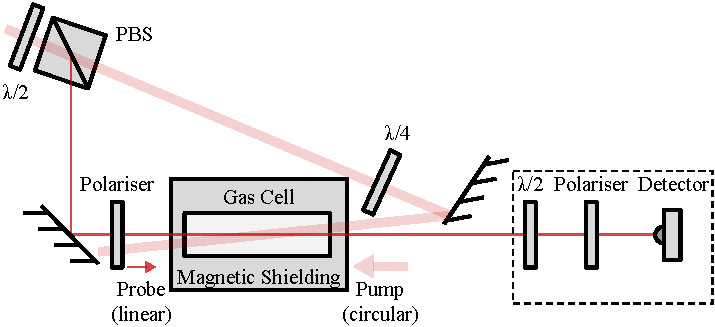
\includegraphics{part1/Figs/PolSpecWieman.pdf}
\caption{A schematic of the \gls{ps} setup initially suggested by Wieman and H\"ansch~\cite{wieman_doppler-free_1976}. The polariser by the detector is a linear polariser crossed with the linear polariser before the gas cell.}
\label{figure:wieman_doppler-free_schematic}
\end{figure}

Pearson et al. proposed the alternative method of using a balanced polarimeter, shown in Figure~\ref{figure:pol_spec_schematic}, which provides a background-free signal with peak-to-peak height more than an order of magnitude greater than with the crossed polariser method~\cite{pearman_polarization_2002,yoshikawa_frequency_2003}.

\subsubsection{Co-propagating Beams}

Wieman and H\"anch's initial proposal for \gls{ps} used a mirror next to the probe beamline to angle the pump beam such that it was \emph{almost} counter-propagating with the probe beam, as shown in Figure~\ref{figure:wieman_doppler-free_schematic}.
In saturated absorption spectroscopy imperfect alignment of the pump and probe results in geometric broadening of the spectral features and a reduction in the overlap region and thus the number of atoms involved and the degree of signal produced~\cite{himsworth_rubidium_2010}.
\Gls{ps} does not rely on the doppler-shifted velocities of the atoms involved and thus does not suffer from geometric broadening but the signal strength can be improved with fully counter-propagated beams.

Many saturated absorption spectroscopy setups use arrangements similar to the \gls{ps} setup shown in Figure~\ref{figure:wieman_doppler-free_schematic} in order to get the pump and probe beam to approximately counter-propagate however the layout shown in Figure~\ref{figure:satabs} provides a much simpler arrangement with anti-parallel beams and fewer required optics.
Similarly the \gls{ps} layout has been improved with the use of a non-polarising beam splitter to reflect the pump beam into the gas cell without interferring with the pump's circular polarisation or the probes rotated linear polarisation.
This gives the pump and probe beams the maximum interaction volume and maximises the signal produced.

\subsection{Fast Theory}

\subsection{Developments}

\subsubsection{High bandwidth feedback}


\subsection{Experimental Setup (with details - fibres, calcite, etc.)}

